%============================ MAIN DOCUMENT ================================
% define document class
\documentclass[
	a4paper               % paper format
	open=any, % Chapters start on even and uneven pages, remove for print
%	,10.5pt               % fontsize
%	,BCOR=18mm            % Binding correction
	,bibliography=totoc   % If enabled add bibliography to TOC
	,listof=totoc         % If enabled add lists to TOC
%	,bilingual
	,monolingual
]{bfhthesis}              % KOMA-script report

% TExt styling
\usepackage[
	hidelinks,
	pdfusetitle,
]{hyperref}
\usepackage{parskip}

% to have a smaller document, compression of : fonts, page stream, sobject streams
\pdfcompresslevel=9
\pdfobjcompresslevel=3


% to fix numbering of pages beeing cut at the bottom
\usepackage[a4paper,includefoot,bottom=25mm,left=15mm,right=15mm,top=15mm]{geometry}
\setlength{\footskip}{15mm}


%table styles
\usepackage{ltablex} % Combines longtable + tabularx
\usepackage[table]{xcolor}
\usepackage{tabularx,array,booktabs,multirow,graphicx,makecell}
%\usepackage[margin=15mm]{geometry}
\usepackage{ragged2e}
\usepackage{longtable,booktabs,array}
\usepackage{pdflscape}

% Define column type for wrapped text
\newcolumntype{L}{>{\RaggedRight\arraybackslash}X}
% Komfort: zentrierte p-Spalte
\newcolumntype{C}[1]{>{\centering\arraybackslash}p{#1}}
\newcolumntype{L}[1]{>{\raggedright\arraybackslash}p{#1}}
\newcolumntype{C}[1]{>{\centering\arraybackslash}p{#1}}

% for images which can be placed where they fit
\usepackage{graphicx}
\usepackage{float}

% for style of sql text to show correct code highlighting
\usepackage{listings}
\usepackage{xcolor}
\lstdefinestyle{sqlstyle}{
  language=SQL,
  basicstyle=\ttfamily\small,
  keywordstyle=\color{blue},
  commentstyle=\color{gray},
  stringstyle=\color{red},
  showstringspaces=false,
  frame=single
}
\lstdefinelanguage{json}{
    basicstyle=\ttfamily\small,
    numbers=none,
    showstringspaces=false,
    breaklines=true,
    frame=single,
    morestring=[b]",
    stringstyle=\color{blue},
    literate=
     *{0}{{{\color{magenta}0}}}{1}
      {1}{{{\color{magenta}1}}}{1}
      {2}{{{\color{magenta}2}}}{1}
      {3}{{{\color{magenta}3}}}{1}
      {4}{{{\color{magenta}4}}}{1}
      {5}{{{\color{magenta}5}}}{1}
      {6}{{{\color{magenta}6}}}{1}
      {7}{{{\color{magenta}7}}}{1}
      {8}{{{\color{magenta}8}}}{1}
      {9}{{{\color{magenta}9}}}{1}
      {:}{{{\color{black}{:}}}}{1}
      {,}{{{\color{black}{,}}}}{1}
      {\{}{{{\color{black}{\{}}}}{1}
      {\}}{{{\color{black}{\}}}}}{1}
      {[}{{{\color{black}{[}}}}{1}
      {]}{{{\color{black}{]}}}}{1}
}

% for cite different apearance
\hypersetup{hidelinks=false, colorlinks=true}
\hypersetup{
  citecolor=blue!60!black,
  linkcolor=black,
  urlcolor=blue!60!black
}


% for 2 column itemized lists
\usepackage{multicol}


% for Pseudo codes
\usepackage{algorithm}
\usepackage{algpseudocode}


\keepXColumns % ensures column widths stay consistent over pages

% --- Farben (an die Grafik angelehnt) ---
\definecolor{riskgreen}{HTML}{9AC88F}   % grün (low)
\definecolor{riskyellow}{HTML}{FFF2A8}  % gelb
\definecolor{riskorange}{HTML}{F4C37D}  % orange
\definecolor{riskred}{HTML}{E06666}     % rot
\definecolor{riskgrey}{HTML}{D9D9D9}    % Kopf-/Randgrau


% glossaries and bibliography
\usepackage{glossaries}
\usepackage[backend=biber,style=authoryear]{biblatex}
\addbibresource{MTE7102_DataQualityVisuals.bib} %  JabRef-as bibliography GUI
\makeglossaries

\newglossaryentry{PoC}{
    name={Proof of concept (POC)},  
    text={PoC},
description={Proof of concept (POC), also known as proof of principle, is a realization of a certain method or idea in order to demonstrate its feasibility, or a demonstration in principle with the aim of verifying that some concept or theory has practical potential. A proof of concept is usually small and may or may not be complete}}

\newglossaryentry{DQ}{
    name={Data Quality (DQ)},  
    text={data quality},
description={Data quality refers to the state of qualitative or quantitative pieces of information. There are many definitions of data quality, but data is generally considered high quality if it is "fit for [its] intended uses in operations, decision making and planning". Data is deemed of high quality if it correctly represents the real-world construct to which it refers. Apart from these definitions, as the number of data sources increases, the question of internal data consistency becomes significant, regardless of fitness for use for any particular external purpose.}}

\newglossaryentry{DA}{
    name={Data Availability (DA)},  
    text={data availability},
description={Data availability, in the context of this document, refers to whether the data is accessible e.g. whether a report can be retrieved and used when needed.}}


\newglossaryentry{BizDevOps}{
    name={BizDevOps},  
    text={BizDevOps},
description={ BizDevOps extends DevOps by including the business side.
In this constellation, the business becomes part of the team.
This setup improves communication between developers and the people requesting the work.}}

\newglossaryentry{ASTV}{
    name={ASTV},  
    text={ASTV},
description={An abbreviation used at Swiss Post within the postal services.
It is an acronym for the German terms: “Aufgabe” –> Receiving, “Sortierung” –> Sorting, “Transport” –> Transport, “Verzollung” –> Customs clearance. This abbreviation encompasses the entire postal process, except for the delivery step.}}

\newglossaryentry{ASTVZ}{
    name={ASTVZ},  
    text={ASTVZ},
    description={An abbreviation used at Swiss Post within the postal services.
    It is an acronym for the German terms: “Aufgabe” → Receiving, “Sortierung” → Sorting, “Transport” → Transport, “Verzollung” → Customs clearance, and “Zustellung” → Delivery. This abbreviation encompasses the entire postal process, from receiving a mail piece until it is delivered.}
}

\newglossaryentry{DandF}{
    name={D \& F, Delivery and Finance},  
    text={D \& F},
    description={The Delivery and Finance team is a BizDevOps team in DWH LS OPS handling requirements related to delivery and finance, including regional controlling and process controlling.}
}

\newglossaryentry{MPP}{
    name={MPP Mengenplanung und Prognose Pakete},  
    text={MPP},
    description={MPP Parcel Volume Planning and Forecasting is a team within Swiss Post. It is responsible for improving current planning and forecasting methods. Based on this information, important decisions are made, such as determining the personnel required for peak periods like the Christmas season with increased parcel volumes. The team analyses current data sources and aims to provide more precise methods and data sources for the process.}
}


\newglossaryentry{DWHLSOPS}{
    name={DWH LS OPS},  
    text={DWH LS OPS},
description={A Swiss post abreviation, DWH -> "Data Warehouse", LS -> "Logistic Services", OPS -> "Operations". Together, this refers to the Data Warehouse that supports and manages the operational processes of the postal logistics services.}}

\newglossaryentry{SmartGoals}{
    name={Smart Goals},  
    text={SmartGoals},
description={S.M.A.R.T. (or SMART) is an acronym used as a mnemonic device to establish criteria for effective goal-setting and objective development. The S.M.A.R.T. criteria he proposes are as follows: Specific: Targeting a particular area for improvement, Measurable: Quantifying, or at least suggesting, an indicator of progress, Assignable: Defining responsibility clearly, Realistic: Outlining attainable results with available resources, Time-related: Including a timeline for expected results}}

\newglossaryentry{riskappetite}{
    name={Risk Appetite},  
    text={risk appetite},
description={Risk appetite is a term used in risk management.
It describes an individual’s perception and tolerance of risk.
Even when two people are facing the same risk, they may perceive its severity and probability differently, based on their personal risk appetite.}}

\newglossaryentry{NRT}{
    name={Near Realtme},  
    text={near realtime},
description={Near Real Time (NRT) refers to data that becomes available for reporting almost immediately after the event occurs, but not instantly.
The time window in which data is considered near real time can vary depending on the use case and the type of data.
For example, NRT might mean that data is available within 5 minutes up to 1 hour after the event has happened.}}

\newglossaryentry{RealTime}{
    name={Real Time},  
    text={real time},
description={Real-time data (RTD) is information that is delivered immediately after collection. There is no delay in the timeliness of the information provided. Real-time data is often used for navigation or tracking.}}

\newglossaryentry{KafkaTopics}{
    name={Kafka Topics},  
    text={Kafka topics},
description={A Kafka topic is a core component of Apache Kafka.
It is a named storage structure where producers write messages or data streams.
The content of the topic can then be read and processed by consumers.}}

\newglossaryentry{ETL}{
    name={ETL},  
    text={ETL},
description={Extract, transform, load (ETL) is a three-phase computing process where data is extracted from an input source, transformed (including cleaning), and loaded into an output data container.}}

\newglossaryentry{analyticalreporting}{
    name={Analytical Reporting},  
    text={analytical reporting},
description={Analytical Reporting is focusing on interpreting data. To be able to make management decisions over multiple days, weeks or months. It is fundamentally different to operational reporting which monitors the current status e.g. to check if machines are operating without errors.}}

\newglossaryentry{sortingcenter}{
    name={Sorting Center},  
    text={sorting center },
description={In the postal services of Swiss Post, sorting centers are an essential part of the logistics process for handling letters and parcels. Items are first collected and sent to regional centralized facilities, where they are either: routed to sorting centers in other regions, or processed locally and dispatched to the distribution network of the current region. These centers enable efficient processing and routing of mail within Switzerland and across regions.}}

\newglossaryentry{onetoonemigrations}{
    name={One to One Migrations},  
    text={one-to-one migrations},
description={In the context of reporting, a one-to-one migration refers to rebuilding an existing report exactly as it is, but on a different software or hardware platform.
The structure, logic, and content of the report remain unchanged only the underlying technology is replaced.}}

\newglossaryentry{greenfield}{
    name={Greenfield},  
    text={greenfield},
description={A greenfield refers to a system landscape where no prior system exists.
In IT, a greenfield project means that a new system is built from scratch, without having to consider or integrate with any existing legacy systems. Because there is no predecessor system, development can proceed more freely, without compatibility constraints — which often makes the implementation simpler and more flexible compared to a migration or redesign of an existing system (a brownfield).}}

\newglossaryentry{MVP}{
    name={MVP},  
    text={MVP},
description={A Minimal Viable Product (MVP) is the simplest version of a system that successfully fulfils a specific use case.
It is developed with just the core functionality needed to provide value to users. An MVP can serve two main purposes: to demonstrate that a concept or method is feasible (proof of concept), or as an initial implementation that will later be improved through further development and updates.}}

\newglossaryentry{highlevel}{
    name={High Level},  
    text={high level},
description={High level refers to viewing a use case from a general or abstract perspective, rather than analyzing all details.
It focuses on the overall picture instead of individual elements. Instead of examining every single event during a day, a high-level analysis would simply check whether most events fall within the expected range during that day}}


\newglossaryentry{infoblock}{
    name={Infoblock},  
    text={infoblock},
    description={Infoblock (at Swiss Post in the context of AWS data storage)
An Infoblock is a standardized data product that is provided within the data architecture of Swiss Post for reporting and analysis purposes. It serves as a logical unit of processed and quality-assured data that is extracted from different source systems, transformed, and stored in a consistent structure in the AWS cloud. This concept is similar to data products as defined in modern data management practices.}
}

\newglossaryentry{NDA}{
    name={NDA},
    text={NDA},
    description={A non-disclosure agreement (NDA), also known as a confidentiality agreement (CA), confidential disclosure agreement (CDA), proprietary information agreement (PIA) or secrecy agreement (SA), is a legal contract or part of a contract between at least two parties that outlines confidential material, knowledge, or information that the parties wish to share with one another for certain purposes, but wish to restrict access to}}


\newglossaryentry{IP}{
    name={IP},
    text={IP},
    description={Intellectual property (IP) is a category of property that includes intangible creations of the human intellect}
}


\newglossaryentry{SAC}{
    name={SAC, SAP Analytics Cloud},
    text={SAC },
    description={SAC, SAP Analytics Cloud is a plattform for online analytical reporting. It allows to show data in tables and dashboards and allows Reporting and predictive analysis.}
}

\newglossaryentry{DSP}{
    name={DSP, SAP Datasphere},
    text={DSP},
    description={DSP (SAP Datasphere) enables the creation of data models that integrate SAP and non-SAP data sources. These sources can include databases as well as Excel files. The data sources can then be further joined and aggregated.}
}

\newglossaryentry{spark}{
    name={Apache Spark},
    text={Spark},
    description={Apache Spark is an open-source unified analytics engine for large-scale data processing. Spark provides an interface for programming clusters with implicit data parallelism and fault tolerance.}}

\newglossaryentry{aws}{
    name={Amazon Web Services, Inc. (AWS) },
    text={Amazon Web Services (AWS) },
    description={Amazon Web Services, Inc. (AWS) is a subsidiary of Amazon that provides on-demand cloud computing platforms and APIs to individuals, companies, and governments, on a metered, pay-as-you-go basis.}}

\newglossaryentry{athena}{
    name={Amazon Athena},
    text={Athena},
    description={Amazon Athena runs interactive queries directly against data in Amazon S3.}
}

\newglossaryentry{datalineageview}{
name={Data Lineage View},
 text={data lineage view},
description={A visual representation in SAP DSP that displays which data sources are used and how they are connected. It shows joins and aggregations and allows users to navigate through a hierarchical tree structure to understand data flow, transformations, and dependencies.}
}

\newglossaryentry{analyticmodel}{
name={Analytic Model},
 text={Analytic Model},
description={A structured model in SAP DSP used as the foundation for reporting and analytics. It can consist of multiple data sources, joins between those sources, label transformations, and aggregations that prepare the data for analytical consumption.}
}

\newglossaryentry{PO}{
    name={Product Owner (PO)},  
    text={product owner (PO)},
description={Each scrum team has one product owner. The product owner focuses on the business side of product development and spends the majority of time liaising with stakeholders and the team. The role is intended to primarily represent the product's stakeholders, the voice of the customer, or the desires of a committee, and bears responsibility for the delivery of business results.}}

\newglossaryentry{postday}{
    name={Post day},  
    text={post day},
    description={The post day starts at 06:00 AM and lasts until 05:59 AM the next day. This is the essential date format used by Swiss Post for reporting.}
}

\newglossaryentry{messageprocessing}{
    name={Message processing},  
    text={message processing},  
    description={Sendungsverarbeitung is a central infoblock containing data from sorting systems. It allows mail pieces to be followed through the sorting process and enables various reports to be generated.}
}

\newglossaryentry{curated}{
    name={Curated database layer},  
    text={curated},  
    description={The curated database layer is the first layer in the Swiss Post DWH setup in which data is cleaned and standardised and duplicates are removed. This occurs after the data is received in a raw format.}
}

\newglossaryentry{RX}{
    name={Rollbox (RX)},  
    text={RX},  
    description={The rollbox (RX) is used to temporarily transport parcels throughout the Swiss Post workflow. It can hold many mail pieces and is used to move them between different processing areas, making it an essential component of parcel handling at Swiss Post.}
}

\newglossaryentry{principal}{
    name={Principal},
    text={principal},
    description={The principal seniority level represents long-term experience in a professional role. A principal features extensive experience and domain knowledge and has a strategic influence across teams or systems. They will often define standards and lead in decision-making.}
}

\newglossaryentry{senioritylevel}{
    name={Seniority level},
    text={seniority level},
    description={The seniority level describes the experience and responsibilities a worker has amassed in their current role. Seniority levels are used to distinguish between juniors, seniors, principals, and higher levels of experience.}
}

\newglossaryentry{IAM}{
    name={Identity and Access Management (IAM)},
    text={IAM},
    description={Identity and Access Management (IAM) is a system used to assign roles and permissions to users within large organisations. It allows permissions for office access, software usage, and permission levels in third-party software to be set up. It also consists of GUI and interfaces that allow assigning and controlling user permissions.}
}


\newglossaryentry{DQM}{
    name={Data Quality Management (DQM)},  
    text={DQM},
    description={Data quality management is the management of data quality topics. It describes how data quality is handled in a company. However, in this document, most references to DQM refer to the IT team working at Swiss Post on the DQM topic. This team is implementing defined software that is intended to promote improvements in data quality.}
}

\newglossaryentry{AWSS3}{
    name={Amazon S3},
    text={Amazon S3},
    description={Amazon Simple Storage Service (S3) is a service offered by Amazon Web Services (AWS) that provides object storage through a web service interface. Amazon S3 uses the same scalable storage infrastructure that Amazon.com uses to run its e-commerce network.}
}

\newglossaryentry{CTE}{
    name={CTE},
    text={CTE},
    description={A common table expression, or CTE, (in SQL) is a temporary named result set, derived from a simple query and defined within the execution scope of a SELECT, INSERT, UPDATE, or DELETE statement. CTEs can be thought of as alternatives to derived tables (subquery), views, and inline user-defined functions.}
}

\newglossaryentry{DWH}{
    name={DWH},
    text={DWH},
    description={In computing, a data warehouse (DW or DWH), also known as an enterprise data warehouse (EDW), is a system used for reporting and data analysis and is a core component of business intelligence. Data warehouses are central repositories of data integrated from disparate sources.}
}
\newglossaryentry{businessanalyst}{
    name={Business analyst},
    text={business analyst},
    description={A business analyst (BA) is a person who processes, interprets and documents business processes, products, services and software through analysis of data. The role of a business analyst is to ensure business efficiency increases through their knowledge of both IT and business function.}
}

\newglossaryentry{logisticservice}{
    name={LS, logistic service},
    text={logistic service},
    description={A business analyst (BA) is a person who processes, interprets and documents business processes, products, services and software through analysis of data. The role of a business analyst is to ensure business efficiency increases through their knowledge of both IT and business function.}
}

\newglossaryentry{logisticservices}{
    name={LS, Logistics Services},
    text={logistics services},
    description={Logistics Services (LS) is responsible for efficient and secure logistics of letters, printed matter and newspapers, as well as parcels, goods and merchandise in Switzerland and internationally. Logistics Services is the largest business unit of Swiss Post and makes a substantial contribution to the company’s success with over 21 000 employees.}
}

\newglossaryentry{AWSGlue}{
    name={AWS Glue},
    text={AWS Glue},
    description={AWS Glue is a serverless data integration service that makes it easy for analytics users to discover, prepare, move, and integrate data from multiple sources. You can use it for analytics, machine learning, and application development. It also includes additional productivity and data ops tooling for authoring, running jobs, and implementing business workflows. https://docs.aws.amazon.com/glue/latest/dg/what-is-glue.html}
}

\newglossaryentry{KPI}{
    name={KPI, key performance indicator},
    text={KPI},
    description={A performance indicator or key performance indicator (KPI) is a type of performance measurement. KPIs evaluate the success of an organization or of a particular activity (such as projects, programs, products and other initiatives) in which it engages. KPIs provide a focus for strategic and operational improvement, create an analytical basis for decision making and help focus attention on what matters most.}
}

\newglossaryentry{scrum}{
    name={Scrum},
    text={Scrum},
    description={Scrum is an agile team collaboration framework commonly used in software development and other industries. Scrum prescribes for teams to break work into goals to be completed within time-boxed iterations, called sprints.}
}

\newglossaryentry{kanban}{
    name={Kanban},
    text={Kanban},
    description={Kanban (Japanese: meaning signboard) is a scheduling system for lean manufacturing (also called just-in-time manufacturing). Taiichi Ohno, an industrial engineer at Toyota, developed kanban to improve manufacturing efficiency. The system takes its name from the cards that track production within a factory.}
}

\newglossaryentry{JourFixe}{
    name={Jour Fixe},
    text={Jour Fixe},
    description={A Jour Fixe is a weekly meeting used in project management to provide updates on progress, issues encountered during work, and problems that remain unresolved and require assistance. It serves to maintain communication and alignment with stakeholders.}
}

\newglossaryentry{epic}{
    name={Epic},
    text={epic},
    description={Epics are large bodies of work in Agile that are broken down into smaller user stories for incremental delivery. They help teams organize, prioritize, and track progress toward bigger goals while maintaining agility.}
}

\newglossaryentry{MIAR}{
    name={MIAR},
    text={MIAR},
    description={MIAR is the internal reporting and project effort tracking system used at Swiss Post. It is integrated with applications for working time recording, such as check-in and check-out. It allows employees to allocate worked hours to projects, which in turn enables monitoring of project efforts.}
}

\newglossaryentry{WYSIWYG}{
    name={WYSIWYG (what you see is what you get)},
    text={WYSIWYG},
    description={In computing, WYSIWYG  (what you see is what you get) is software that allows content to be edited in a form that resembles its appearance when printed or displayed as a finished product, such as a printed document, web page, or slide presentation. WYSIWYG implies a user interface that allows the user to view something very similar to the result while the document is being created.}
}

\newglossaryentry{PBI}{
    name={Microsoft Power BI (PBI) },
    text={Power BI},
    description={Microsoft Power BI (PBI) is an interactive data visualization software product developed by Microsoft with a primary focus on business intelligence (BI). It is part of the Microsoft Power Platform. Power BI is a collection of software services, apps, and connectors that work together to turn various sources of data into static and interactive data visualizations.}
}

\newglossaryentry{PC}{
    name={Parcel center},
    text={PC},
    description={A parcel center is a large sorting center for parcels at Swiss Post. Each region has one parcel center, which serves as the main hub for parcel sorting. Every parcel is first gathered at a parcel center and later distributed to smaller regional parcel centers if its delivery is not scheduled for the immediate vicinity of the center.}
}

\newglossaryentry{RPC}{
    name={Regional parcel center},
    text={RPC},
    description={A regional parcel center is a smaller sorting center for parcels at Swiss Post. Multiple regional parcel centers are located within one region and handle parcels for smaller geographic areas.}
}

\newglossaryentry{region}{
    name={Region},
    text={region},
    description={Swiss Post organises its postal services into four regions covering the whole of Switzerland. These regions are West, Middle, East, and South. The regions are not based on cantonal borders and may split cantons between regions.}
}

\newglossaryentry{BI}{
    name={Business intelligence},
    text={BI},
    description={Business intelligence (BI) consists of strategies, methodologies, and technologies used by enterprises for data analysis and management of business information to inform business strategies and business operations. Common functions of BI technologies include reporting, online analytical processing, analytics, dashboard development, data mining, process mining, complex event processing, business performance management, benchmarking, text mining, predictive analytics, and prescriptive analytics.}
}

\newglossaryentry{AWSGlueDQ}{
    name={AWS Glue Data Quality},
    text={AWS Glue Data Quality},
    description={AWS Glue Data Quality allows you to measure and monitor the quality of your data so that you can make good business decisions. Built on top of the open-source DeeQu framework, AWS Glue Data Quality provides a managed, serverless experience. AWS Glue Data Quality works with Data Quality Definition Language (DQDL), which is a domain specific language that you use to define data quality rules.}
}

\newglossaryentry{PyDeequ}{
    name={PyDeequ},
    text={PyDeequ},
    description={PyDeequ is a Python API for Deequ, a library built on top of Apache Spark for defining "unit tests for data", which measure data quality in large datasets. PyDeequ is written to support usage of Deequ in Python.}
}

\newglossaryentry{starShema}{
    name={Star Schema},
    text={star schema},
    description={A dimensional data modelling approach following the Kimball methodology, consisting of a central fact table linked to multiple denormalised dimension tables. The denormalisation is performed to improve the performance of analytical queries. It is widely used in data warehouses and business intelligence systems.}
}


\begin{document}

\frontmatter

\title{Specialisation Project 2 MTE7102}
\subtitle{Enhancing User Confidence in Report Timeliness and Data Accuracy through Data Quality and Availability Checks}
\author{Roland Angelo Roccaro}
\institution{Bern University of Applied Sciences}
\department{School of Engineering and Computer Science}
\institute{Master of Science in Engineering}
\version{1.0}
\titlegraphic{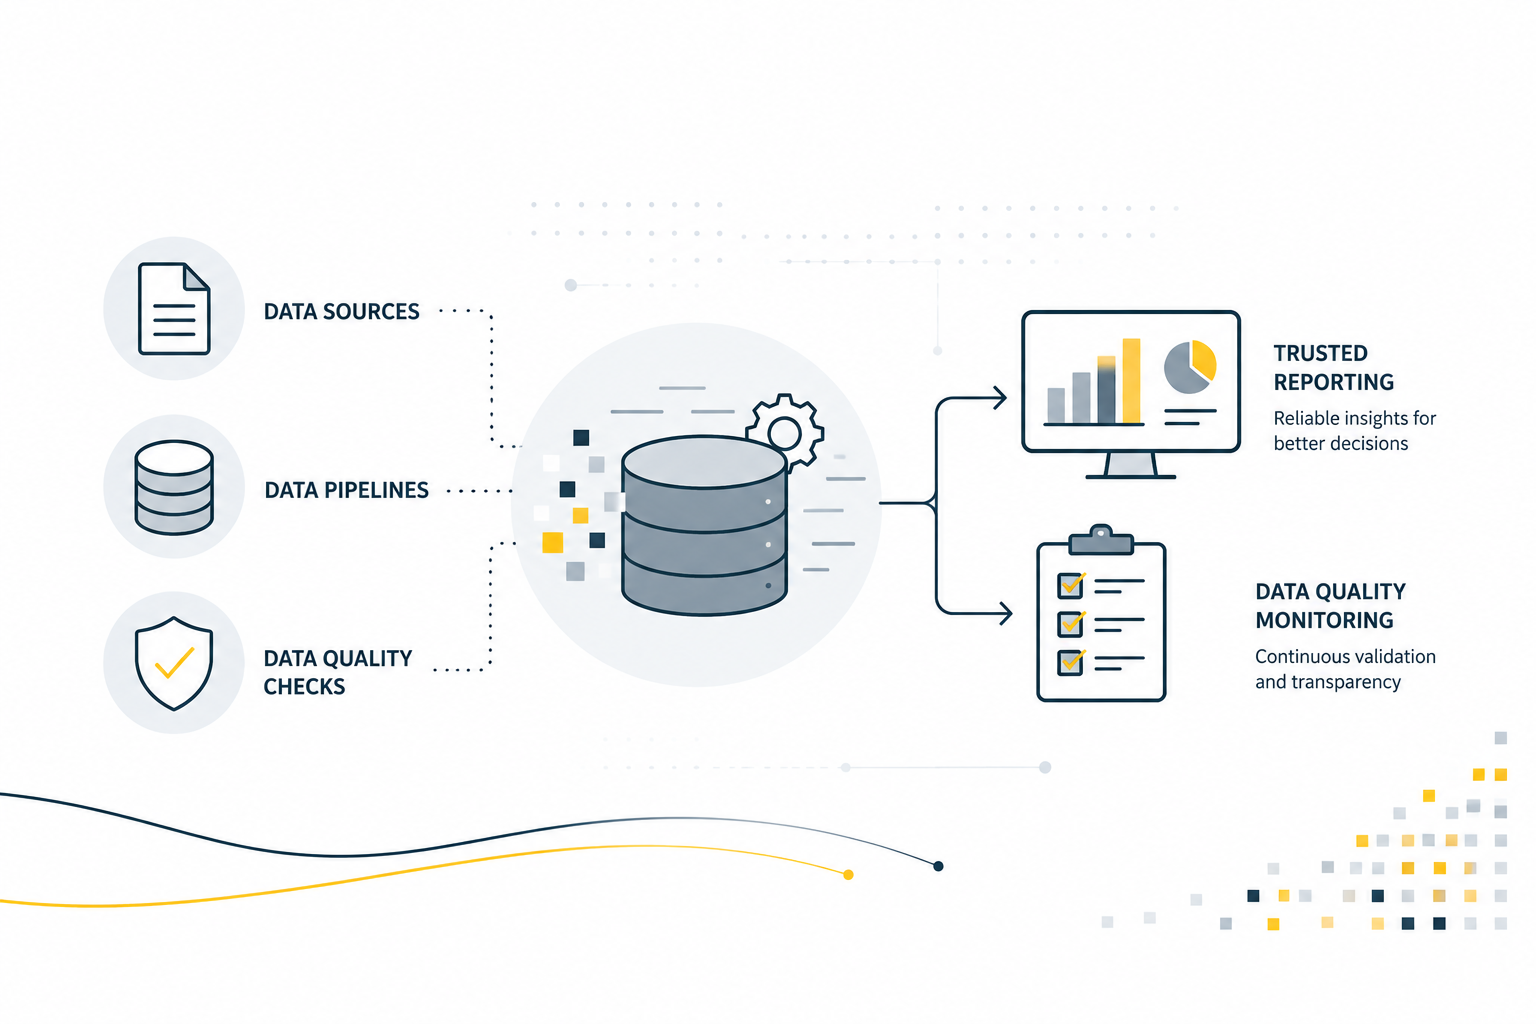
\includegraphics[width=\width]{./content/img/TitlePage_V1.png}}
\advisor{Prof. Dr. Kenneth A. Ritley}
%\coadvisor{Todo Mr. or Mrs. Undefined}
\projectpartner{Swiss Post}
%\expert{Todo Mr. or Mrs. Undefined}
\degreeprogram{Master of Science MSc in Engineering: Profile Data Science}

%----------------  BFH tile page   -----------------------------------------
\maketitle

% chapter and abstract imports as input


\addchap{Abstract}

This project addresses the next mandatory steps bridging from a first project on the topic towards the master's thesis. The problem addressed is the identification of a suitable tool with which the automation of the current data quality checks can be performed. During the course of this work, another main goal is to provide the business with tools that can assist them with the usage of new data sources. The Power BI report for the daily checks of the message processing data did exactly that, employing improved visualisations developed by the project team. All this was done while applying the DevOps principles at Swiss Post and implementing user feedback received while building the report for stakeholders.

As a next step, the search for a DQM tool was addressed by following the team during the setup of requirement lists and the evaluation of tools, including demonstrations of such tools. However, as the decision on the tool had not yet been taken by the end of this project, the way forward was defined together with the DWH LS OPS solution architect in a meeting. The monitoring that was set up to check the uptime of jobs such as ETL jobs was selected for testing in its second application, namely running checks on data. This tool was able to run counts on queries executed through Amazon Athena. However, the function had not yet been properly tested. Therefore, the project team carried out tests to verify whether this tool could be applied to the use case defined for the master's thesis. This use case was the automation of the data quality checks performed daily, which were part of the previous research.

With this information, the next step was to test this possible data quality tool, which was developed during the AWS Modernisation and was part of the full BizDevOps team until the end of May. Until then, knowledge transfer sessions were performed. After these transfers, a test was derived based on the full use case of the master's thesis, reducing its complexity and amount of data to perform only one count of one specific sorting centre for one event rather than for every sorting centre.

Finally, it was possible to evaluate the given solution as suitable for the master's thesis. This included not only the setup of a test case but also the setup of the required infrastructure. Thus, everything required for the master's thesis has been tested successfully. The details of this research, the additions to the solution landscape, and the implementation are part of the documentation that follows.


%------------ TABLEOFCONTENTS ----------------
\tableofcontents

% optional:
% \printglossary[type=\acronymtype,title={List of Acronyms}]



%------------ START MAIN PART ----------------

\mainmatter

\chapter{Introduction}

Since mankind first began making plans, they were based on the available description of the environment. This approach continued into modern times, although the nature of the predictions has changed. People no longer plan which animal to hunt or when to produce stone tools, but instead how many people the postal service should hire for the Christmas season. These decisions require data, and in order to make the right decisions, the data must be available in the right time, in the right context, for the right people and naturally be correct. This makes data one of the most important assets in a company \cite{economist2017_dataoil}. Data allow companies to gain an edge over competitors, analyse clients’ wishes, or improve internal processes. This is where the relevance of this project emerges. 

Swiss Post requires \gls{DA} and \gls{DQ} in its reporting for decision making. This project analyses the current state of a specific data area of Swiss Post and provides steps toward improvements.
This chapter familiarises the reader with the topic. It presents the background of the project at Swiss Post and delves into the motivation behind it. It then further explains the business relevance, demonstrating why it is both important and beneficial for Swiss Post to invest in the topic. Next, the problem statement is addressed, explaining what this project aims to solve. After the problem statement, the scope and limitations of the project are outlined more clearly. Finally, a brief overview of the expected outcomes of the project is provided. This chapter concludes with a preview of the document’s structure.


\section{Background}
\label{IntroBackground}
Swiss Post is Switzerland’s national service provider, active not only in mail and parcel logistics but also in passenger transport (PostAuto), financial services (PostFinance), and various digital and e-government solutions. Its workforce of approximately 45’000 employees and nationwide infrastructure move millions of items and people every day, supported by highly automated sorting centres and extensive data flows \cite{postGeschäftsbericht2024}. In such a diversified organisation, \gls{analyticalreporting} is essential for strategic steering, operational planning, and maintaining service quality across business units. The organisational structure of Swiss Post is shown in the following diagram.

\begin{figure}[H]
    \centering
    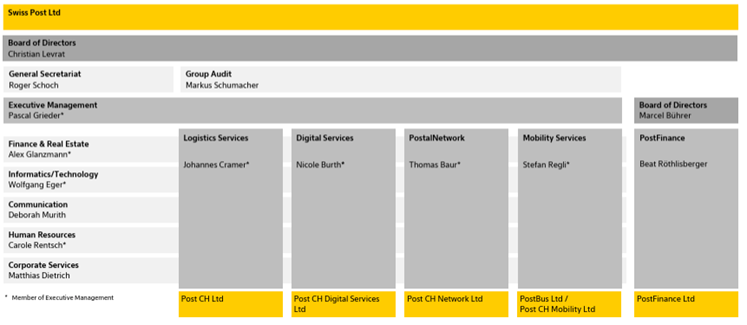
\includegraphics[width=0.8\textwidth]{./content/img/Post_external/OrgStruktur_Online.png}
    \caption{Organisational structure of Swiss Post (online version)}
    \label{fig:orgstruktur_online}
\end{figure}


\subsection*{The full mail piece lifecycle}
Within this large organisation, the project takes place within a specialised team supporting the entire lifecycle of logistics for mail and parcel delivery. In German, this lifecycle covers every step from A to Z, \gls{ASTVZ}, which stands for:
\begin{itemize}
    \item \textbf{A}nnahme: Receiving, where parcels and mail are accepted and registered by Swiss Post to be sent through its network
    \item \textbf{S}ortierung: Sorting, the process during which received mail pieces are separated by destination and routed to the next process step, either further sorting or delivery
    \item \textbf{T}ransport: Transport includes the movement between sorting plants and delivery sectors
    \item \textbf{V}erzollung: Customs clearance handles international parcels and letters, including the required customs checks and documentation
    \item \textbf{Z}ustellung: Delivery is the final process step for every item; it is delivered by the staff of Swiss Post
\end{itemize}

However, this process is more easily visualised using the future vision of Swiss Post. In particular, the version tailored for the IT domain is well suited to describing the project environment. Starting from the top left with the A or V step, followed by S, T, and Z, the process progresses towards the bottom right.

\begin{figure}[H]
    \centering
    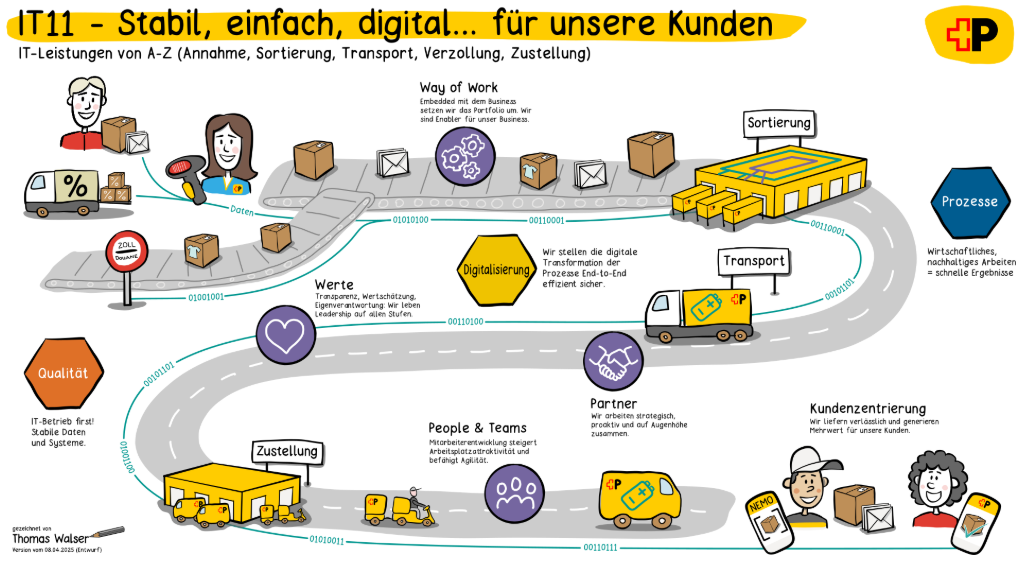
\includegraphics[width=0.8\textwidth]{./content/img/Post_internal/06-12-2025_20-16-16.png}
    \caption{Future way of work illustrating the full postal delivery workflow from receiving an item to delivery.}
    \label{fig:future_way_of_work}
\end{figure}


\subsection*{DWH LS OPS}
\label{IntroDWHLSOPSTasks}

The project team supports the \textbf{D}ata \textbf{W}are\textbf{h}ouse of \textbf{L}ogistic \textbf{S}ervices \textbf{Op}eration\textbf{s} (\gls{DWHLSOPS}). This \textbf{Busi}ness \textbf{Dev}elopment \textbf{Op}eration\textbf{s} (\gls{BizDevOps}) team is located within the organisational structure of the Logistics Services vertical and the Informatics/Technology horizontal. It represents the single source of truth for \gls{analyticalreporting} at Swiss Post. In contrast to operational reporting, which focuses on real-time guidance for operational processes, analytical reporting focuses on aggregated insights for evaluation and planning. Examples of analytical reporting include working time, process time, and aggregations of sorted items. The stakeholders of the team distribute these reports to various task groups within postal services, such as sorting and delivery.

There are two reasons why a deeper understanding of analytical reporting is currently very important. First, the infrastructure for analytical reporting is transitioning from on-premise systems to the cloud. Second, in addition to the migration of reporting, the infrastructure at all Swiss Post \gls{sortingcenter} locations for parcels is undergoing fundamental changes. These changes may include complete modifications of data pipelines, which can make comparisons with previous figures impossible. Therefore, at this critical point in time, it is of utmost importance to maintain users’ trust in the data during this change process. The following figure illustrates the shift from the on-premise setup on the right-hand side to the target architecture using cloud hardware on the left-hand side.

\begin{figure}[H]
    \centering
    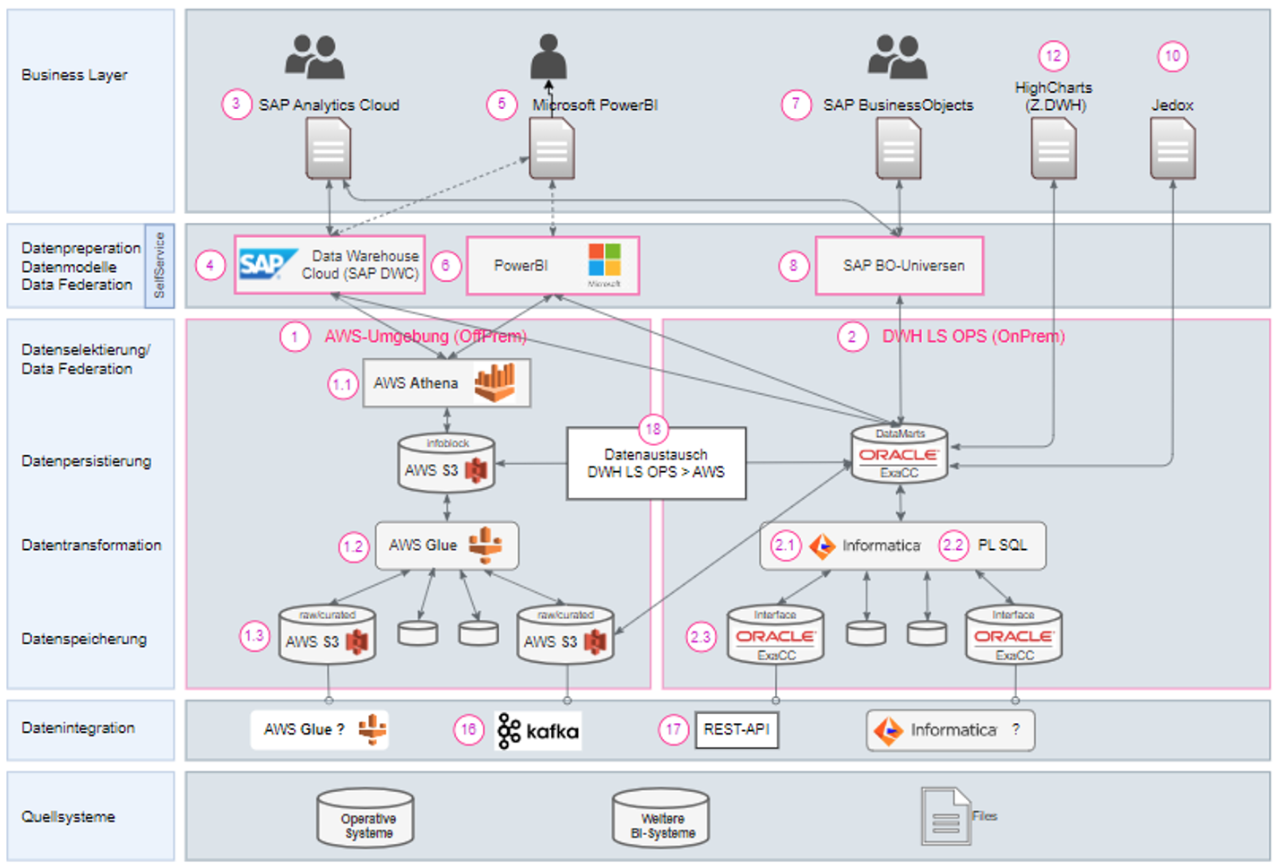
\includegraphics[width=0.8\textwidth]{./content/img/OnPrem_Cloud_Migration.png}
    \caption{The transition from an on-premise setup to a cloud-based target architecture.}
    \label{fig:on_prem_cloud_migration}
\end{figure}


\subsection*{Swiss Post sorting centers are cyber machines}
Swiss Post has built and operate a number of massive sorting centers located across Switzerland. These are far more than just mechanical warehouses or factories. Rather, these sorting centers are massive “cyber facilities” that include high-tech hardware but also high-tech IT systems to keep them running.

While the team handles use cases across the entire postal delivery workflow, this project initially focuses on supporting sorting data flows. Sorting at Swiss Post is the process of consolidating received items in centralised plants, to which letters and parcels are sent from regions across Switzerland. One such plant is located in Härkingen:

\begin{figure}[H]
    \centering
    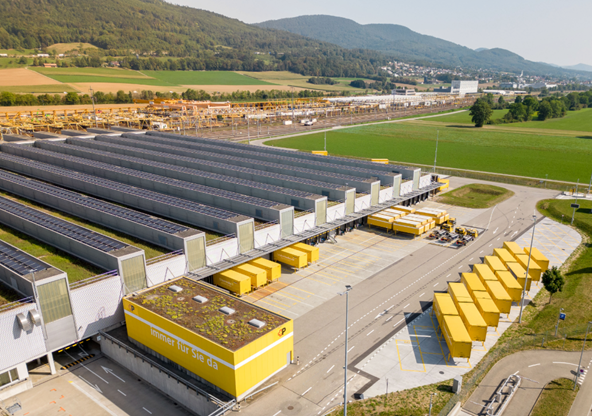
\includegraphics[width=0.8\textwidth]{./content/img/Post_external/Sortierzentrum_Aussen_Vogel.png}
    \caption{Aerial view of the Swiss Post sorting center in Härkingen.}
    \label{fig:sortierzentrum_haerkingen_aerial}
\end{figure}

Mail pieces are handled by workers and placed onto the automated sorting hardware of Swiss Post. This hardware enables the handling of up to 10’000 parcels per hour \cite{SwissPostHarkingenSort}. The system scans the received items and transports them through the plant via conveyor belts to their correct destinations, where they are discharged through chutes. These chutes are shown in the second image, including staff placing the parcels into roll boxes for further processing.

\begin{figure}[H]
    \centering
    \includegraphics[width=0.8\textwidth]{./content/img/Post_ExperienceHub/_DSC4975.jpg}
    \caption{Interior view of the automated sorting system in a Swiss Post sorting center.}
    \label{fig:sortierzentrum_innen_anlage}
\end{figure}
\begin{figure}[H]
    \centering
    \includegraphics[width=0.8\textwidth]{./content/img/Post_ExperienceHub/_DSC4916.jpg}
    \caption{Discharge chutes inside a Swiss Post sorting center, where parcels are released to their designated zones. Then put into rollboxes to get them to next processing steps.}
    \label{fig:sortierzentrum_innen_rutschen}
\end{figure}



\section{Motivation}
\label{IntroMotivation}
\textbf{Data quality} and \textbf{data availability} are central to the successful operations of any company. Even a company working in low-tech or non-IT industries \cite{basedconlDA} has basic but essential data needs, for example, information on who is working where and the addresses of clients and staff. Not having this data in the right quality or available to the right people at the right time will cause problems whenever the data needs to be used.

In the context of ongoing changes to the Swiss Post reporting infrastructure, keeping track of \gls{DA} and \gls{DQ} is challenging. These infrastructure-related changes comprise the construction of new reports, \gls{onetoonemigrations}, and the re-engineering of existing reports.
Since the topic of data quality in the Swiss Post operations area could be built from scratch, as if starting on a \gls{greenfield}, it became an ideal subject for a master’s thesis. 

Furthermore, the topic was not of the highest priority for Swiss Post, but it was still considered a valuable idea to pursue. The medium-priority nature of this project also allowed the topic to be divided into multiple steps, such as working from a PoC to an \gls{MVP} setup. Additionally, the medium priority regarding feature development in this area allowed for well-grounded research on the topic. All these aspects combined made it a suitable project leading to a master’s thesis.
Furthermore, due to the lack of automated data accuracy and data quality checks in the DWH LS OPS environment at the time of defining this project, this topic is highly relevant to the team responsible for both the operational and analytical reports that help guide the company. If the data is incorrect, wrong decisions are made; and if the data is unavailable, management cannot properly lead the staff. Thus, the topic is of high importance and business critical: data quality and availability help Swiss Post continue to deliver reliable services on a daily basis and enable IT to provide better assistance to staff throughout the postal process.

\begin{figure}[H]
    \centering
    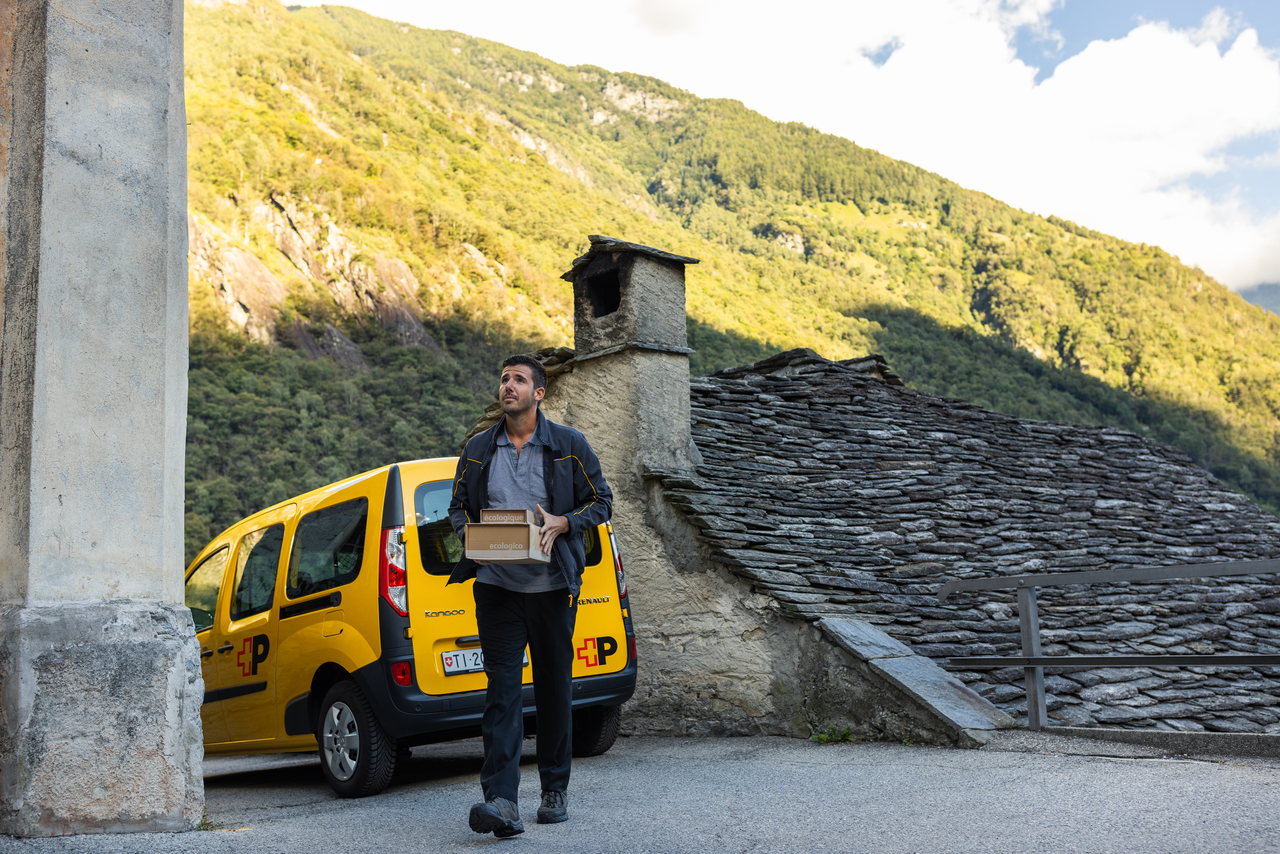
\includegraphics[width=0.8\textwidth]{./content/img/Post_ExperienceHub/Markenshooting_2021_Tessin_LS_059.png}
    \caption{Main customer touch point, delivery of a parcel}
    \label{fig:intro_parcel_mailman}
\end{figure}

\section{Problem statement}
The two key problems addressed in this project are, first, that data quality in this area of Swiss Post has so far been handled in an ad hoc manner, without formal definitions, frameworks, or an agreed set of KPIs; and second, that data quality is handled manually by the business at a \gls{highlevel} rather than being automated by the IT department. Both of these problems lead to issues not being detected early and to longer reaction times. As a further consequence, delays in data processing are not identified and targeted for systematic resolution, which in turn reduces management confidence in the reports. All of this prevents continuous improvement, as the current checks are neither documented nor stored in a way that allows follow-up analysis or structured refinement.


\section{Scope and boundaries}
This research focuses on the data availability and data quality challenges of the \gls{DWHLSOPS} \gls{BizDevOps} \gls{ASTV} teams at Swiss Post described in section \ref{IntroBackground}. To simplify the scope of this work, the first step of data retrieval, such as how data is stored from \gls{KafkaTopics}, is excluded. The scope begins with the curated and reporting layers in the \gls{ETL} process of the retrieved data. The aim of this project is to specifically provide solutions for the mentioned teams and not to offer a general solution or framework for the entire Swiss Post.


\section{Expected outcome}
The high-level goal of this master’s thesis pre-project is to demonstrate that automated data quality checks provide additional safety and can be calibrated to the needs of the business. Automated data quality checks refer to checks executed daily or upon data load, which are always carried out by systems without the need for manual interaction. More specifically, the project focuses on establishing the foundations for this goal by analysing the current situation and developing a proof of concept (\gls{PoC}). It will carefully document and explain the steps taken toward the proof of concept and, in this way, make the decisions made understandable. The success criterion of this project is to provide a PoC, or steps toward a PoC, that help reduce the costs of manual checks.




\section{Structure of the document}


This document is intended to guide the reader through the project in meaningful steps, explaining how the project is set up and executed, and then leading into the research and conclusions. It is structured in the following way. First, the document begins with the project management chapter, which explains the methods used during the project. It provides reasoning for tool choices where applicable and lists the tools and teams with which collaboration took place.
Next, the research chapter describes the problem in more detail. It clearly defines the specific and measurable goals of the project and presents the research sources used. This allows the reader to understand the decisions made and establishes the basis for the solution design. 
The subsequent solution design chapter explains how the problem statement is addressed. It describes the tools selected and how they interact with one another. This is followed by the implementation chapter, which presents the implementation of this design. It contains the work carried out by the project team and outlines any issues encountered. After the implementation, the target analysis chapter compares the expected outcome with the achieved outcome, assessing how many goals were reached and listing their fulfilment status. 
The document concludes with the critical review and lessons learned, summarising what went well and what did not, and offering specific suggestions on which methods to retain or replace. This will be valuable for master thesis which will be built onto of the results of this research. Finally, additional materials are provided in the appendix.
\chapter{Project management}

The project management chapter summarises the environment of this project and how it is conducted. First, the teams in which the project staff is engaged are listed, allowing the reader to see the relevant surrounding teams. Second, the different methods for effort and task tracking are introduced, so that the project and progress management methods applied are understood, together with their reasoning. Third, the toolsets used by the different teams are described, which allows the variety of tools and their usage to be grasped. Fourth, time tracking is introduced and explained for transparency, while the tracked time is provided in the Annex. Finally, the risk management section describes the risks handled and the measures taken to counteract them.

\section{Team constellation}
\label{ProjMgmtTeams}
This section explains the team environments in which the project takes place. This serves to provide an understanding of the direct project team working on this project and other teams at Swiss Post that contribute to the goals of the project.

\subsection*{Relevant Swiss Post teams}

At Swiss Post, three teams are active and related to this project. In what follows we elucidate their tasks at Swiss Post, how they work together, and their contributions to this project. These teams are:

\begin{itemize}
    \item \gls{BizDevOps} team \gls{DWHLSOPS}
    \item AWS Modernisation team
    \item Data Quality Initiative (\gls{DQM} team)
\end{itemize}

\subsubsection*{DWH LS OPS team}
\label{sec:DWHLSOPSTeam}
The team \textbf{D}ata \textbf{W}are\textbf{h}ouse of \textbf{L}ogistic \textbf{S}ervices \textbf{Op}eration\textbf{s} (\gls{DWHLSOPS}), contains the main project resource and the author of this document is situated, namely Roland Roccaro, Business Analyst in the MPP team. The key mission of this team is to deliver accurate reports guiding decision making in the postal services of Swiss Post. 
The DWH LS OPS team is responsible for developing and operating the Swiss Post data warehouse \gls{DWH} for \gls{logisticservices}, which is the business unit that handles all postal services. The DWH is used for \gls{analyticalreporting}, which includes reports not used in direct daily operations but used for various forms of reporting, such as productivity analyses based on volumes and working time, informed long-term decision-making, as well as daily handovers and near-term planning.

\begin{figure}[H]
    \centering
    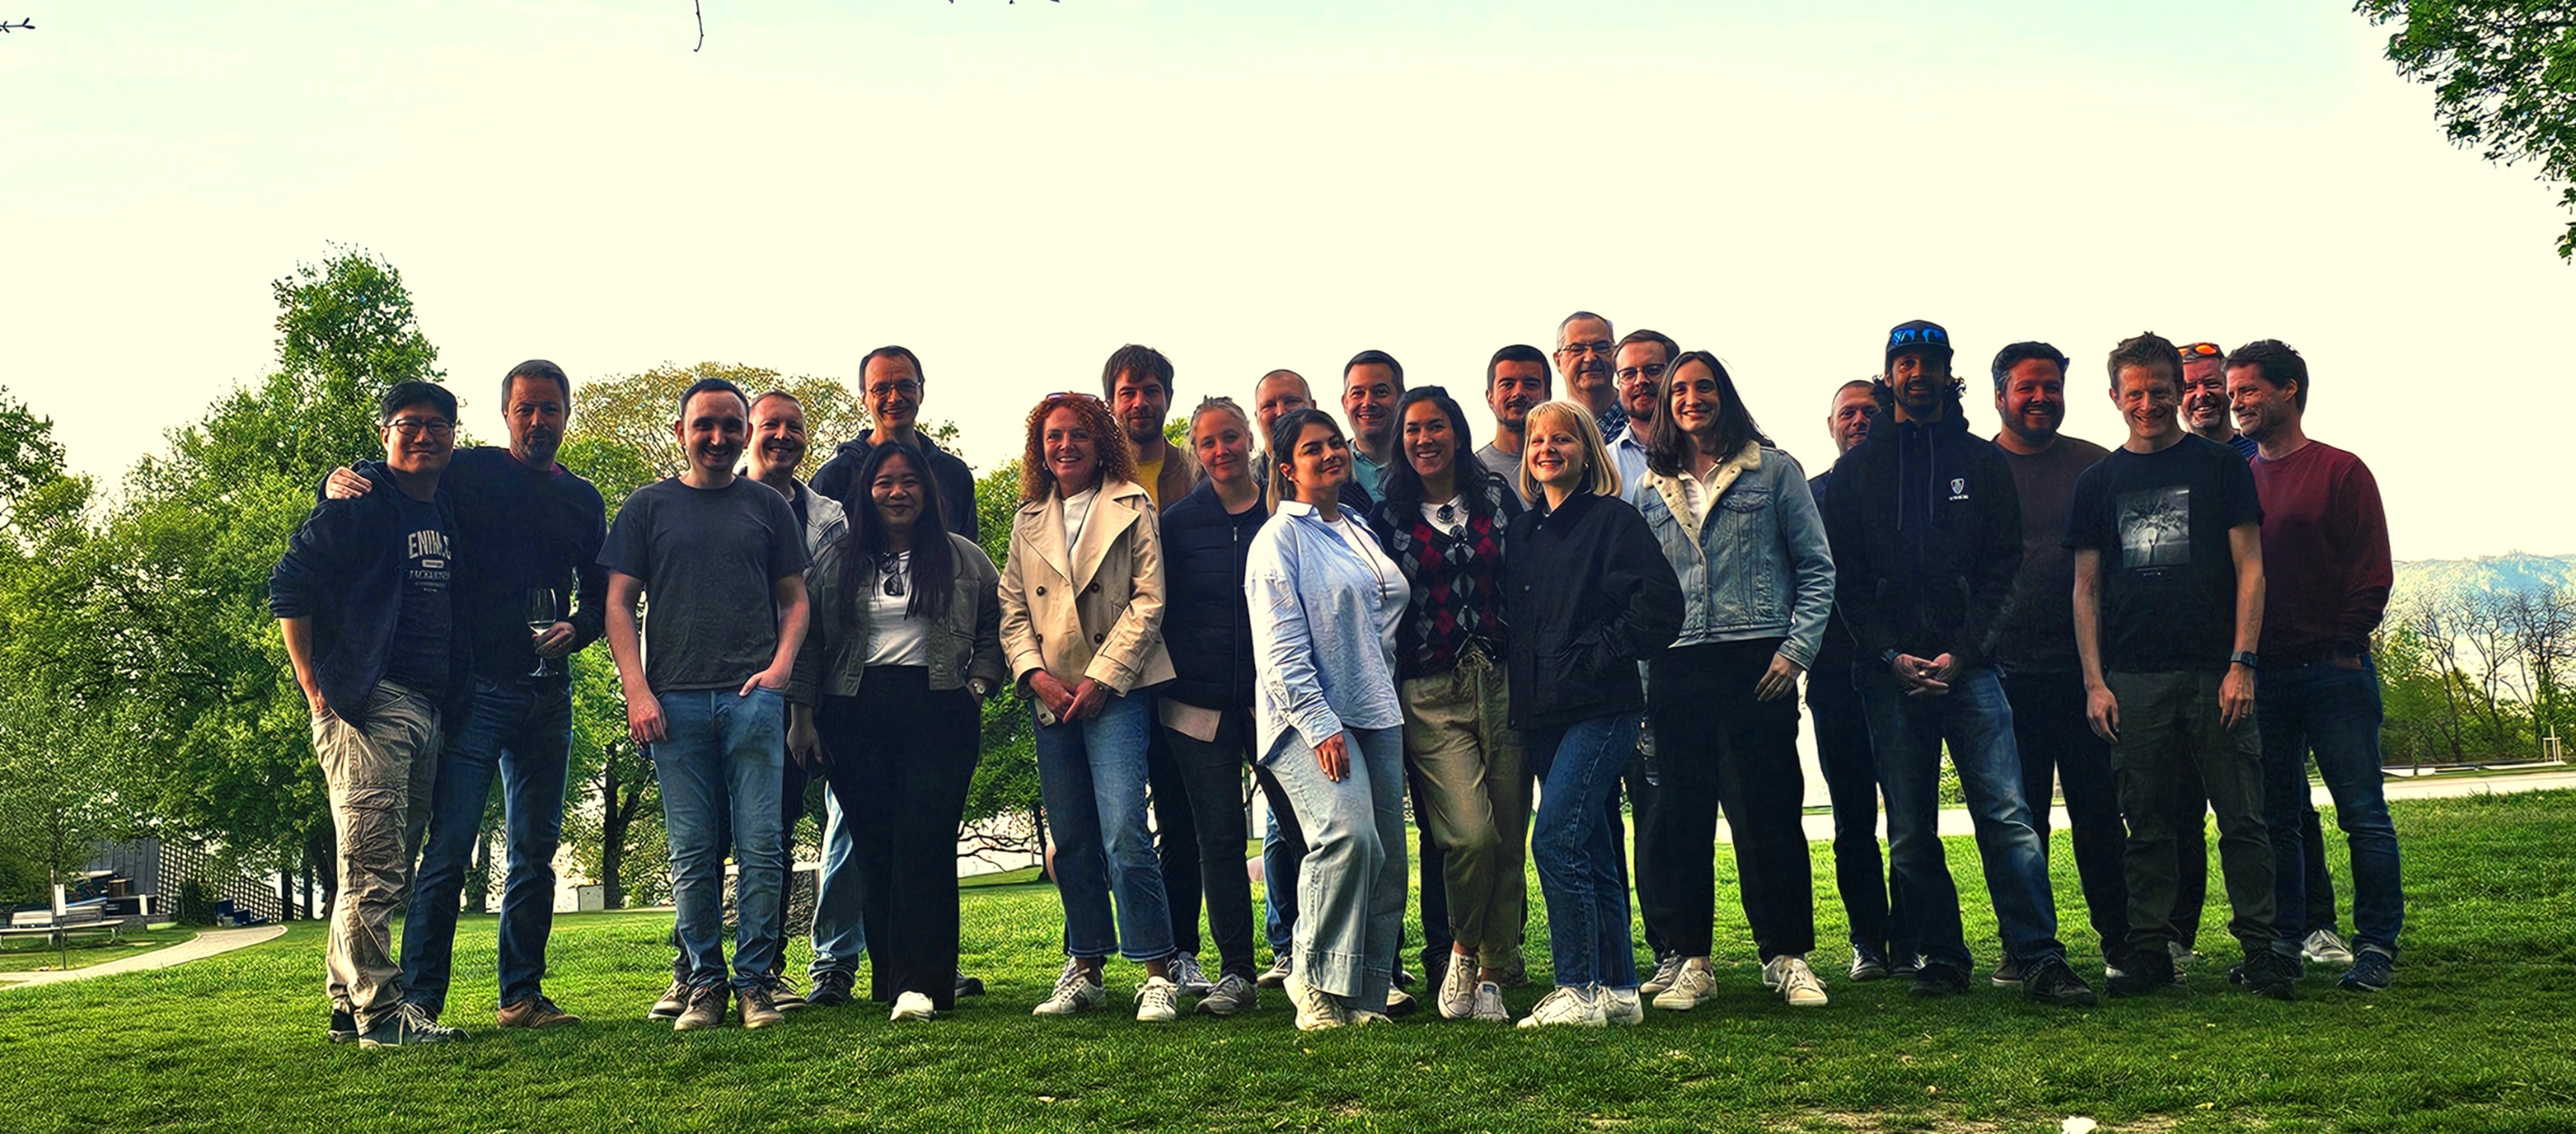
\includegraphics[width=0.8\textwidth]{./content/img/ProjectManagement/BizDevOps_Team.png}
    \caption{Picture of DWH LS OPS team}
    \label{fig:dwhlsops_apero}
\end{figure}

Within the Swiss Post this team is also referred as a \textbf{Busi}ness \textbf{Dev}elopment \textbf{Op}eration\textbf{s} (\gls{BizDevOps})  team, because it contains all required personnel, to create, deploy and maintain reporting solutions. This starts with \gls{businessanalyst}s to evaluate existing reports and their usage, and to document and specify them for further updates or re-engineering. This continues through the implementation, which is carried out first by data engineers and then by business intelligence (\gls{BI}) engineers. Finally, the business side is involved in testing these reports and also serves as the main source when it comes to questions of how or what to implement. Due to the size of this team and the different responsibilities, the DWH LS OPS team consists of three separate sub-teams. These teams are ordered along the process of postal services as introduced in the full mail piece lifecycle being: Receiving, Sorting, Transport, Customs clearance (German acronym is \gls{ASTV}), \textbf{D}elivery \textbf{\&} \textbf{F}inance (\gls{DandF}), and finally the planning focused Parcel Volume Planning and Forecasting (german acronym is \gls{MPP}).

\begin{figure}[H]
    \centering
    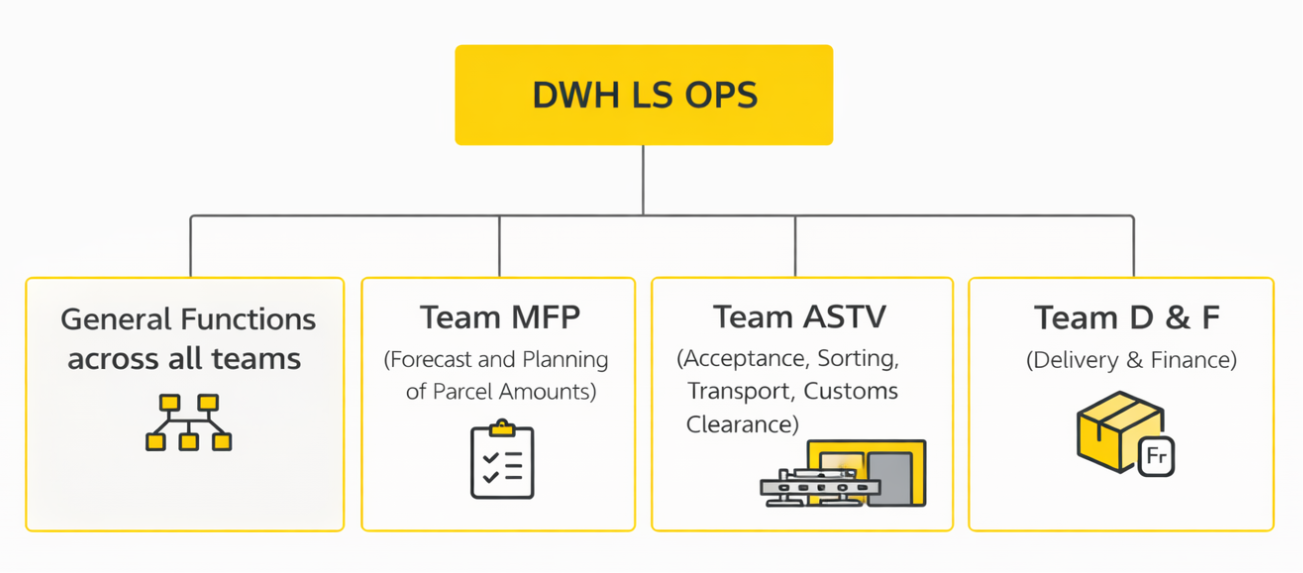
\includegraphics[width=0.8\textwidth]{./content/img/ProjectManagement/BizDevOps_OrgChart.png}
    \caption{Team and sub-team organisation}
    \label{fig:dwhlsops_member_names}
\end{figure}

\subsubsection*{AWS modernisation team}
\label{sec:AWSmodernisationteam}
Swiss Post is currently in a process the modernisation of the AWS cloud environment, which the Swiss Post itself describes as follows:

\textit{Swiss Post is currently pursuing a strategic modernisation of its AWS-based data lake with the objective of improving developer efficiency, increasing operational reliability, and establishing a modern, data-driven architecture. According to internal documentation, the initiative is aligned with defined key performance indicators and aims for completion by the end of the first quarter of 2026 \cite{SwissPostAWSModernization}.}

This modernisation is performed with the assistance of consultants as part of improving AWS usage in DWH LS OPS. The improvements are detailed in 15 \gls{KPI}s across topics such as \gls{AWSGlue} job optimisation and deployment pipeline improvements. With the assistance of the consultants, best practices are applied to the development of \gls{ETL}, as well as general improvements to deployment pipelines. Most importantly for this project, the initiative also includes \gls{DQM} improvements. As a reference, a screenshot of the Confluence landing page describing the initiative is shown below:

\begin{figure}[H]
    \centering
    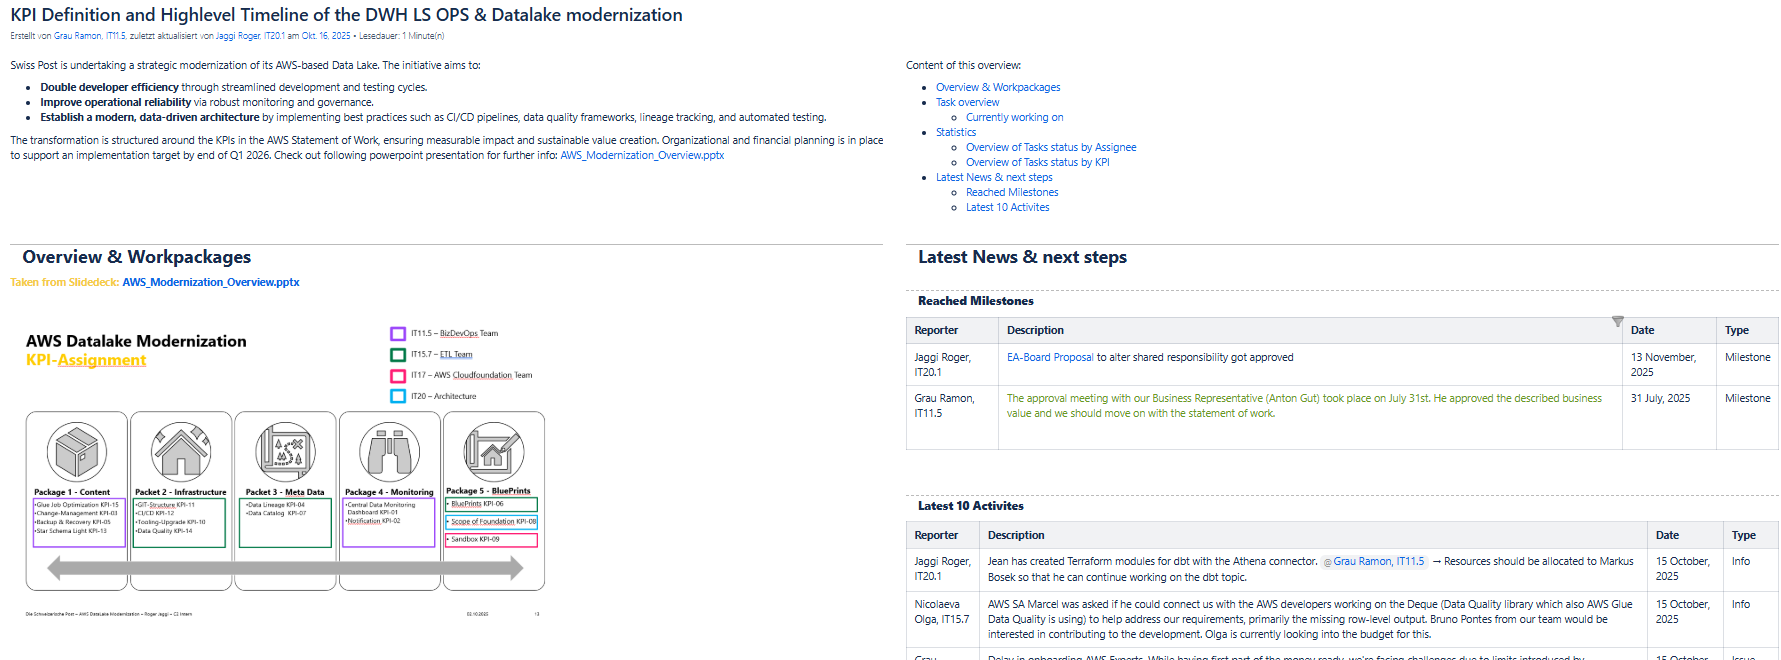
\includegraphics[width=0.8\textwidth]{./content/img/ProjectManagement/AWS_Modernisation_StartPage.png}
    \caption{The start page of the AWS modernisation, listing KPI and latest news}
    \label{fig:aws_modernisation_startpage}
\end{figure}

This team consists mainly of consultants with long-term experience in assisting companies in becoming proficient with AWS. They support data engineers at Swiss Post by improving existing code and reviewing it for potential enhancements. This is relevant for Swiss Post, as the development of the cloud infrastructure started without full architectural support and therefore has room for improvement.

\begin{figure}[H]
    \centering
    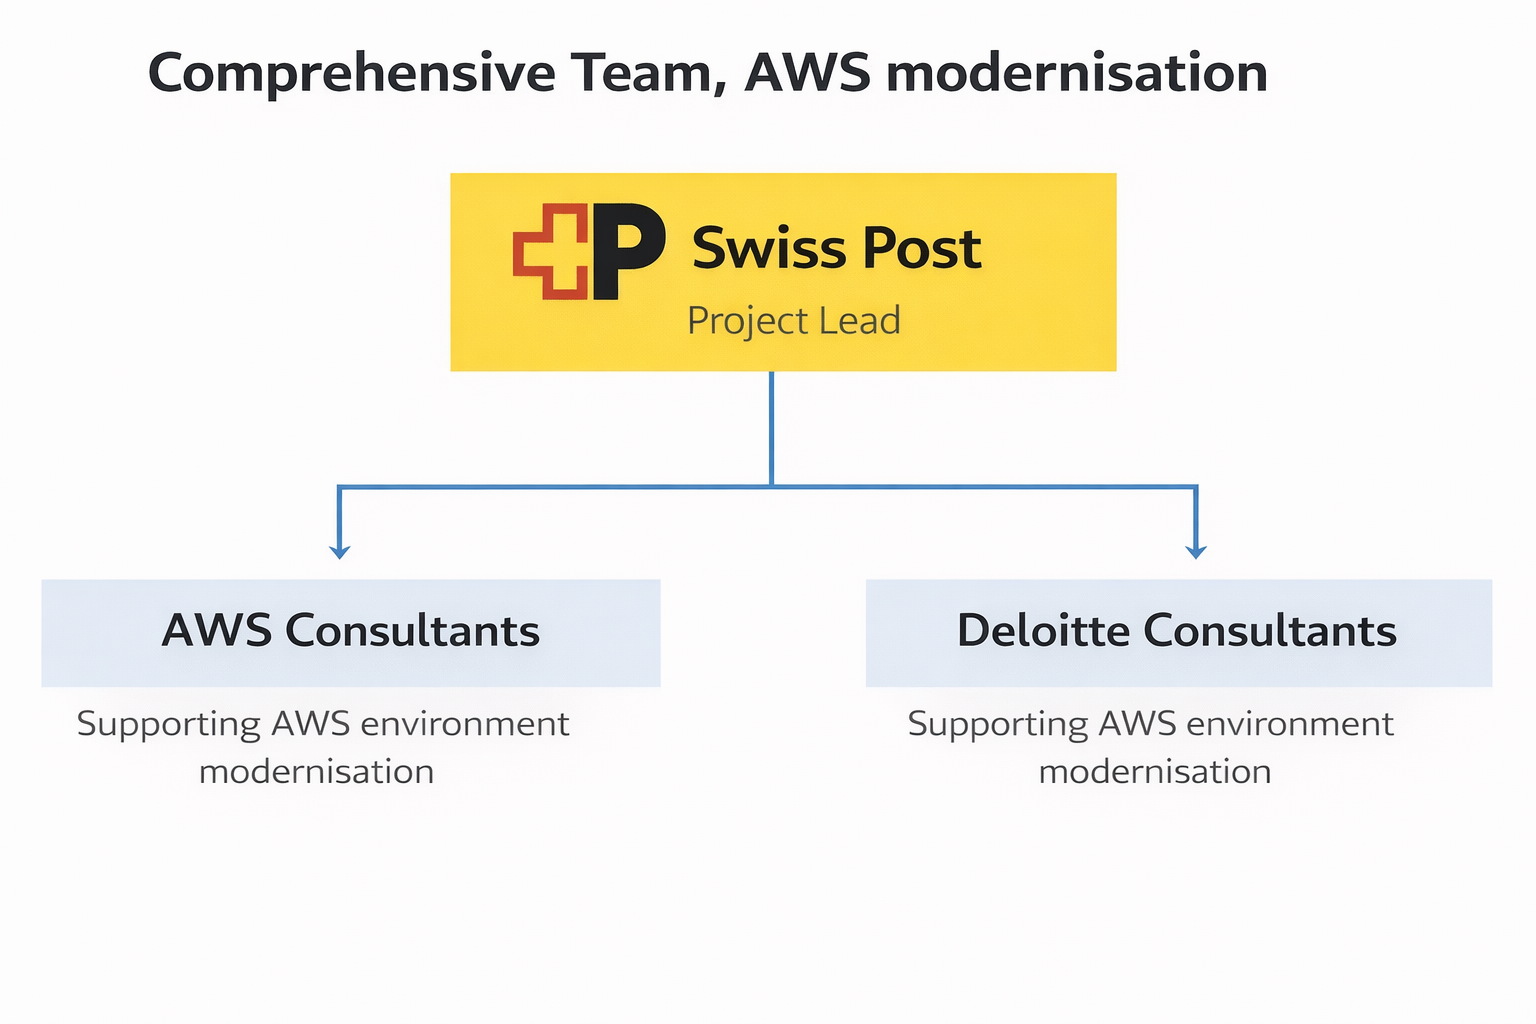
\includegraphics[width=0.8\textwidth]{./content/img/ProjectManagement/AWS_Modernisation_Setup.png}
    \caption{The team setup of the AWS modernisation}
    \label{fig:aws_modernisation_teammembers}
\end{figure}

\subsubsection*{DQM team}
\label{sec:DQMteam}
The third team relevant to the project is the \gls{DQM} team. The team serves KPI 14 Data Quality within the AWS modernisation. Their goal is described on Confluence as follows: specify, review, and implement an MVP to enable data scientists and ETL engineers to forward data quality measures to a monitoring dashboard for both business users and developers.

\begin{figure}[H]
    \centering
    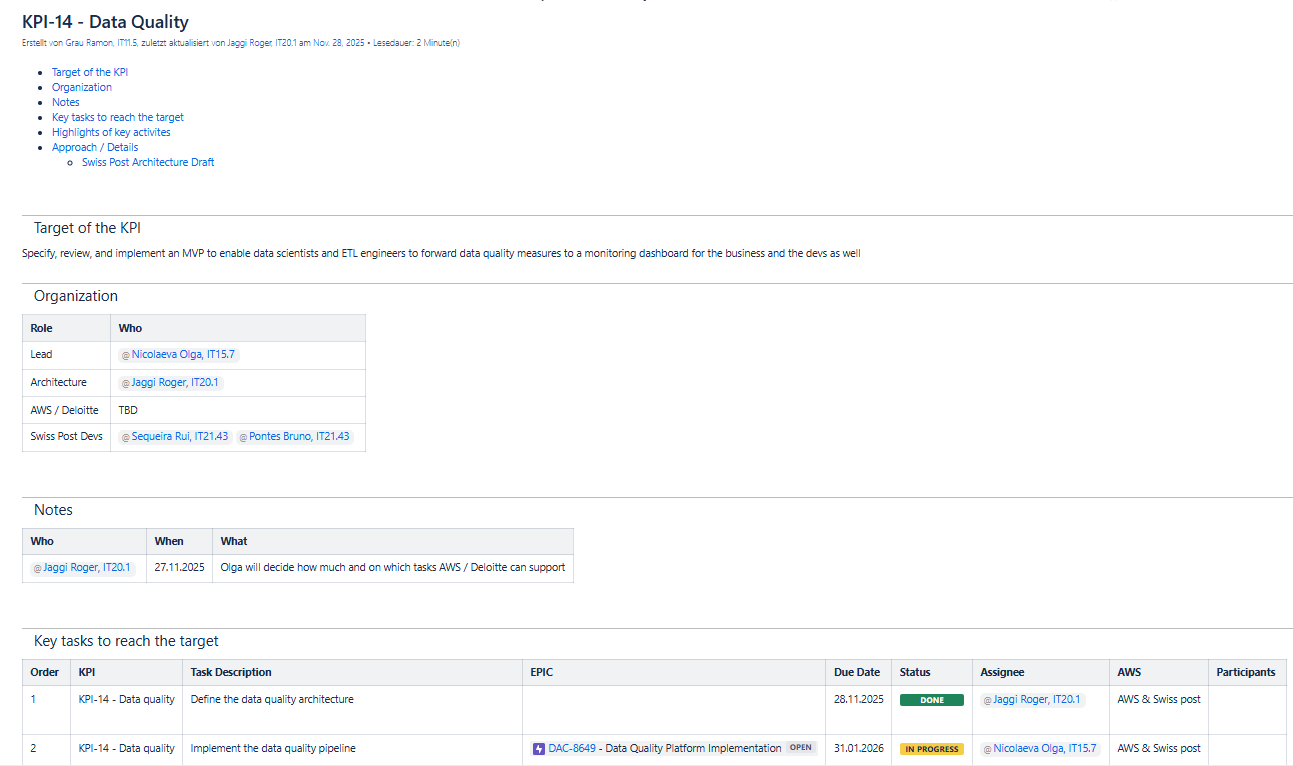
\includegraphics[width=0.8\textwidth]{./content/img/ProjectManagement/Startpage_DQM_KPI14.png}
    \caption{The KPI 14 Data Quality start page on DWH LS OPS Confluence}
    \label{fig:dwhlsops_kpi14_dqm}
\end{figure}

The team consists of three developers with the assistance of a lead data engineer. This setup ensures that the developers can deliver results efficiently, while the lead data engineer provides design guidance and solution structure.

\begin{figure}[H]
    \centering
    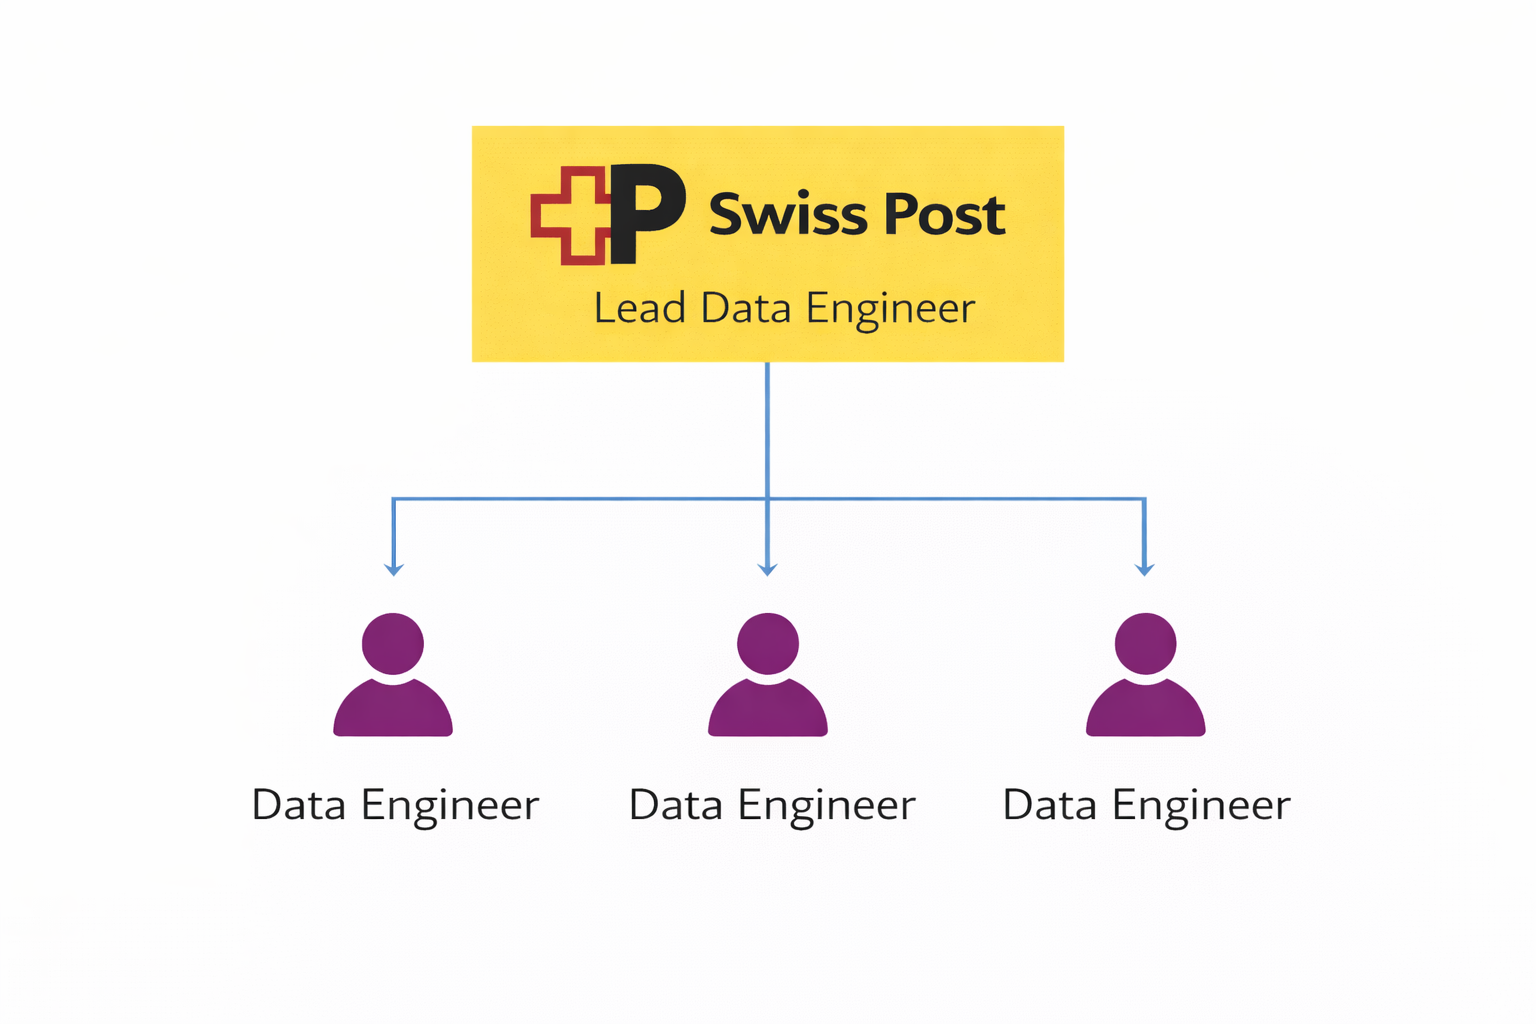
\includegraphics[width=0.8\textwidth]{./content/img/ProjectManagement/DQM_KPI14_Team_NoNames.png}
    \caption{The DQM team setup}
    \label{fig:dwhlsops_kpi14_team_dqm}
\end{figure}

\subsection*{Academic project team}
\label{sec:AcademicTeam}
The academic team consists of the author and the academic advisor. The author conducts the practical work, which includes analysis, implementation, and evaluation. The advisor provides expertise in the academic process and acts as a sparring partner regarding the writing process and project management, offering methodological and academic supervision.

\begin{figure}[H]
    \centering
    
\includegraphics[width=0.8\textwidth]{./content/img/ProjectManagement/ProjectTeam_clean.png}
    \caption{The academic team setup}
    \label{fig:academic_team}
\end{figure}

\section{Project management methodologies}
\label{ProjMgmtMethods}
This section details how the different teams manage themselves. This is done for reasons of transparency, so that the reader understands which project management methods the individual teams use. This highlights an additional level of complexity in the working environment. Not all teams are addressed in every subsection, as the project team was not involved in all teams’ methods to the same depth. First, project management methods are highlighted, followed by the different timeline management approaches. In the following figure, the different boards and management methods are aligned around the central academic team to illustrate the broad set of methods.

\begin{figure}[H]
    \centering
    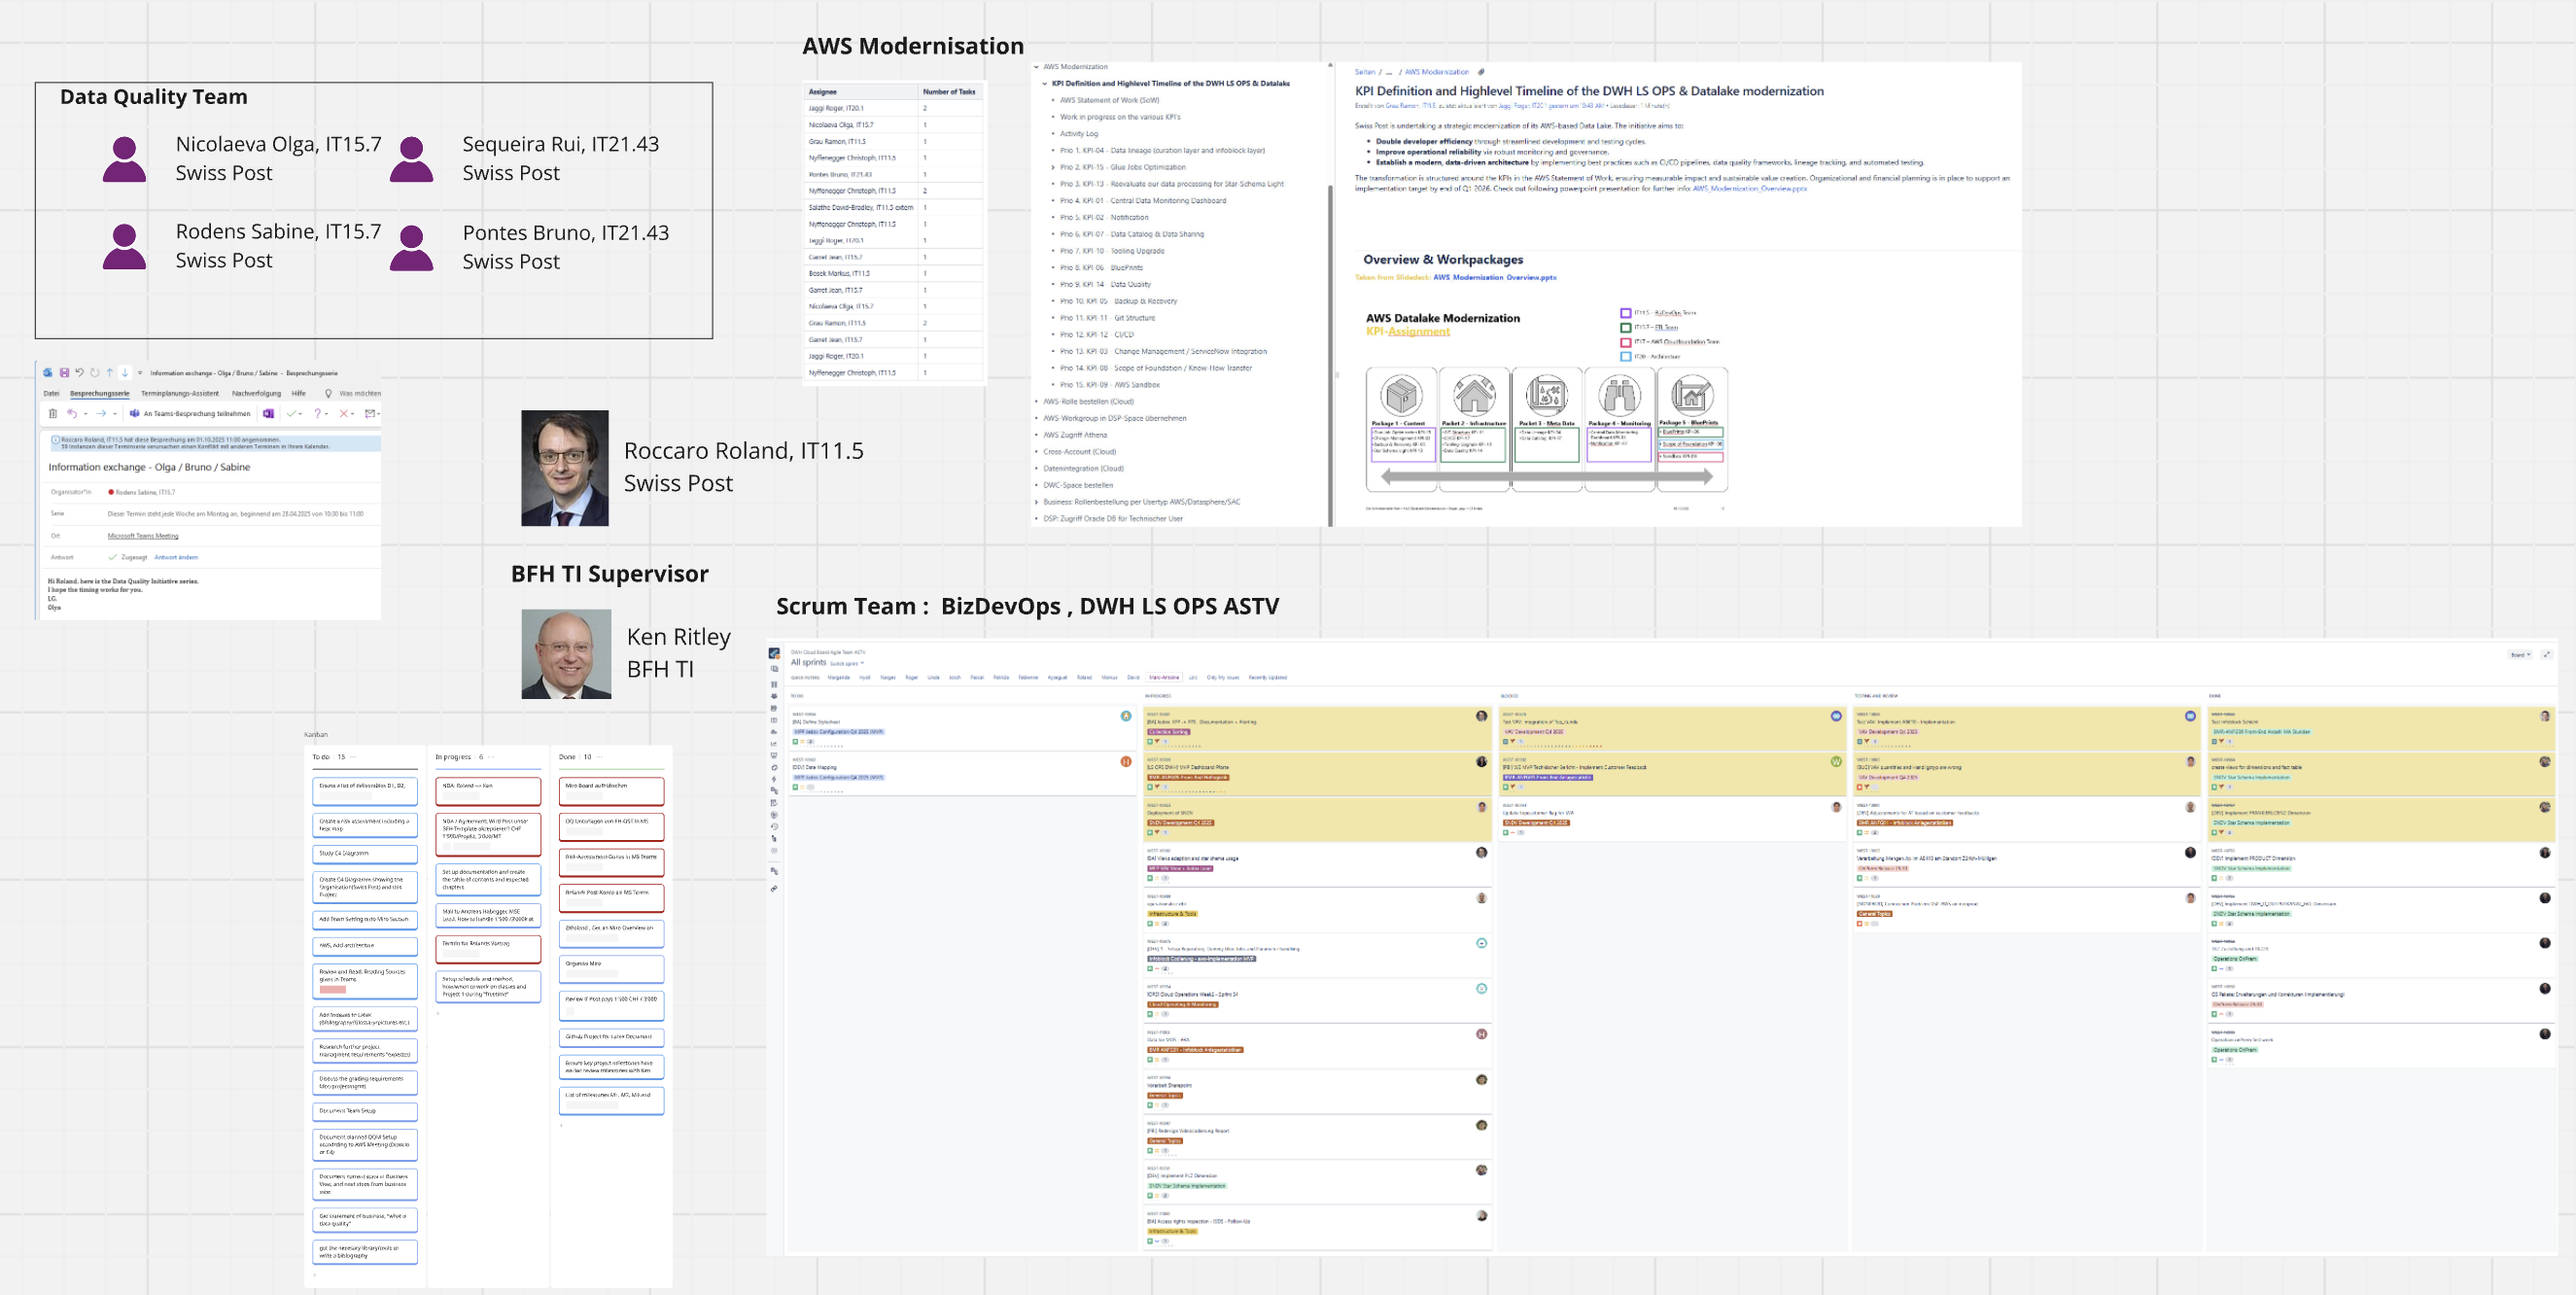
\includegraphics[width=0.8\textwidth]{./content/img/PostTeams_Tools.png}
    \caption{All methods on one picture showing their diversity}
    \label{fig:projmgmt_methods_one_pic}
\end{figure}

\subsection*{Project management}
Project management for this project consists of three main elements. These are Scrum, Kanban, and weekly meetings.

\subsubsection*{Scrum}
The \gls{DWHLSOPS} team is organised as a \gls{BizDevOps} \gls{scrum} team (see Section \ref{sec:DWHLSOPSTeam}). The AWS modernisation teams join these Scrum teams \ref{sec:AWSmodernisationteam}. The full set of rituals defined for Scrum is used, including daily meetings, sprint retrospectives, sprint planning held every two weeks, and reviews held every four weeks. In addition, a weekly Scrum meeting is held to maintain communication between the ASTV, D\&F, and MPP teams. The meetings are shown in the first screenshot, while the second illustrates a noteworthy team definition: the rules of engagement established for collaboration, which are a result of the retrospectives.


\begin{figure}[H]
    \centering
    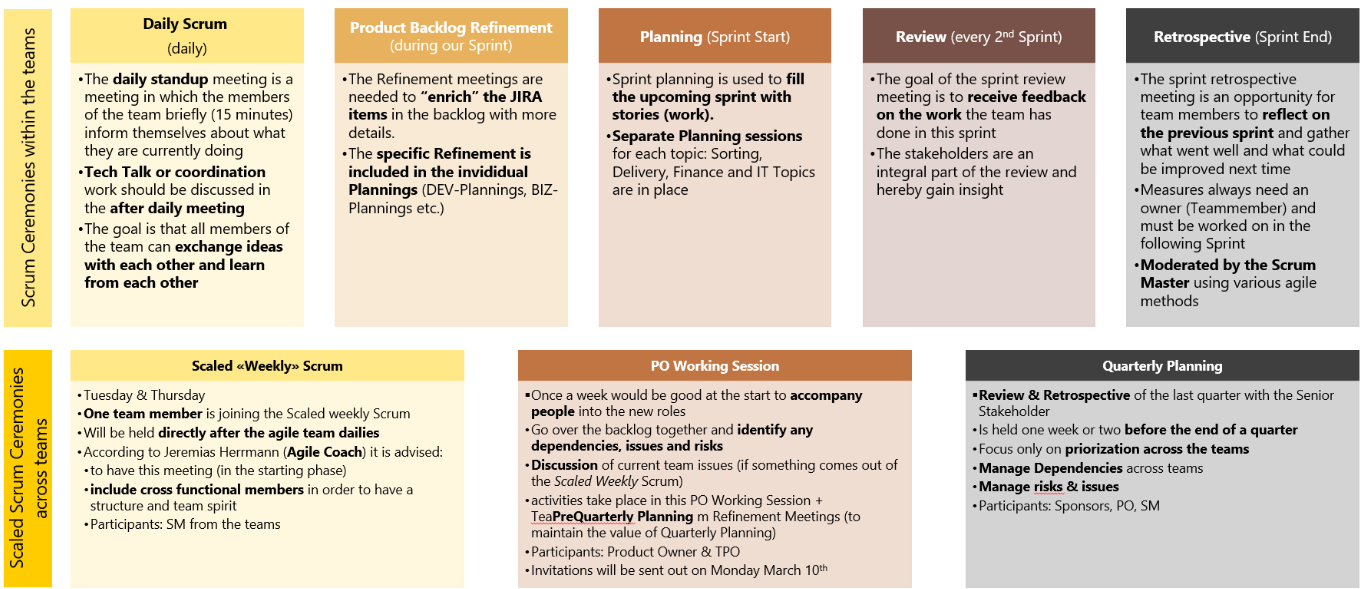
\includegraphics[width=0.8\textwidth]{./content/img/ProjectManagement/BizDevOps_ScrumCeremonies.PNG}
    \caption{Scrum ceremonies of DWH LS OPS  BizDevOps team}
    \label{fig:projmgmt_bizdevops_scrumMeetings}
\end{figure}

\begin{figure}[H]
    \centering
    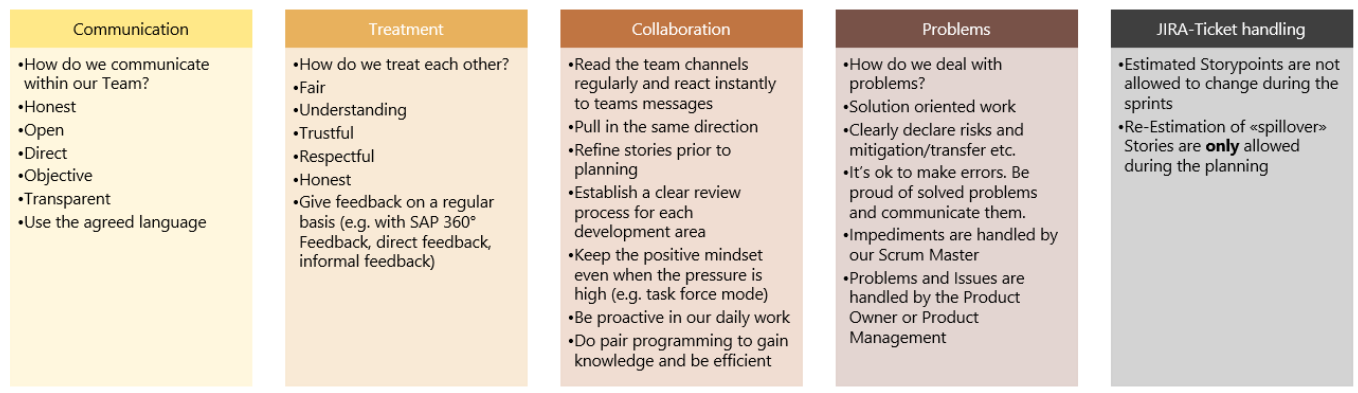
\includegraphics[width=0.8\textwidth]{./content/img/ProjectManagement/BizDevOps_RulesOfEngagement.png}
    \caption{Rules of engagement of DWH LS OPS  BizDevOps team}
    \label{fig:projmgmt_bizdevops_rulesofengagement}
\end{figure}

\subsubsection*{Weekly Meetings}
Contact with the \gls{DQM} team is handled using weekly meetings \ref{sec:DQMteam}. These serve as minimal update sessions during which weekly progress is communicated to all team members. While the developers in the DQM team are themselves also part of a Scrum team, their sprint management is out of scope.

\subsubsection*{Kanban}

The academic team handles tasks using a \gls{kanban} board \ref{sec:AcademicTeam}. The tasks are organised into three main columns. Both team members show their responsibilities on the Kanban board. The blue cards represent the author’s tasks, while the red cards represent the advisor’s tasks. The board is updated frequently and is reviewed during the weekly Jour Fixe.

\begin{figure}[H]
    \centering
    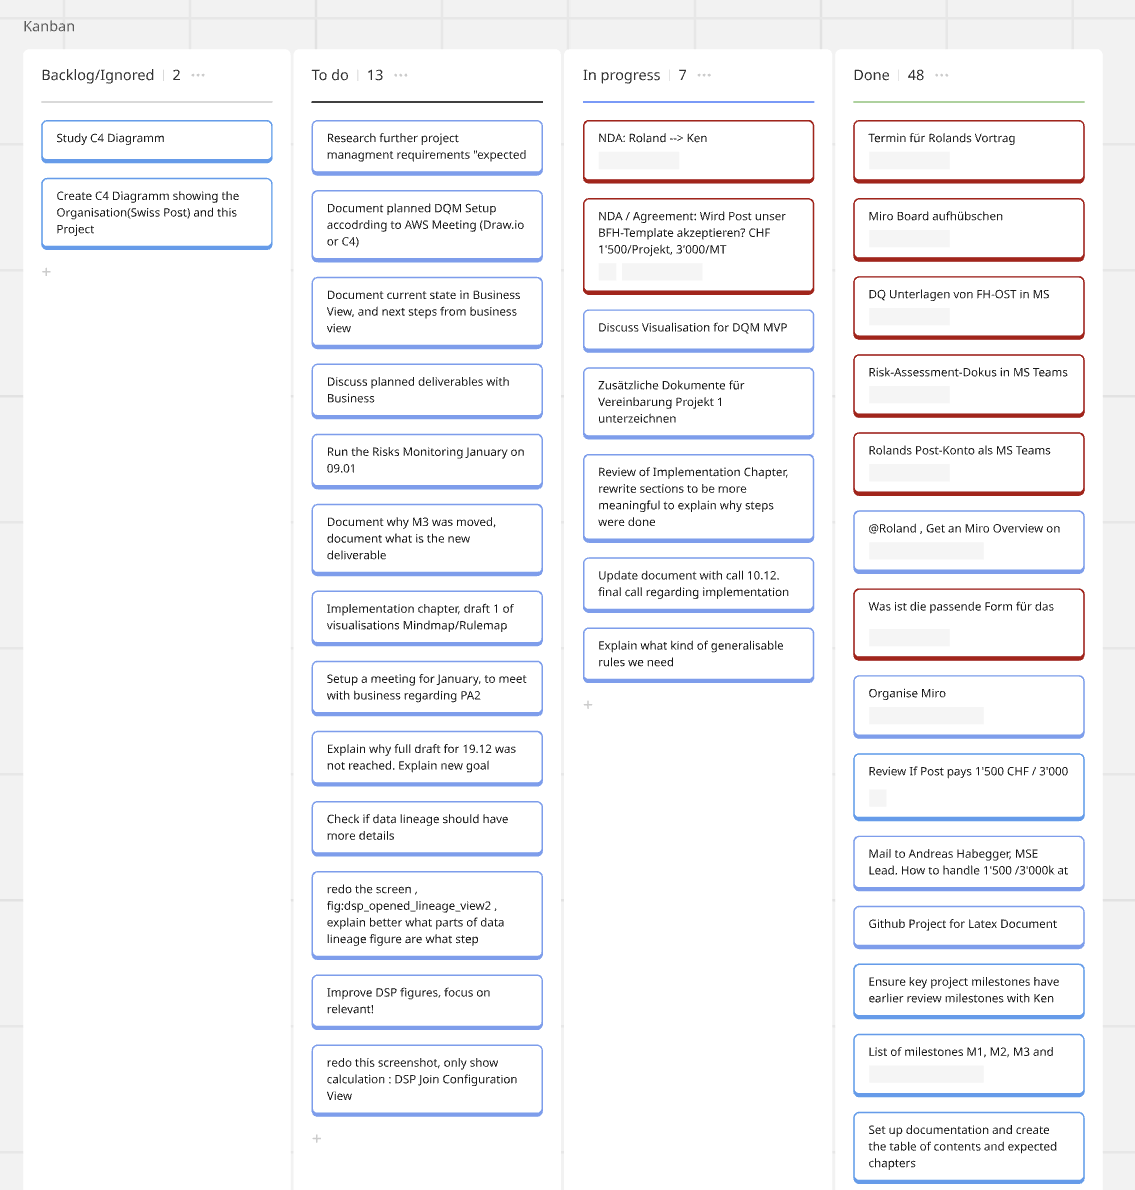
\includegraphics[width=0.8\textwidth]{./content/img/ProjectManagement/Academic_Kanban.png}
    \caption{Kanban board of Academic team}
    \label{fig:projmgmt_academic_kanban}
\end{figure}

\subsubsection*{Jour Fixe}

The academic team holds a \gls{JourFixe} every week \ref{sec:AcademicTeam}. This serves to maintain close communication and functions as a check-up meeting. Each meeting follows a defined structure; as an example, the meeting held on 15.12.2025 is described below.

\begin{itemize}
    \item Project check-in and clarification of objectives
    \item Overview of the project and completed deliverables
    \item Current deliverable in progress
    \item Status of milestones
    \item Changes needed to the updated Project 1 description
    \item Questions regarding Project 2
    \item Other topics
\end{itemize}

First, a general introduction to the project is provided to serve as a check-in and to allow participants to focus on the project. Second, the deliverables currently being worked on are listed based on the deliverables overview. Third, the status of the milestones is reviewed. Fourth, this is followed by individual agenda items, which can differ from meeting to meeting. In this meeting, these included updates to the Project 1 description required for agreement, as well as a check-in regarding topics and submission of Project 2. Finally, the meeting is closed with an open section in which any other relevant topics may be discussed. These meetings are documented in Miro (see below) and structured using a three-block template and are most often recorded using handwritten notes that are later uploaded.


 \begin{figure}[H]
    \centering
    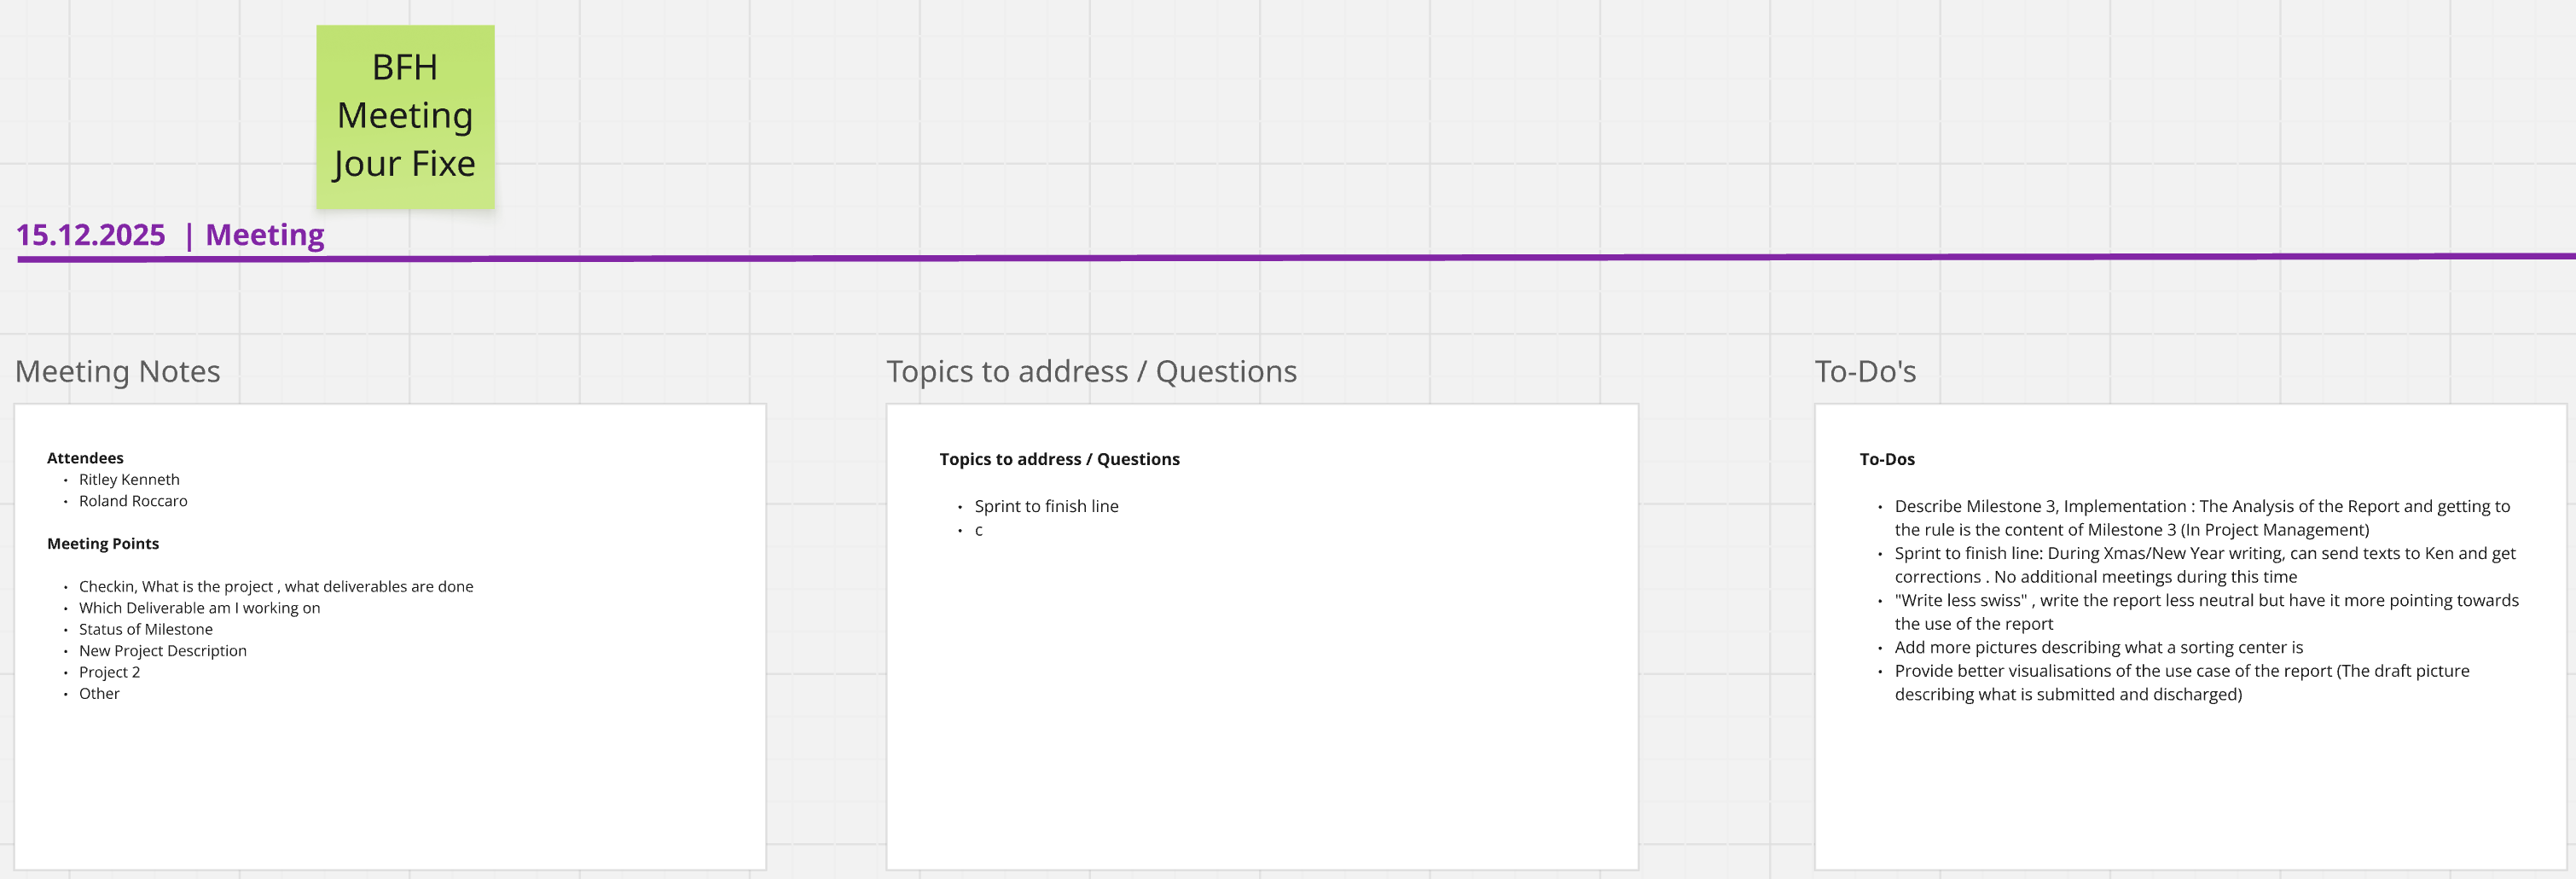
\includegraphics[width=0.8\textwidth]{./content/img/ProjectManagement/Academic_JourFixe.png}
    \caption{Jour Fixe of Academic team, meeting structure and rework}
    \label{fig:jour_fixe_academic_structure}
\end{figure}

\begin{figure}[H]
    \centering
    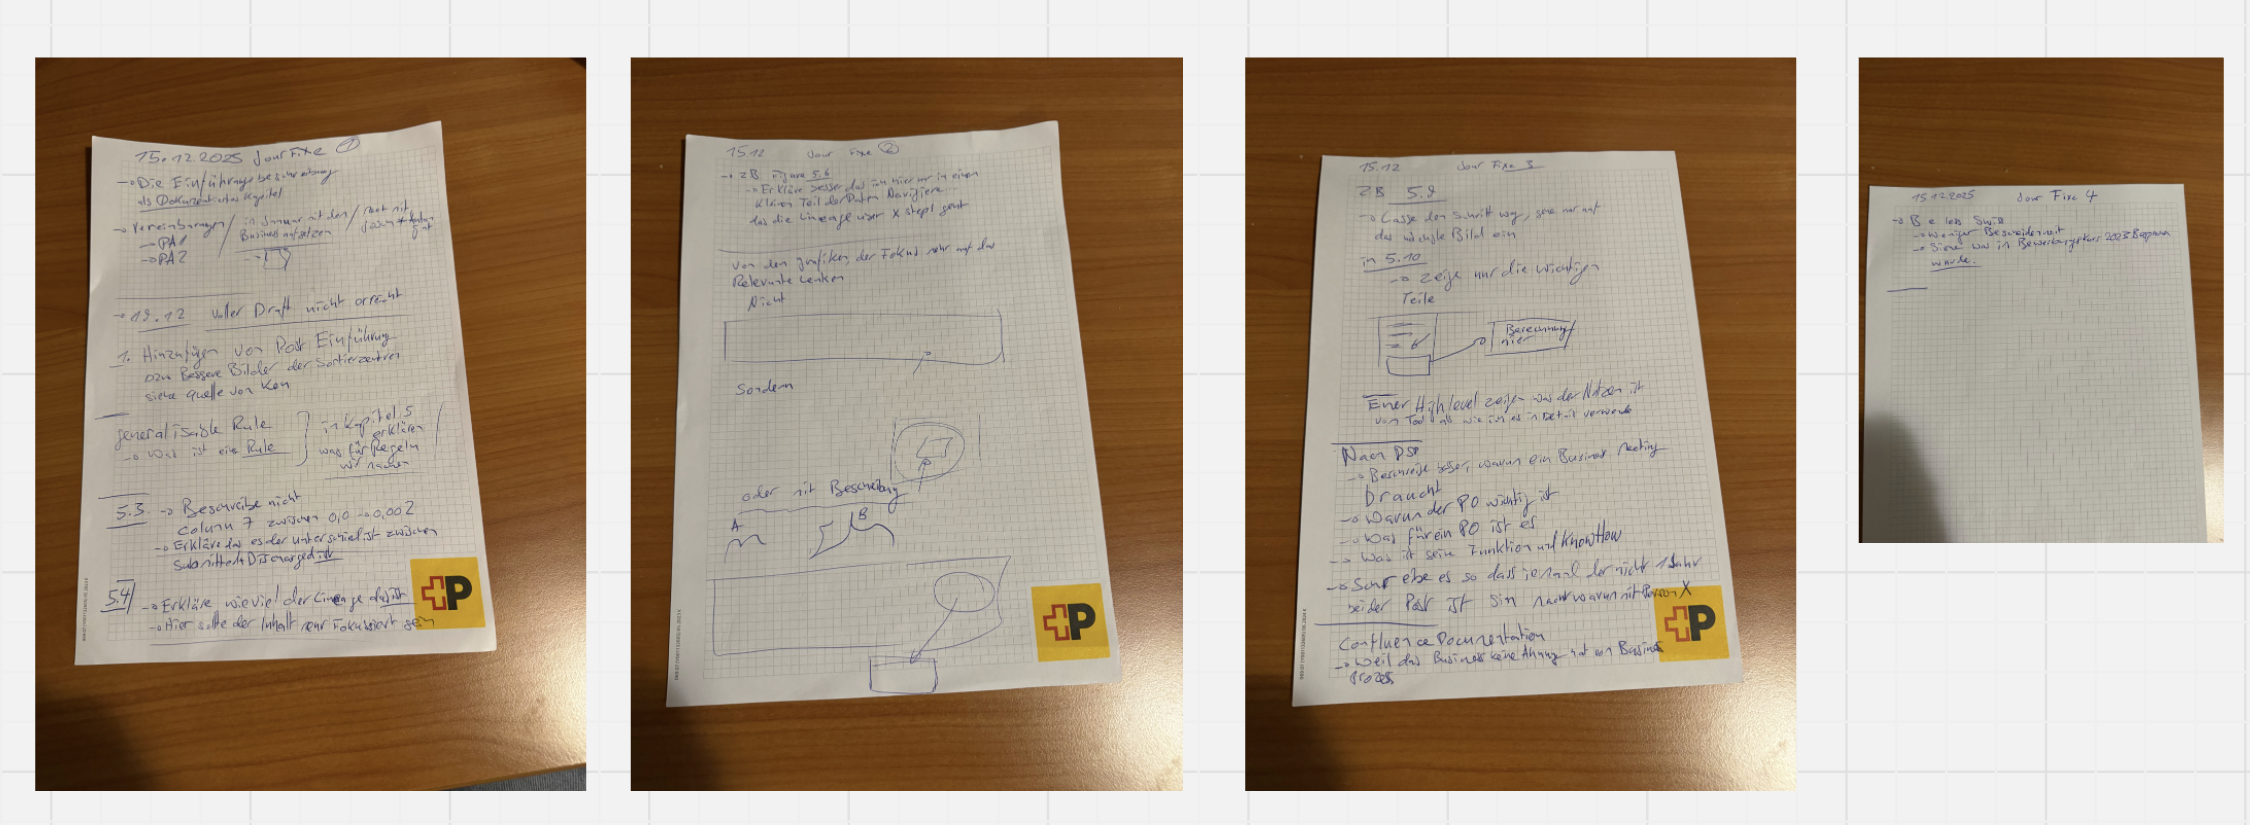
\includegraphics[width=0.8\textwidth]{./content/img/ProjectManagement/Academic_Jour_Fixe_Notes.png}
    \caption{Jour Fixe documentation of Academic team}
    \label{fig:jour_fixe_notes_academic}
\end{figure}

\subsection*{Timeline management}
Timeline management is performed in different ways by the teams. In this subsection, the planning of actions is described, as well as how staff availability is tracked.

\subsubsection*{Scrum Events}
The DWH LS OPS and the AWS modernisation teams use Scrum events to manage their timelines. Progress on stories is monitored in daily meetings, during which each team member updates the team on progress and issues and indicates whether assistance is needed or deviations from the previously planned approach are required. Sprints encompass the stories the team works on during a two-week cycle. During sprint planning, the stories for the next sprint are defined. The stories added to a sprint represent the commitment the team makes for the sprint, together with the sprint goal. Planning over longer time horizons is conducted through quarterly planning sessions. Every three months, all teams in DWH LS OPS plan which \gls{epic}s and how many story points should be completed. These quarterly planning sessions also serve to prioritise epics and allow higher management to introduce priorities.

\subsubsection*{Holidays}
Holidays are noted in the calendars used; this applies to the DWH LS OPS team as well as the academic team. In both cases, every holiday must be recorded with an absence notification. This allows other team members to quickly see whether a team member is available in the future and to adjust their planning accordingly, or to confirm in daily operations that the person is not available.

\subsubsection*{Milestones}
The academic team manages the planning of the overall project timeline using milestones. These milestones define timeframes during which a section or chapter may be worked on. For this project, the following milestones have been defined:

\begin{itemize}
    \item Milestone 1: Basics completed
    \item Milestone 2: Completion of main research
    \item Milestone 3: Code implementation completed
    \item Milestone 4: Bug fixing completed
    \item Milestone 5: Submission of the project document
    \item Milestone 6: Presentation prepared
\end{itemize}

First, the basics ready refers to tools to work with beeing available. This step includes setting up LateX, setting milestones, setup of basic tool structure and definition of way of work. Second the main research done refers to the end of the purely theoretical part and start towards the solution design and the subsequent implementation of it. This comprises the main literature research beeing done. Third, the code done refers to the implementation of the solution beeing done. After this point no new features are to be implemented. Fourth, bug fix done comprises all corrections that had to be performed so that the provided implementation works and technical debt amassed during development has been cleared. Fifth, the handin of the document is the final day according to the semester calender. Up to this date corrections to the document and finalisation can be provided. Sixth and final, the presentation must be ready latest by this date. After this some finetuning can be performed but the main content needs to be set.

The milestones were set to structure the work blocks, but primarily to define how much effort should be invested in each individual block. The time allocated per block is not estimated in terms of how long a task is expected to take. Instead, it is defined by how much time the team is willing to invest in a topic in order to ensure sufficient capacity for subsequent tasks. For example, documenting the Swiss Post environment could have taken two to three weeks; however, only three days were intentionally allocated to this task.

\subsubsection*{Deviations and Unavailabilities}
The academic team tracked deviations from milestones or Jour Fixe meetings. This served transparency and traceability. For this use case, the dates of all Jour Fixe meetings were planned in advance. If a meeting had to be rescheduled, this was noted in the calendar. In the case of shifted milestones, these changes also had to be documented in the calendar, including the reasoning for why a milestone was not achieved or had to be moved. In the Results chapter, deviations from the planned milestones are documented.
\section{Tools to support the project management}
\label{ProjMgmtTools}
This section lists the tools used during the project for reasons of transparency. It also allows the reader to evaluate different ways in which these tools can be used. 

\subsection*{Miro}
\label{ProjMgmtToolMiro}
Miro is part of the toolset of both the academic team and the Swiss Post teams. However, in this project, it was used only by the academic team. The reason for using Miro is that it is a lightweight tool that allows combining different data structures on a single board. Miro provides an infinite canvas on which a wide variety of information can be placed. The information can be structured and easily rearranged to regroup related elements. This allows the tool to be used both for early documentation of information and for later restructuring when additional ideas emerge, particularly in the context of long-term documentation. The ability to restructure information visually supports the decomposition and understanding of complex environments.

A full set of screenshots illustrating changes on the Miro board has been moved to the Annex, while the final one is included here (Appendix \ref{apendixMiroUsage}). The following screenshot represents the Miro board during the finalisation of the document, zoomed out so that all elements are visible. While this view prevents individual details from being seen, some relevant parts are shown in detail in the following subsubsections.

\begin{figure}[H]
    \centering
    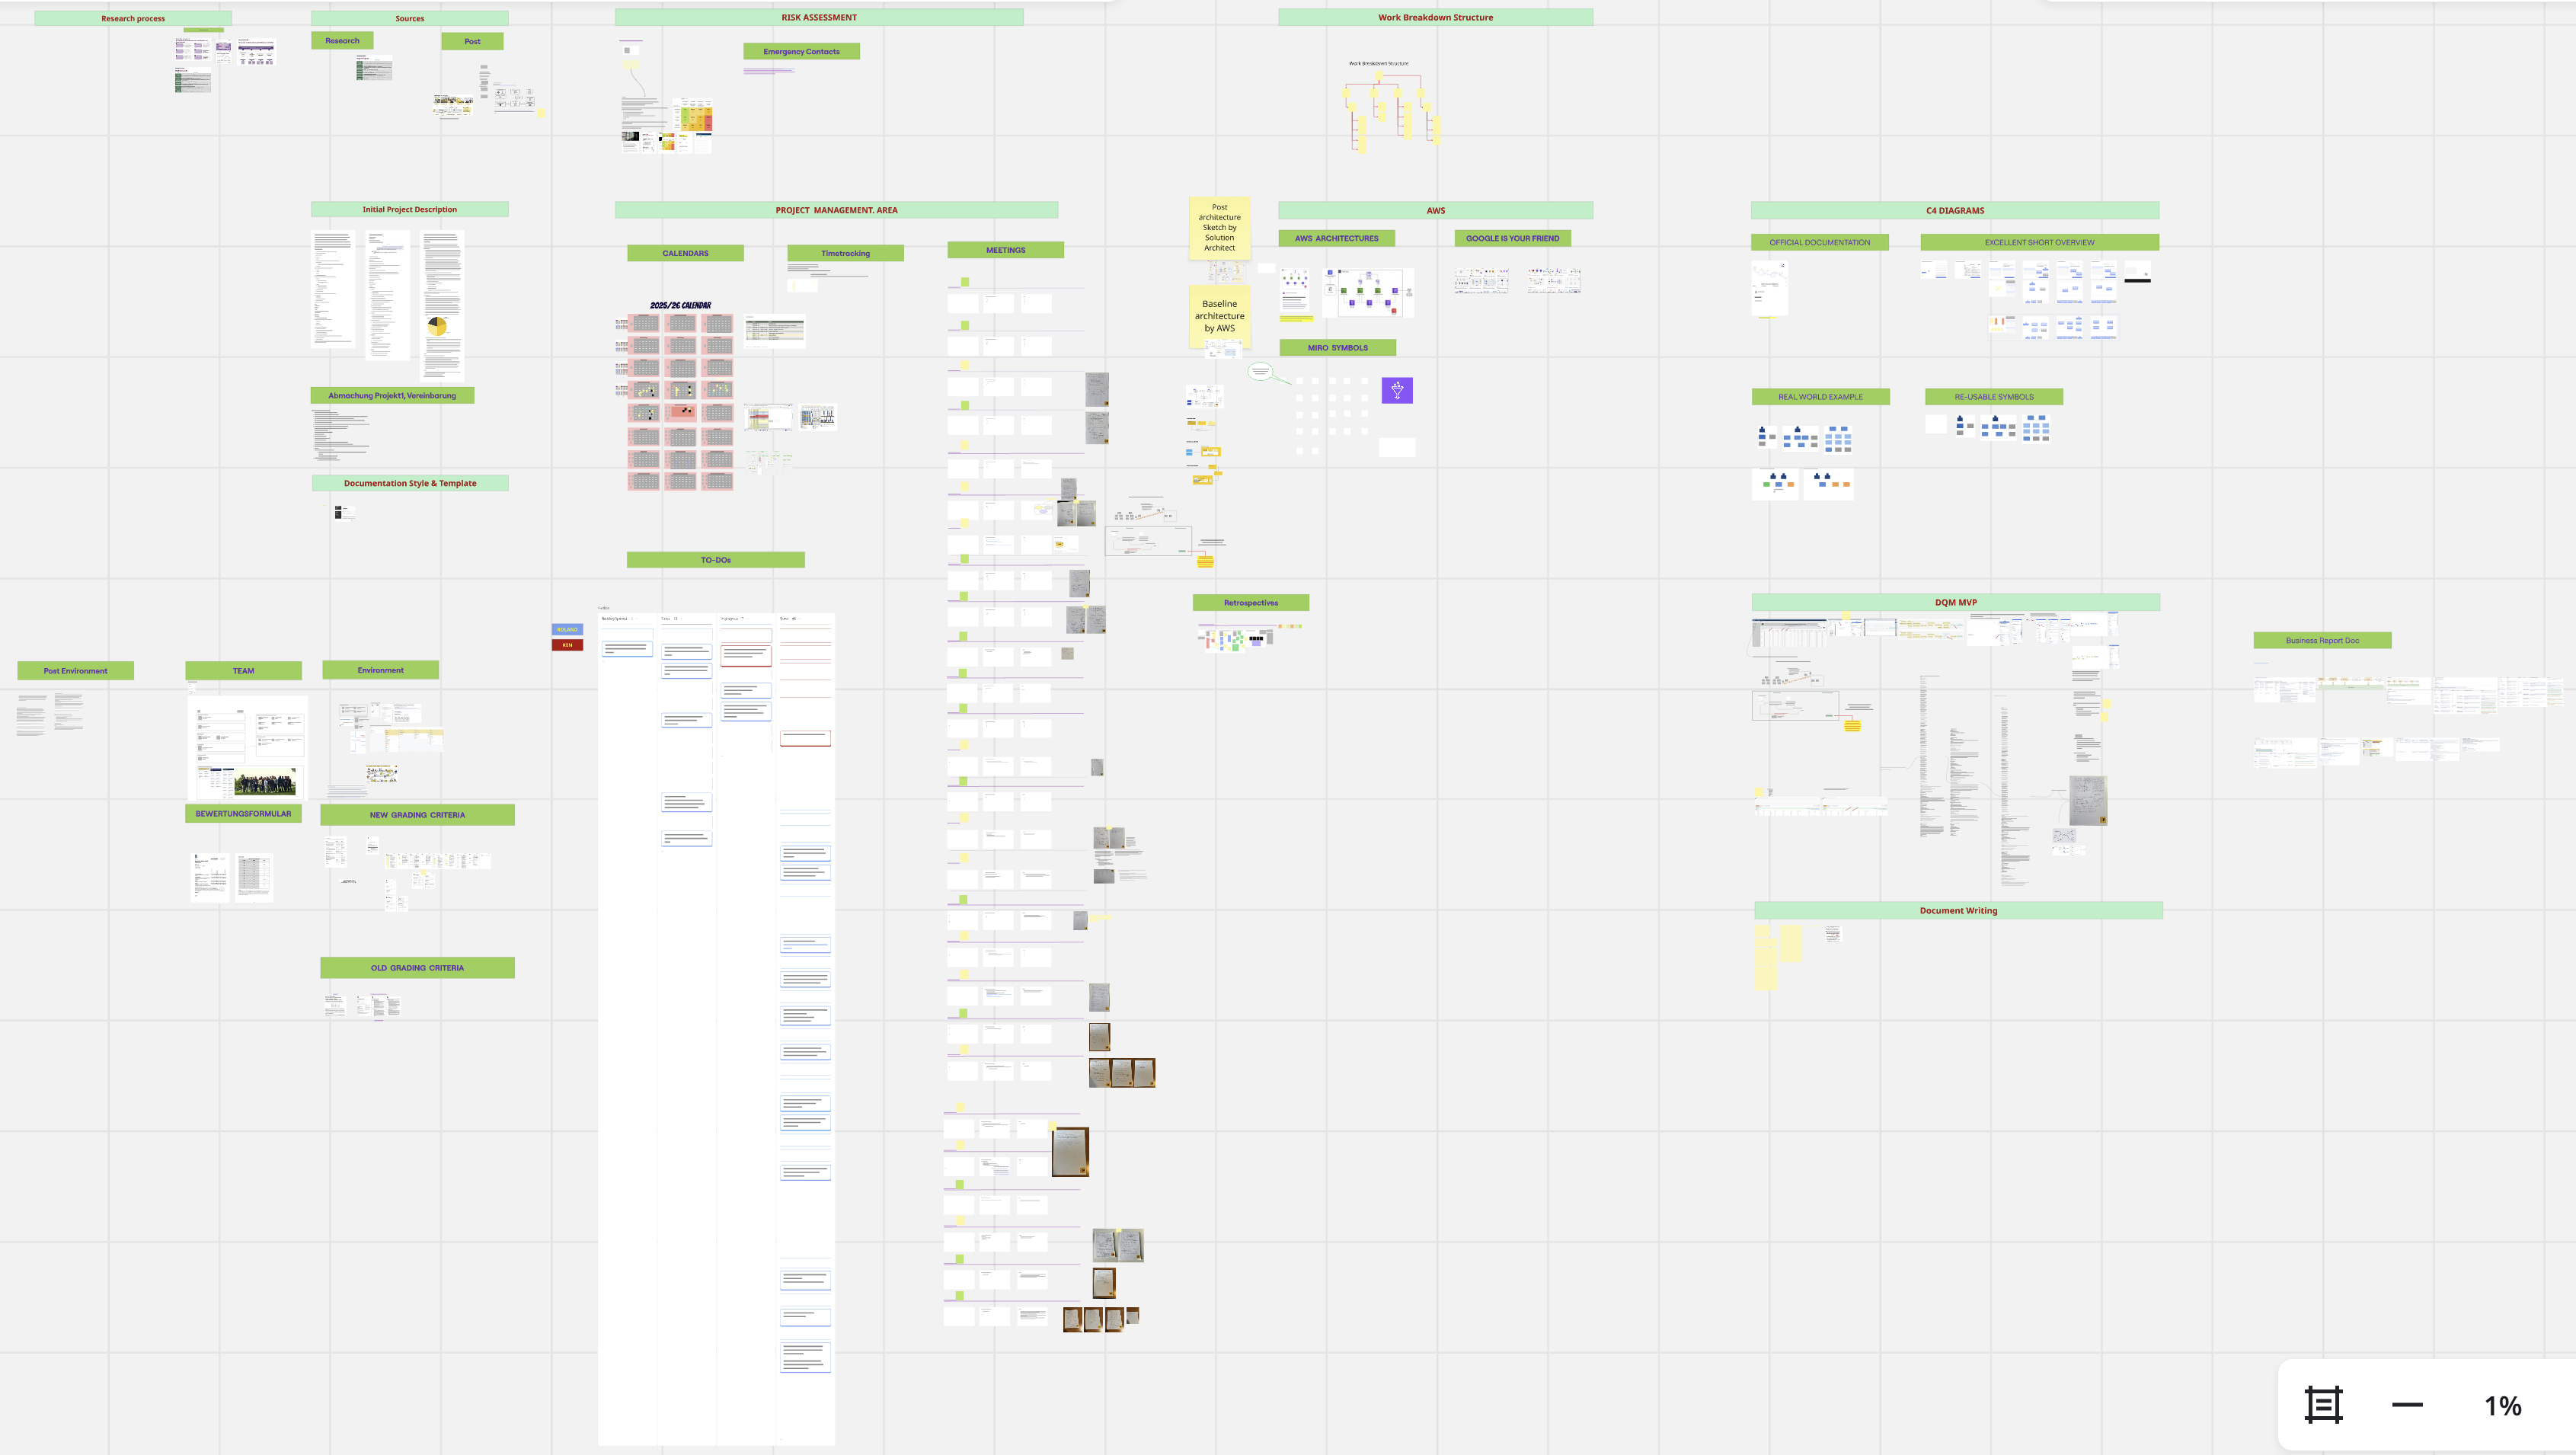
\includegraphics[width=0.8\textwidth]{./content/img/MiroBoard_23-12-2025.png}
    \caption{Miro board documentation, view of 23.12.2025}
    \label{fig:miro_final_board_twentythird_december}
\end{figure}

\subsubsection*{Miro calendar}
The calendar in Miro was primarily used to schedule the milestones. These are shown with green tiles on the corresponding dates, including their number and milestone title. Jour Fixe meetings are marked in yellow whenever they occurred, including adjustments in cases of unavailability. Actual unavailabilities at scheduled Jour Fixe meetings and other times are documented in black. Finally, holidays are marked in teal. In the case of this project, this applied only to the Christmas and New Year holiday period.

\begin{figure}[H]
    \centering
    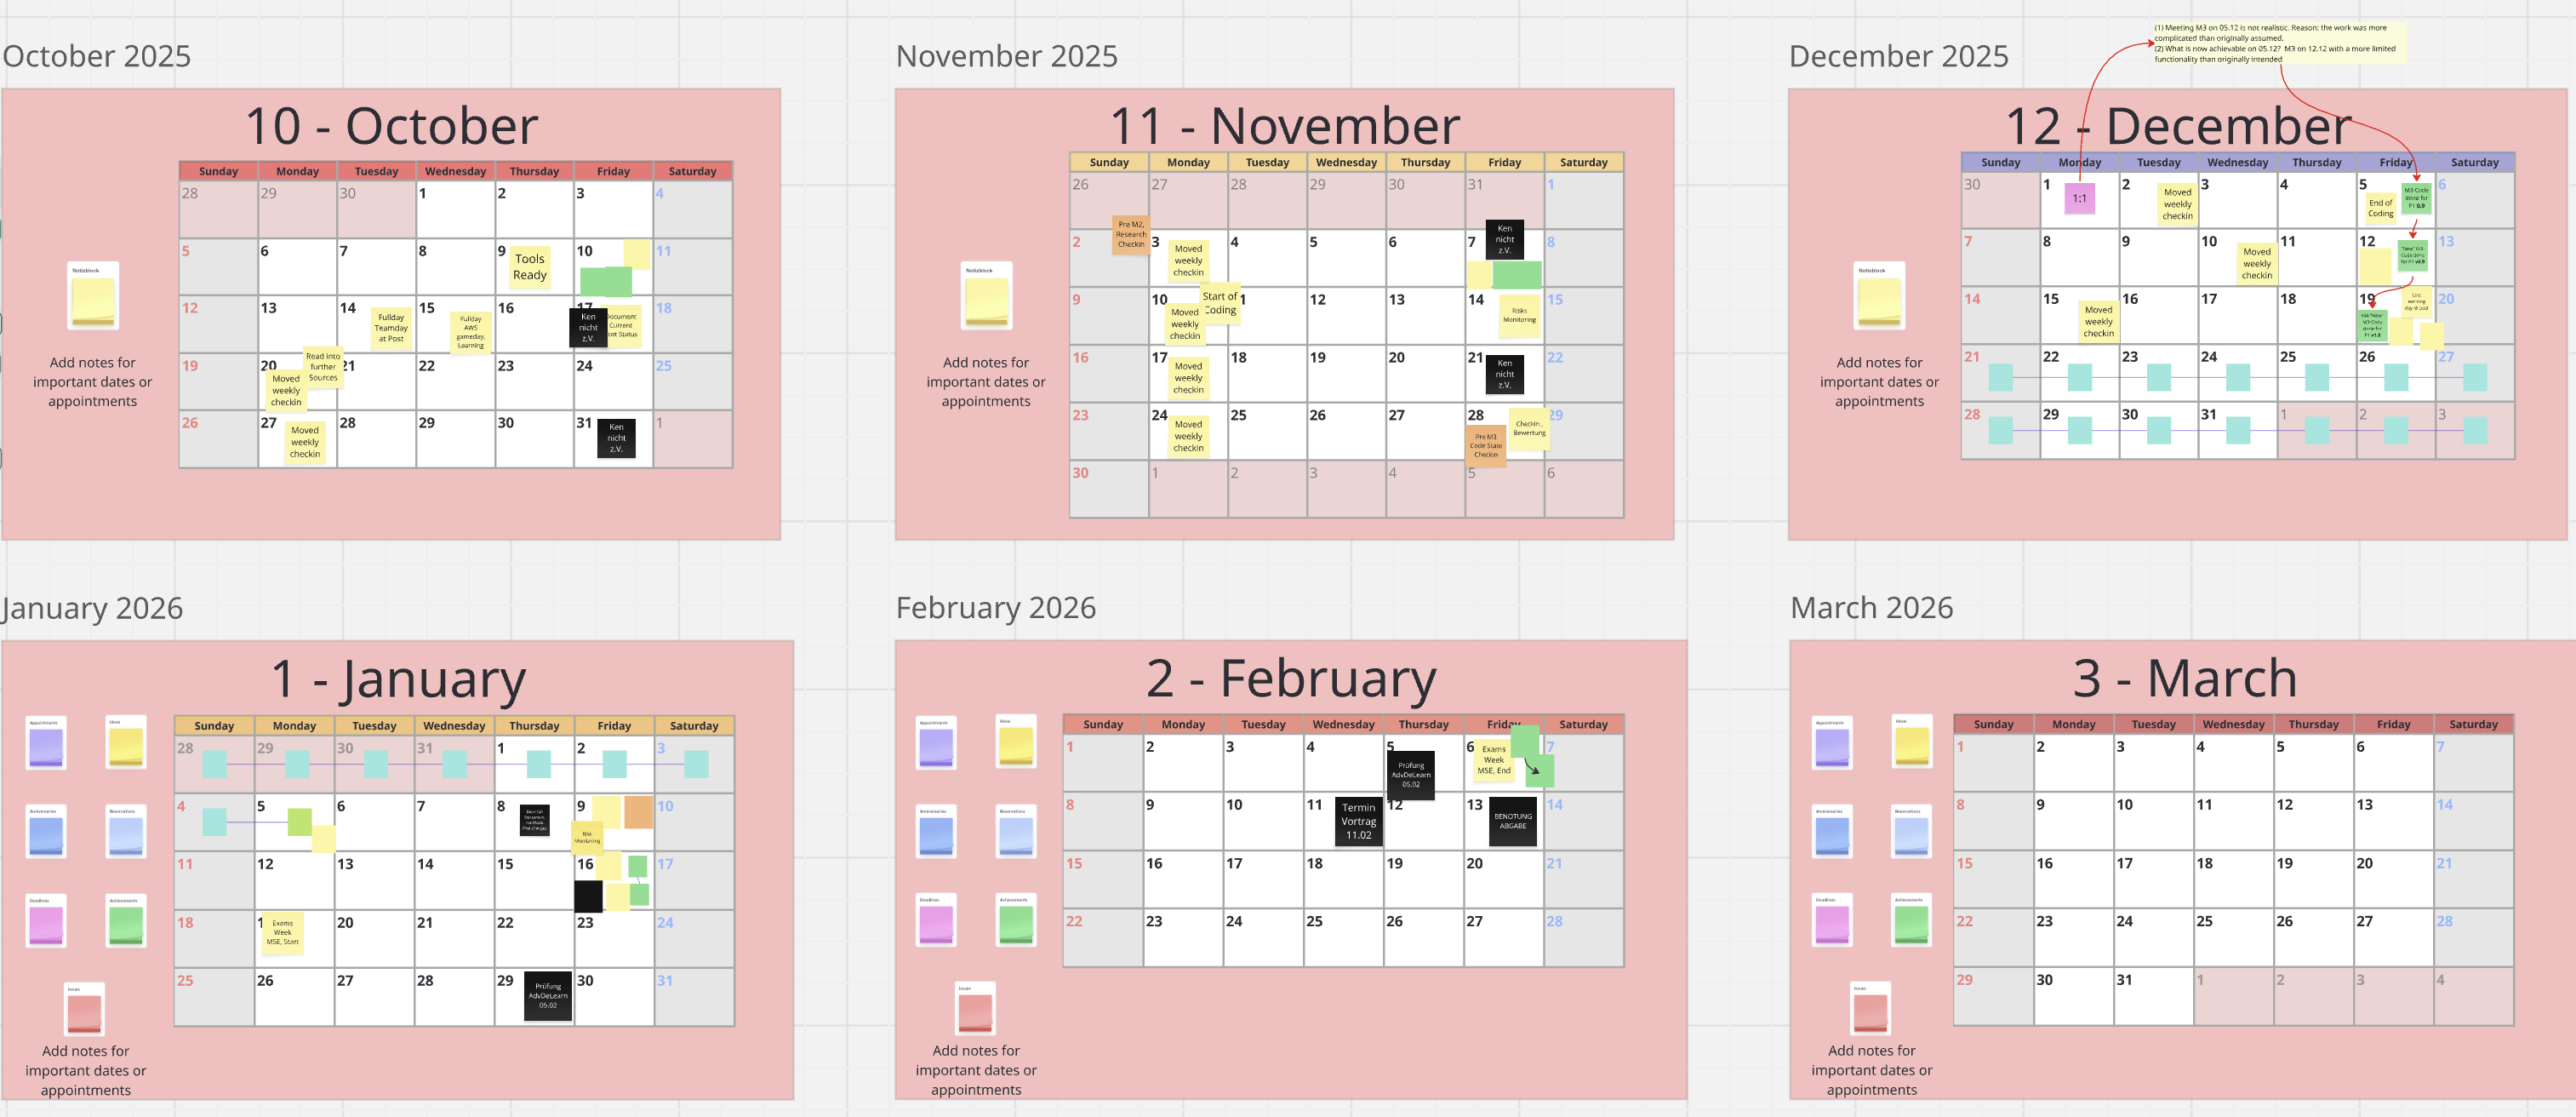
\includegraphics[width=0.8\textwidth]{./content/img/MiroBoard_Calendar.png}
    \caption{Miro board calendar used for coordination and tracking of milestones and related events}
    \label{fig:miro_board_calendar}
\end{figure}

\subsubsection*{Meetings documentation}
The meetings are documented using a layout with three sections, including a coloured tag at the top in yellow for Swiss Post meetings and green for academic ones. From left to right, these sections are structured as follows. First, the meeting points to be discussed are listed; these are copied from the Outlook invitations. Second, the topics addressed are summarised, mostly after the meeting. Third, the to-do block describes any actions that arose during the meeting. Not every meeting includes all sections. Furthermore, meetings are often documented using handwritten minutes. These are uploaded to the right of the meeting blocks without further refinement and serve as references.

\begin{figure}[H]
    \centering
    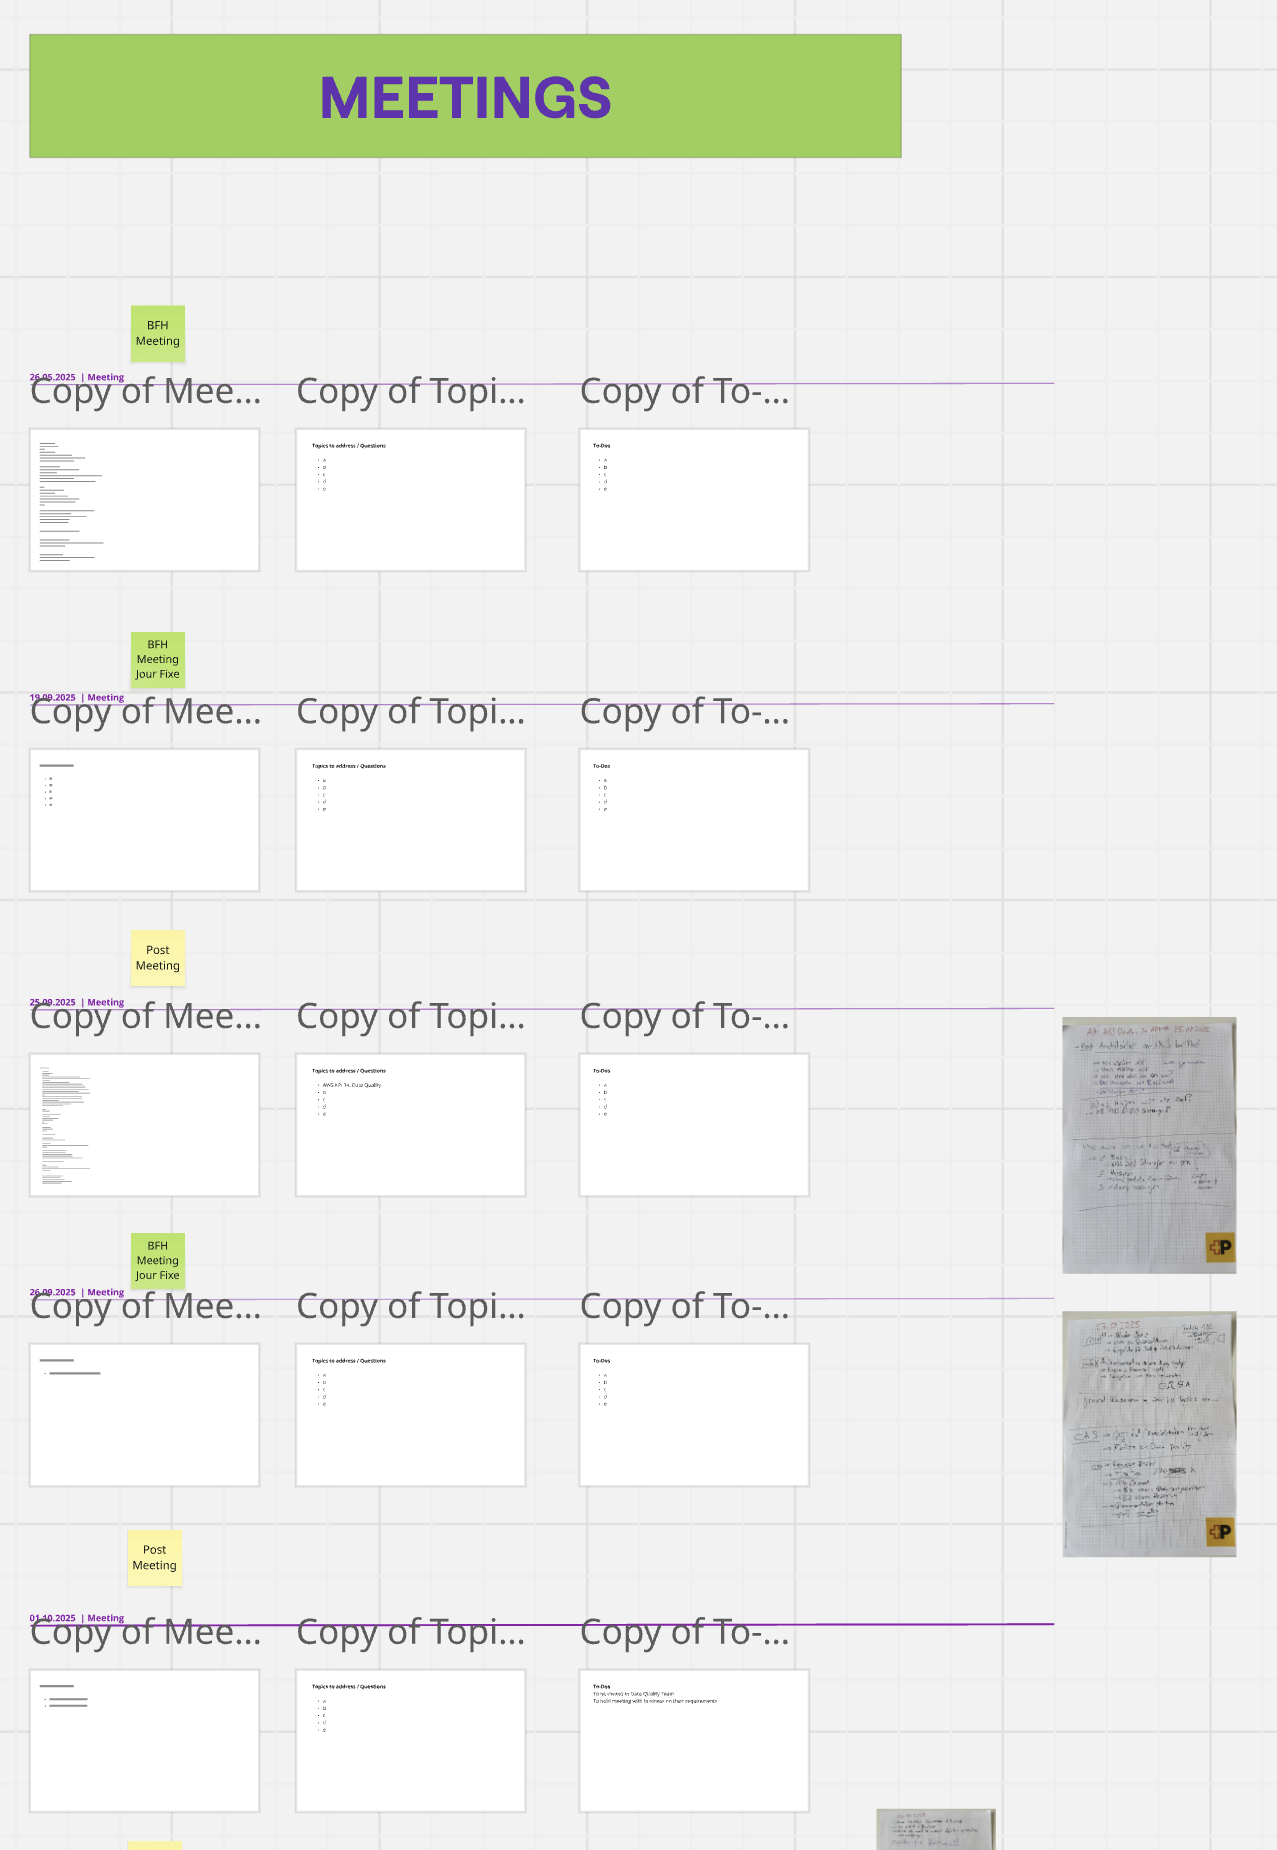
\includegraphics[width=0.8\textwidth]{./content/img/MiroBoard_Meetings.png}
    \caption{Miro board, tracking of meetings: when, who, what}
    \label{fig:miro_board_meetings}
\end{figure}

\subsubsection*{Documentation of the Implementation}
The implementation was first documented in Miro, as the rapid creation of screenshots did not disturb the flow of information gathering. In the following figure, the information-gathering process can be seen, starting from the top left, moving to the right, and then restarting from the left. First, screenshots of the SAC report are shown, followed by navigation towards DSP. Further details on the tools are described in the Implementation chapter.

\begin{figure}[H]
    \centering
    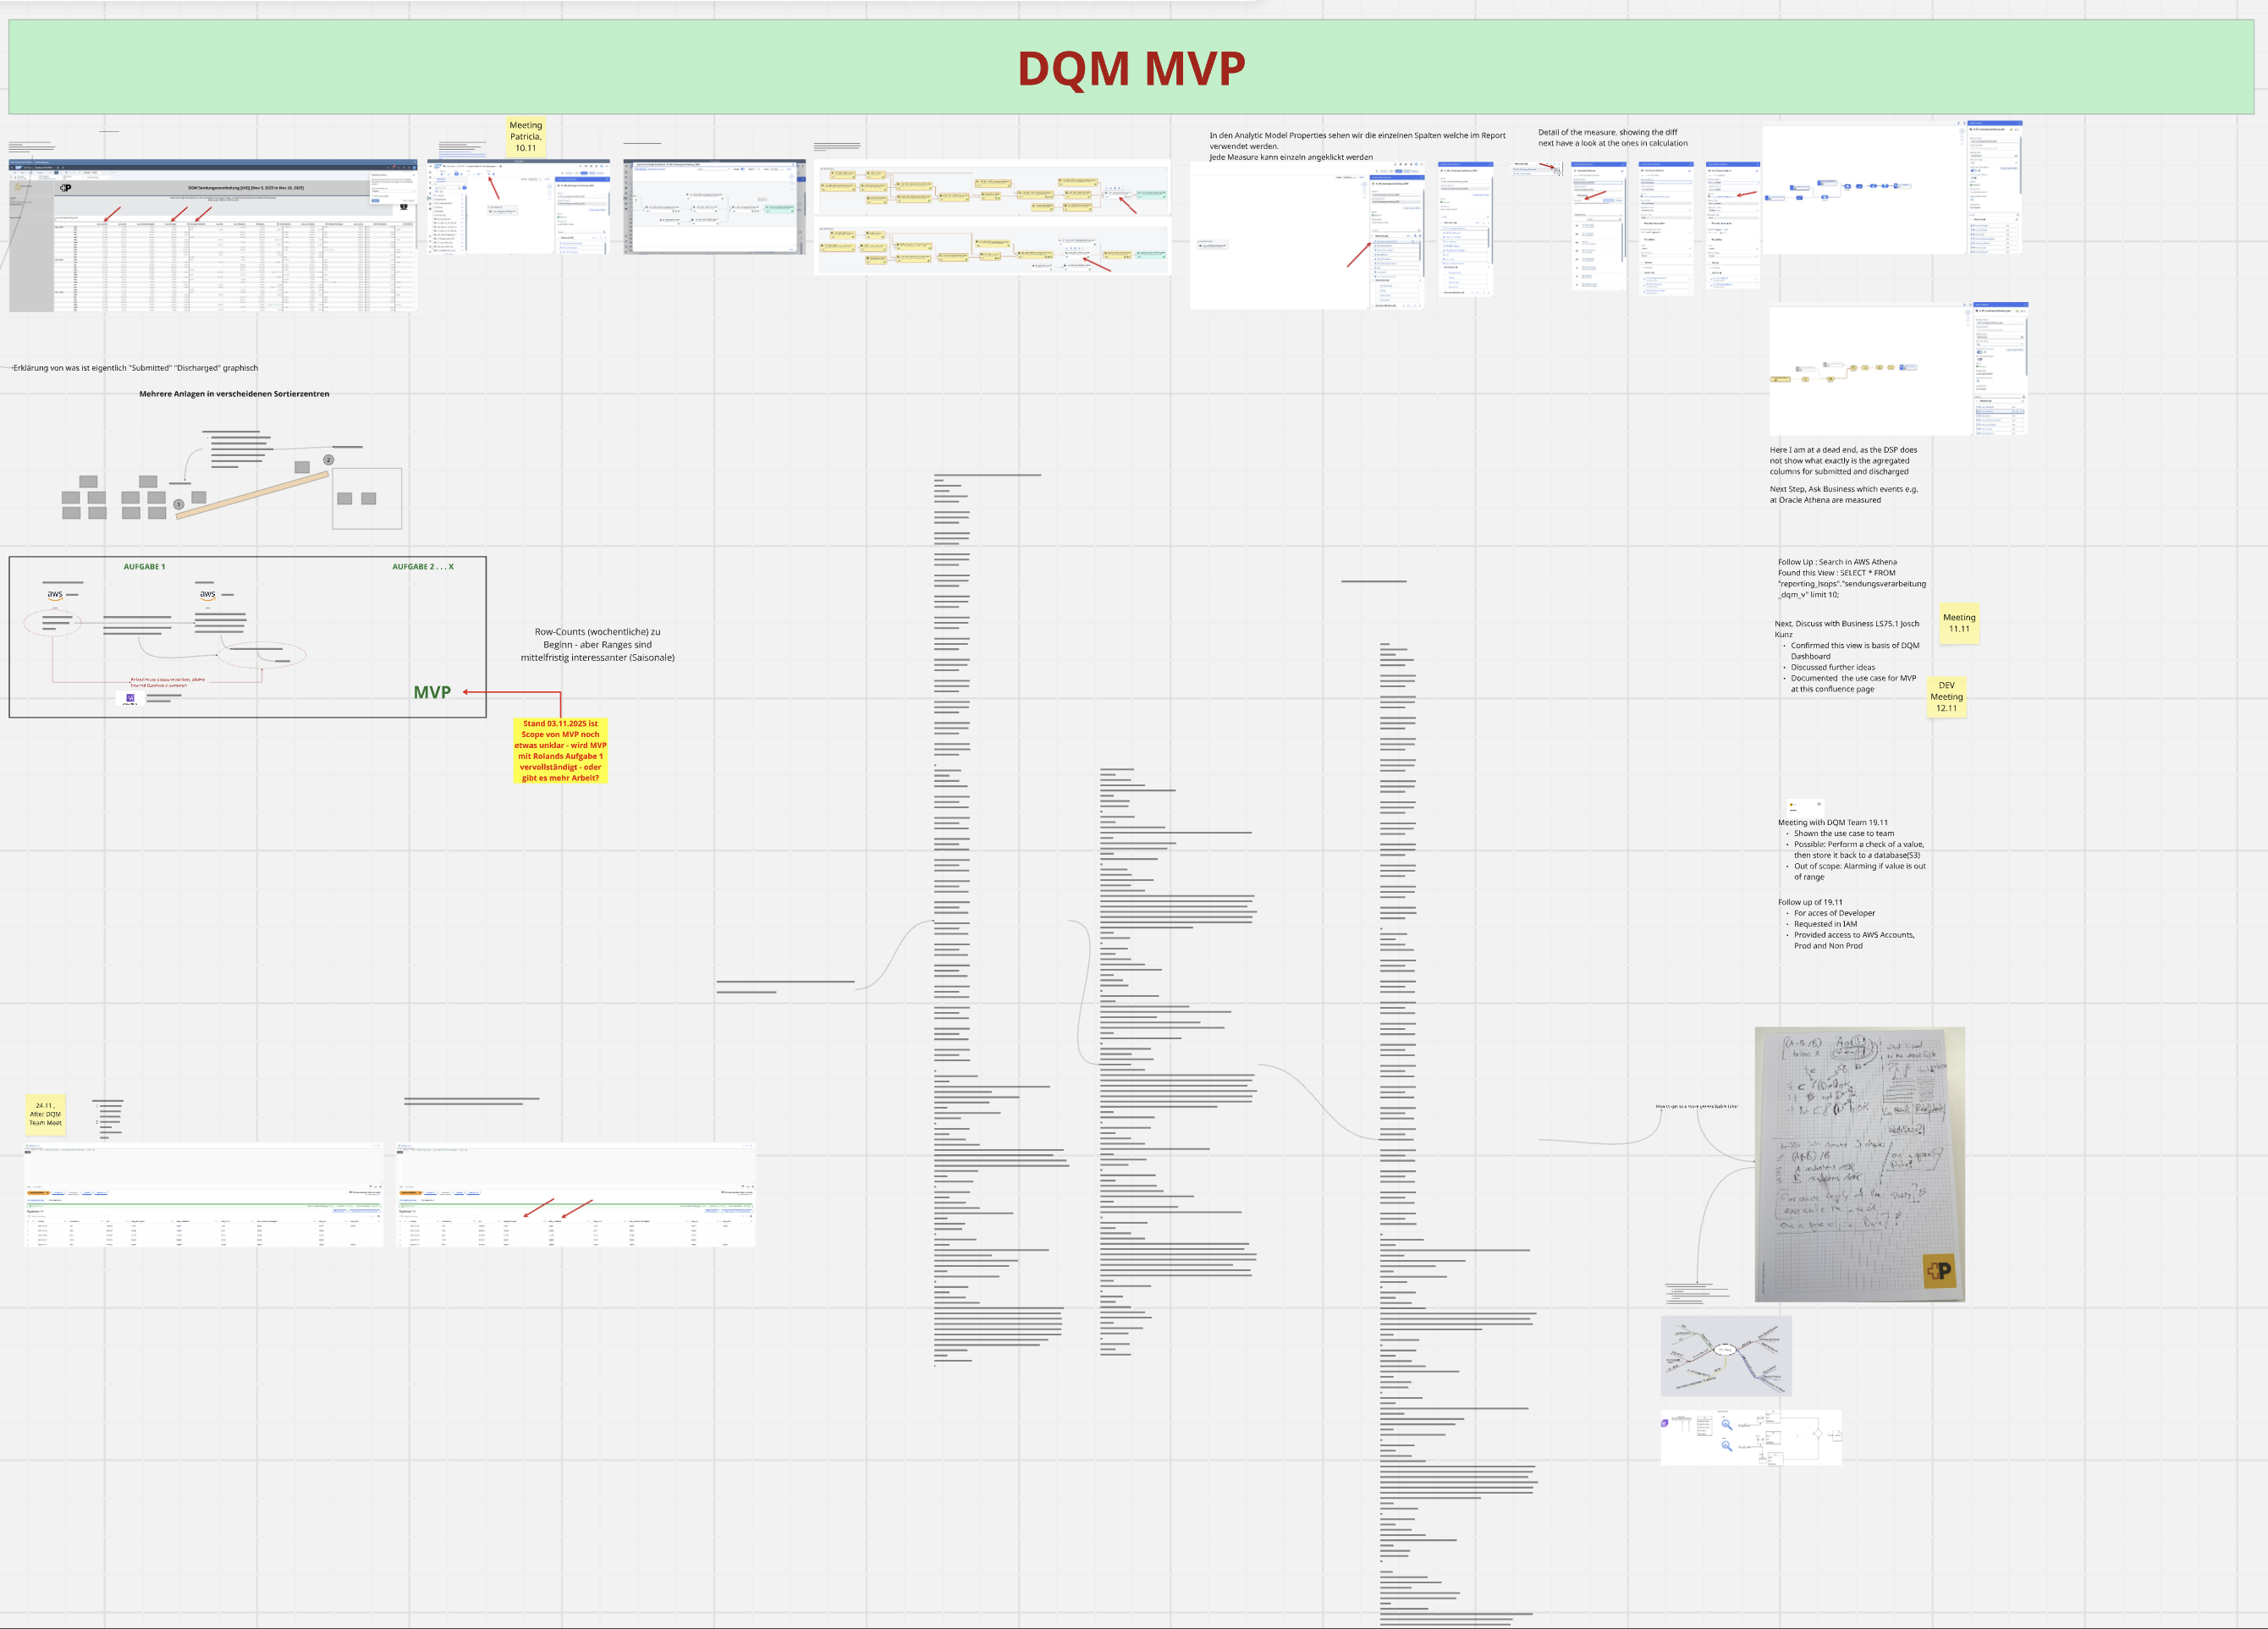
\includegraphics[width=0.8\textwidth]{./content/img/MiroBoard_Implementation.png}
    \caption{Miro board usage for quick documentation during implementation}
    \label{fig:miro_board_implementation}
\end{figure}


\subsection*{Jira and Confluence}

Jira (mainly for issue tracking) and Confluence (mainly for documentation) are both tools provided by Atlassian and are therefore well integrated with each other. The tools are installed on-premises, which limits sharing possibilities outside the Swiss Post network. They are used by the three Swiss Post teams presented in the Teams section. The project team also used Confluence when research results had to be presented as a first use case. While Jira is used for the short-term management of Scrum artefacts, Confluence is used for long-term documentation. An example of such long-term documentation is shown in the following screenshot, illustrating the documentation of a data lineage.

\begin{figure}[H]
    \centering
    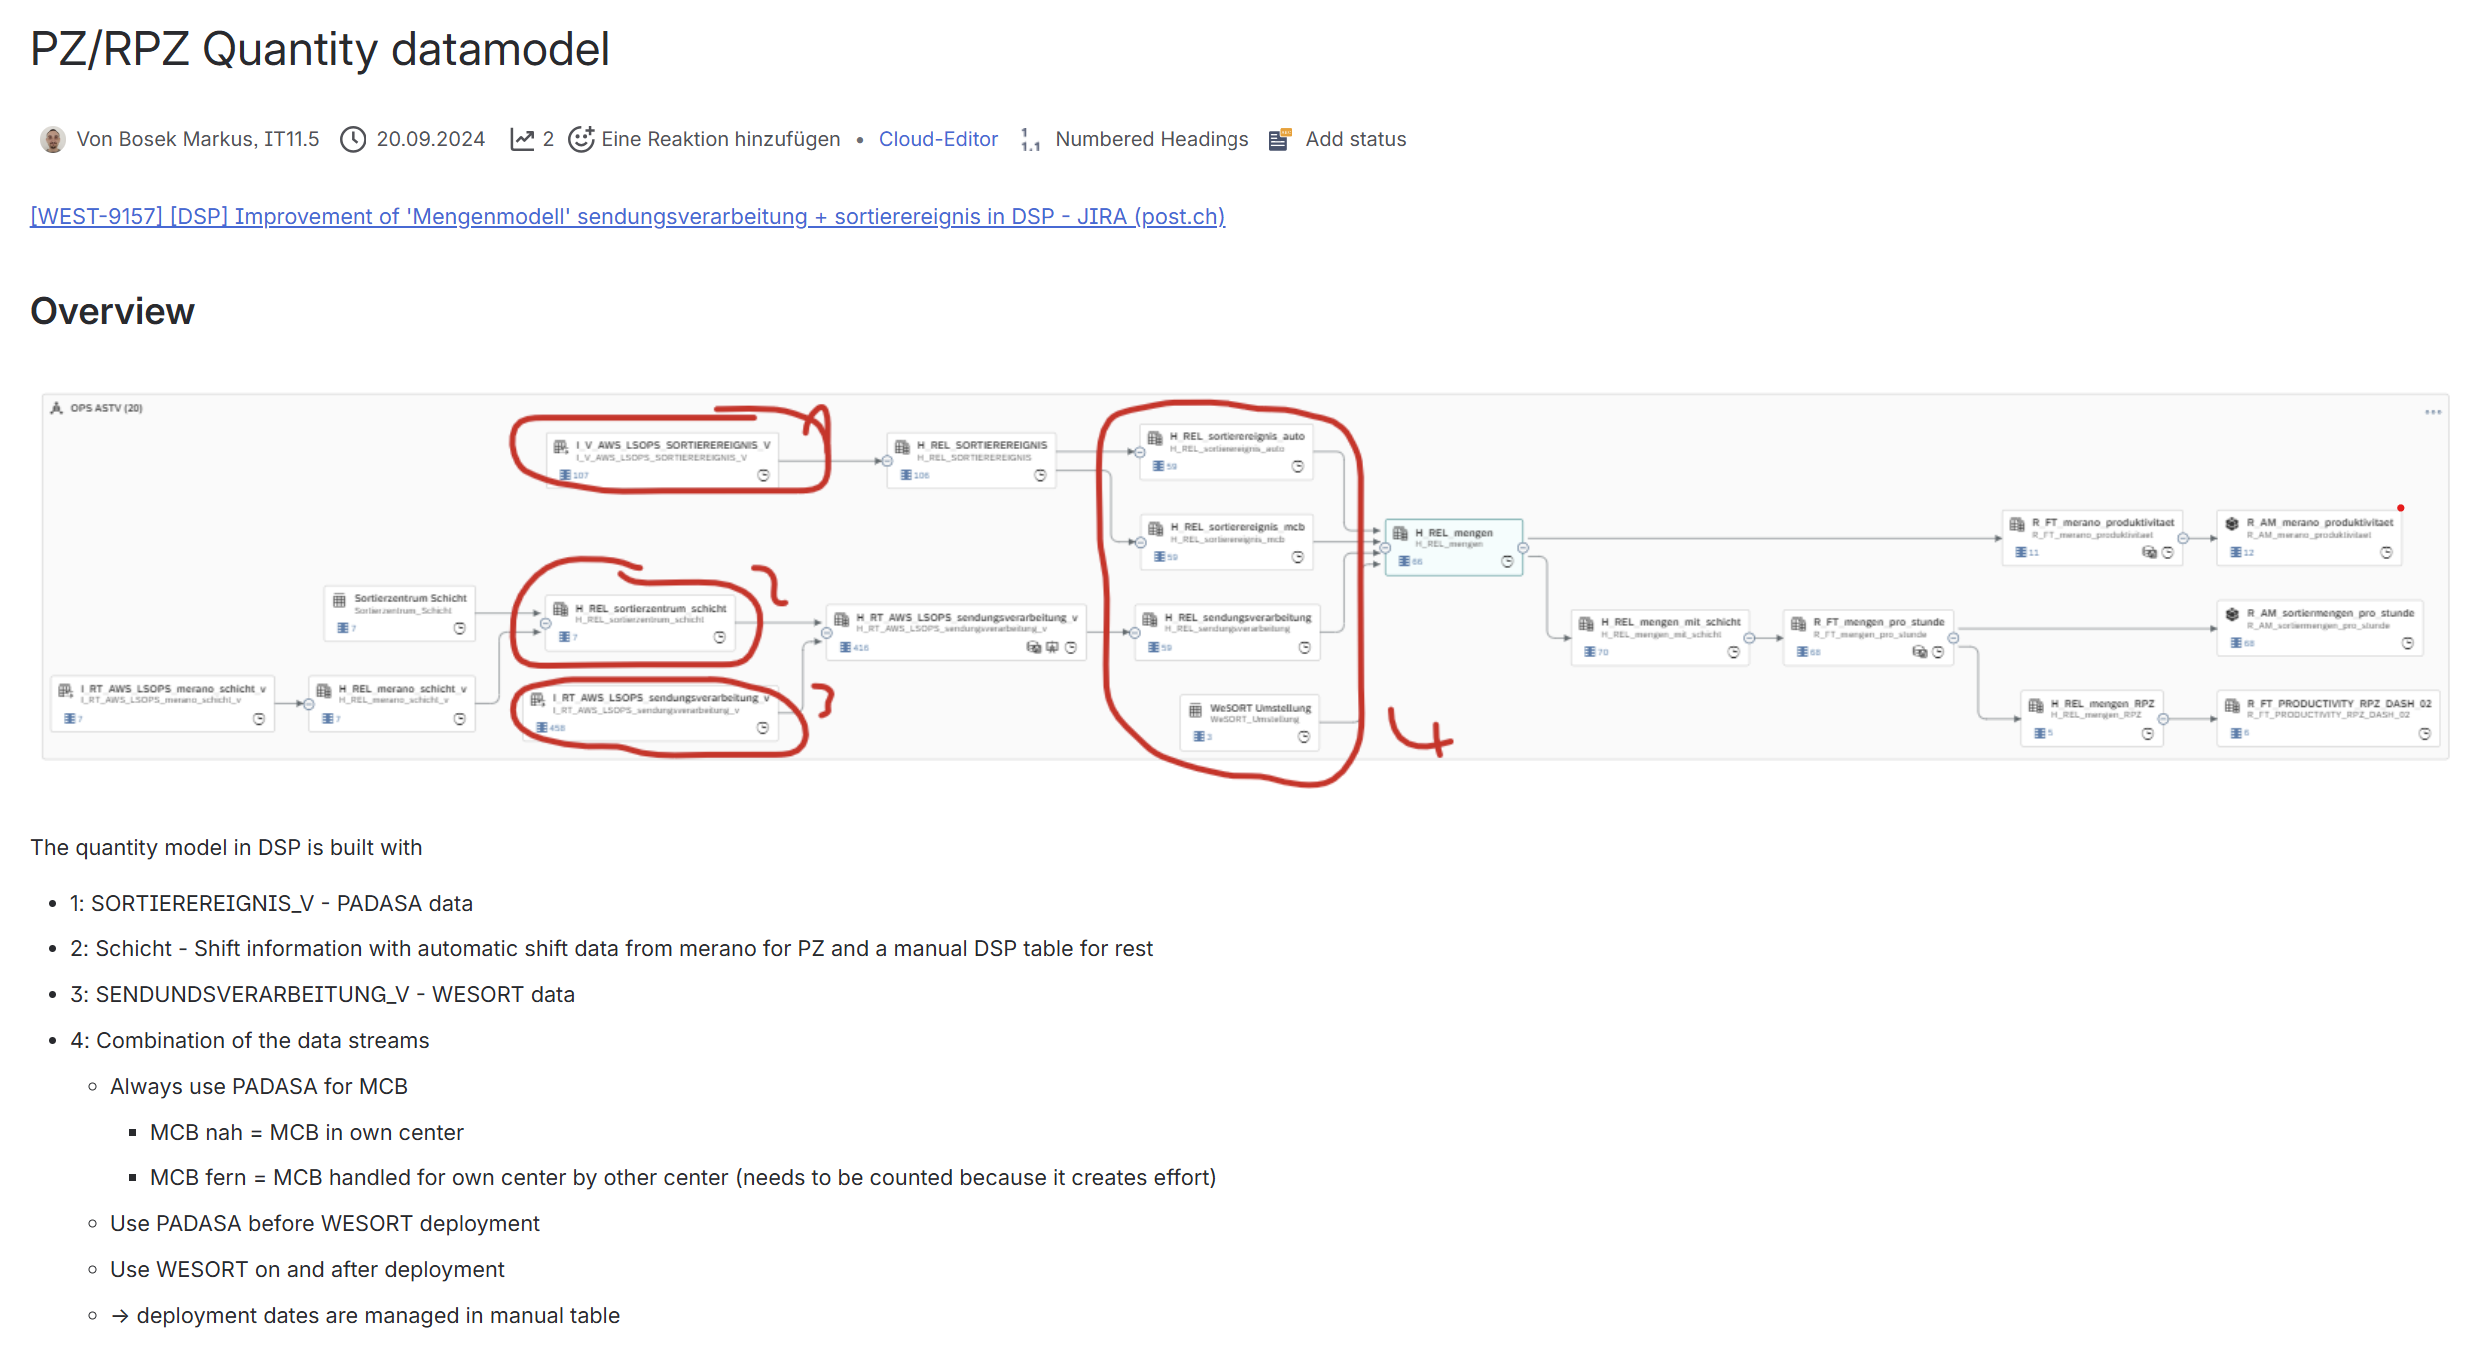
\includegraphics[width=0.95\textwidth]{./content/img/ProjectManagement/Confluence_usage_longtime_documentation.png}
    \caption{Example of project documentation in Confluence used to record architectural decisions and their rationale for future reference}
    \label{fig:confluence_architecture_documentation}
\end{figure}

\subsection*{Microsoft Teams and Microsoft Outlook}
MS Teams and MS Outlook are used by both the academic and Swiss Post teams. They are organisational standards at Swiss Post and are not optional. The same applies to the academic context. Both tools serve to support focused long-term (MS Outlook) and short-term (MS Teams) communication.

\subsection*{Shared chat}
For the academic team, the chat was used for short-term communication. However, a challenge arose due to the involvement of two distinct organisations, BFH and the Swiss Post. In order to keep communication between Swiss Post accounts and BFH accounts in one place, a chat with three users was required. In this context, the cross-organisational capabilities of MS Teams proved useful. After the Swiss Post account was invited to participate in the project team, it was able to communicate directly with BFH accounts. A sample of the communication involving three accounts is shown below.

\begin{figure}[H]
    \centering
    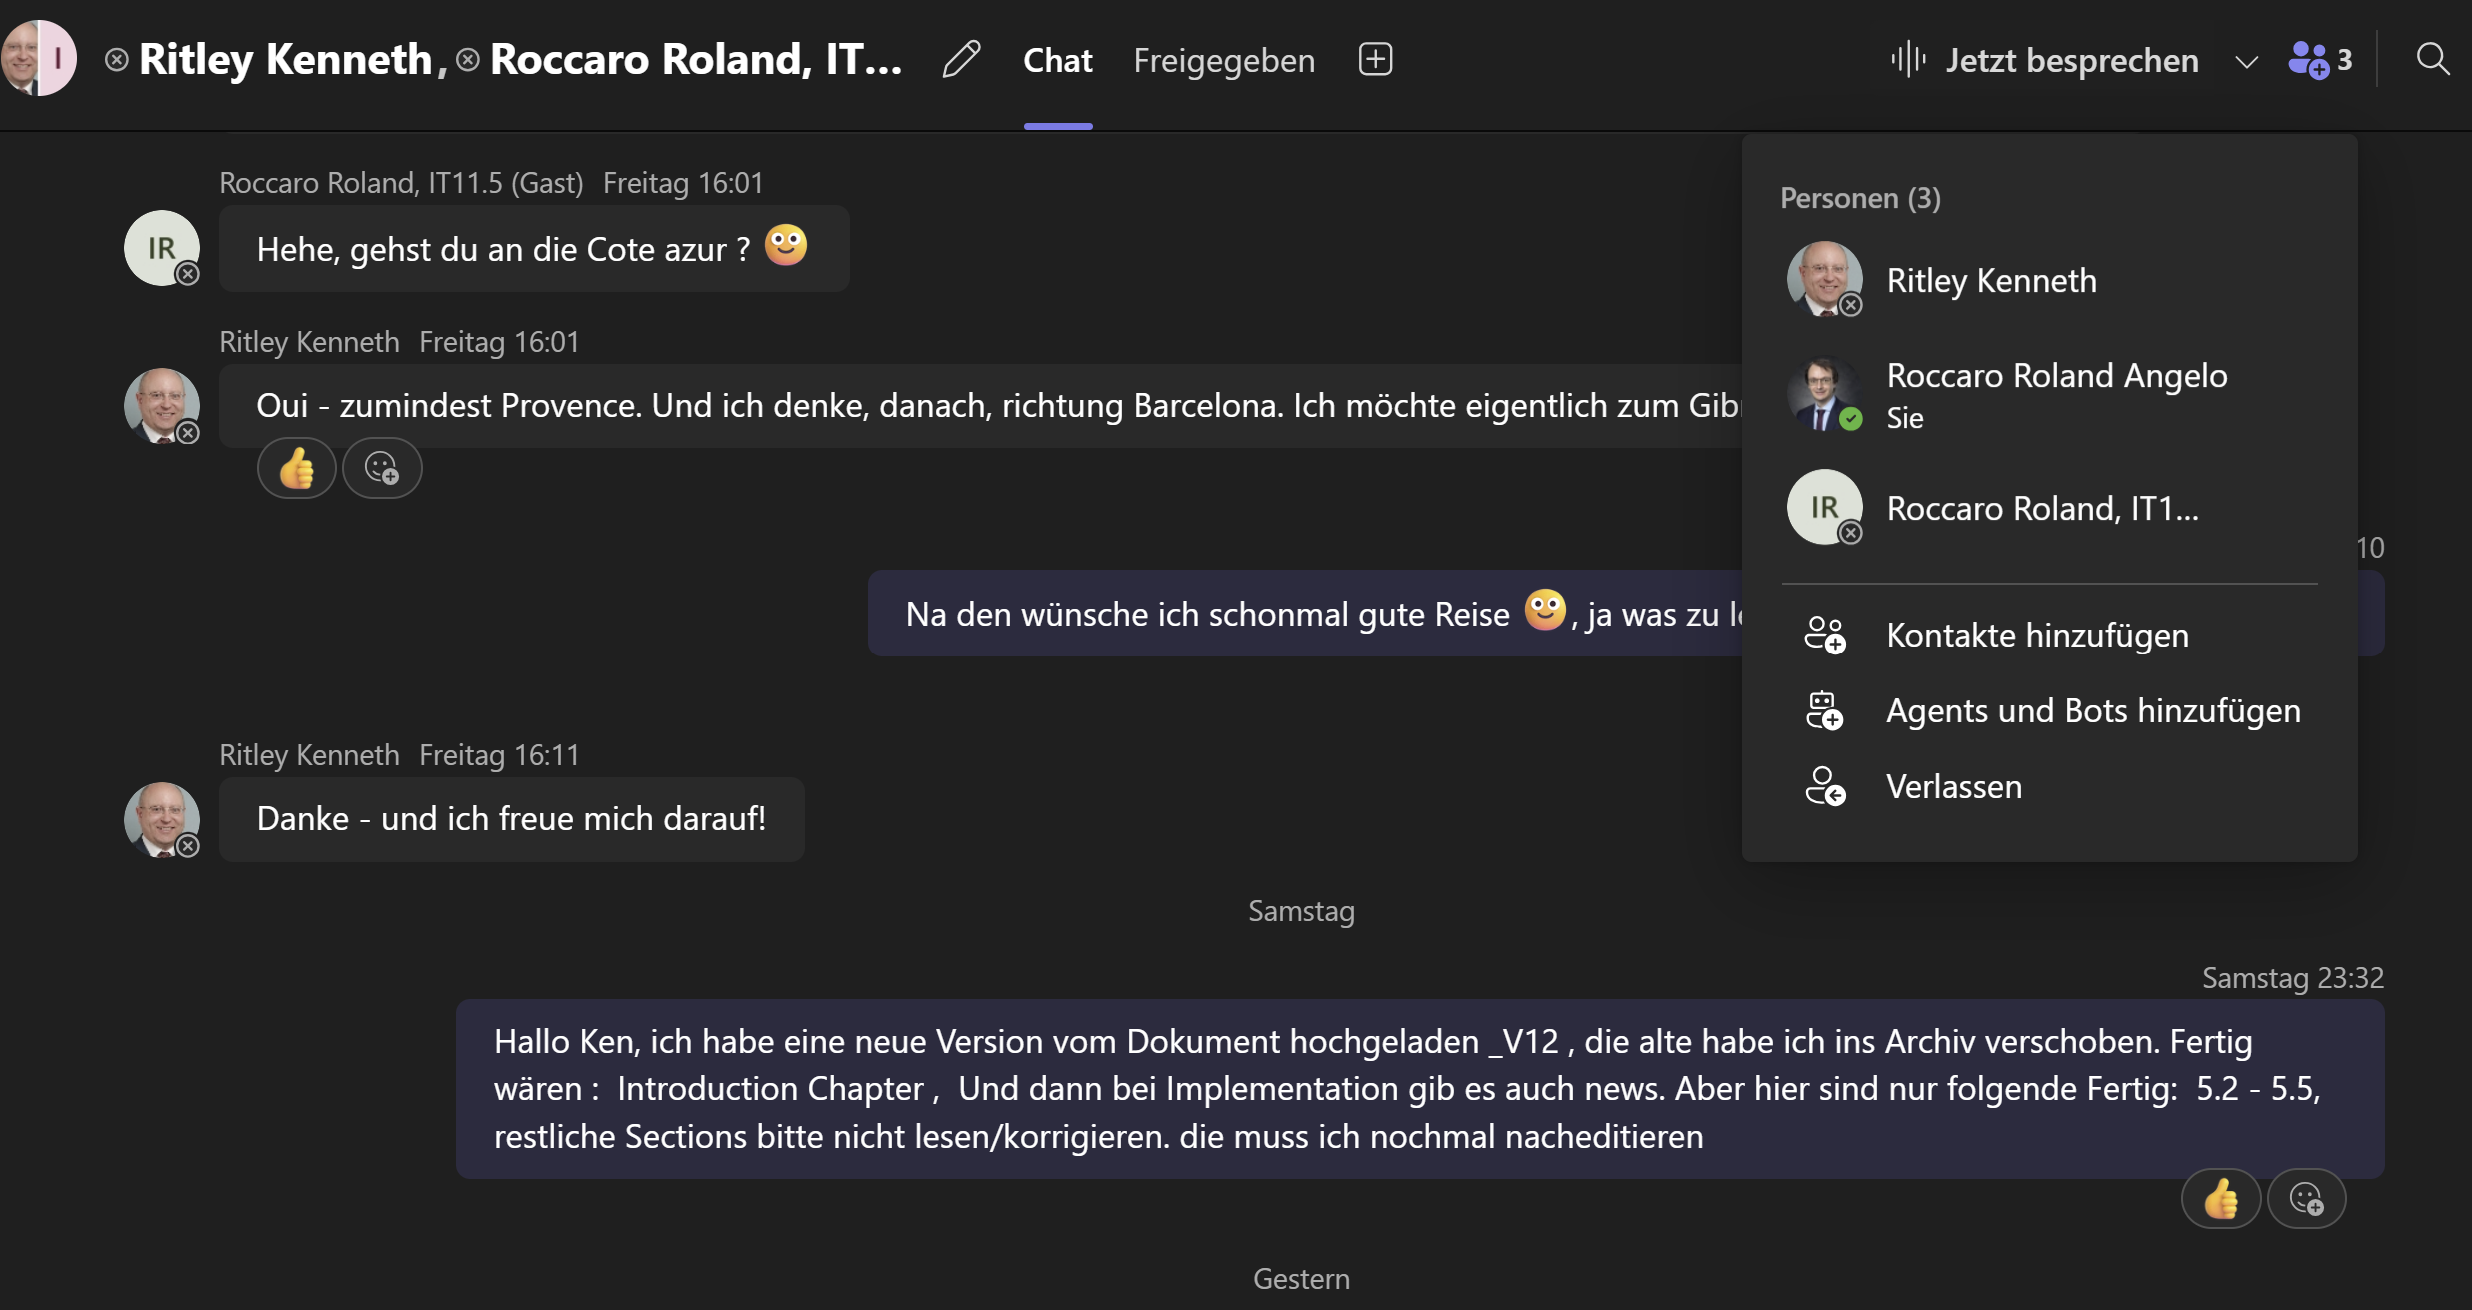
\includegraphics[width=0.8\textwidth]{./content/img/ProjectManagement/ProjMgmt_Teams_Chat.png}
    \caption{Shared chat using Teams}
    \label{fig:teams_shared_chat}
\end{figure}

A second important application of MS Teams is a document management system. This includes source documents, document versions, and related materials. All relevant documents are stored within this structure, which is designed to grow as needed.

\begin{figure}[H]
    \centering
    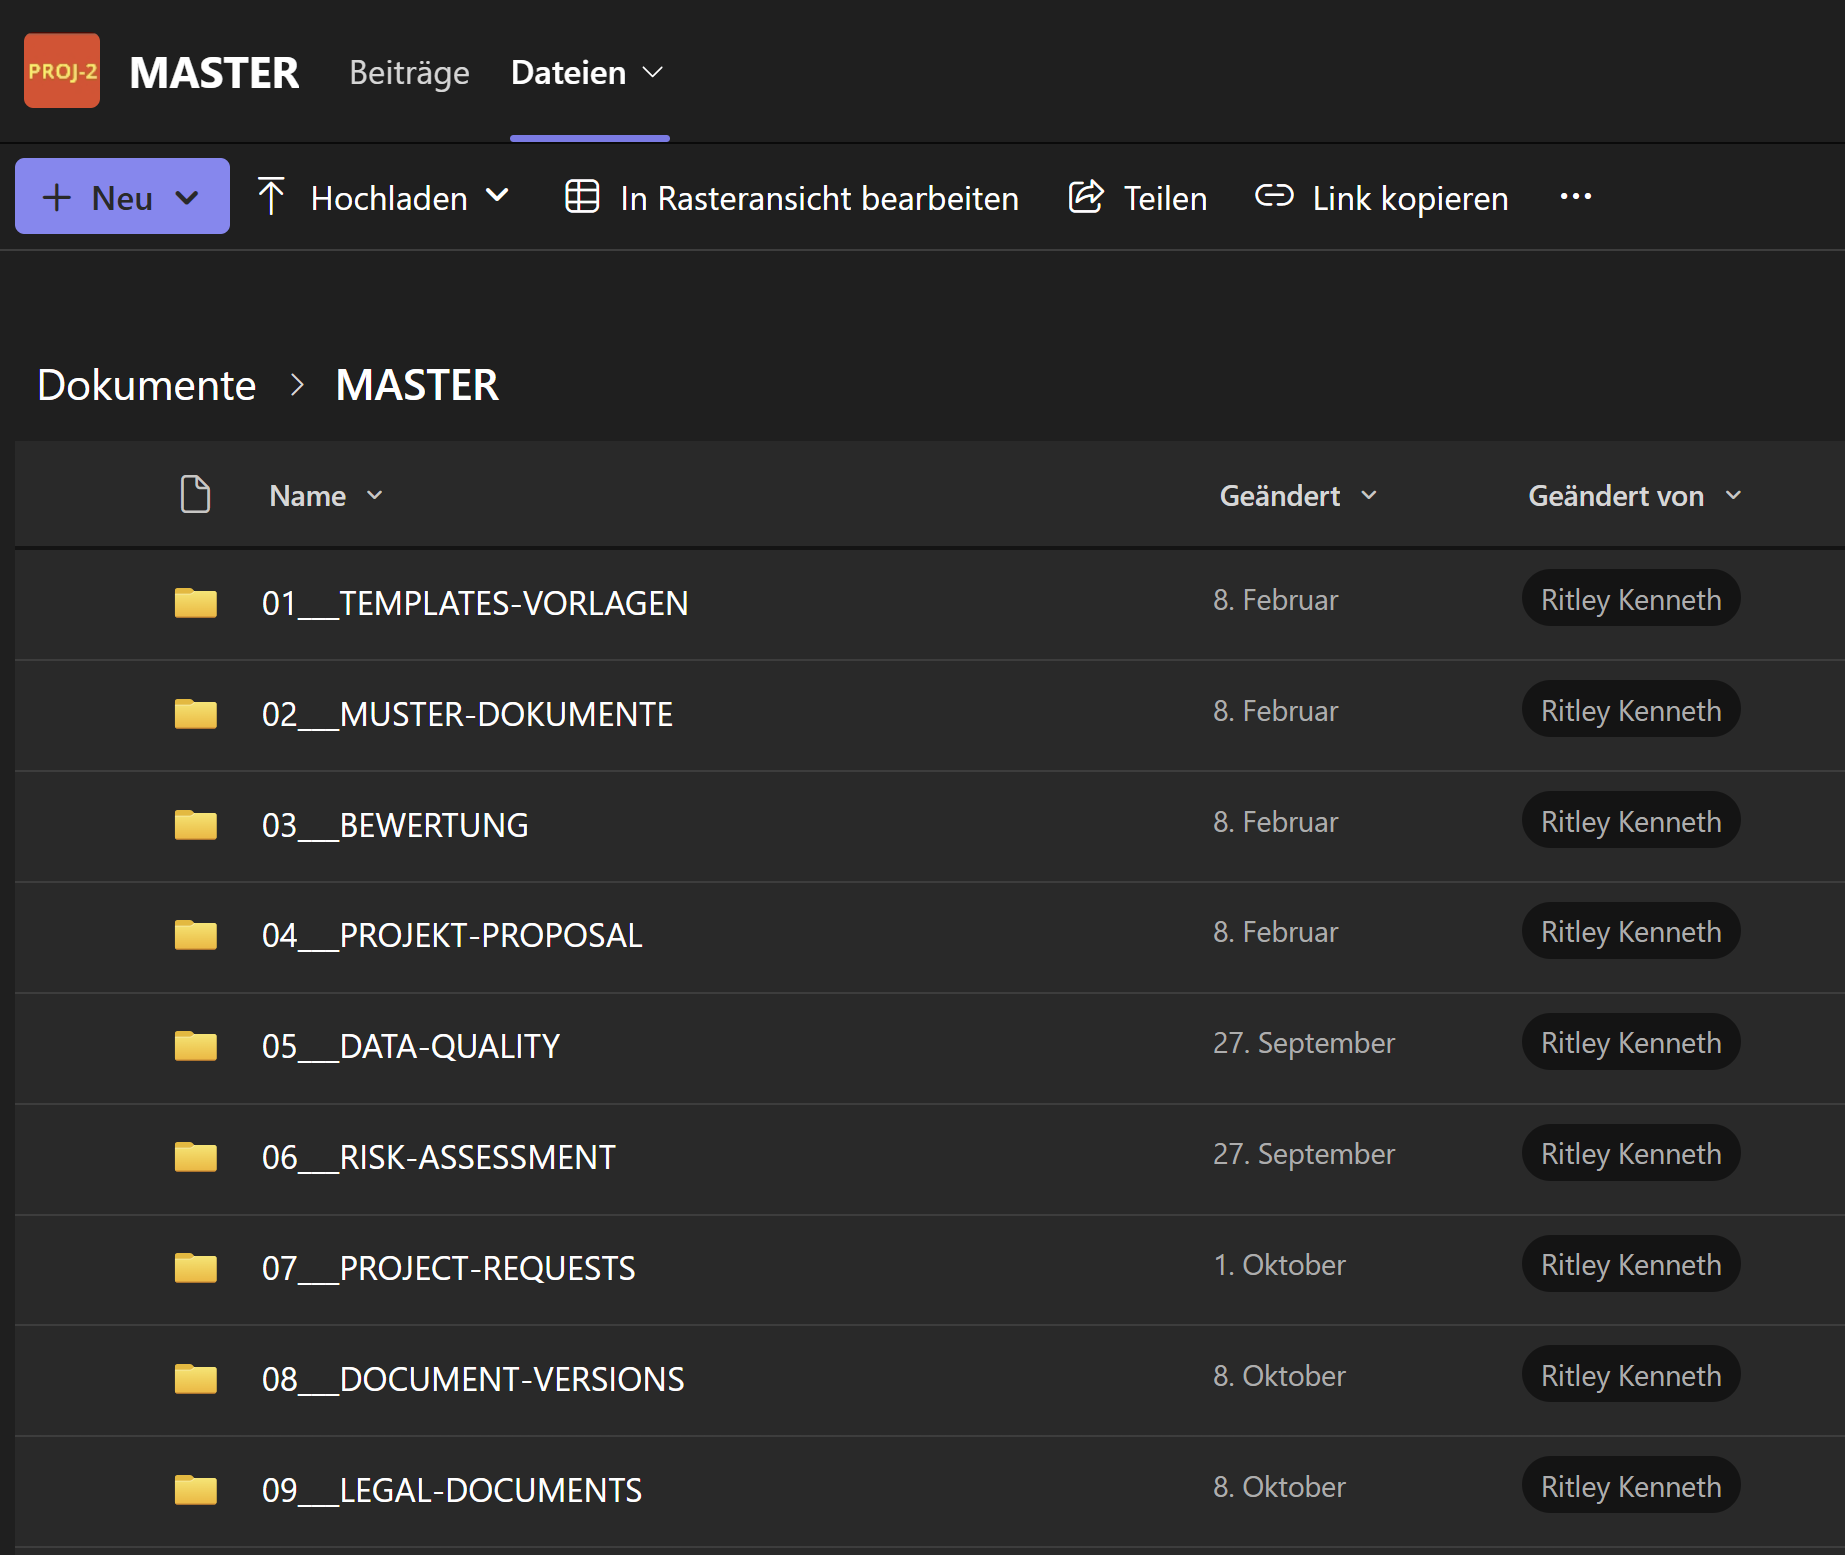
\includegraphics[width=0.8\textwidth]{./content/img/ProjectManagement/ProjMgmt_Teams_Documents.png}
    \caption{Project document store used with Teams}
    \label{fig:teams_document_store}
\end{figure}

\subsection*{LaTeX}
LaTeX was the tool chosen for the main writing process by the academic team. The primary reason for selecting this tool was the consistency of the document structure. It allows changes to be made in a large document without the document becoming unstable. The tool was specifically selected for this higher consistency compared to Word. The fact that the creation of some stylistic elements takes more time than with a \gls{WYSIWYG} editor such as Word was accepted, particularly as design was valued lower than document content. Finally, the consistency of being able to reference text sections within the document and the ability to automatically generate lists of figures and tables were seen as additional benefits. Furthermore, the automatic glossary and citation features using Biber were considered advantages for which the slower writing process without a WYSIWYG editor was accepted. Due to the learning effort involved in using \LaTeX, the following badge was earned during the course of the research.

\begin{figure}[H]
    \centering
    
\includegraphics[width=0.65\textwidth]{./content/img/ProjectManagement/RolandMasterOfLatex.png}
    \caption{Humorous illustration symbolising the extensive use of \LaTeX\ throughout the preparation of this report and the associated learning experience during the project.}
    \label{fig:latex_mastery}
\end{figure}

\subsection*{GitHub}
For maintaining version control of any created artifacts, the public GitHub was used with the private account of the academic team. It was mainly used as a repository. This Git distribution was chosen because it is free to use and already well known to the team, with all required accounts in place, so no additional adoption or learning effort was required before starting. GitHub was not only used to store the document and track its progress, but also to manage all required sources such as tables and images used in the document.

For the writing process, the use of GitHub as a backup mechanism was particularly important. As all sources are stored in GitHub, the project was safeguarded against hardware failures of the working device, which is one risk mitigation measure. Continuously committing and pushing changes made the progress of the writing process traceable and supported the iterative writing approach which was chosen. This proved useful when the document PDF could no longer be generated, as the last version that compiled without errors could be identified. Finally, storing the sources on GitHub allowed access from different devices, which was useful when transferring materials such as screenshots from the work device to the study device.

\subsection*{ChatGPT}
LLMs are now an indispensable part of work. To note how ChatGPT was used in this project, it was given the following prompt:
\begin{quote}
Hi ChatGPT, please look at the other chats I have with you and tell me in which ways you supported me during my academic project over the past months since September 2025. Please create a subsection for my scientific work which I can reference.
\end{quote}

The following subsection was completely AI generated content by ChatGPT, without further editing.
{\itshape
\subsubsection*{ChatGPT}

To document the support provided by ChatGPT, a summary of the assistance received during the academic project was generated directly by the tool itself:
The request asked ChatGPT to review prior interactions and describe the ways in which it supported the academic project over the past months since September 2025. The resulting subsection is intended for inclusion in the scientific work and can be referenced accordingly \cite{chatgpt_ai_assistance_2025}.



The following subsection is entirely AI-generated content produced by ChatGPT, without further editing  \cite{chatgpt_ai_assistance_2025}.

\subsubsection*{Use of AI Assistance in the Research Process}

Since September 2025, the author has used the AI language model \emph{ChatGPT} as a supportive tool during the development of this academic project. The assistance provided did not replace independent scientific work but complemented it in the following ways:

\paragraph{Conceptual Clarification and Structuring}
ChatGPT was used to support the clarification of complex theoretical concepts, the refinement of research questions, and the improvement of the logical structure of arguments. This included exploring alternative formulations, identifying conceptual gaps, and supporting the organization of sections and chapters.

\paragraph{Language and Academic Writing Support}
The tool assisted in improving the clarity, coherence, and academic tone of the manuscript. This included rephrasing passages for precision, adjusting wording to meet scientific standards, and supporting grammatical accuracy and stylistic consistency across the text.

\paragraph{Methodological Reflection}
ChatGPT supported reflective discussions regarding methodological choices, including the articulation of research design, limitations, and the justification of selected approaches. All methodological decisions, interpretations, and final formulations remained the sole responsibility of the author.

\paragraph{Iterative Feedback and Revision}
Throughout the research process, ChatGPT was used as an iterative feedback instrument to review draft sections, explore alternative explanations, and identify areas requiring further refinement or clarification.

\paragraph{Ethical and Responsible Use}
ChatGPT did not generate original empirical data, conduct analyses independently, or make autonomous scientific claims. All AI-generated content was critically evaluated, revised, and integrated by the author in accordance with principles of academic integrity and responsible research practice.
}
\section{Timetracking}
As part of the need for transparency and the ability to review the efforts committed to this project, time tracking was performed from the start to the end of this documentation. The tracked time was recorded in two separate ways. Work efforts carried out within Swiss Post were captured directly from the Swiss Post \gls{MIAR} system, noting only the time spent per day without further details on the specific tasks performed. This information was saved in an Excel file and marked as work effort.

Second, academic efforts committed to the project outside the Swiss Post context were recorded directly in an Excel file. For each work block, a separate entry was created. A block represents continuous work on project-related tasks, including short breaks; however, longer breaks, such as lunch, resulted in a new block being created. Excel was used because the Office suite was already in use for other purposes, and the information did not justify storage in a more complex database such as MariaDB. The tracked time is not intended for billing or performance measurement, nor is it used to assess milestone performance.


\section{Risk management}
\label{ProjMgmtRisk}
In this section, the approach taken to risk management is described. Risk management is essential to the success of any project, as it enables planning for and potentially preventing dangers that may occur during its course. When such risks are not handled, they can endanger the progress of the project. The risk management process consists of several steps \cite{RiskmgmtWikipedia}. First, the risks are identified and classified as to their nature. Next, they are weighted according to how they might impact this project; this includes a consideration of the probability that the risks may arise, and the level of damage that may occur. After this, the specific handling of each risk is defined; these are the concrete measures that are taken to lower how the risk may impact the project. Finally, ongoing monitoring and review of the risks is carried out on a regular basis throughout the project.

\subsection*{Risk identification and classification}

The identification of risks has been carried out for this project, following an extensive brainstorming approach. Each risk has been grouped into a category (e.g. goal, time and organization, etc.), and each risk has been classified according to the likelihood of is occurance and severity it would cause to the project. Both criteria are evaluated based on the project team’s \gls{riskappetite} and ranked according to the following definitions.

\begin{itemize}
    \item \textbf{Likelihood:} What is the expected likelihood of a risk coming into effect
    \begin{itemize}
        \item \textbf{1} Rare
        \item \textbf{2} Unlikely
        \item \textbf{3} Possible
        \item \textbf{4} Likely
        \item \textbf{5} Almost Certain
    \end{itemize}

    \item \textbf{Severity:} How severe are the consequences of the risk coming into effect
    \begin{itemize}
        \item \textbf{1} Insignificant
        \item \textbf{2} Minor
        \item \textbf{3} Moderate
        \item \textbf{4} Major
        \item \textbf{5} Severe
    \end{itemize}
\end{itemize}

The identified  risks, along with their likelihood and severity, are listed in Table \ref{tab:risks}.

\begin{longtable}{@{} C{1.1cm} L{3.2cm} L{8.1cm} C{1.6cm} C{1.6cm} @{}}
\caption{Project Risk Overview}\label{tab:risks}\\


\toprule
\textbf{No.} & \textbf{Group} & \textbf{Risk} & \textbf{Likelihood} & \textbf{Severity} \\
\midrule
\endfirsthead

\toprule
\textbf{No.} & \textbf{Group} & \textbf{Risk} & \textbf{Likelihood} & \textbf{Severity} \\
\midrule
\endhead

\midrule
\multicolumn{5}{r}{\small Continued on next page} \\
\endfoot

\bottomrule
\endlastfoot

1  & Goal & Unclear question & 2 & 2 \\
2  & Goal & Unclear goals & 2 & 3 \\
3  & Time and Organisation & Insufficient expertise & 4 & 2 \\
4  & Time and Organisation & Underestimated time/effort & 4 & 3 \\
5  & Time and Organisation & Other study projects & 3 & 3 \\
6  & Time and Organisation & Work projects & 4 & 3 \\
7  & Time and Organisation & Procrastination & 3 & 2 \\
8  & Human Resources & Unavailability of main project staff (e.g., due to illness) & 4 & 4 \\
9  & Human Resources & Unavailability of advisor (e.g., due to illness, accident, etc.) & 3 & 4 \\
10 & Tech and Infrastructure & Software Version/Library/Dependency & 4 & 3 \\
11 & Tech and Infrastructure & Hardware is damaged & 2 & 5 \\
12 & Data and Research & Data related & 4 & 3 \\
13 & Data and Research & Not reproducible work & 2 & 5 \\
14 & Ethical and Legal & Plagiarism or wrong citation & 2 & 5 \\
15 & Ethical and Legal & Copyright & 1 & 5 \\
16 & Communication and Cooperation & Bad communication with stakeholder or advisor & 2 & 4 \\
17 & Communication and Cooperation & Insufficient exchange with external partners & 1 & 5 \\
18 & Force Majeure & Unforeseen family crisis & 2 & 5 \\
19 & Force Majeure & General force majeure & 1 & 5 \\
\end{longtable}


\subsection*{Risk heat map}
After carrying out the initial identification and classification, it is not always easy to determine which risks require the most attention. To support this task, a Risk Heat Map is used, in which each risk is plotted in a two-dimensional matrix according to its likelihood and severity. This visualisation highlights the risks that pose the greatest threat to the project and should be considered for priority treatment. The colours in the Risk Heat Map \ref{tab:risks_sev_likely} correspond to these descriptions.


\begin{itemize}
    \item \textbf{Green} Low
    \item \textbf{Yellow} Medium
    \item \textbf{Orange} High
    \item \textbf{Red} Very High
\end{itemize}


\begin{table}[h]
\centering
\setlength{\tabcolsep}{3pt}
\renewcommand{\arraystretch}{1.6}
\label{tab:risks_sev_likely}
% 7 columns total: [1] merged "Severity" column + [2] row labels + [5] severity levels
\begin{tabular}{|C{1.3cm}|C{2.8cm}|*{5}{C{2.6cm}|}}

% --- Top black title row: span first two columns for title, last five for "Severity" header label ---

\hline
\rowcolor{black}
\multicolumn{2}{|c|}{\color{white}\bfseries Risk Matrix} &
\multicolumn{5}{c|}{\color{white}\bfseries Severity} \\
\hline

% merged first column (6 rows high)

\multirow{6}{*}{\cellcolor{white}{\color{black}\bfseries \rotatebox{90}{Severity}}}
  & \cellcolor{riskgrey}{}  % empty label cell
  & \cellcolor{riskgrey}\bfseries 1: Insignificant
  & \cellcolor{riskgrey}\bfseries 2: Minor
  & \cellcolor{riskgrey}\bfseries 3: Moderate
  & \cellcolor{riskgrey}\bfseries 4: Major
  & \cellcolor{riskgrey}\bfseries 5: Severe \\
\hline

% ---- Row 1 ----
& \cellcolor{riskgrey}\bfseries 5: Almost Certain
& \cellcolor{riskyellow}{\bfseries 15\; 17\; 19\;}
& \cellcolor{riskorange}{\bfseries 11\; 14\;}
& \cellcolor{riskred}{}
& \cellcolor{riskred}{}
& \cellcolor{riskred}{} \\
\hline

% ---- Row 2 ----
& \cellcolor{riskgrey}\bfseries 4: Likely
& \cellcolor{riskyellow}{\bfseries}
& \cellcolor{riskorange}{\bfseries 16}
& \cellcolor{riskorange}{\bfseries 9}
& \cellcolor{riskred}{\bfseries 8}
& \cellcolor{riskred}{} \\
\hline

% ---- Row 3 ----
& \cellcolor{riskgrey}\bfseries 3: Possible
& \cellcolor{riskgreen}{} 
& \cellcolor{riskyellow}{} 
& \cellcolor{riskorange}{\bfseries 5}
& \cellcolor{riskorange}{\bfseries 4\; 6\; 10\; 12\;}
& \cellcolor{riskred}{} \\
\hline

% ---- Row 4 ----
& \cellcolor{riskgrey}\bfseries 2: Unlikely
& \cellcolor{riskgreen}{}
& \cellcolor{riskgreen}{\bfseries 1}
& \cellcolor{riskyellow}{\bfseries 2\; 7}
& \cellcolor{riskyellow}{\bfseries 3}
& \cellcolor{riskorange}{} \\
\hline

% ---- Row 5 ----
& \cellcolor{riskgrey}\bfseries 1: Rare
& \cellcolor{riskgreen}{}
& \cellcolor{riskgreen}{}
& \cellcolor{riskgreen}{}
& \cellcolor{riskgreen}{}
& \cellcolor{riskyellow}{} \\
\hline

\end{tabular}



\caption{Risk Matrix (Likelihood $\times$ Severity)}
\end{table}

As can be seen in the Risk Heat Map, one risk is classified as red and therefore requires special attention, namely, the unavailability of the main project staff. How this risk, as well as the others, is addressed will be described in the following section.

\subsection*{Risk strategies and mitigation strategies}

Risk strategies are the high level approaches to dealing with the risks, and the risk mitigations are the concrete plans developed to manage identified risks. In the following table, an overview of the individual risks is provided, including their selected treatment and a brief justification. BNaturally, it is neither practical nor feasible to completely eliminate every risk; therefore, based on likelihood and severity, as well as the team’s \gls{riskappetite}, each risk was assigned one of the following strategies:

\begin{itemize}
\item \textbf{Accept} – the risk and its potential impact are acknowledged, but no measures are taken
\item \textbf{Reduce} – the risk is mitigated by applying additional measures to lower its impact or probability
\item \textbf{Transfer} – the responsibility for handling the risk is assigned to another party
\item \textbf{Avoid} – the project is adapted in a way that prevents the risk from materialising
\end{itemize}

\begin{longtable}{@{} C{1.2cm} L{2.5cm} L{4.5cm} L{2.5cm} L{5cm} @{}}
\caption{Risk Strategy and Treatment Plan}\label{tab:risk_treatment}\\

\toprule
\textbf{No.} & \textbf{Risk} & \textbf{Risk Description} & \textbf{Treatment} & \textbf{Treatment Description} \\
\midrule
\endfirsthead

\toprule
\textbf{No.} & \textbf{Risk} & \textbf{Risk Description} & \textbf{Treatment} & \textbf{Treatment Description} \\
\midrule
\endhead

\midrule
\multicolumn{5}{r}{\small Continued on next page} \\
\endfoot

\bottomrule
\endlastfoot

1  & Unclear question & The topic description is too vague or contains too many goals & Reduce & Define SMART goals \\
2  & Unclear goals & The goals are not clearly defined or cannot be measured & Reduce & Describe which goals are part of scope \\
3  & Insufficient expertise & Not knowing required tools or programming languages & Accept &  \\
4  & Underestimated time/effort & Some tasks take more time than initially expected & Accept & Document end of tasks in Miro calendar; re-evaluate after project \\
5  & Other study projects & Other classes demand more attention, less time for project & Accept & Use minimum time for projects/classes \\
6  & Work projects & Other projects at work demand urgent attention, less time for project & Reduce & Reduction of risk due to starting early; defining blockers for study work \\
7  & Procrastination & Tasks are pushed back & Reduce & Start early \\
8  & Unavailability of main project staff & One or multiple project staff are not available & Accept & Document in case it happens \\
9  & Unavailability of advisor & The advisor is not available & Transfer & Advisor to define emergency replacement \\
10 & Software Version/Library/Dependency & Mismatch in versions; new library versions break the code & Accept & Run the code multiple times; have test cases (e.g., unit tests) \\
11 & Hardware is damaged & The laptops or other material are damaged and need repairs or replacement & Reduce & Second laptop; code on GitHub/Miro/Teams/Outlook \\
12 & Data related & Bias in data; not enough data & Accept &  \\
13 & Not reproducible work & The work provided cannot be reproduced & Reduce & Document steps; upload versions on GitHub \\
14 & Plagiarism or wrong citation & Unallowed or undeclared usage of sources & Reduce & Use citation; bibliography \\
15 & Copyright & Used literature or materials which are restricted & Accept &  \\
16 & Bad communication with stakeholder or advisor & Advisor or stakeholders are not heard; their inputs are ignored & Reduce & Weekly advisor meetings \\
17 & Insufficient exchange with external partners & External partners do not react, are delayed, or communication towards them is late or poor & Reduce & Stakeholders in Scrum team \\
18 & Unforeseen family crisis & Unexpected crisis in family & Accept & To be documented in Miro calendar in case it happens \\
19 & General force majeure & Events which cannot be influenced are very rare and very disruptive & Accept & To be documented in Miro calendar in case it happens \\
\end{longtable}

\subsection*{Implementation of risk mitigation strategies}
Identifying the key risks is the first step in the overall risk management approach; this is followed by defining measures for each of the risks. In the following table, the implementation of these measures is documented. The measures have been implemented according to the strategies and descriptions outlined above. Table \ref{tab:risk_actions} provides an overview of the actions taken and when they were carried out.


\begin{longtable}{@{}C{1cm}L{3.5cm}L{9cm}C{2.5cm}@{}}
\caption{Risk Strategy and Action Overview}\label{tab:risk_actions}\\

\toprule
\textbf{No.} & \textbf{Risk} & \textbf{Strategy Decision / What} & \textbf{When} \\
\midrule
\endfirsthead

\multicolumn{4}{c}{\bfseries \tablename\ \thetable{} -- continued from previous page} \\
\toprule
\textbf{No.} & \textbf{Risk} & \textbf{Strategy Decision / What} & \textbf{When} \\
\midrule
\endhead

\midrule
\multicolumn{4}{r}{\small Continued on next page} \\
\bottomrule
\endfoot

\bottomrule
\endlastfoot

1  & Unclear question & In the research section SMART goals have been setup & 23.10.2025 \\
2  & Unclear goals & The introduction describes which parts of the initial project description are part of this document &  \\
3  & Insufficient expertise & Accept: Nothing done & 23.10.2025 \\
4  & Underestimated time/effort & Accept: Nothing done & 23.10.2025 \\
5  & Other study projects & Accept: Nothing done & 23.10.2025 \\
6  & Work projects & Added blockers in Work calendar, Work account invited to meeting series (Jour Fixe); study account: set blockers on weekend; researched with ChatGPT for optimal/minimal study plan & 10.10.2025 \\
7  & Procrastination & Work on the project started 25.09.2025 when attending data quality meeting at AWS, being part of AWS Modernisation initiative & 17.10.2025 \\
8  & Unavailability of main project staff (e.g., due to illness) & Contact of partner provided in Teams and added to Miro board & 23.10.2025 \\
9  & Unavailability of advisor (e.g., due to illness, accident, etc.) & Asked for contact, confirmed to be Jürgen Vogel & 23.10.2025 \\
10 & Software Version/Library/Dependency & Accept: Nothing done & 23.10.2025 \\
11 & Hardware is damaged & Second laptop is available at home; the LaTeX document is a GitHub project; documentation is on Miro. Work laptop can also be used for most tasks, but has no LaTeX installed & 23.10.2025 \\
12 & Data related & Accept: Nothing done & 23.10.2025 \\
13 & Not reproducible work & GitHub project for LaTeX document & 10.10.2025 \\
14 & Plagiarism or wrong citation & JabRef used as GUI for bibliography; Biber used for build & 17.10.2025 \\
15 & Copyright & Accept: Nothing done & 10.10.2025 \\
16 & Bad communication with stakeholder or advisor & Jour Fixe setup & 26.09.2025 \\
17 & Insufficient exchange with external partners & Keep exchange channels active when changing team & 26.09.2025 \\
18 & Unforeseen family crisis & Accept: Nothing done & 23.10.2025 \\
19 & General force majeure & Accept: Nothing done & 23.10.2025 \\
\end{longtable}

\subsection*{Ongoing risk monitoring}
A critical step in the risk management process is ongoing monitoring. Monitoring the risks ensures that the defined measures remain valid and that any risks that may materialise are identified. If a new risk is identified or causes a disruption to the project, it will be documented. Additionally, an appropriate measure to handle its impact will be defined. Monitoring of the risks will be performed every second Friday of each month. Detailed information about the risk monitoring process is provided in the appendix \ref{RiskMonitoring}.
These risk check-ins will contain the following information:

\begin{itemize}
\item Number of risk: same as in the tables above
\item Name of risk: same as in the tables above
\item Occurred: did the risk occur (yes or no)?
\item Details: what happened?
\item Cause: brief analysis of why it happened
\item Measures taken: what measures have been taken?
\item Measure date: on what date were measures taken?
\end{itemize}

\subsection*{Risk review at project completion}

Finally, a review of the risks will be held at the end of the project. This will address which risks came into effect and which did not. Additionally, changes to the perception of the risks will be documented. Because this current project is the first part of a three project series(Project 1, Project 2, Master Thesis) any suggestions to improve the following project will to be described.

\chapter{Topic of this research}
This chapter creates the research foundation for the whole project. It first states the problem addressed and derives the research question. Based on this, the project’s SMART goals are defined to provide clear guidance for the following work. The chapter identifies the research gap that motivates all subsequent work. Finally, core definitions related to data quality and data availability are outlined to provide the theoretical basis for the analysis and implementation that follow.



\section{Problem statement}
\label{ResearchProblemState}
The problem, as defined in the motivation \ref{IntroMotivation} is as follows: reporting at \gls{DWHLSOPS} does not have an automatic alerting system. The data quality and availability reporting at DWH LS OPS is in its infancy, both in regards to data quality as well as automation. This shows itself as: When reports are not executed or contain missing values, IT and the business are not automatically alerted. Due to the lack of automation, no data is gathered on the number of errors and outages.

\subsection*{Business view of reporting}
From the business and end user perspective, the effective reporting cannot be assured. Due to the missing automated checks, it cannot be guaranteed that the system contains complete data as expected on a specific day. The system could display only partial data, for example missing several hours, without informing users. As a result, the business needs to invest additional time to assure users that the report provides correct information.

\subsection*{IT view of reporting}
From the IT perspective, the systems cannot be effectively monitored because the knowledge of what should be monitored is missing. Only the business knows which rules define whether a dataset meets expectations. Therefore, it is very difficult for IT to set up data quality checks. The business is expected to document the expected standards or value ranges before automated checks can be implemented. However, IT also lacks expertise in defining and implementing data quality checks. Furthermore, responsibilities for data quality management within IT teams are not clearly defined. The same applies to data quality dimensions and to the question of when data quality checks should be performed.

\subsection*{Business criticality of reporting}
Due to the lack of automation, the business loses confidence in the new reporting. IT cannot react quickly when reports are not available, as the system does not inform them of missing or incomplete data. Since the checks are currently performed only manually, they cannot be scaled. If the business were required to extend the checks to additional \gls{infoblock}s, even more daily time would be needed to perform these checks. Infoblock is a Swiss Post internal term for data products, combining multiple sources of cleaned data into a complete source for reports including business names. The current situation is therefore not sustainable. From a financial perspective, the checks account for approximately 30 to 45 minutes per day, which results in 130.5 to 195.75 hours per year when calculated over 261 working days (365 days minus weekends, excluding public holidays for simplicity). At an estimated cost of 130 CHF per hour, this corresponds to annual costs of approximately 16'965 CHF to 25'447.50 CHF.

\subsection*{Data reliability and lineage}
Due to the lack of automated checks, it is not known how reliable the reports are. The necessary data to determine how often the reporting system fails to provide data, how often it provides incorrect data, and within which time range the data becomes available are currently missing. Moreover, documentation defining when data is considered correct is entirely lacking. As a result, the current situation requires improvement through the application of best practices, scientific research, and systematic documentation. The foundations for data lineage, data governance, and the definition of \gls{DQ} dimensions are not established and must be defined. Research into both the relevant data lineage and the reporting lineage therefore represents a key problem and a central research objective.

\subsection*{Problem generalisation}
When taking a step back from the very specific problem statement, it is observed that the problem is more generally known as missing formalisation. While initial steps towards running data quality checks with the report mentioned in the business criticality section have been initiated, the rules according to which data quality checks are to be executed, for example when data is considered acceptable or not, were not available at the start of this project. This also applies to the methods by which data quality should be measured, which are not defined. Furthermore, within IT it is not defined who is responsible for running these checks. This situation is a common problem occurring in data-driven companies that lack clear definitions of responsibilities for data quality management. Such definitions need to clarify who performs data quality checks, how data quality checks are performed, which dimensions are checked by data quality checks, and which data quality dimensions exist that could be assessed.



\section{Research gap}
\label{ResearchResearchGap}
Given this problem statement, the following questions are to be researched in more detail within the next two chapters. First, a theoretical introduction of the terms is provided; in later chapters, their specific meaning in the context of this project is discussed:

\begin{itemize}
    \item \textbf{Data lineage}: Identification and documentation of relevant applications in the data flow from source to DWH
    \item \textbf{Benefits of automation}: What are the benefits of automated data quality checks
    \item \textbf{Scalability}: What are the benefits of scalability in DQM
    \item \textbf{Separation of concerns}: How can teams benefit from separation of concerns
    \item \textbf{Reusability across use cases}: Why reusability across use cases is a desired feature
    \item \textbf{Reporting pipeline}: Identification and description of relevant reporting pipeline steps
    \item \textbf{Business workload}: Analysis of current data quality reports performed by the business
\end{itemize}

\subsection*{Data lineage}
Data lineage describes the full lifecycle of data. It answers the question of where data is generated, through which steps of storage, processing, augmentation, and associated IT systems it passes, until it arrives at the DWH. In the context of DQM, this serves as a list of steps at which issues can occur \cite{dama_dmbok}.

\subsection*{Benefits of automation}
In DQM, the automation of the process is an important step. Automation in DQM refers to having check tasks executed by automated systems without additional human interaction during execution or preparation. This is opposed to checks that require human interaction, such as manually combining data sources. Automation provides benefits such as consistency of execution, reduced human error, and repeatability of results \cite{iso9001_automation}.

\subsection*{Scalability}
Scalability is the measure of how well a process can be applied to a larger workload. If a process scales linearly with the number of tasks, it does not scale well. A process must either be optimised by reducing the cost per item as the number of processed items increases, or it must allow multiple processes to run in parallel, which may increase costs but keeps the waiting time for each process low. Scalability is essential for DQM because non-scalable checks lead to increased waiting times or disproportionately rising costs \cite{kleppmann_ddia}.

\subsection*{Separation of concerns}
The separation of concerns is the splitting the responsabilities and building separate components who perform different tasks. This is a design pattern especially valid in terms of DQM. Here this is the separation of business definition from execution of checks. But also having data consumption and validation separated. Finally, quality checks most be distinct from reporting logic. This separation will help to build reusable components beeing more generic rather than each check to be designed completely individually \cite{wikipedia_separation_of_concerns}.

\subsection*{Reusability across use cases}
Reusability across use cases is relevant to DQM, as the same checks are applied to multiple different datasets. For example, a check verifying that category A exceeds a defined threshold is conceptually similar to a check ensuring that category B remains below a defined threshold. When such checks can be reused across multiple use cases, less code needs to be written for each individual check. This is particularly useful in DQM, as similar checks are applied across many datasets, such as validations of date formats, email formats, or plausibility checks. This is a general concept in software engineering and therefore also applies to DQM in IT \cite{sommerville_software_engineering}.

\subsection*{Reporting pipeline}
\label{subsec:ResearchReportingPipeline}
The reporting pipeline consists of the steps through which data passes from the DWH until it becomes consumable in a report. These steps are commonly referred to as the storage layer, the query and processing layer, and finally the reporting and consumption layer.
The storage layer is the entry point into the DWH. It describes how data is initially stored, which may include different processing steps to bring the data into a clean structure. This may already be the case depending on the data source, for example when data is retrieved directly from another database. The second step is the query and processing layer, where data is structured to meet the requirements of specific reports. Queries and joins are used to shape the data according to report use cases, and this step may include additional processing, such as calculating aggregates that are required only temporarily for reporting purposes. The third step, the reporting and consumption layer, is where the data provided through the pipeline is made available to users. At this level, the data is displayed without further modification.
Source: \cite{kimball_lifecycle_toolkit}

\subsection*{Business workload}
The business workload refers to the work that the business currently performs on a daily basis. It is most relevant to this project to understand what activities are carried out daily and how these can be replaced using automation. This gap forms the connection to the next steps to be performed in this and subsequent projects. An important aspect of this step is confirmation from the business that the analysed process is correctly documented and accurately reflects their use case.



\section{High level research question}
\label{ResearchResearchQuestion}
What is the next meaningful step to take in order to improve \gls{DA} and \gls{DQ} within the \gls{DWHLSOPS} team at Swiss Post? How can the Business and IT be supported in achieving their objectives? While the solutions should be as simple as possible, they should be based on best practices and verified through scientific research. The research gap is addressed in the solution and implementation chapters. The main goal is to ensure that the conducted research provides tangible benefits to the team and contributes to future improvements. It is particularly important for the team that the research results are presented continuously, so that progress, as well as potential deviations and changes, can be discussed.



\section{Success definition}
\label{ResearchSuccessDefinition}
The success criteria of this project are threefold and are defined based on the research gap as well as the initial project hand in, which describes the business requirements. 

First, the primary business objective is to achieve automation for the existing report. However, the goal of this project is not to replace the report immediately, but rather to establish concrete steps toward automation. 

Second, communication with the business is another important success factor. The results from research and implementation must be presented on a regular basis to the \gls{PO}. 

Third, the documentation of the data lineage and the reporting pipeline is required, as it forms an important theoretical and practical foundation for future projects and further implementation of DQM.



\section{Smart goals}
\label{ResearchSmartGoals}
The Goals of this project are now defined here as “\gls{SmartGoals}”, as shown in the following list. They are all \textbf{S}pecific: the goal is clearly formulated; \textbf{M}easurable: there are measurable criteria defining when the goal is reached; \textbf{A}chievable: they are realistic given the available resources; \textbf{R}elevant: the goal is directly linked to the project’s success; and \textbf{T}ime-bound: there is a defined timeframe for achievement.


\begin{itemize}
\item \textbf{1) Identification of initial data quality metrics}
    
\textbf{WHY:} This helps to ensure that checks focus on business-relevant issues.

By the end of the analysis phase, the initial data quality measures suitable for automated projects in the DWH LS OPS environment are identified and defined. At least three dimensions should be covered, such as completeness and consistency.

Success is measured by the documented metrics, which include a specific metric definition with calculation logic, data scope, and business relevance.



\item \textbf{2) Investigation of IT systems for DQM metrics}

\textbf{WHY:} To identify how to obtain the needed metrics, and to To define what DQM means in measurable terms.To define what DQM means in measurable terms.

By the end of the analysis phase, the IT systems and data stores are investigated, and it is defined where quality metrics can be implemented, stored, and evaluated within the DWH LS OPS environment.

Success is measured by a documented system overview that maps the selected metric to its technical source, storage location, and execution context. This is to be validated with IT stakeholders.

 
\item \textbf{3) Investigation of data lineage for metrics}

\textbf{WHY:} To apply DQM checks to the correct data sources and enable root cause analysis.

By the end of the analysis phase, investigate and document the data lineage from data ingestion to the reporting layer.

Success is measured by a documented lineage description that allows data to be followed through the system and its transformations to be understood, including the validation possibilities available to responsible stakeholders.


\item \textbf{4) Design and testing of an automated DQM algorithm}

\textbf{WHY:} To verify that DQM checks are the appropriate ones and that they can be automated reliably before full implementation.

By the end of the implementation phase, at least one algorithm that automates a selected DQM check based on defined metrics is designed and tested.

Success is measured by a reproducible implementation and successful execution of the automated check based on the defined metrics.

\item \textbf{5) Implementation and validation of an automated DQM check}

\textbf{WHY:} Not only to To demonstrate that the solution works in practice and can reduce manual DQM effort, but to serve as a first-step in a further expansion of DQM automation.

By the end of the implementation phase, the automated DQM check for the selected use case is implemented and validated based on the designed algorithm and its metrics.

Success is measured by successful execution of the check on productive, representative test data, including documented results across multiple runs and stakeholder confirmation that the check reliably identifies DQM issues without manual intervention.


\end{itemize}



\section{What are data quality checks?}
\label{ResearchWhatIsDQ}
People using the same data can often be in disagreement about what \gls{DQ} means for that data \cite{DQwikipedia}. Data quality can be defined as data being of high quality when it correctly represents the real-world construct it refers to, making it fit for decision-making and planning. To establish a common understanding of data quality, official frameworks have been defined \cite{enwikiISO8000}. These frameworks have specific characteristics, as described here.

\subsection*{Rule based}
A data quality check tests data against rules, expectations, or thresholds and thereby attempts to detect issues. If issues are identified, they are not corrected by the data quality check itself but are instead made visible.

\subsection*{Use case driven}
The type of check applied depends on the use case and business context. Data quality checks must be purposeful for the specific use case and are explicitly defined. For example, a threshold may be defined with an exact value, such as the parcel width being a maximum of one meter on automatic sorting machines.

\subsection*{Manual and automated checks}
Data quality can be assessed manually or through automated checks; both approaches are valid. A manual check is performed by skilled staff and requires their full attention during execution. It includes multiple steps, such as gathering data from different sources and performing aggregations. This makes manual checks slow and difficult to scale; however, they are flexible and can be adapted quickly to changes. In contrast, automated checks are performed by systems on a defined schedule without staff intervention. They are therefore repeatable and deliver consistent results. A manual check can be used to verify data quality once; however, when checks need to be repeated regularly, they should be automated.

\subsection*{Dimensions}
Data quality is measured across multiple dimensions such as:
\begin{itemize}
    \item \textbf{Completeness}: When mandatory fields are present, data is considered complete
    \item \textbf{Accuracy}: How closely the data reflects the real world
    \item \textbf{Consistency}: Whether the same data is consistent across systems
    \item \textbf{Timeliness}: Whether the data is available when it is needed or only at a later time
\end{itemize}
This is only a subset of dimensions that can be considered in data quality checks. These dimensions have, however, already been defined at Swiss Post. Therefore, their further definition is not useful and is not part of this project \cite{iso_iec_25012}.

\subsection*{Detection and correction}
In \gls{DQM} detection and correction of errors is strictly different. In this project, the focus is on the detection of data quality issues. The correction of these issues is out of scope of this work.

\subsection*{Checks on data lifecycle}
\label{ResearchDataQChecksOnDataLifecycle}
The placement of data quality checks on the data lineage and reporting pipeline is an important decision in the process. The different stages are data ingestion or generation, storage and staging, processing and transformation, and reporting and consumption. Running data quality checks at the ingestion level provides only limited checking possibilities, such as structural validity and schema compliance. At the storage and staging level, consistency, deduplication, and format correctness can be checked. Moving further to the processing and transformation stage, checks on joins and aggregations can be performed, as well as plausibility checks of derived values. On the reporting layer, cross report consistency can be checked. In general, checks on earlier layers are more limited, while the processing and transformation layer allows the most meaningful and effective checks.



\section{What are data availability checks?}
\label{ResearchWhatIsDA}
A \gls{DA} check verifies that a defined dataset exists, whether it is available on time, and whether it is accessible. Such checks are binary: the dataset is either available or not.

\subsection*{Distinction to data quality checks}
While a data quality check evaluates the correctness of data, a data availability check determines whether the data is available. Data can therefore be available but incorrect, or correct but unavailable. For example, data may be available for a report at 07:00, which is the required availability time, but the delivered data may be incorrect. Conversely, the same report could be available at 07:15 with correct data; however, it would not be available within the defined time frame.

\subsection*{Temporal dependency}
Data availability is always time dependent. Data can be available at the defined time or not. This requires clear definitions of which data must be available and at what time. In order to check temporal availability, the relevant timeframe must be defined. For example, a report may need to be available at 07:00. However, the data used by this report may be expected earlier, for instance at 06:30. Thus, the same data can have different temporal expectations regarding when it can first be expected and when it reaches its deadline. For every temporal check, these deadlines need to be defined.

\subsection*{Availability and accessibility}
Data can be available but not accessible at the same time. The data and the complete report may exist and be correct; however, a user who requires it may not be able to access it. This can occur due to missing or incorrect access rights. Other scenarios are also possible, such as data being generated initially but not transferred at a later step of the data lineage. In such cases, the raw data is available at an earlier stage but not accessible at the final stage. This can be caused by errors in the pipeline as well as by system outages.

\subsection*{Expectation values}
An expectation check compares whether data is available in defined amounts, time windows, or other specified criteria. For example, at 09:00, nine tons of coal are expected to be in stock. This type of check includes both the expected amount and the defined time window.

\subsection*{Business impact}
When data is unavailable at the defined moment, this causes business disruptions. The severity of the disruption is proportional to the importance of the missing data and the duration of the delay.

\subsection*{Checks on data lifecycle}
When implementing \gls{DA} checks, the same question arises as with \gls{DQ}: at which stage it is most efficient to implement them. For data availability checks, the general rule is that earlier is better. If data is not available at the ingestion stage, all subsequent steps depending on it will also fail. When checks are performed on the storage layer after ingestion, the presence of data in the DWH can be verified. If an earlier data availability check was successful, an issue at the transport or DWH level can be identified. When moving further up to the processing and transformation layers and finally to the reporting and consumption layers, the check becomes highly visible, as a report is either present or not. However, this only allows identification of whether users experience an issue, not where it originates. Overall, earlier data availability checks yield better results for IT when identifying errors and correcting them.
\chapter{Solution landscape}
In order to enable the reader to understand the complexity of the Swiss Post \gls{DWHLSOPS}, the data lineage must be presented at a high level. This chapter provides an overview of this lineage while deliberately omitting details that are not relevant to this project. It further explains the scope of this project within the data lineage and describes the reporting lineage with relevant tools. Furthermore, it is important to note that the solution landscape reflects the current state of knowledge and is limited to the project scope. Any additional knowledge acquired during implementation is discussed in the Results and Target Analysis chapters.


\section{The Swiss Post addresses data quality in multiple ways}
\label{SolutionMultipleTeams}
At the start of this project, the objective was to develop a minimal viable product (\gls{MVP}) to replace a manual data quality check performed by the business with a more robust solution, including automation, the delivery of reports, as well as an appropriate notification and alerting. However, after beginning this project, Swiss Post management assigned a new priority to the topic of data quality management (\gls{DQM}) overall; therefore, quite unexpectedly, this project acquired an additional set of key stakeholders, located in different teams as discussed in chapter \ref{sec:AWSmodernisationteam}. 


Fortunately, this project as originally conceived fit very well into the larger \gls{DQM} picture.  Coordination with these teams although not originally envisioned (such as the DQM team described in chapter \ref{sec:DQMteam}) therefore became an important task. This coordination was essential for several reasons: first and most obviously,  the project must avoid reinventing existing solutions or overlapping in an unplanned way with other new initiatives. Second, it must ensure that methods and deliverables of this project conform to any new data architecture standards; for example, data quality dimensions have already been defined and documented by other teams. Finally, it must ensure that ongoing work by other teams is taken into account. 



\section{Rule-Based DQM Initiative}
\label{DQMRuleBasedInitiative}

The current architectural goal pursued by the \gls{DQM} team is shown in the following visualisation. The rule evaluation engine, shown at the top centre, executes defined rules on target data and stores the corresponding rule results in a database. In this context, a rule represents a data quality check for a defined dataset, and many different rules can be defined. These rules may, for example, specify allowed values, such as restricting the gender attribute to the three values \textit{male}, \textit{female}, and \textit{not stated}. Alternatively, they may define expected data types, such as requiring dates to be stored in UTC format, or specify valid value ranges depending on the weekday.

Although the rule evaluation engine was a major topic during the weekly exchanges with the \gls{DQM} team, it was not implemented by the project team. Nevertheless, its development progress was regularly monitored and discussed during these meetings. Furthermore, the \gls{ASTV} team used this tool for its intended purpose. However, this usage was outside the scope of this project.


\begin{figure}[H]
    \centering
    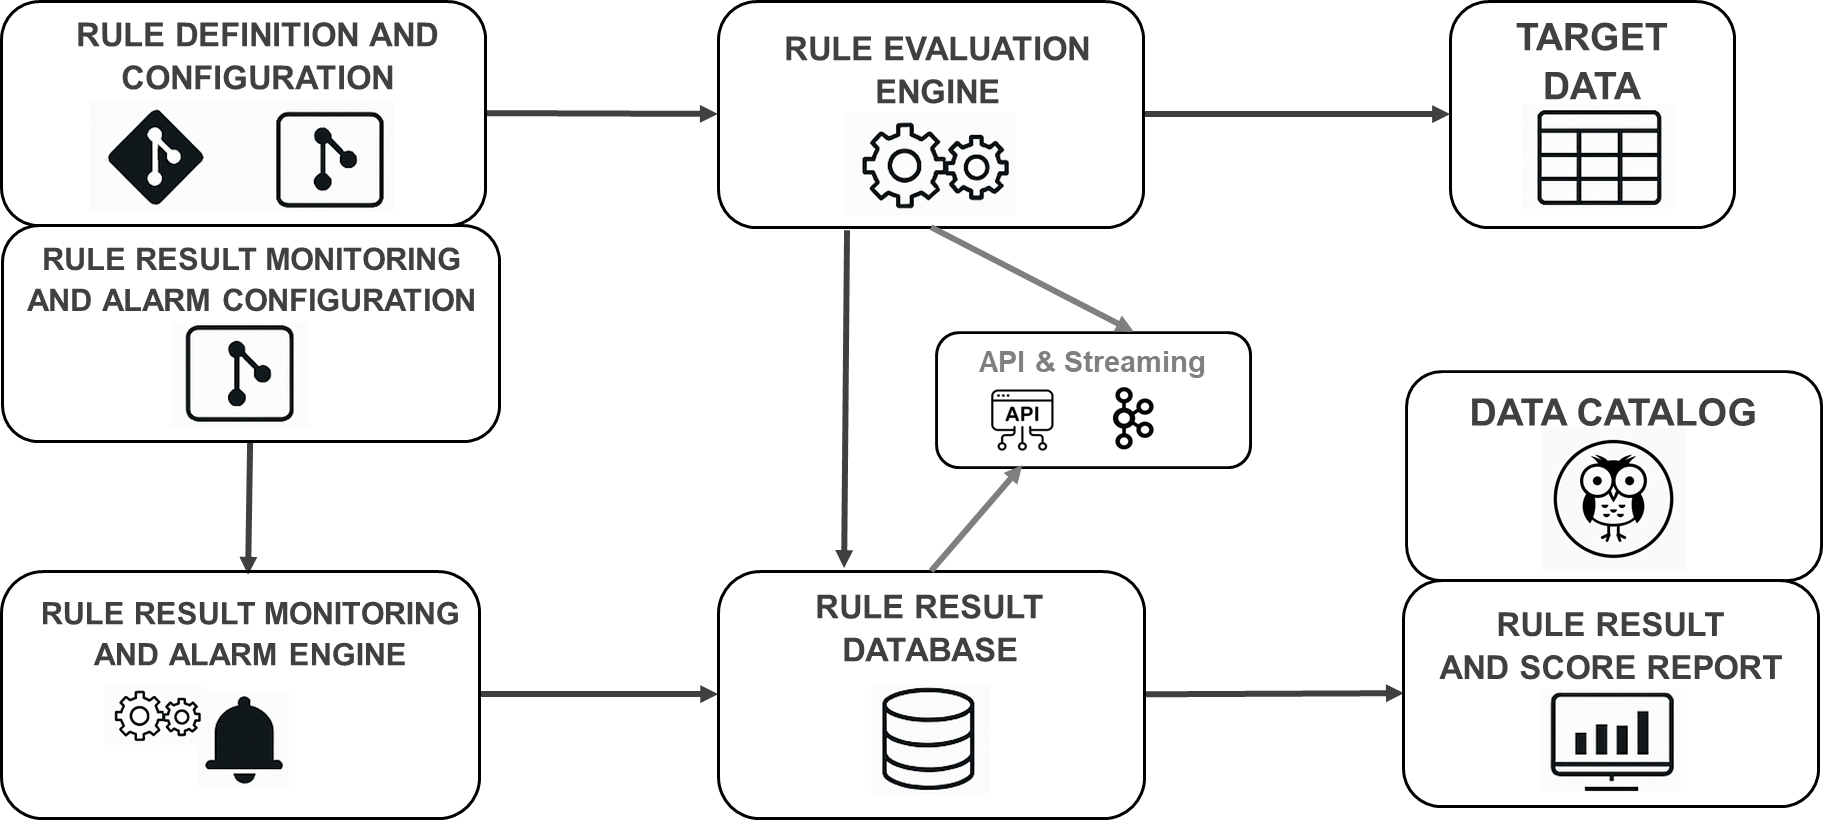
\includegraphics[width=0.8\textwidth]{./content/img/ProjectManagement/dqm_rules_architecture.png}
    \caption{The rule check engine architecture for future DQM}
    \label{fig:dwhlsops_kpi14_future_rulecheck_dqm}
\end{figure}



\subsection*{High-Level Target}
\label{SolutionDQMTeamHighLevelTarget}

From the complete target solution architecture, the first component to be implemented is a rule-based DQM suite. Its objective is to define generic data quality checks that can be applied across different datasets. This is achieved either by abstracting the check from the underlying data or by providing an SQL query that returns the data in a format allowing the same check to be applied to different datasets. The technology used to implement this solution is not discussed in this document, as the implementation was carried out by another team and is therefore outside the scope of this project. This approach consists of four main steps:

\begin{itemize}
    \item \textbf{Configuration}: Configuration defines the tables to be checked, the execution frequency, and the type of check.
    \item \textbf{Data preparation}: An SQL query prepares the data in a format suitable for the check.
    \item \textbf{Rule execution}: An application executes the defined checks on the prepared data.
    \item \textbf{Result persistence}: The results are stored in a database, which enables reporting.
\end{itemize}

\begin{figure}[H]
    \centering
    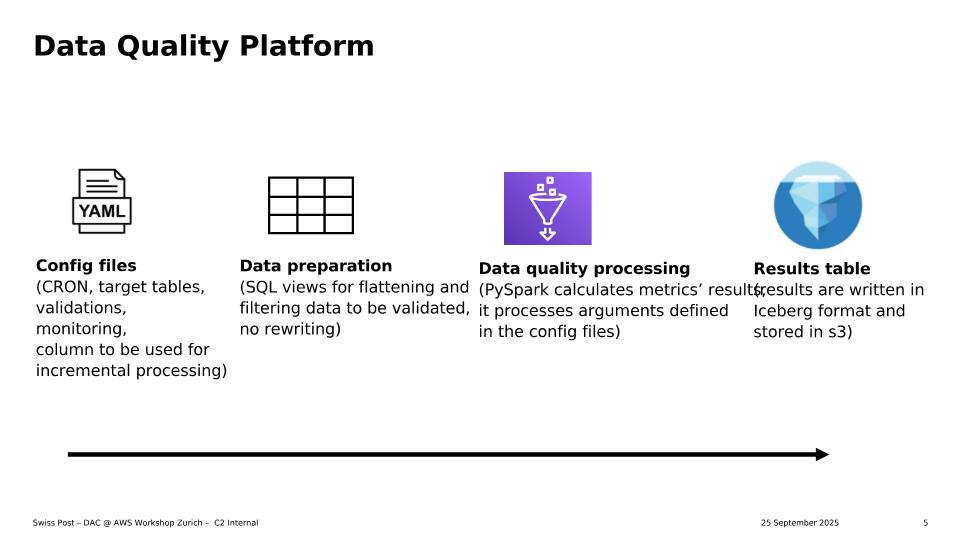
\includegraphics[width=0.8\textwidth]{./content/img/Solution_Design/Slide5.jpg}
    \caption{Intention of a DQM platform, high level}
    \label{fig:solutiondesign_slide5}
\end{figure}



\subsection*{Discarded Solutions}

This initiative is of high importance to the project, as it creates a major organisation-wide constraint to follow the \gls{DQM} team's choice of tool. The rationale for developing a rule-based DQM solution is that existing tools, such as \gls{AWSGlueDQ}, do not support views with complex data types, while \gls{PyDeequ} does not provide row-level results. These limitations in the evaluated tools led to the decision to develop a dedicated solution at Swiss Post, as described above. The following section provides a brief overview of the tools and approaches that were evaluated but ultimately discarded as unsuitable. The following screenshot shows the presentation in which the \gls{DQM} team summarised the evaluated tools and explained the reasoning behind their decision.


\begin{figure}[H]
    \centering
    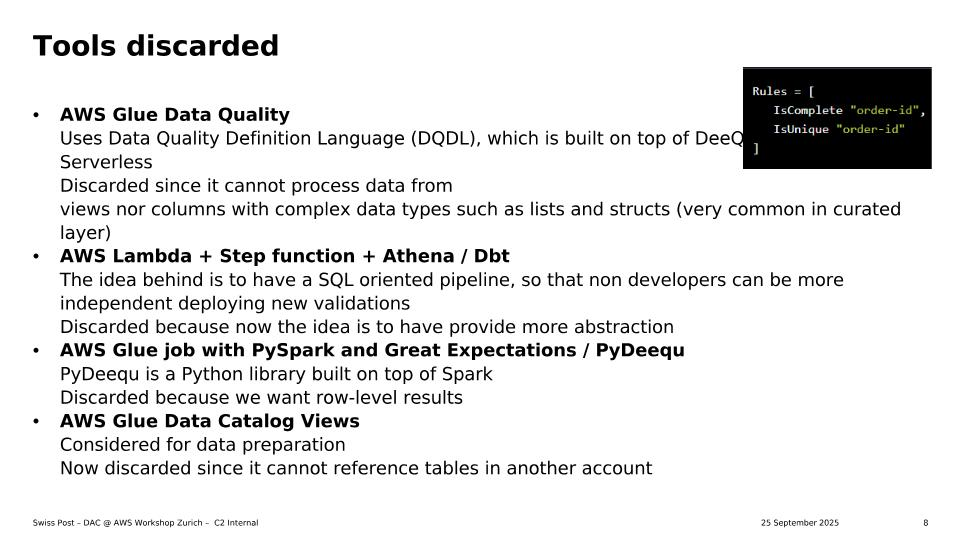
\includegraphics[width=0.8\textwidth]{./content/img/Solution_Design/Slide8.jpg}
    \caption{The list of tools discarded and the reasons for their exclusion}
    \label{fig:dwhlsops_kpi14_discarded_solutions}
\end{figure}

\subsection*{State at the end of this project}
\label{SolutionDQMEndOf2025}
By the end of 2025, the \gls{DQM} team set up a PoC of the rule check engine based on the design shown at the start of this section \ref{fig:dwhlsops_kpi14_future_rulecheck_dqm}. It allows running a check on a database view for specific target data source and storing the rule results in a designated rule result database. However many details were still not defined or implemented. Such as the location where the results check database is to be installed which has not been defined. Also the alerting and the setup of dashboards are currently out of scope, as are later additions such as deriving expected value ranges from historical data or holiday calendars. 



\section{Heterogenous sorting center environments}
\label{SolutionLandscapeMultHardWlayouts}
Before turning to the data lineage, an important constraint must be highlighted. The hardware used by Swiss Post in their high-tech “cyber” postal sorting centers differs in two main ways: across different providers and across different sizes and organisational structures of sorting centers. Which, in turn, also led to a diversity of processes to perform similar actions. This diversity on different levels brings certain benefits but also introduces additional synchronisation effort in other areas.

\subsection*{Different sorting hardware providers}
The hardware used by Swiss Post in its sorting centers is sourced from different providers. This is an essential risk management measure to reduce dependency on a single vendor. To mitigate this risk, Swiss Post decided to rely on at least two providers for essential hardware, not only to avoid dependency but also to protect against delivery issues or even the bankruptcy of individual providers. From a risk management perspective, this approach supports business continuity. However, from an IT perspective, it introduces challenges, as different hardware providers deliver data in different formats or with varying characteristics.

\subsection*{Different sorting center sizes and structure}
The Swiss Post parcel sorting centers are distinguished into two categories. There is one large \gls{PC} parcel center per \gls{region}, which is supplemented by smaller \gls{RPC} regional parcel centers. Regions encompass multiple cantons and may split cantons into the four current regions: west, middle, east, and south. The organisation into larger parcel centers and smaller regional parcel centers helps to optimise processes and reduce the carbon footprint of postal services. However, each PC and RPC differs from the others.

First, due to differences in size, processes differ between small and large centers, and the way of work also varies as organisational structures are different. Second, beyond the distinction between small and large centers, each center has a unique layout. Third, tasks can differ between centers; for example, some also handle letters. While these differences are reasonable from an operational perspective, they introduce challenges for centralised reporting, where all variations need to be harmonised. The following figure shows selected PC and RPC locations distributed across Switzerland.

\begin{figure}[H]
    \centering
    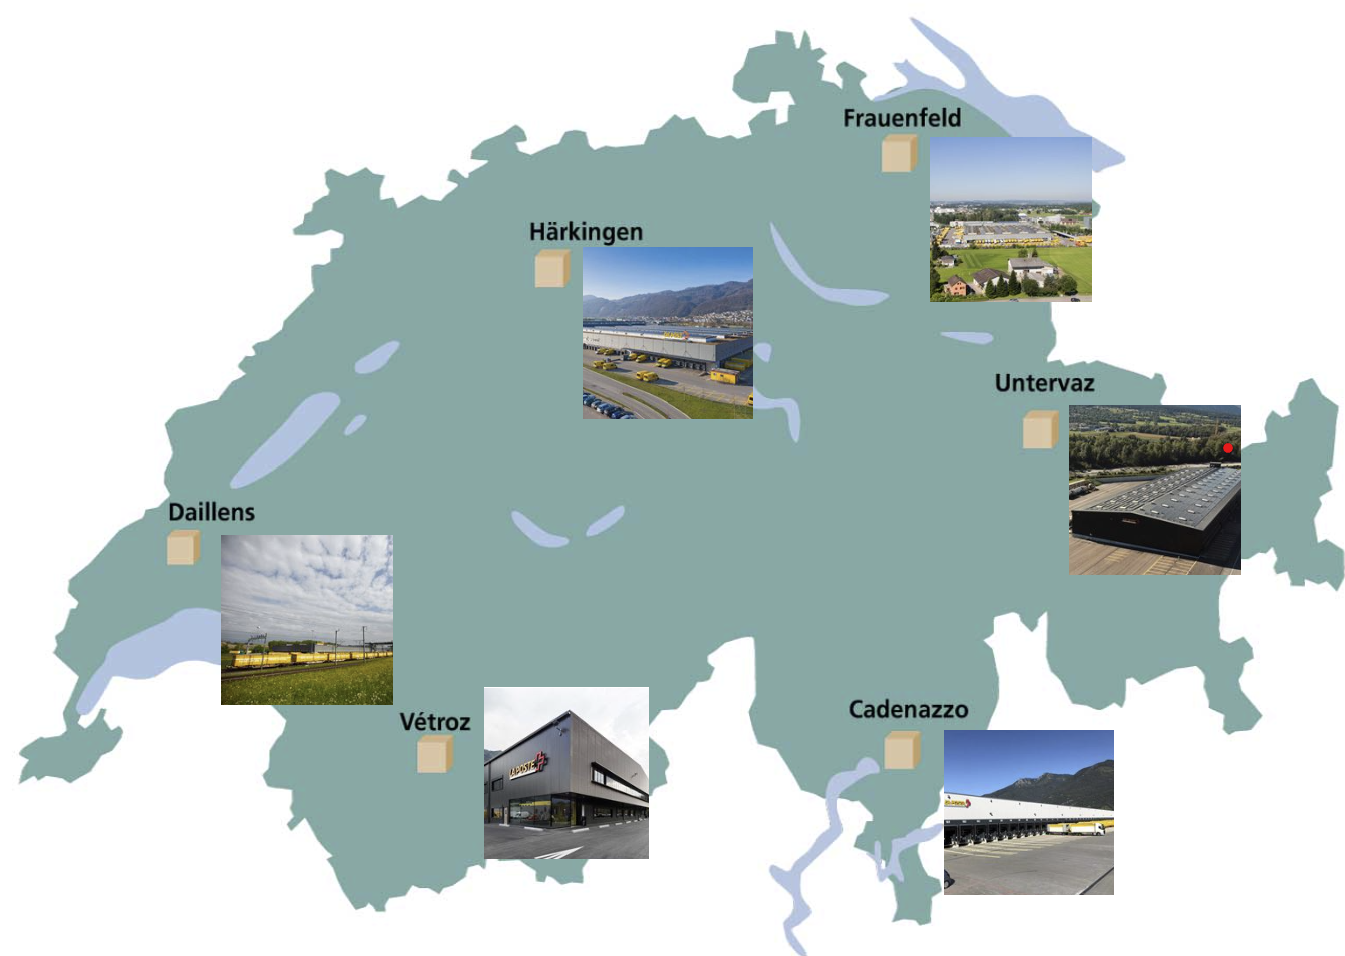
\includegraphics[width=0.8\textwidth]{./content/img/Solution_Design/PZ_RPZ_Schweiz_Edit.png}
    \caption{Selection of parcel sorting centers distributed over Switzerland}
    \label{fig:design_PC_and_RPC}
\end{figure}

\subsection*{Different sorting processes}
\label{SolutionLandscapeLayoutsDiffProcess}
To go one step further, the different size and equipment at the sorting centers lead to different actions performed in the sorting centers. The same event in a sorting center can be caused by different previous actions making reporting on them difficult. As an example, the submitted and discharged events are described further.

\subsubsection*{Submitted event}
\label{SolutionSubmittedEvent}
The submitted event is the first automatic scan that occurs after a mail piece is placed onto the automatic sorting machine. In the context of this project, a mail piece refers to a parcel. However, parcels are not always placed onto the sorting machine in the same way. This can occur via roll boxes (\gls{RX}), which are automatically emptied by robots. An RX is a container, as depicted in the following figures, that is used to transport different mail pieces through sorting and delivery facilities. Alternatively, parcels can be placed onto the automatic machine manually by staff, either by removing them from RX units or by emptying truck containers onto conveyor belts, as shown in the subsequent figures.

\begin{figure}[H]
    \centering
    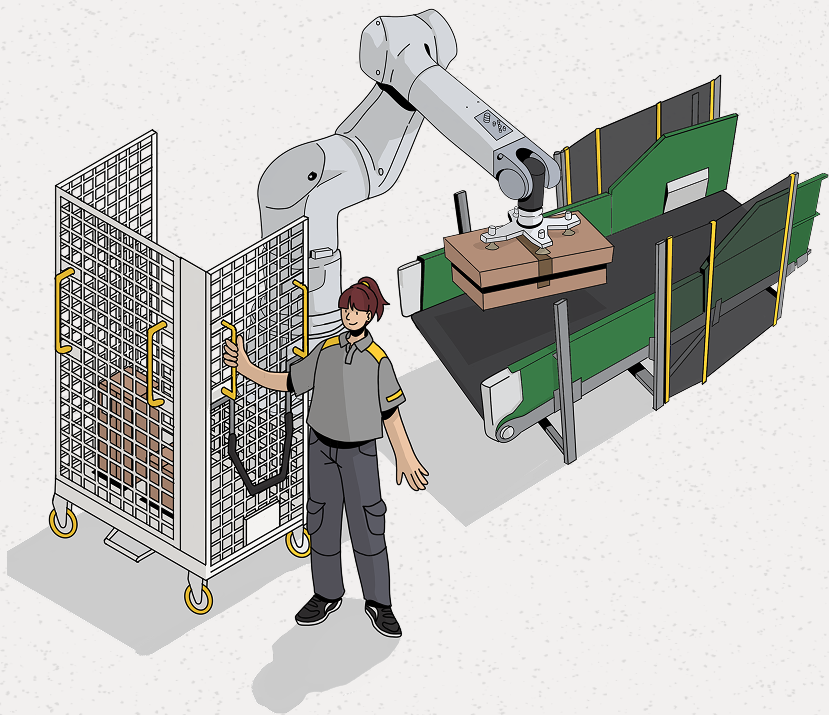
\includegraphics[width=0.8\textwidth]{./content/img/Post_internal/Visual_Subm_PostGraphic_02_12_2025.png}
    \caption{Parcel sorting, parcels submitted by robot}
    \label{fig:submitting_robot}
\end{figure}
\begin{figure}[H]
    \centering
    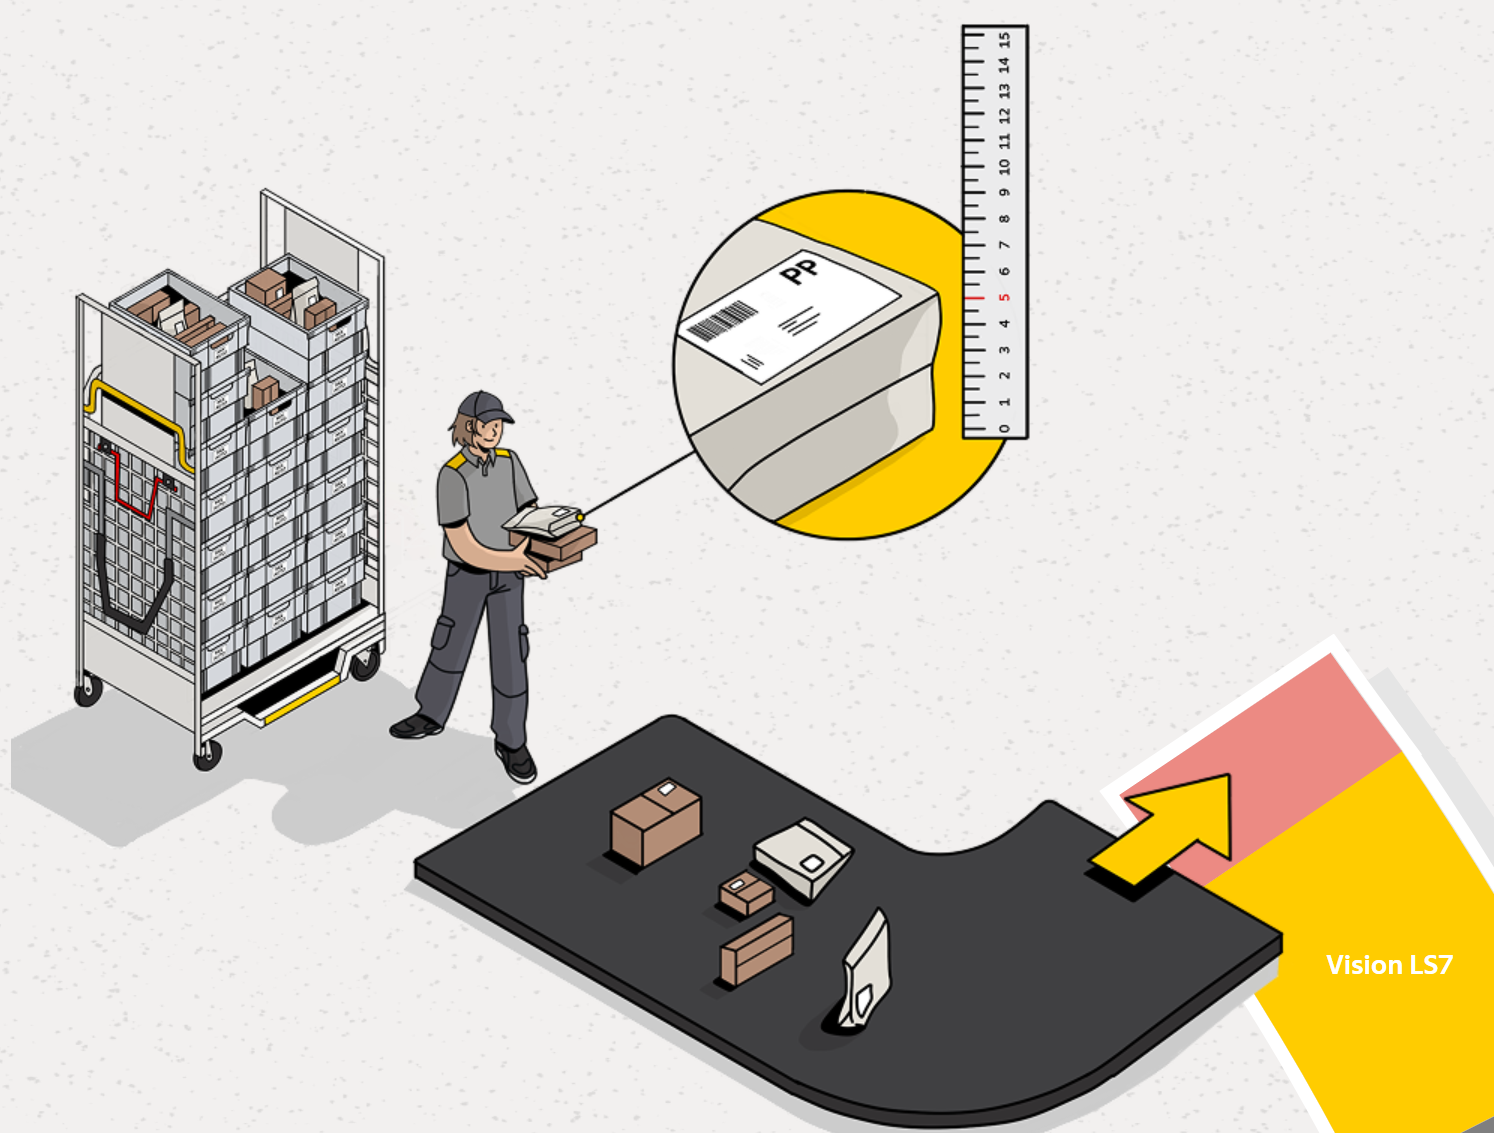
\includegraphics[width=0.8\textwidth]{./content/img/Post_internal/Visual_Subm1_PostGraphic_02_12_2025.png}
    \caption{Parcel sorting, smaller items submitted manually}
    \label{fig:submitting_small_manual}
\end{figure}
\begin{figure}[H]
    \centering
    \includegraphics[width=0.8\textwidth]{./content/img/Post_ExperienceHub/_DSC4856.jpg}
    \caption{Manual parcel onloading from a truck}
    \label{fig:Solution_manual_truck_unload}
\end{figure}

\subsubsection*{Discharged event}
\label{SolutionDischargedEvent}
The discharged event is complementary to the submitted event. It is the last automatic scan event of a parcel when it leaves the automated sorting machine. This can happen in different ways, such as when the parcel is discharged via a chute where staff load it into an RX, when it is discharged directly into an RX automatically by the machine, or when it is automatically ejected after completing a defined number of cycles through the machine. All of these possibilities trigger different follow-up actions. However, in all mentioned cases, a discharged scan is performed after the parcel is removed from the automatic sorting machine. This is the important aspect for reporting, as these two events (submitted and discharged) occur once per complete cycle that a parcel runs through the automatic sorters.

\begin{figure}[H]
    \centering
    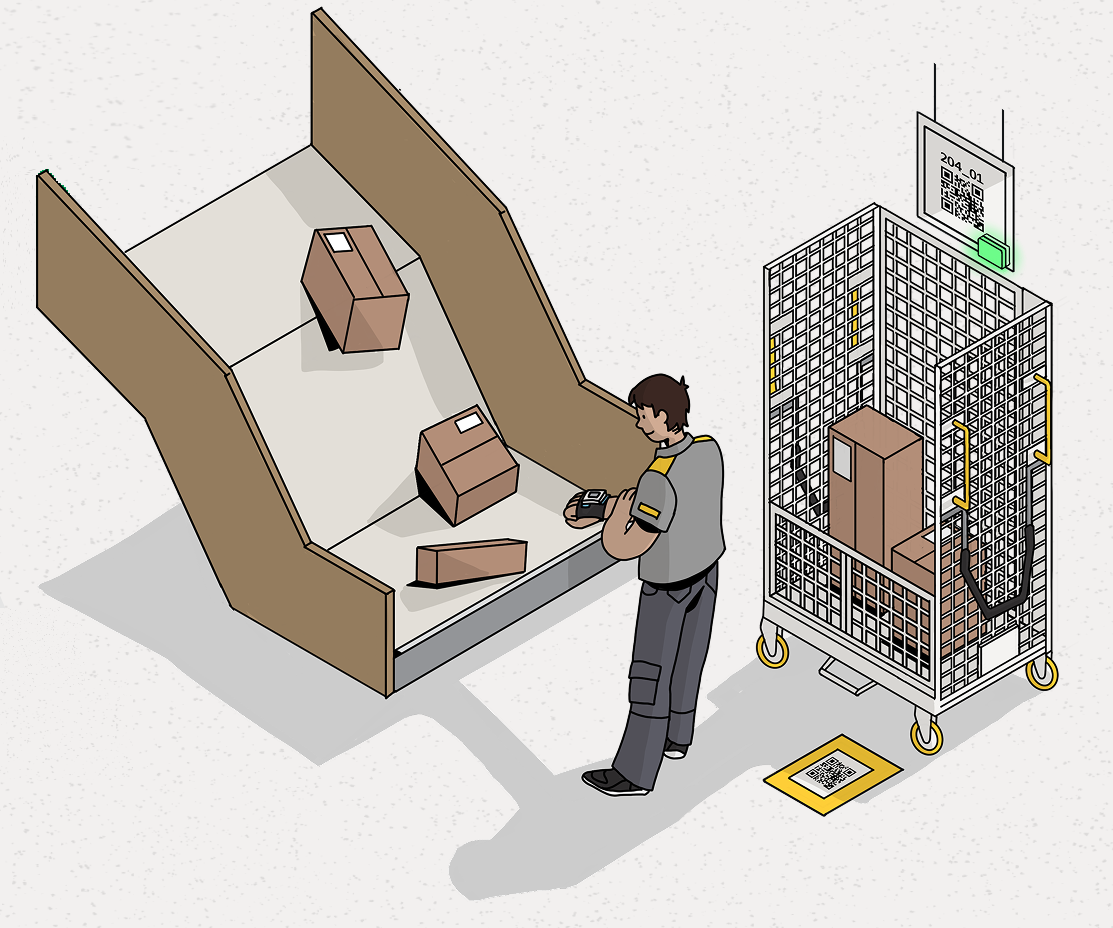
\includegraphics[width=0.8\textwidth]{./content/img/Post_internal/Visual_DisCh_PostGraphic_02_12_2025.png}
    \caption{Parcel discharged, manual loading into RX}
    \label{fig:discharged_manual_visualisationl}
\end{figure}



\section{Data Lineage}
\label{SolutionDataLineage}

The data relevant to this project are those used by the DWH LS OPS team. They consist of cleaned and deduplicated data stored in the \gls{curated} database layer. However, these data originate from sensor data and arrive in the data warehouse (\gls{DWH}) in a raw format. Before reaching the curated layer, the data pass through four main processing steps, which are also shown in the following figure:

\begin{itemize}
    \item \textbf{Physical data source}: Parcels are scanned by different scanners in the sorting centres. As described above, Swiss Post uses a variety of devices from different hardware vendors, which naturally results in a large number of data entities that must be stored. Each parcel passes through multiple scanners during its journey across the Swiss Post's 13 sorting centres, generating multiple data entities that are transferred to the data warehouse. Determining the exact number of generated events was outside the scope of this project.
    \item \textbf{Initial data storage}: The scan events are first saved in AWS S3.  At first glance this might be a very unusual choice, but the reasons make sense. First, the Swiss Post has a cloud strategy which includes AWS as a service provider; hence the choice of AWS is no surprise.  But more importantly, Amazon S3 (Simple Storage Service) is the object storage service of AWS. Exactly which data are stored here and how is addressed in a following section.
    \item \textbf{Kafka ingestion}: Apache Kafka is an open-source distributed event streaming platform designed for high-throughput, fault-tolerant, real-time data pipelines and event-driven architectures.The Swiss Post 
[ operates a Kafka environment in its down data centers ]
[ uses the Amazon MSK Managed Streaming for Kafka ].
With this,  so-called “producers” read the data from the initial storage and ingest it into Kafka “topics,” to which other systems can “subscribe” and obtain the data.

    \item \textbf{Data delivery to DWH}: Kafka consumers ingest the events into the DWH LS OPS raw data layer. Which is the first storage layer in this teams AWS S3 account, saving the data as recieved from Apache Kafka. 
\end{itemize}

\begin{figure}[H]
    \centering
    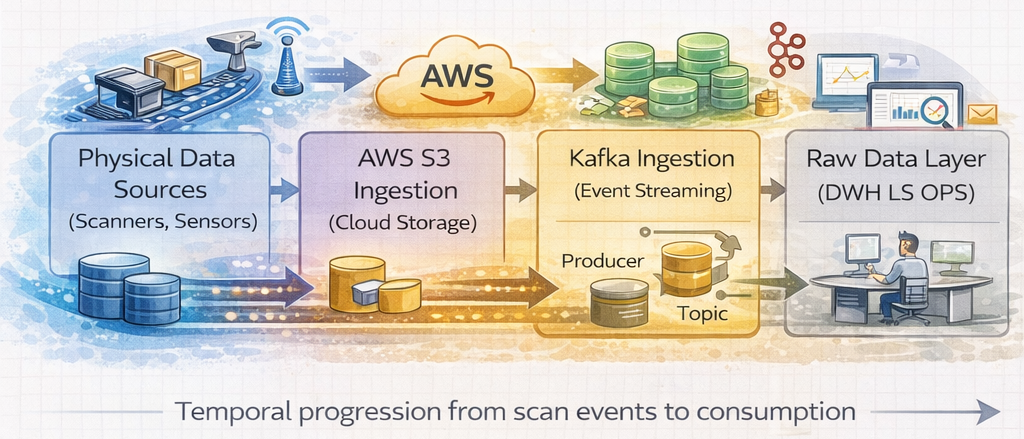
\includegraphics[width=0.8\textwidth]{./content/img/Solution_Design/DataLineage_ChatGPT_generated_MainSteps.png}
    \caption{An artistic high-level view of the DWH LS OPS data lineage}
    \label{fig:design_Datalineage_paintedGPT_beforeDWH}
\end{figure}

\textbf{KEY POINT:}  From the data creating stage until  the data arrives at the DWH, it passes through four IT system steps discussed here. This results in four potential sources of failure, in which each system is counted only once and by ignoring different possible errors per step. This landscape makes it difficult to trace errors that can occur at any step. Additionally, the variety of errors is large, as they may alter data values or result in no data being transmitted at a given step, even though the operation of the sorting center itself continues without issues. Therefore, at a technical level, providing clarity especially during the operational aspect is an important key aspect of this project.

Finally, to complete the picture of the data lineage, one more step is relevant. After the data has arrived in the raw layer at DWH LS OPS, it must be cleaned and deduplicated. At this step, differences in hardware providers and the structural differences of sorting centers come into effect, and the unification of the data takes place. All of this is performed in the step towards the curated database layer, after which a reporting layer serves as the final layer from which reporting tools retrieve data as introduced in chapter \ref{subsec:ResearchReportingPipeline}. This is illustrated here with a focus on the central step from the raw layer to the curated layer. Even after the curated layer, there is one additional layer, namely the reporting layer. 

The different layers in the cloud are set up according to a structure similar to that used in the classical on-premises DWH at Swiss Post. This similarity to the on-premises DWH stems from deliberate architectural alignment. The cloud infrastructure was built with the guidance of on-premises developers using their domain knowledge. In this way, functional and structural consistency was maintained, as the architecture continues to follow the Kimball star schema and the layered architecture as defined in the Kimball technical architecture \cite{KimballTechnicalArchitecture}.

\begin{figure}[H]
    \centering
    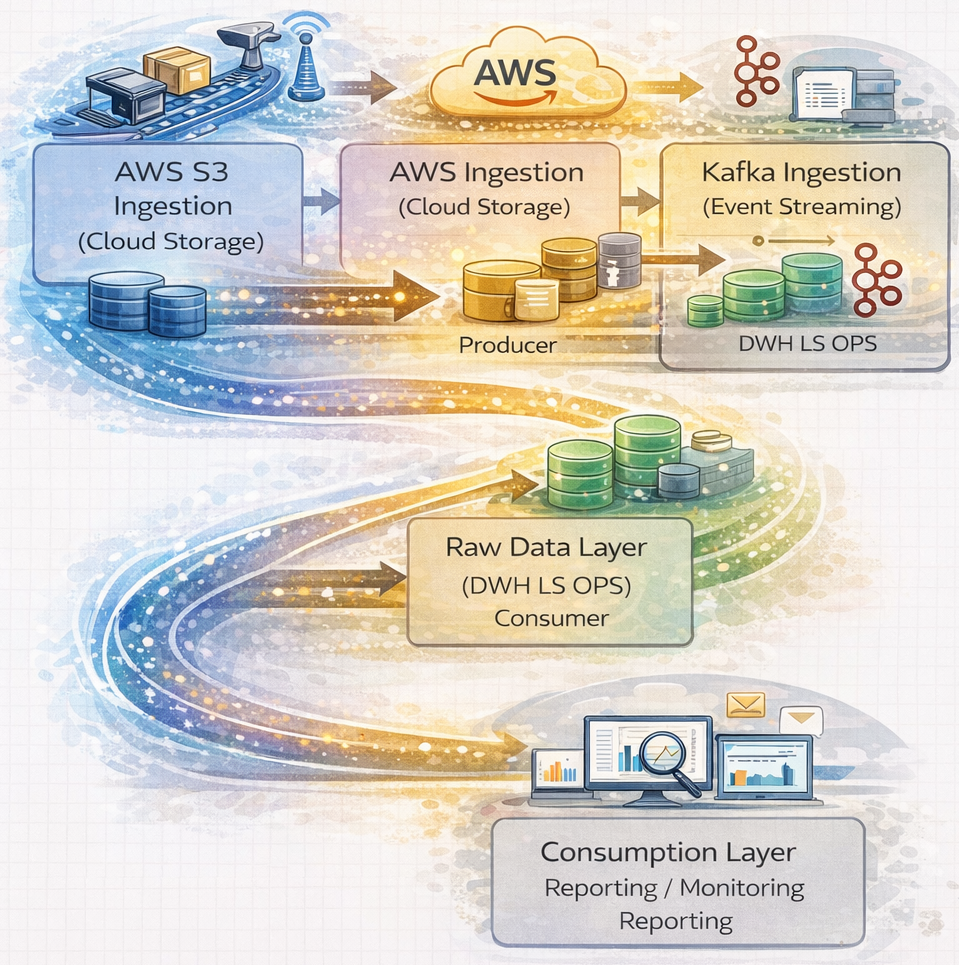
\includegraphics[width=0.8\textwidth]{./content/img/Solution_Design/DataLineage_ChatGPT_completer_view.png}
    \caption{An artistic high-level view of the full DWH LS OPS data lineage up to reporting}
    \label{fig:design_Datalineage_paintedGPT_full_tillReporting}
\end{figure}


\section{This project as a key step towards the “future state” reporting solution}
\label{SolutionIntentedSol}

As stated earlier the solutional goal of this project and its follow up is to provide an MVP for DQM, from which the key learnings will enable the full “future state” reporting solution. This MVP should implement an automatic data quality check, replacing an occasional, non automated check performed by the business. This is important, as the DQM check is currently executed by the business instead of IT, which creates challenges with regard to the desired target state. The expected situation would be that IT executes data quality checks and defines thresholds together with the business. At present, however, the knowledge about thresholds and other relevant information resides solely with the business.

In summary, having IT run the data checks would enable continuous follow-up of data quality. For example, a report based on automatically executed checks could show system uptime over a longer period of time. This information would later allow IT to extrapolate standard value ranges, which in turn would enable the definition of alerting thresholds. In short, having DQM checks executed automatically rather than occasionally by the business provides multiple benefits for both IT and the business.

\begin{figure}[H]
    \centering
    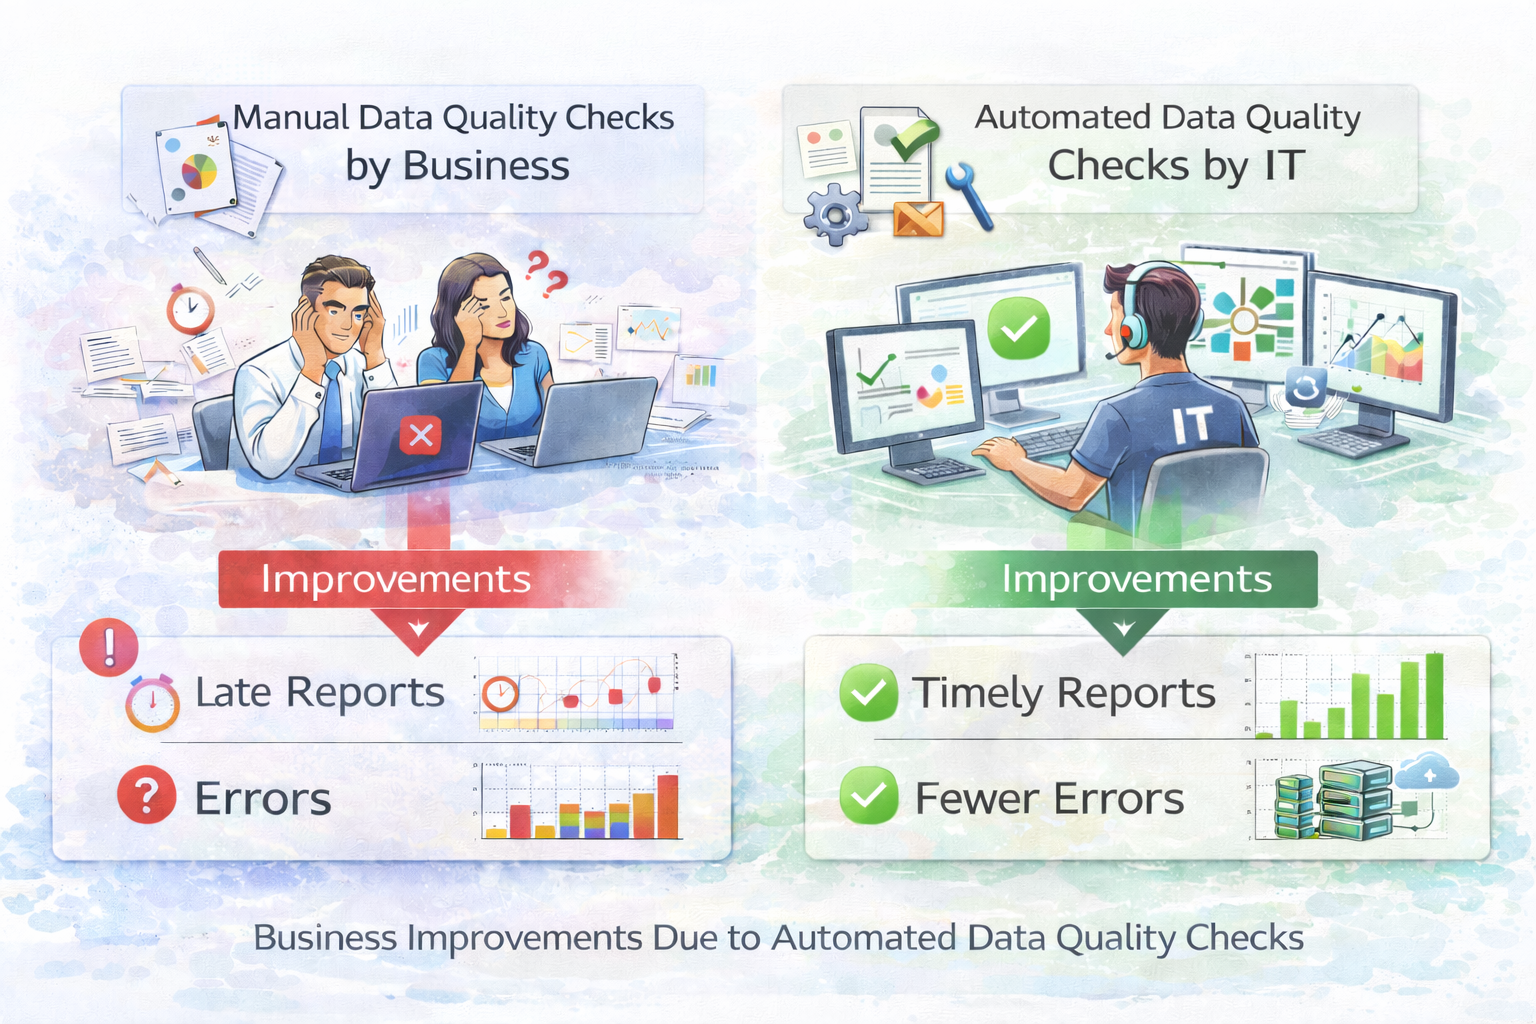
\includegraphics[width=0.8\textwidth]{./content/img/Solution_Design/businessChecks_against_ITautomated.png}
    \caption{DQM manual checks against automated checks by IT}
    \label{fig:dqm_manual_automated}
\end{figure}


\section{Expected benefits of this reporting solution}
\label{SolutionReasonsForSol}
A single visualisation does not explain the full benefit of the intended solution. For instance, the question arises as to why the business should stop performing data quality checks when it has the most detailed knowledge of the data. This is quickly clarified by taking a step back. The question should not be why checks are removed from the business, but why the reports are performed by the business in the first place. The benefits of this shift are therefore outlined in more detail in the following.

\subsection*{Benefit 1: Automation over manual processes to reduce effort}
\label{SolutionReasonsAutomationOverManual}
The business currently spends 30 to 45 minutes per day on a single data quality check, according to the initial project hand in description. From the duration of the check, it can be inferred that anyone requiring the data quality check before a report based on it is approved must wait until it is finished, resulting in a waiting time of 30 to 45 minutes. This fact provides the basis for understanding why manual processes are not suitable at scale. When scaling up to ten data quality checks, five to seven and a half hours are spent by the business on data quality checks. The waiting time for the last reports to be approved increases accordingly to five to seven and a half hours. When increasing to 20 checks per day, ten to 15 hours are spent, and the waiting time rises accordingly, accounting for more than one full-time position and long delays in report data release. It should be noted that this amount of time is spent solely to determine whether the defined check passes or not.
If the same initial check is executed by an automated data quality process, the expectation is that execution takes less than one minute; for simplicity, an execution time of one minute is assumed. As no manual initiation is required, no human time is spent performing the check. For comparison, the one minute waiting time for report approval and release is still considered. The business can then be informed whether the check returned an OK or not OK result, and the outcome can be stored for future reference.

When scaling this approach to ten checks, the total execution time remains ten times one minute. However, as the IT system can execute these checks in parallel, the waiting time for results remains at one minute. When increasing to 20 checks per day, the IT systems likewise execute the checks in parallel, and the execution and waiting time remain unchanged.

\subsubsection*{Benefit 2: Scalability to further reduce overall time required}
In summary, manual data quality checks cannot be scaled and lead to excessive use of human resources for repetitive tasks, as well as long waiting times for approved datasets. Automated data quality checks, by contrast, allow many checks to be executed in parallel within the same overall time frame. It should be noted that this comparison assumes all checks have similar complexity.

\subsection*{Benefit 3: Rule changes without query changes}
The current manual reports, which are business driven, have their logic built directly into the queries executed on the data. If any rule changes or a part of the data processing is modified, these queries need to be adapted. Thus, the check is deeply tied to the data source. To illustrate this with an example, a data quality check may confirm that 30\% of the data is category A and 70\% is category B, as this is considered the expected and valid distribution. If changes to processing pipelines or client behaviour cause the share of A to increase to 45\% and B to decrease to 55\%, the query performing the check must be adapted. However, when the check is performed by an application that injects these thresholds into a query, the query itself does not need to change, and only the parameters must be adjusted.

\subsubsection*{Benefit 4:  Reusability to improve stability and performance}
By moving the responsibility for checks from manual, business-driven processes to automated checks executed by IT, the checks can be designed to be more generic. Generic checks can be reused across different use cases. This separation of responsibilities and concerns leads to improved stability and performance when applying the checks, which in turn enables strong reusability. The same check type can be applied to different data sources by adapting parameters such as the query and thresholds, while the underlying check logic remains unchanged.



\section{Existing reporting pipeline}
\label{SolutionReportingPipeline}
The current reporting pipeline at DWH LS OPS team consists of four main components as shown in following figure and introduced in chapter \ref{subsec:ResearchReportingPipeline}. First, the storage layer (in figure : \textbf{Datenspeicherung}), where data is retrieved, cleaned, and saved to \gls{AWSS3}. Second, the query and processing layer, where cleaned data is queried using Amazon \gls{athena} and \gls{DSP}(in figure : \textbf{Datenselektierung, Datenpreparation Datenmodelle Data Federation}), and where data is passed and persisted in data models for reports. Third, the reporting and consumption layer, in which data from DSP is used in \gls{SAC} reports (in figure : \textbf{Business Layer}).

\begin{figure}[H]
    \centering
    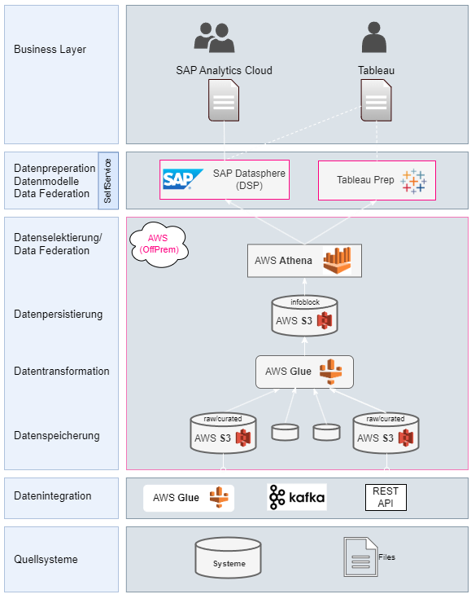
\includegraphics[width=0.8\textwidth]{./content/img/Solution_Design/DWH_CloudSTructure_OnlyHW.png}
    \caption{The DWH LS OPS reporting layers}
    \label{fig:Solution_Landscape_cloud_layers}
\end{figure}

\subsubsection*{AWS S3}

As described by Amazon: \textit{“Amazon Simple Storage Service (Amazon S3) is an object storage service that offers industry-leading scalability, data availability, security, and performance. Customers of all sizes and industries can use Amazon S3 to store and protect any amount of data for a range of use cases, such as data lakes, websites, mobile applications, backup and restore, archive, enterprise applications, IoT devices, and big data analytics. Amazon S3 provides management features so that you can optimize, organize, and configure access to your data to meet your specific business, organizational, and compliance requirements.” \cite{aws_s3_docs}.}

This is relevant for Swiss Post, as Amazon S3 serves as the central storage for data from mail piece events, which include all scans of parcels and mail in sorting centers, as well as later stages up to the delivery process. This storage is used by the DWH LS OPS team. All data entering the data lineage pipeline, for example through Kafka or through direct database connections, is stored in Amazon S3. Thus, it represents the first persistence point in the reporting pipeline.

\paragraph{Layered architecture}
It is important to note that the data is not only initially saved to Amazon S3 in a raw layer, but is also cleaned and prepared for reporting in two additional layers. To separate the storage of raw data from the cleaning process, multiple layers are used. This ensures that all data in its original format is saved first before processing, modification, augmentation, and checks for completeness or correctness are performed. Each step can therefore be reproduced and repeated, which is useful whenever data needs to be reloaded, for example when data was incomplete for a day or when new processing methods are developed.
After the raw layer, data is deduplicated and cleaned, and then saved into the curated layer. The final top layer, the reporting layer, mainly adds translations of fields into business terminology, for example by changing column labels. This is useful for the business, as it enables consistent naming of columns across tables or data products. 

\paragraph{Infoblock}
\label{SolutionLandscapeInfoblock}
On this level \gls{infoblock}'s are generated, this is a Swiss Post internal term used for report ready data products. An infoblock is cleaned, deduplicated, curated data which features joined datasets that use business naming, e.g. \gls{postday} and processing, priority types. Basically the infoblocks are the final layer employed on the reporting layer, making them accessible to the reporting tools such as \gls{DSP} and \gls{SAC}, which are described in detail below. A more comon term for infoblock know trough out the industry is data product  \cite{alation_data_product, ibm_data_product}. 

\subsubsection*{AWS Athena query}
\label{SolutionAthenaQuery}
The next step is Amazon Athena as the query layer, which Amazon describes as follows: \textit{ “Amazon Athena is an interactive query service that makes it easy to analyze data directly in Amazon Simple Storage Service (Amazon S3) using standard SQL. With a few actions in the AWS Management Console, you can point Athena at your data stored in Amazon S3 and begin using standard SQL to run ad-hoc queries and get results in seconds. “ \cite{aws_athena_docs}.}
Amazon Athena is used by Swiss Post DWH LS OPS for all queries on Amazon S3, which is the next step in the reporting pipeline. Athena is the tool designed by AWS for use with S3, making it the logical choice for querying the stored data. The data is queried for reporting purposes by selecting the relevant subsets.

\paragraph{DQM relevance}
The querying layer is relevant to DQM, since data quality issues may become apparent first at this earliest checkpoint, for example when errors occur in the data itself and counts or joins become invalid. While the data is queried at this layer for reporting purposes, it is also queried here for data quality checks. Such checks typically address missing data and data completeness, but can also extend to data plausibility, for example when postal codes are compared to cities. In cases where issues occur at this layer, they are passed downstream towards DSP and SAC, provided they do not already break the pipeline at this stage.


\subsubsection*{SAP products SAP Datasphere (DSP) and SAP Analytics Cloud (SAC)}
At Swiss Post, the next step in the reporting pipeline uses the two dependent tools SAP Datasphere (DSP) and SAP Analytics Cloud (SAC). These are described as follows by SAP:

\textit{SAP Datasphere enables organizations to combine, harmonize, and model data from multiple SAP and non-SAP sources within a semantically rich, cloud-based data environment. 
SAP Analytics Cloud can directly consume these governed and business-ready data models via live connections, enabling interactive reporting, analytics, planning, and forecasting. 
In addition, planning and forecast data created in SAP Analytics Cloud can be written back to SAP Datasphere, allowing analytical and planning data to coexist in a single, integrated data foundation \cite{sap_datasphere_sac_integration}.}

SAP Datasphere (DSP) is SAP’s cloud-based data platform for integrating, modeling, and analyzing data across SAP and non-SAP systems while preserving business semantics. It enables federated access to distributed data without full replication and supports end-to-end data lineage and governance. DSP at Swiss Post is used as the analytical backbone for reporting, analytics, and data-driven decision-making in SAP landscapes.

SAP Analytics Cloud (SAC), in turn, uses the data model provided by DSP to present this information on the business layer to end users. More information on this is provided in the separate section introducing the tool.


\subsubsection*{DSP datamodel}
\label{SolutionDesignDSPModel}
After querying, the data is persisted in \gls{DSP}, where it is made available in data models. This persistence and processing layer is essential in the current pipeline, as data can be made available to \gls{SAC} only through DSP. At Swiss Post, data persistence has proven essential to improving the response time of the reporting pipeline as a whole.
 With this persistence, DSP does not pass queries back to Amazon Athena, creating a clear separation between the two layers. Due to this separation, DSP is not responsible for DQM, which is handled in lower layers. Finally, DSP is the layer in which business logic is applied in a semantic form, defining what the data represents. At Swiss Post, this is done by applying business oriented naming and calculations. Different report consumers may require the same values to be structured in different ways; for example, productivity in a sorting center may be measured using total working hours against the number of mail pieces handled, or calculated using only time spent on sorting-related tasks, excluding breaks, training, and other activities.
 
\paragraph{DSP use case}
The data models in DSP are useful not only as a bridge to SAC (discussed below). They allow different data sources to be modelled and combined into unified data models. This is also relevant to Swiss Post, as it operates not only Amazon Athena data sources but also other database- or file-based sources. This combination of data inevitably inherits data quality issues from the underlying sources, which can affect joins, data loading, and further processing. Nonetheless, DSP is the sole source of data provided to SAC, which is the next logical step in the reporting pipeline. This also means that any unhandled data quality issues are passed directly to users consuming reports in SAC and may therefore affect confidence in the reporting pipeline depending on data quality.

\subsubsection*{SAP Analytics Cloud (SAC) report}
SAC is the final step in the reporting pipeline and represents the reporting and consumption layer. As the last layer, it inherits the data from previous layers and is responsible only for its visualisation. The data is displayed passively, and no further transformations are performed at this stage. Consequently, any errors in data preparation or data quality issues from upstream layers are propagated to this layer together with the data itself.

As described earlier, SAC is dependent on DSP and cannot operate independently, nor does it provide native DQM capabilities. The reports generated by SAC are therefore fully dependent on the preceding layers, and any issues or delays are reflected directly in the reports. This is particularly relevant for Swiss Post, as one report provided by DWH LS OPS is used daily at 07:00 for shift handover, which takes place one hour after the end of the \gls{postday}. Some data sources required for this report become available only after 06:00, the end of the postday. If any upstream step is delayed, the report delivery is delayed accordingly.

\paragraph{Consumption layer}
As the consumption layer for reports, this is the point at which users with read access have their first and only interaction with the reporting pipeline. It is at this stage that user confidence is either established or lost, making it particularly critical. Users do not see the upstream processing steps and typically do not differentiate whether missing or delayed information is caused by AWS S3, Athena, or DSP.

\section{Report visualisations and evaluations}
After the basic solution landscape this project now dives deeper into the more specific context of report visualisations and evaluation of automatisation.



\subsection*{Power BI}

At Swiss Post in the environment of the \gls{DWHLSOPS}, \gls{PowerBI} is the set business intelligence tool. It is to replace the currently used tools over time. The main reasons for this shift are the lower license cost in comparision with the previous \gls{SAC} and furthermore it has performed faster in direct comparision tests with its predesessor. Therefore, Power BI served as BI tool in this project, as it is specifically replacing an old report in \gls{SAC}.
\subsubsection*{Architectural position}
When considering the data lineage, Power BI is replacing both the \gls{DSP} on the data model side, as well as the front end part of \gls{SAC}. So in total it is replacing the work areas of the business stakeholders coworking with the \gls{DWHLSOPS} team. This is so because they are involved both in the generation of testing and updating the reports on the reporting and monitoring layer.



\subsection*{Star shema}
During the speed tests and comparisions with the old business intelligence tool, the star shema as a data architecture was tested. It showed that \gls{PowerBI} was performing better with this new structure. Therefore as Power BI was designated as new business intelligence tool, the architecture was changed to this.

\subsubsection*{Basic architectureof star shema}
When looking at data base architecture, a star shema is basically a partly denormalised database which has been optimised for fast \gls{OLAP} processing. In computing, online analytical processing (OLAP), is an approach to quickly answer multi-dimensional analytical (MDA) queries. This describes the ground work that reporting has to perform in the \gls{DWHLSOPS} team.

A star shema is described by wikipedia in the following way \cite{enwiki:1306074452}:
\begin{quote}
\textit{In computing, the star schema or star model is the simplest style of data mart schema and is the approach most widely used to develop data warehouses and dimensional data marts. The star schema consists of one or more fact tables referencing any number of dimension tables. The star schema is an important special case of the snowflake schema, and is more effective for handling simpler queries.
The star schema gets its name from the physical model's resemblance to a star shape with a fact table at its center and the dimension tables surrounding it representing the star's points.}
\end{quote}


\subsubsection*{Basic architectureof Wide table}
In contrast to a star shema, a wide table is storing all the data in one big, very wide table. This concept of \gls{widetable} was introduced at Swiss Post, together with \gls{SAC}. In a wide table, the data is not split in different tables, but instead for every dataset all measures existing are repeated. For example every data point measurement that happened at the same factory, would have the same identifying measures of an address repeated rather than only 1 key pointing to a adresses table.

A short concise description of the concept can be found at  \cite{enwiki:QuestDBWideTable}:
\begin{quote}
\textit{
Wide tables are the opposite of narrow tables, storing multiple related attributes horizontally rather than vertically. In time-series applications, a wide table typically has a timestamp column followed by numerous metric columns, making it efficient to retrieve multiple metrics for a given time point.}
\end{quote}



\subsection*{Reporting idea}
When considering the previous report generated trough \gls{SAC}, it can be seen that is is not very visual. The data is only shown as a table without color highlights or additional indications. Without sufficient business knowhow it did not allow a user to see wether the data quality was ok or not for a specific day. The current report is shown in the following.
\begin{figure}[H]
    \centering
    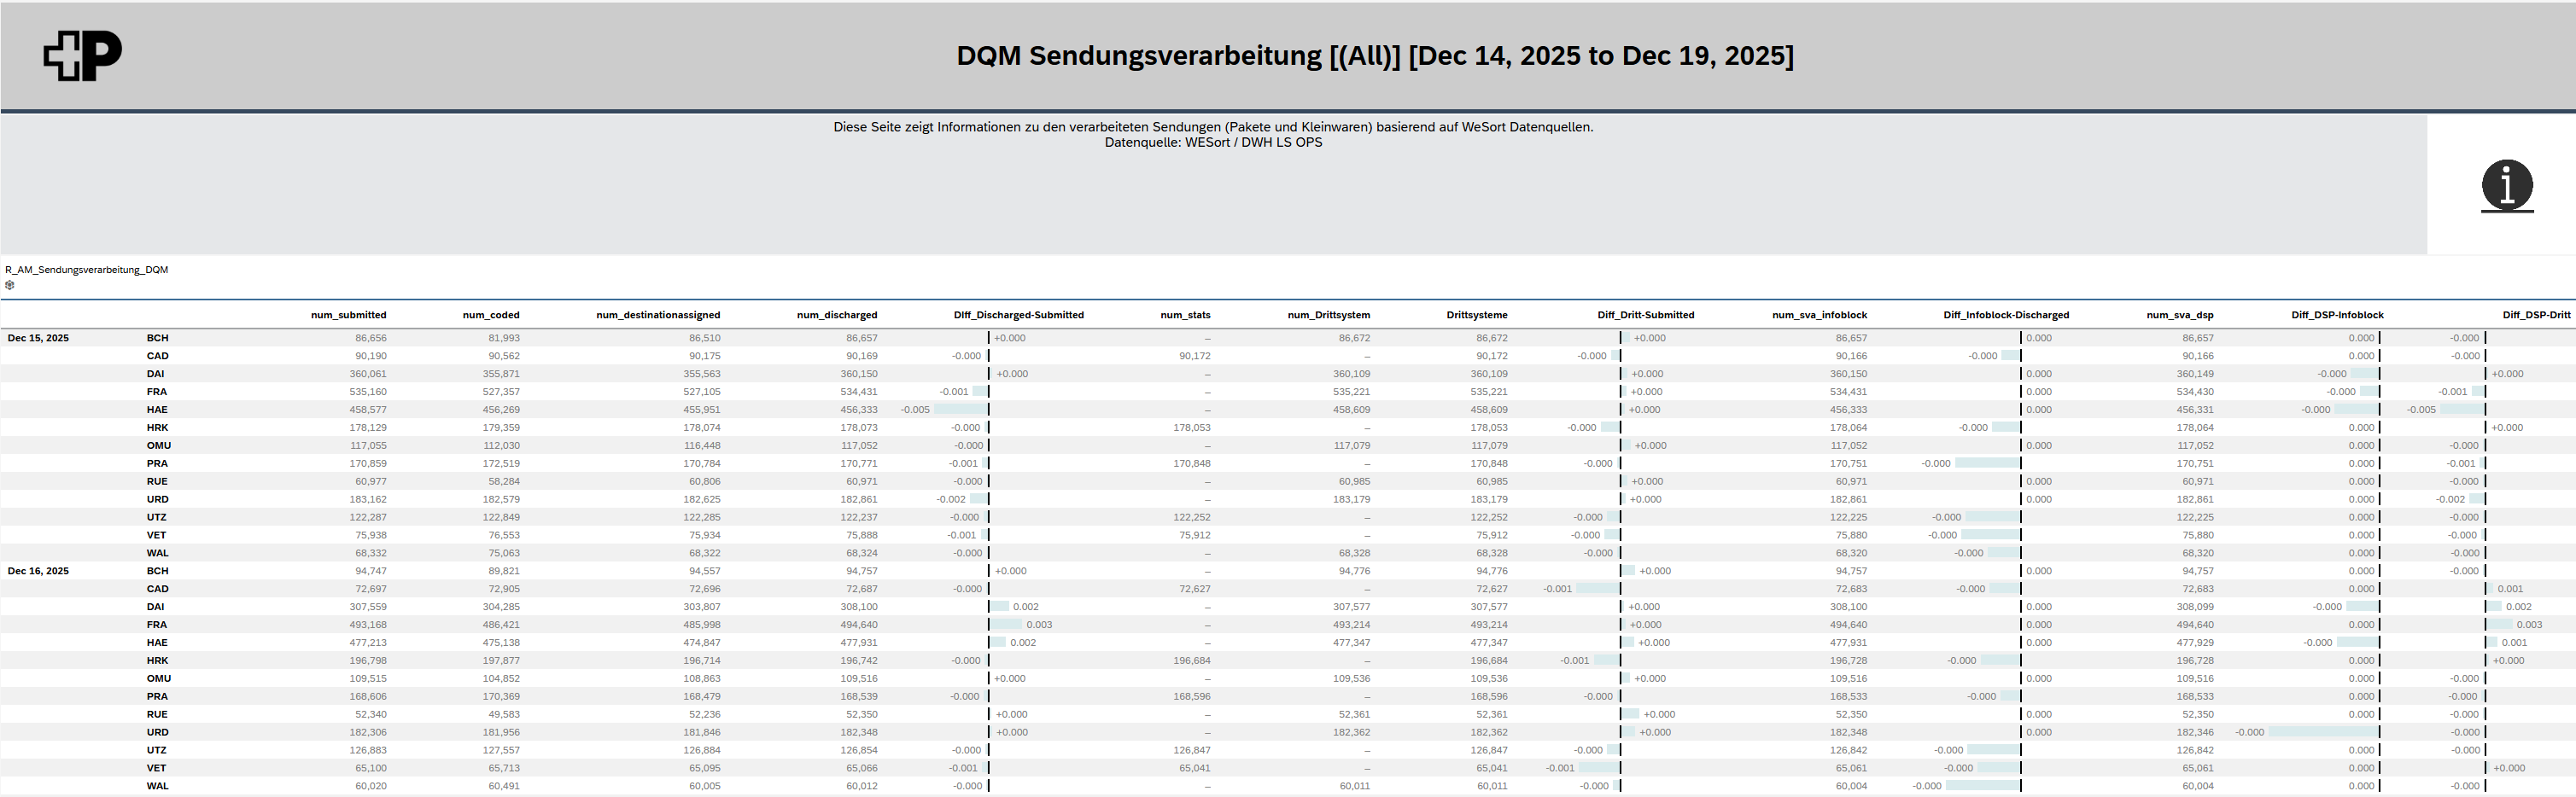
\includegraphics[width=0.95\textwidth]{./content/img/Plain_DQM_WEST_19-12-2025_08-43-34.png}
    \caption{Existing plain DQM dashboard used as the baseline for the redesigned Power BI report}
    \label{fig:plain_dqm_dashboard}
\end{figure}

To improve this situation, a report which hast to replace it, must be more visual. And apply some of the most basic business knowledge allowing to see its results faster. As the previous research has already defined which rules must be applied in an automatic check, those rules are the basis for the reports visualisation.

\subsubsection{Business stakeholder feedback}
During meetings with the business their requirements were accumulated. Those were simple, the report had to be upgraded to use the new data source. Since with the adoption of Power BI, also a more efficient reporting datastructure was possible, it had to be again measurable. As the data itself was only rearranged but not radically new, the checks and the way they had to be shown in a table stayed the same. Regarding additional improvements of the report no direction was given, however an OK was provided to improve the report with useful information.



\subsection*{DevOps}
At Swiss Post deployments are done by the software engineers effectively turning their field of operations to \gls{DevOps}. 

The field of DevOps is described by Wikipedia as follows \cite{enwiki:1362982395}:
DevOps is the integration and automation of software development and information technology operations. DevOps encompasses the tasks necessary for software development and can lead to both shortening development time and improving the development life cycle. According to American software architect Neal Ford, DevOps, particularly through continuous delivery, employs the "bring the pain forward" principle by tackling challenging tasks early, fostering automation, and enabling swift issue detection.

Although debated, DevOps is generally characterized by three key principles: shared ownership, workflow automation, and rapid feedback. From an academic perspective, Len Bass, Ingo Weber, and Liming Zhu—three computer science researchers from the CSIRO and the Software Engineering Institute—defined DevOps as "a set of practices intended to reduce the time between committing a change to a system and the change being placed into normal production, while ensuring high quality". However, the term is used in multiple contexts. At its most successful, DevOps is a combination of specific practices, culture change, and tools.



\subsubsection*{DevOps at Swiss Post}
At Swiss Post this the DevOps process is already defined and is not changed by this project, it will apply all defined tools and rules. To name the general rules:


\begin{itemize}
    \item GitHub is used as CodeRepository using SSO with post accounts
    \item The access to repositories is limited and managed by a permission system
    \item Separate repositories exist for development and productive environments
    \item Repositories are also separated by function, e.g. repositories for teraform \gls{IaC} or sql scripts for \gls{athena}
    \item Development is performed on branches
    \item To merge branches a pull request is required, this triggeres GitHub actions
    \item The Github actions are performing checks depending on repository and function
    \item To merge code on production environments a review by another developer is required in addition to successful Github actions
    \item In addition to this deployment pipeline, DevOPS engineer continue maintaining and support their code
\end{itemize}



\subsubsection*{Frontend deployment pipelines}

Regarding frontend reports a similar process is already defined and also applie, not adapted by this project.
When deploying front end reports using Power BI, the process is happening entirely on the microsoft environments.
\begin{itemize}
    \item Reports are initially created on Power BI desktop
    \item Development and testing happens on the desktop version first
    \item The report is deployed from Power BI desktop to Microsoft Fabric, development environment
    \item The code is checked in using git integration in Microsoft 
    \item The report is tested first in the development environment
    \item Then it is deployed trough the defined pipeline to test environment
    \item Stakeholders are performing tests on test environment
    \item After successful tests and eventual fixes the go for productive deployment is given
    \item Productive deployment is done again trough the deployment pipeline
\end{itemize}

The deployment pipeline is shown in the below figure, showing the selection of environments from which the 3 steps process starts.

\begin{figure}[H]
    \centering
    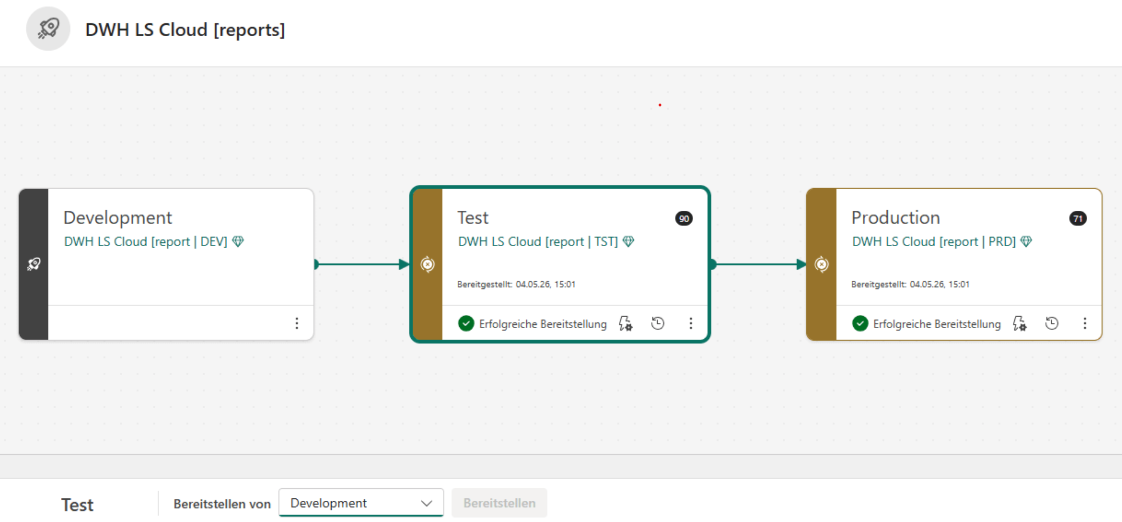
\includegraphics[width=0.95\textwidth]{./content/img/PowerBI_Deployment.png}
    \caption{Power BI deployment pipeline across the development, test, and production environments}
    \label{fig:powerbi_deployment_pipeline}
\end{figure}



\section{DQM tool selection}
The DQM tool selection required a structured approach. Such approach required to first setup a list of requirements towards a tools. Then a evaluation how well tools are fulfilling these requirements. And finally the invitation of the fulfilling providers to demos.

\subsection*{Tool selection principles}
the first step in evaluating a tool must be to get to know, what a tools actually needs to have. Commonly those lists are called requirement lists.
They have to incorporate the must have features of a tool and the nice to have requirements. With such a list, the decision together with higher management is made easier, as they allow for a scoring and easy overview of which tool scored how many points. Based on such points list, the per performing or best price can be selected.

\subsection*{Requirements list}
At Swiss Post the \gls{DQM} team setup the requirements list. It incorporates the following main principles:

\begin{itemize}
    \item \textbf{Data Coverage \& Connectivity:} The integration into the existing tool landscape. The requiements to be cloud first. Most important data sources that need to be handled.
    \item \textbf{Data Quality Capabilities:} What actual DQM requirements the tool must fullfill. The usability which is expected, such as NoCode environments.
    \item \textbf{Reporting \& Monitoring:} The tool must allow exports to other tools for reporting purpose.
    \item \textbf{Performance and Reliability:} The tool needs to be responsive also on big datasets as Swiss Post will want to run checks on very large transaction datasets.
    \item \textbf{Cost \& Licensing:} The cost of a tool is relevant. How is the cost structured.
\end{itemize}

\begin{figure}[H]
    \centering
    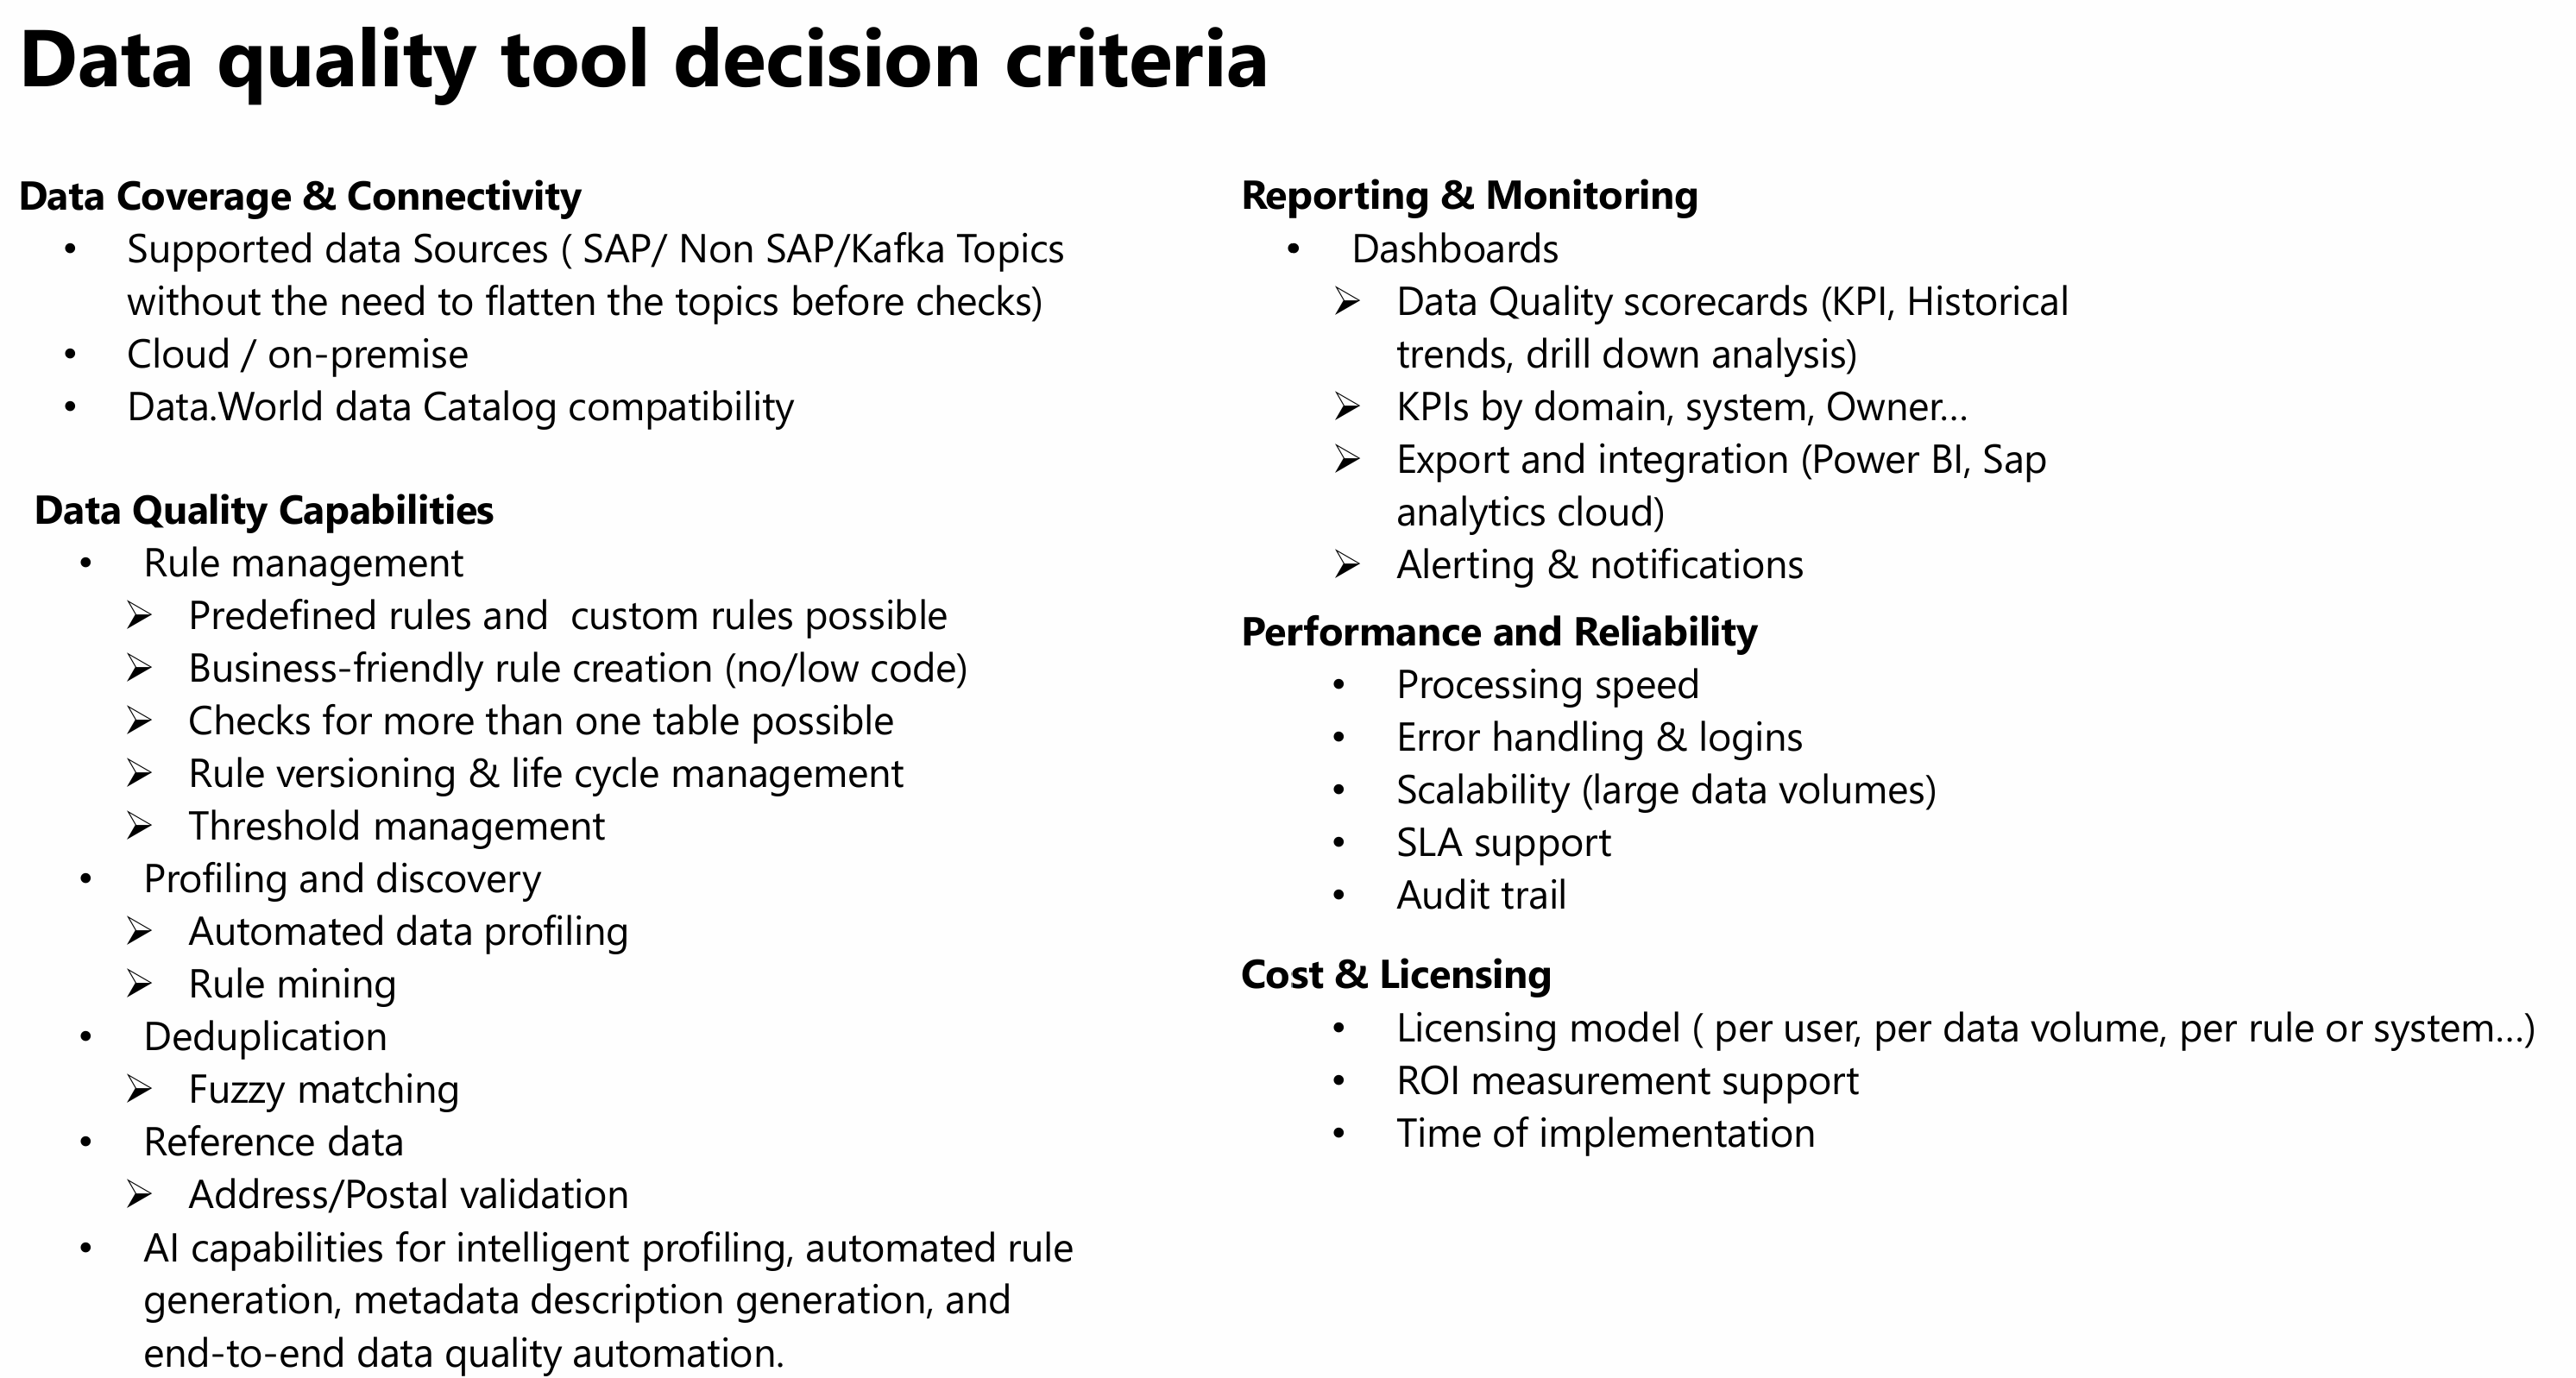
\includegraphics[width=0.95\textwidth]{./content/PostInput1/DQM_Tool_Evaluation_1.png}
    \caption{Overview of the data quality management tool evaluation process and the assessed evaluation criteria}
    \label{fig:dqm_tool_evaluation_1}
\end{figure}

Additionally there are the more \gls{softcriteria} which are nice to have. Soft criteria are the criteria which are not mandatory but make the usage of an application easier for users e.g. provide easy management of access roles. The list as defined by Swiss Post is shown in the following screenshot:

\begin{itemize}
    \item \textbf{Usability \& User experience:} User permission system allowing multiple different access levels and their provisioning trough existing means.
    \item \textbf{Technical requirements:} The security requirements which the cloud solution has to meet. Additionally the connectivity options they need to support
\end{itemize}

\begin{figure}[H]
    \centering
    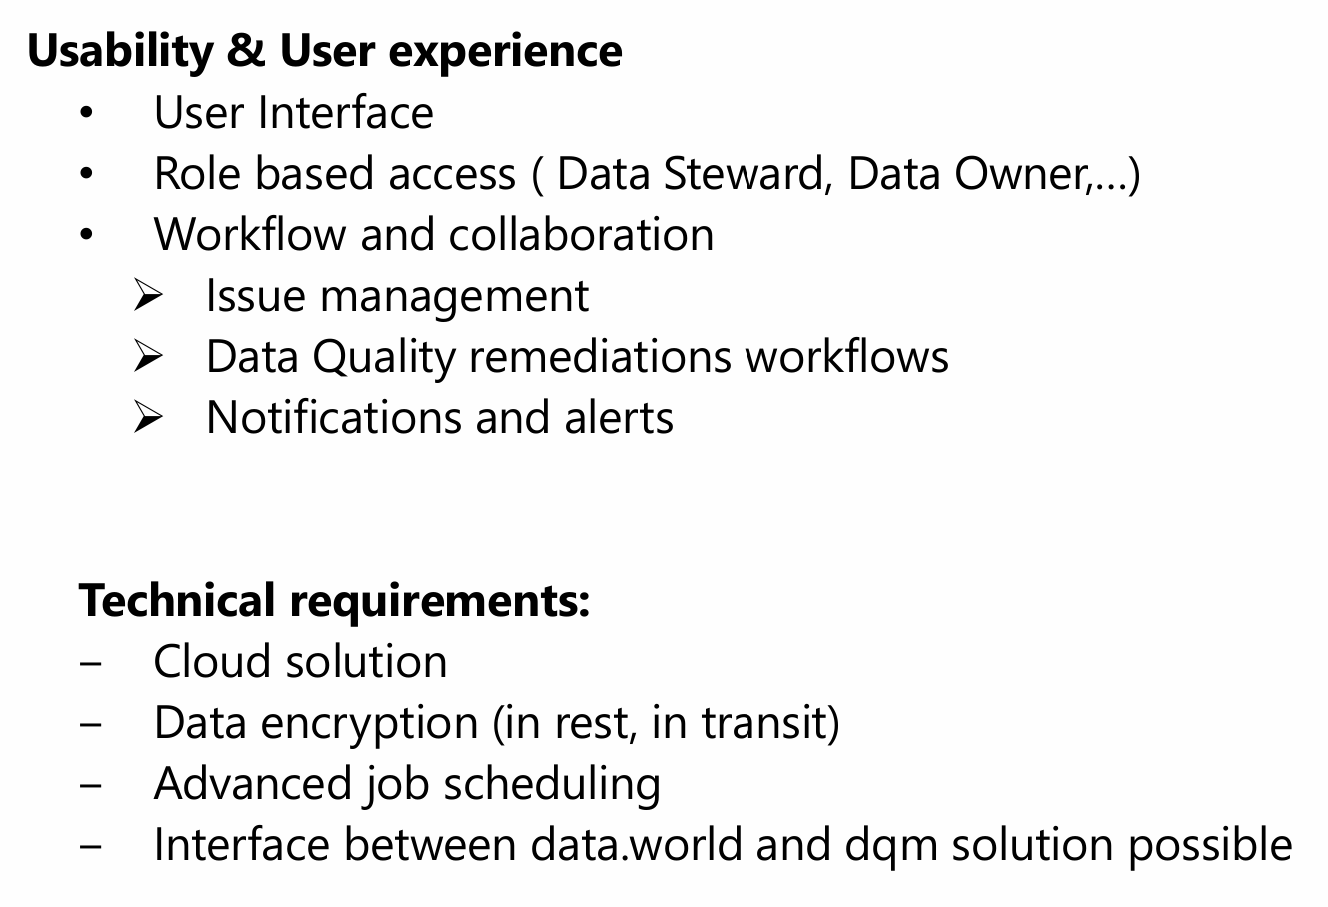
\includegraphics[width=0.45\textwidth]{./content/PostInput1/DQM_Tool_Evaluation_2.png}
    \caption{Continuation of the data quality management tool evaluation, including the comparison of the evaluated solutions}
    \label{fig:dqm_tool_evaluation_2}
\end{figure}

\subsection*{DQM tooling selection}
After having the selection criteria, the tools are researched. The research of these tools has also been done by the DQM team so its out of scope for this work.
As a result of the tool research, the different found tools are evaluated against the criteria. This finally results in the table as shown below highlighting the performance of the tools against criteria. This table the serves for which tools are inivited for demos or directly excluded. The following screenshots shows the five tools which made it into the evaluation, including the tree in green which were invited for demos.

\begin{itemize}
    \item \textbf{Ataccama ONE} : Selected for demo
    \item \textbf{Informatica IDMC (CDQ + optional Streaming)} : Selected for demo
    \item \textbf{Soda (Core + Cloud)} : Selected for demo. The demo is documented later in the document.
    \item \textbf{Great Expectations} : Not selected for demo
    \item \textbf{SAP Information Steward} : Not selected for demo
\end{itemize}


\begin{figure}[H]
    \centering
    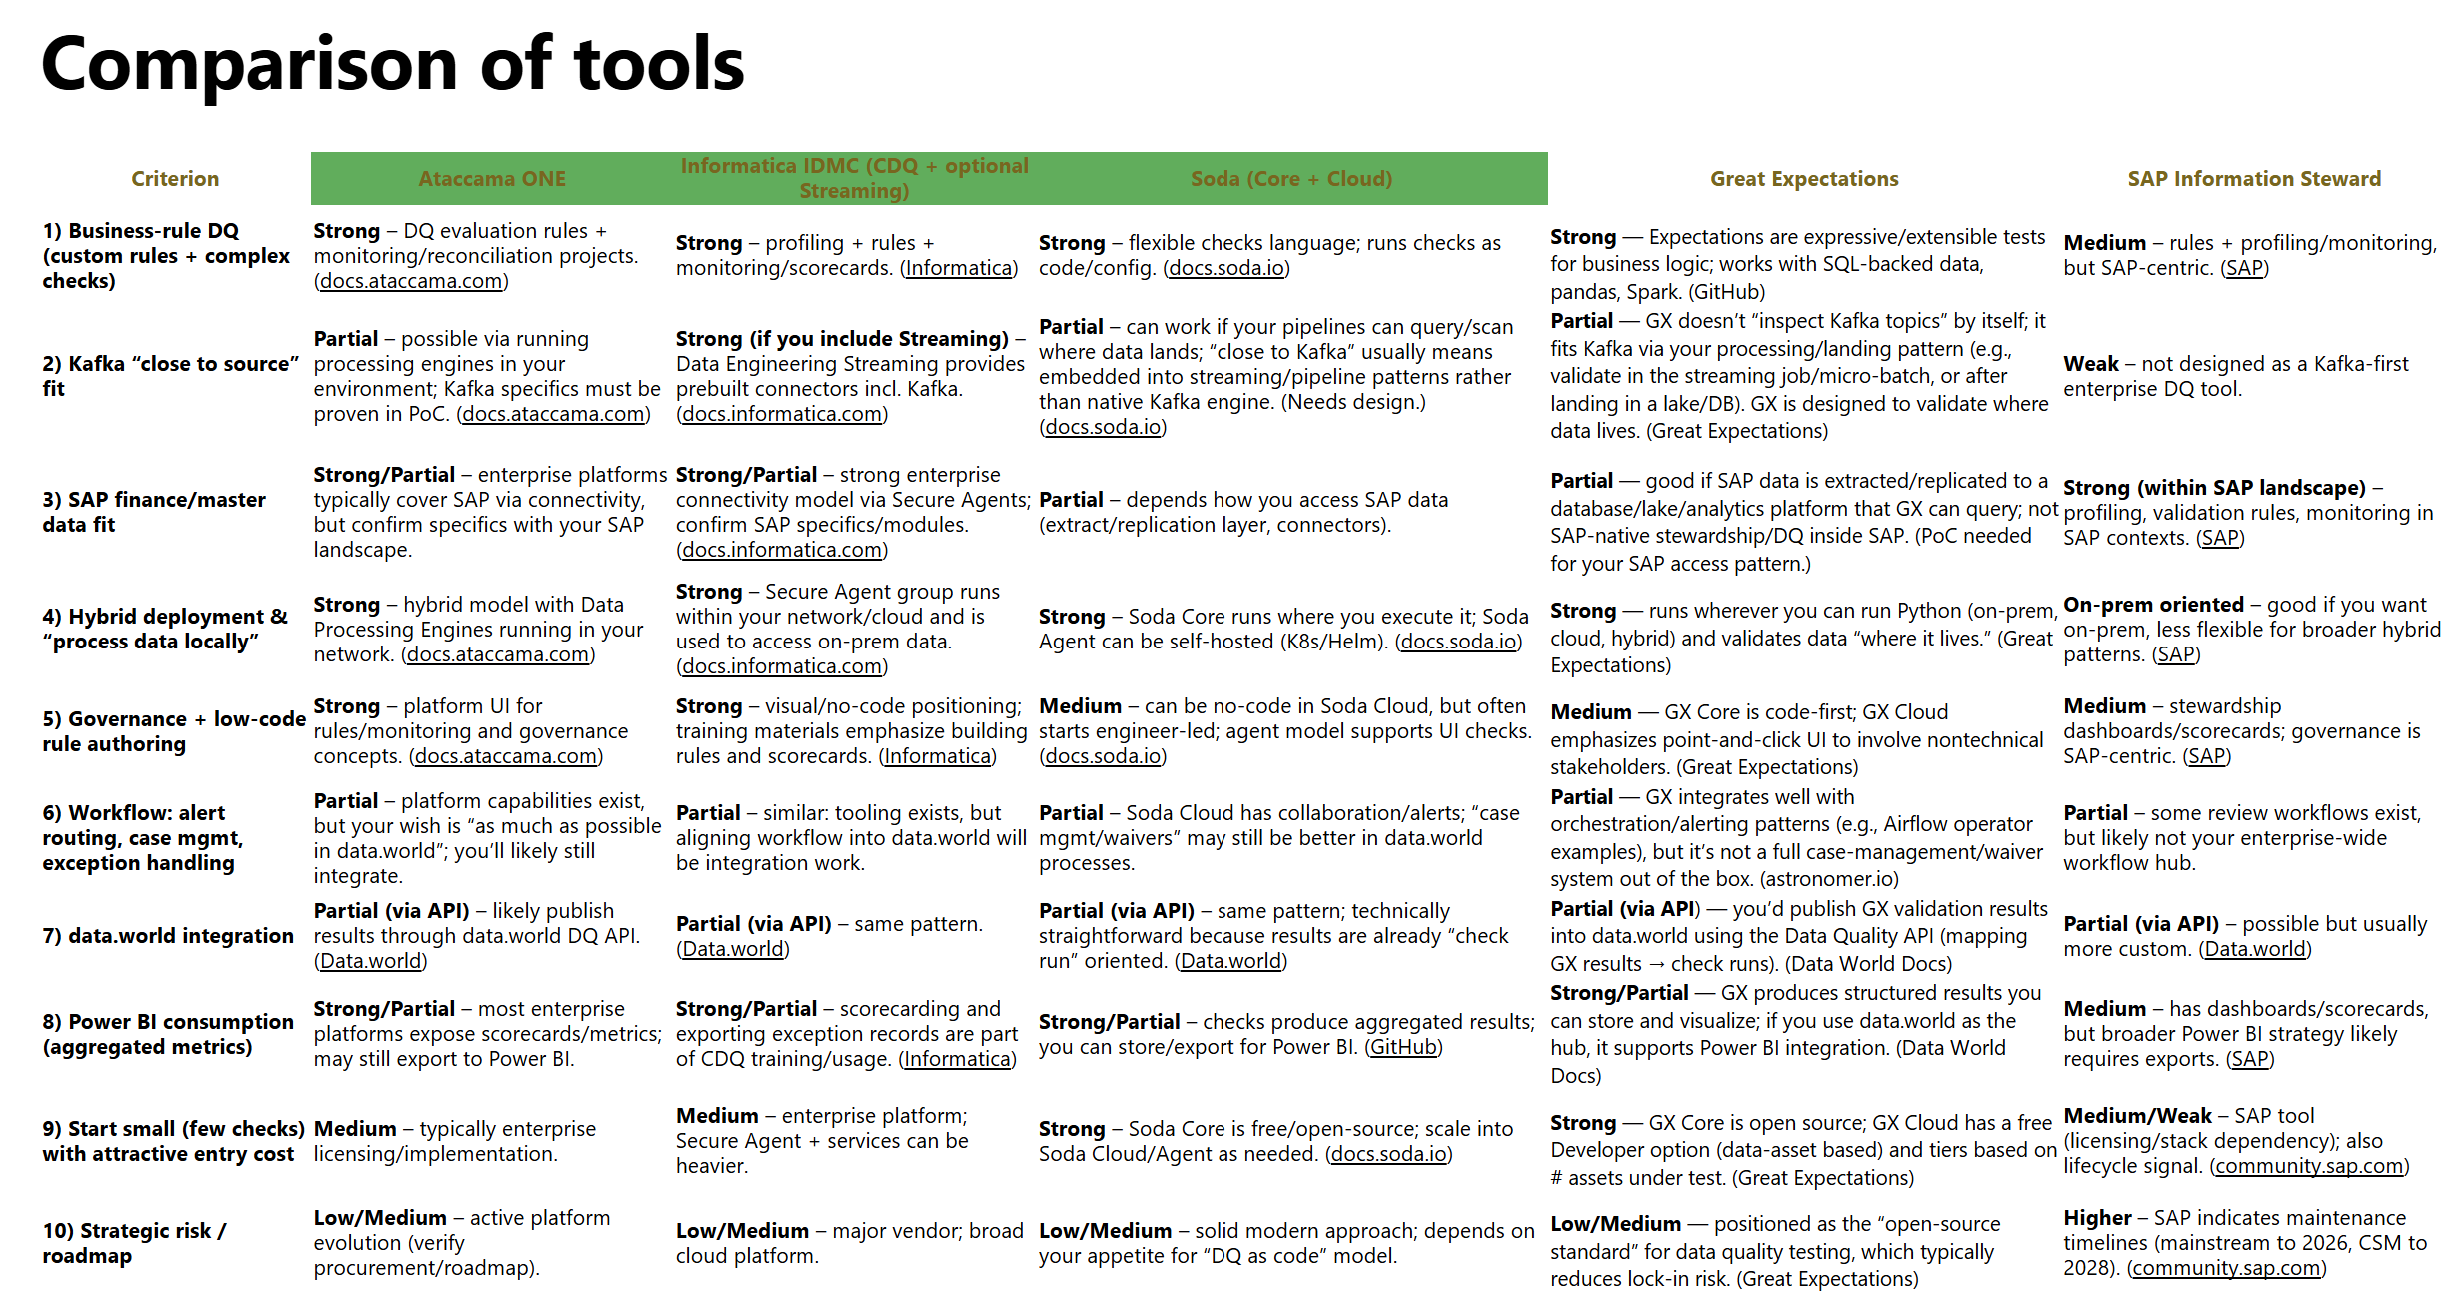
\includegraphics[width=0.95\textwidth]{./content/PostInput1/DQM_Tool_Evaluation_3.png}
    \caption{Example of the comparative evaluation matrix used during the assessment of different data quality management tools}
    \label{fig:dqm_tool_evaluation_3}
\end{figure}


\subsection*{Design decisions}
Next step after the evaluation table is to invite the succeeding tools to a demo. In this demo the providers are asked to show their performance of the tool against the defined criteria but can also show what specific benefit they bring with. The demo provides the selecting company with a more detailed view of the capabilities applied to their dataset or if any shortcommings are blocking the decision. Furthermore it allows the selecting company to directly ask questions on open items. After a demo the scoring can be adjusted and finally a decision made wether to go ahead with a provider into \gls{PoC} or even contract negotiations or send them the information that they dropped our of the selection.



\section{DQM tool testing}
Describes the testing of the tool...
what was required for an actual tool decision
What next follows
this is the basis for any work on the tool testing

\subsection*{Subsection No1}
This is the next subsection



\chapter{Implementation}
Todo
Write the implementation

This chapter uses the research findings and the solution landscape developed in the previous chapters as a basis for the implementation. With the defined SMART goals, the analysed reporting pipeline, and data lineage, this chapter provides step-by-step documentation leading to a rule-based data quality MVP within the DWH LS OPS. The re-engineering of the required data sources starts with the business description of the report usage, which ensures that the business key needs are mapped into the MVP. From the first section onward, the complex steps are presented to the reader in small, concise steps.

\chapter{Results}

This is the key chapter that reflects on the initial goals, the work carried out to achieve the goals, and the degree to which they were achieved. This chapter is structured around each goal, and special attention is paid to the key learnings that will be useful for subsequent phases of this work.


\section{Introduction}
The results presented here are part of a structured process that began step by step with the research question and led to the solution architecture and its implementation. Before delving further into the results of this project, a brief reminder of its scope helps to maintain focus. The project supports the \textbf{D}ata \textbf{W}are\textbf{h}ouse of \textbf{L}ogistic \textbf{S}ervices \textbf{Op}eration\textbf{s} (\gls{DWHLSOPS}) with the goal of improving \gls{DA} and \gls{DQ} management by replacing manual checks performed by the business with automated checks executed by IT. Through this change, data about these checks can become more consistent and enable the business to monitor them more easily. To achieve this, the existing reporting pipeline from raw data to the final report had to be re-engineered and documented.



\section{Evaluation criteria}
First, a result is defined as every piece of information that helps the reader become familiar with the context of the work. Second, it includes all information that supports understanding of the methods used during the project. Third, it comprises the main goal of this work, the SMART goals and their results. While the supporting results help to understand the environment, only the SMART goal results are the effectively relevant results of this work.

These SMART goals have been defined in the research chapter at \ref{ResearchSmartGoals}:

\begin{itemize}
\item \textbf{1) Setup of an improved data quality report}
\item \textbf{2) Evaluation and Selection of DQM platform for master thesis}
\item \textbf{3) Validatrion of selected DQM tool}
\end{itemize}



\section{SMART goal 1: Setup of an improved data quality report}
\subsection*{Goal definition}
\textbf{1) Setup of an improved data quality report}
    
\textbf{WHY:} This will help the team to run the daily checks faster

By the end of the implementation phase, the existing data quality report is to be updated to use the new infrastructure. This includes new reporting data pipelines and the new structure using star shema. Also, Power BI is to be used.

Success is measured by user feedback which has to be retrieved by \gls{ASTV} team. The feedback is to be implemented and the report must be on the productive systems.



\subsection*{Core results}
\begin{itemize}
    
\item \textbf{Update of data source:} In the implementation chapter, the data source for the third party checks was moved from beeing stored on a shared drive to beeing on sharepoint with a synchronisation onto \gls{AWSS3}. By this the data is versioned and available for other usage.

\item \textbf{Power BI Setup:} At the beginning of the implementation chapter, the setup of Power BI was performed. It used the existing guides of Swiss Post, and allowed in turn to start the development of the new improved \gls{DQM} report.

\item \textbf{Model data setup:} The data setup done trough out the course of the implementation chapters first section setup a model which was extentable. And allowed the usage of filters to be applied on all the data.

\item \textbf{New visuals to support faster interpretation by stakeholders:} The new visuals developed, allowed three things. The fast visual check if the data is correct on the four comparisions performed. They allow to see the changes on a timeline using the linechart and finally the table with the data allows the detailed check per day and location to be confirmed.

\item \textbf{Scrum review and after review feedback:} The scrum review showed the report to the whole \gls{ASTV} team and was a valuable means to get feedback. Further feedback was retrieved in separate meetings which was in turn applied. Resulting into the final version of the report beeing brought into production environment.

\item \textbf{New view Athena, and applied DevOps:} During the implementation of the report in Power BI, a separate view was setup in Athena. This new view allowed to use the new data sources while the old view was not touched and the two were not entangled. In addition for the deployment of this new view, the DevOps deployment process at Swiss Post was described and applied.
\end{itemize}




\subsection*{Supporting results}
The following results support the later implementation steps:
\begin{itemize}
    \item In the solution landscape chapter, the definition of Power BI as new reporting environment was established. Furthermore the change from wide table to star shema was established.

    \item In the solution architecture, the metrics are reflected in the definitions of the relevant submitted and discharged events, as described in Sections \ref{SolutionSubmittedEvent} and \ref{SolutionDischargedEvent}.
\end{itemize}

\subsection*{What was not achieved?}
All goals are fulfilled.

\subsection*{Goal verdict}
This goal was completely fulfilled. It has the report has been implemented including applying the feedback of the stakeholders.

\subsection*{Learning and outlook for future work}
In the importance of running checks between different environments from the first day of development. This is due to the issues that occured with the different environment of Power BI. Furthermore it's important to get the feedback of the stakeholders as soon as possible and plan enough time for the implementation of their requests.
\section{SMART goal 2: Investigation of IT systems for DQM metrics}
\subsection*{Goal definition}
\textbf{2) Investigation of IT systems for DQM metrics}

\textbf{WHY:} To define what DQM means in measurable terms.

By the end of the analysis phase, the IT systems and data stores are investigated, and it is defined where quality metrics can be implemented, stored, and evaluated within the DWH LS OPS environment.

Success is measured by a documented system overview that maps the selected metric to its technical source, storage location, and execution context. This is to be validated with IT stakeholders.


\subsection*{Core results}
This goal, while enriched with many supporting results, did not meet the core result of defining the storage and execution context. 
It is important to note that the rule-based DQM system was developed only as a proof of concept with a test case. Therefore, the position of the rule checks was not defined \ref{SolutionDQMEndOf2025}. This is, however, out of scope, as the rule check engine is developed by the DQM team working in parallel on this solution without involvement of the project team.


\subsection*{Supporting results}
\begin{itemize}
\item \textbf{Data lineage description:} The data lineage was described as follows: \textit{1) Physical data source:} Scans are performed on parcels by different scanners; \textit{2) Initial data storage:} The scan events are first saved in AWS S3; \textit{3) Kafka ingestion:} Apache Kafka ingests the events into a topic; \textit{4) Data delivery to DWH:} Apache Kafka is consumed by DWH LS OPS, where the data is saved to the raw layer. This is described in Section \ref{SolutionDataLineage}.

\item \textbf{Reporting pipeline description:} The reporting pipeline of DWH LS OPS is defined as follows: the \textbf{storage layer} using Amazon S3, followed by the \textbf{query and processing layer} using Amazon Athena and SAP Datasphere (DSP), and finally the \textbf{consumption layer} using SAP Analytics Cloud (SAC). These steps are detailed in Section \ref{SolutionReportingPipeline}.

\item \textbf{Placement of data quality checks:} Data quality checks are most effectively placed on the processing and transformation layer. This allows both meaningful and effective validation. Earlier checks on the data lineage and reporting pipeline are limited to global completeness, while later checks on the reporting layer are too late to enable corrective action. This is discussed in Section \ref{ResearchDataQChecksOnDataLifecycle}.

\item \textbf{Results of DQM checks:} The DQM team defined that the results of rule checks are to be stored in a rule-check database. However, this solution was not yet installed in DWH LS OPS at the time of this analysis. This is described in Section \ref{SolutionDQMTeamHighLevelTarget}.
\end{itemize}


\subsection*{What was not achieved?}

\begin{itemize}
    
\item \textbf{IT stakeholder confirmation:} Formal confirmation of the data lineage and the reporting pipeline was not obtained from IT stakeholders.

\item \textbf{DQM check storage location:} The location where DQM check results are to be stored was not defined.

\end{itemize}


\subsection*{Goal verdict}
This SMART goal was \textbf{partially achieved}, as two targets were not met.

\textbf{Why:} First, the DQM check storage location was not defined; however, this is out of scope because responsibility for the application lies with the DQM team. Second, formal confirmation with IT stakeholders regarding the data lineage and reporting pipeline was not conducted.


\subsection*{Learning and outlook for future work}
Regarding the missing alignment with IT stakeholders, the data lineage was initially considered general knowledge within the team and therefore not documented first. Once it was available, discussion with IT stakeholders was no longer possible due to time constraints. Second, the position for saving DQM results was out of scope.

For the first point, aspects that appear obvious should be documented earlier when confirmation is required. Regarding out-of-scope topics, communication with external teams needs to be more proactive in order to identify earlier when deliverables are delayed or when priorities change.
\section{SMART goal 3: Investigation of data lineage for metrics}
\subsection*{Goal definition}
\textbf{3) Investigation of data lineage for metrics}

\textbf{WHY:} To apply DQM checks to the correct data sources and enable root cause analysis.

By the end of the analysis phase, investigate and document the data lineage from data ingestion to the reporting layer.

Success is measured by a documented lineage description that allows data to be followed through the system and its transformations to be understood, including the validation possibilities available to responsible stakeholders.



\subsection*{Core results}
\begin{itemize}
    
\item \textbf{Business report documentation:} The business report for message processing DQM was documented. The key information was identified as \textbf{Diff\_Discharged\_Submitted}. Both submitted and discharged values should be in the same number range, as this check serves to ensure data completeness. This is because every mail piece in a sorting center has one submitted and one discharged event count per day, as the machines are empty at the end of every day. Therefore, the difference between these values needs to be below the threshold of 0.01. This is described in section \ref{Implementation1SubmittedDischargedDifference}.

\item \textbf{Key value identification:} In the implementation chapter, the quality metrics of submitted and discharged, in conjunction with the difference between the two (\textbf{Diff\_Discharged\_Submitted}), were identified. These metrics represent the key values used to evaluate the daily completeness of data (Section \ref{Implementation1SubmittedDischargedDifference}).

\item \textbf{SAC report documentation:} The report information relevant to the MVP was identified, including the date, three-letter location key, submitted number, discharged number, and their ratio, and was documented in section \ref{sectionSVADQMReport}.

\item \textbf{DSP data model description:} Within the DSP, the data lineage of the entire report was examined. A key finding was the location where the ratio is calculated, namely within the DSP data model. Furthermore, it was identified that the data for the MVP case is based solely on AWS Athena; see section \ref{ImplementationInvestigateDSP}.

\item \textbf{Business stakeholder confirmation:} The AWS Athena query was traced, and during a meeting with the stakeholders, the key information was confirmed. This is described in section \ref{ImplementationFourBusinessMeeting}.

\item \textbf{AWS Athena query:} A concise analysis of the query structure and the AWS Athena–specific SQL was conducted, identifying the first relevant components. Finally, documentation was created and presented to the DQM team, as described in section \ref{subsectionAthenaQuery}.

\item \textbf{DQM team update:} To update the DQM team, the data lineage from the AWS Athena query, including relevant accounts, was documented. This includes a brief introduction to the use case and the query for the MVP in section \ref{ImplementationFourConfluenceDocu}. The meeting is documented in appendix \ref{apendixDQM1911}.

\end{itemize}

\subsection*{Supporting results}

\begin{itemize}
\item \textbf{Data lineage description:} The data lineage was described from: \textit{1) the physical data source:} scans are performed on parcels by different scanners, \textit{2) the initial data storage:} the scan events are first saved in AWS S3, \textit{3) Kafka ingestion:} Apache Kafka ingests the events into a topic, \textit{4) data delivery to DWH:} Apache Kafka is consumed by DWH LS OPS, where the data is saved to the raw layer. This is described in Section \ref{SolutionDataLineage}.

\item \textbf{Reporting pipeline description:} The reporting pipeline of DWH LS OPS is defined as the \textbf{storage layer} using Amazon S3, followed by the \textbf{query and processing layer} using Amazon Athena and SAP Datasphere (DSP), and finally the \textbf{consumption layer} using SAP Analytics Cloud (SAC). These steps are detailed in Section \ref{SolutionReportingPipeline}.

\item \textbf{Placement of data quality:} Data quality checks are best placed on the processing and transformation layer. This allows both meaningful and effective tests. Earlier checks on the data lineage and reporting pipeline are less effective, as only global data completeness can be verified, while later checks on the reporting layer remove the possibility of corrective action. This is described in Section \ref{ResearchDataQChecksOnDataLifecycle}.

\item \textbf{Key value identification:} In the implementation chapter, the quality metrics of submitted and discharged events, in conjunction with the difference between the two (\textbf{Diff\_Discharged\_Submitted}), are identified. These metrics represent the key values used to evaluate the daily completeness of data (Section \ref{Implementation1SubmittedDischargedDifference}).
\end{itemize}

\subsection*{What was not achieved?}

The goal was completely fulfilled; nothing was left unachieved.


\subsection*{Goal verdict}
This goal was completely fulfilled. All required deliverables have been provided for this SMART goal.
These include:
\begin{multicols}{2}
\begin{itemize}
    \item \textbf{Supporting} Data lineage description
    \item \textbf{Supporting} Reporting pipeline description
    \item \textbf{Supporting} Placement of data quality
    \item \textbf{Supporting} Key value identification    
    \item \textbf{Core} Business report documentation
    \item \textbf{Core} Key value identification
    \item \textbf{Core} SAC report documentation
    \item \textbf{Core} DSP data model description
    \item \textbf{Core} Business stakeholder confirmation
    \item \textbf{Core} AWS Athena query 
    \item \textbf{Core} DQM team update
\end{itemize}
\end{multicols}


\subsection*{Learning and outlook for future work}

This allowed the identification of the key measurements for DQM. As this SMART goal was fully successful, no further learnings are carried forward to subsequent projects, aside from the tools SAC and DSP, which were examined in detail during their fulfillment.



\section{Summary}
With this chapter, the SMART goals defined in the research chapter have been analysed for completion. Two goals were completely fulfilled, one partially. The partially fulfilled second goal was limited due to responsibility constraints related to personal and team responsibility. The goal with partial fulfilled results points towards the need for goals planed along the lines of responisbilities, in addition to realistic time frames. However, it is important to note that even tough one goal was not reached completely, the overall results of the research helped to provide a solid for subsequent master thesis.



\chapter{Reflection and outlook}

The reflection chapter concludes the second steps in the epic quest of the academic team towards the improvement of data quality and data availability at Swiss Post. It evaluates the project with regard to methodology, content, and personal learnings, and then concludes with an outlook on how the project may be followed up.

\begin{figure}[H]
    \centering
    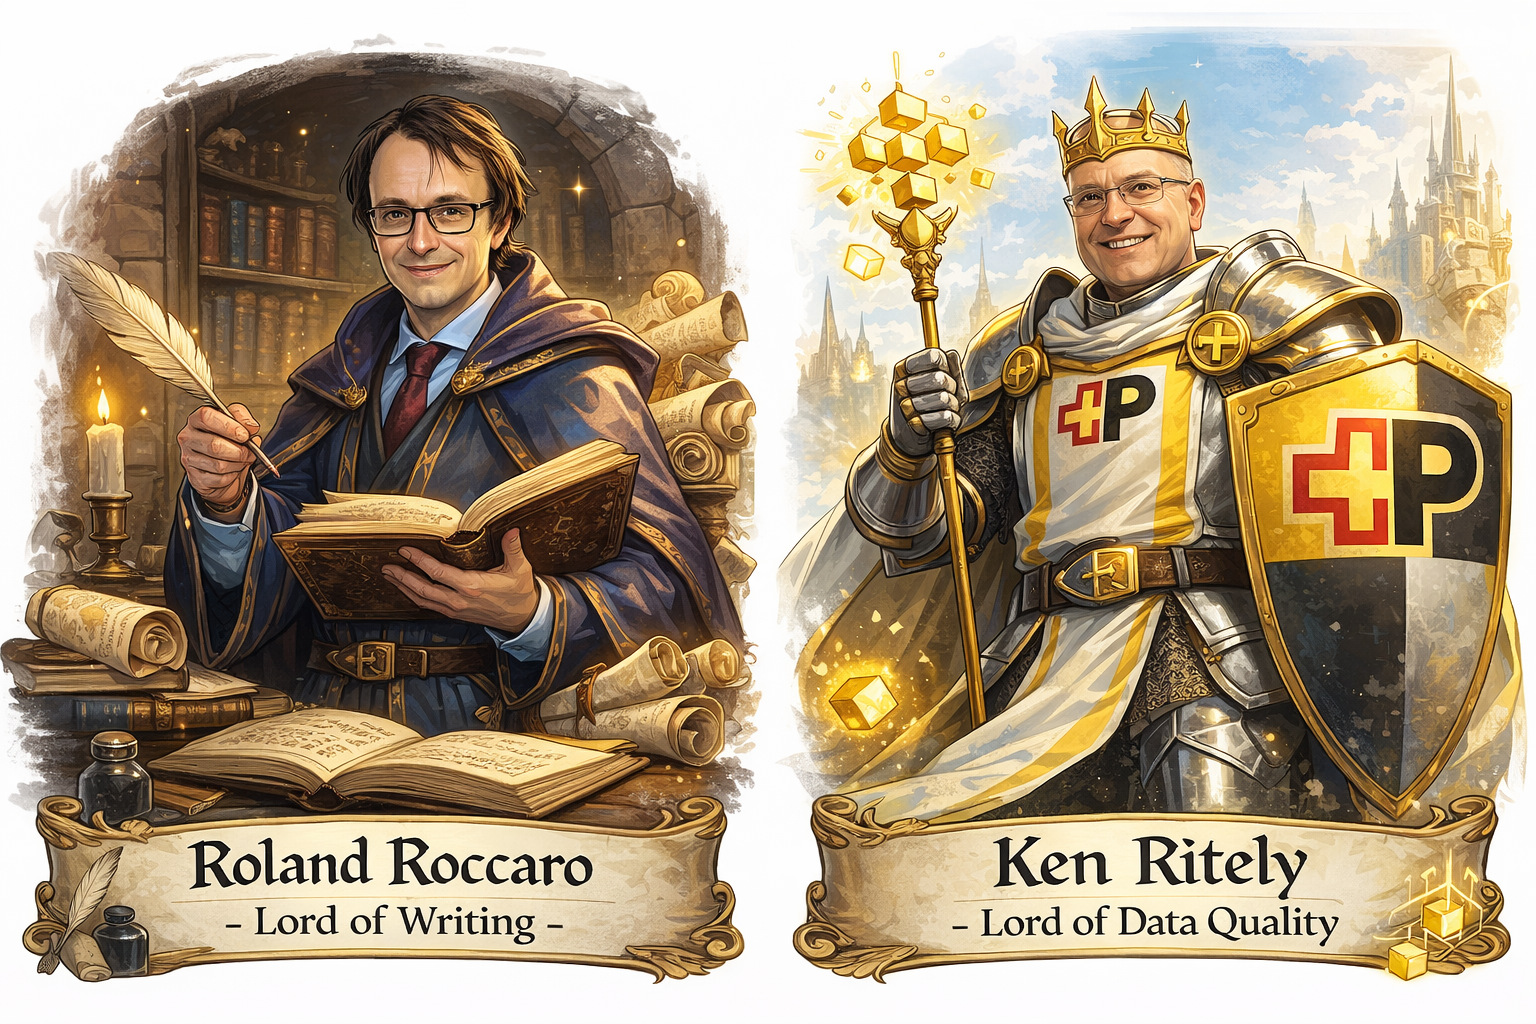
\includegraphics[width=0.8\textwidth]{./content/img/ProjectManagement/LordsOfDQM.png}
    \caption{Reflections with the lords of DQM}
    \label{fig:reflection_lords_of_dqm}
\end{figure}



\section{Methodological Reflection}
In this section, the methodology is reflected. This is not limited to the project management methodology but looks overall at all methods applied.

\subsection*{What went well}
The following list of items went well, including a reasoning why they went well.

\begin{itemize}
    \item \textbf{Documentation using Miro}: The documentation of the project on Miro went well. The tool proved very useful for fast notes, which were brought into the document later. It was also used for project management and is a key information resource for the entire project.
    \item \textbf{Weekly meetings, Jour Fixe}: The Jour Fixe, as documented in Miro, was held weekly. It proved to be a valuable exchange and helped guide the work and larger tasks. Its documentation on paper was uploaded to Miro, which helped in keeping track of discussed and important decisions.
    \item \textbf{Weekly meeting structure}: The meeting structure, starting with an introduction to the topic, the deliverables worked on, and a milestone status update, helped to structure the meetings and eased the start into another session after one week. Furthermore, the predefined questions helped to keep the discussion focused on the important topics. The deliverables graphic, together with the broad description of discharged and submitted items on Miro, supported this.
    \item \textbf{Milestone structuring}: The milestones helped to keep the time effort per chapter structured. They helped to stop basic research at the right moment and to move towards the solution landscape and implementation.
    \item \textbf{Writing mode}: The writing mode, with corrections using ChatGPT based on a defined prompt, went well after it was defined. It helped to iron out earlier occurrences of non-academic writing and grammatical issues.
    \item \textbf{Kanban}: The Kanban board helped to keep track of tasks. While the usage can still be improved, noting important decisions as tasks helped to keep track of them.
\end{itemize}


\subsection*{What did not go well}

\begin{itemize}
    \item \textbf{Work on every Friday and Wednesday afternoon}: According to planning at the start of the project, the full friday with approximately eight hours and the wednesday afternoon with aproximately 4 hours at work were reserved for work on the projet. This was not always possible as the timetracking for work shows. This was compensated with working on other days then planned. However time blockers will need to be re-negotiated for the next project.
    \item \textbf{Split between work at Swiss Post and academic work}: The 50\% to 50\% split between both engagements was not possible. At the beginning of the project, a delayed work project consumed all efforts and blocked from an early start into the project tasks, while later interruptions on production systems had to be fixed imediately rather than on the next day. This affected the start of the academic project which was postponed till early October which affected the scope.
    \item \textbf{Writing speed}: The writing speed proofed to be lower than expected. Instead of reaching a first draft before Xmas holidays, the first complete draft was only available early january. This showed the need for an earlier start with more writing. 
    \item \textbf{Rewriting of chapters}: Some chapters such as the results chapter were written in a first draft which had to be completely rewritten. This was a learning regarding required academic writing structure. In the following projects, this will be known an can be evaded.
\end{itemize}



\section{Content-related Learnings}
% Was habe ich über DQM, DA, Lineage, Organisation gelernt?

\begin{itemize}
    \item \textbf{Data lineage and reporting pipeline}: The complex data lineage at Swiss Post, including the path from physical sensors through Apache Kafka to Amazon S3 storage. The number of steps until the data is available as a report is higher than expected. Even before the data is stored in the cloud in a raw state, it has already passed through at least three processing steps. Adding the reporting pipeline further increases the complexity, which at this stage is at least partly the responsibility of the reporting team.
    \item \textbf{Where to check data quality and availability}: Data quality and availability checks need to be set up at different positions within the data lineage and reporting pipeline. While data availability is best checked early, data quality can only be checked in later stages when the data is joined with organisational information. For example, checking whether a postal code is valid requires a join with a postal code register when not only the number of digits but whether the code exists should be verified.
    \item \textbf{Independence of data quality and availability}: Data can be available but incorrect, or unavailable but correct. This is because availability can be time-based. For example, data needs to be available at 07:00; if it is not available at 07:00 but arrives at 07:02 and is correct, the data was simultaneously unavailable while its quality was acceptable.
    \item \textbf{Technical documentation requirements}: When setting up the documentation for the DQM team, it became apparent which information is important, such as missing account information in the first version. Documentation within the same team often does not require such details, but communication with another team requires this key information, including more guidance on how to navigate an unfamiliar environment, such as the different databases in Amazon Athena.
    \item \textbf{Use case feasibility}: The research and documentation of existing checks performed by the business showed that they can be replaced with automated rule-based checks. Furthermore, the implementation demonstrated the steps required to set up the rules for future DQM checks.
    \item \textbf{Tool-related}: During the work, many new tools were explored, such as DSP with its data lineage capabilities. This enabled the acquisition of new knowledge that is useful for future work.
    \item \textbf{Language-related}: The analysis of the query structure used in the DQM view helped to understand Amazon Athena–specific structures and also deepened knowledge of CTE usage in three-layered aggregations.
    \item \textbf{Usefulness of heterogeneity}: While the heterogeneity of Swiss Post poses challenges at the reporting level, it is essential at the operational and risk management levels. For example, managing plants of different sizes in the same way would create management overhead, and relying on a single hardware provider would introduce significant risks.
    \item \textbf{IT complexity}: Swiss Post has a large IT infrastructure that is managed by multiple teams working together towards the common goal of keeping systems running and improving them. This creates constraints, as multiple teams work on shared initiatives. While this can be beneficial, as not everything needs to be handled by a single team, it also requires coordination of solutions and architectures, often shifting new implementations from greenfield to brownfield environments.
\end{itemize}



\section{Personal Learnings \& Outlook}

In the course of this work, the author has learned many things; the following list summarises the most important learnings and their expected impact on future work.

\begin{itemize}
    \item \textbf{Importance of better planning}: Instead of assuming that something may be done in two or three days, the amount of learning required for unknown tools must be considered. Tasks should therefore be evaluated with regard to the tooling required. If the tooling is unknown, the learning time should be added to the time required for the task.
    \item \textbf{Organisational constraints}: Due to the size of Swiss Post, many activities happen in parallel. Multiple teams can work on the same initiatives, but often on different aspects. Identifying these activities prior to starting can help to avoid duplicated research. This, however, requires more preparation time and management, as well as communication within the organisation.
    \item \textbf{Research the obvious earlier}: For example, the DQM team did have some documentation, but this documentation was not sufficient for the rule-based DQM initiative. Reviewing this information in more detail earlier in the project would lead to a better understanding of the initial situation.
    \item \textbf{Communication with external teams}: External teams have different delivery goals and timelines. To avoid incorrect assumptions about their deliverables, these plans need to be tracked explicitly. This requires earlier communication and research into their timelines and delivery goals. Based on this information, the planning of the project team can be adapted.
    \item \textbf{Start the writing earlier}: The writing process was started early with the first chapters; however, the bulk of the writing was completed after the implementation. Starting the writing process earlier would shift research activities that occur during writing to an earlier stage. Having the chapters on which the implementation is based available earlier also allows the work to be structured more effectively.
    \item \textbf{Focus on what is relevant}: When taking screenshots, it is not necessary to capture the entire screen. It is more important to highlight the relevant information rather than documenting where in the tool the information can be found. Using lenses or smaller screenshots is therefore identified as a learning and goal for the next project.
\end{itemize}




\section{General setup, next steps}
\section{Todo, rewrite this... taken from Reseach Chapter}
As stated earlier the solutional goal of this project and its follow up is to provide an MVP for DQM, from
which the key learnings will enable the full “future state” reporting solution. This MVP should implement
anautomaticdataqualitycheck,replacinganoccasional,nonautomatedcheckperformedbythebusiness.
This is important, as the DQM check is currently executed by the business instead of IT, which creates
challenges with regard to the desired target state. The expected situation would be that IT executes data
quality checks and de nes thresholds together with the business. At present, however, the knowledge
about thresholds and other relevant information resides solely with the business.
Insummary,havingITrunthedatacheckswouldenablecontinuousfollow-upofdataquality. Forexample,
a report based on automatically executed checks could show system uptime over a longer period of time.
This information would later allow IT to extrapolate standard value ranges, which in turn would enable
the de nition of alerting thresholds. In short, having DQM checks executed automatically rather than
occasionally by the business provides multiple bene ts for both IT and the business

Here... the planning of the master thesis was a big part of all the follow up work

\begin{figure}[H]
    \centering
    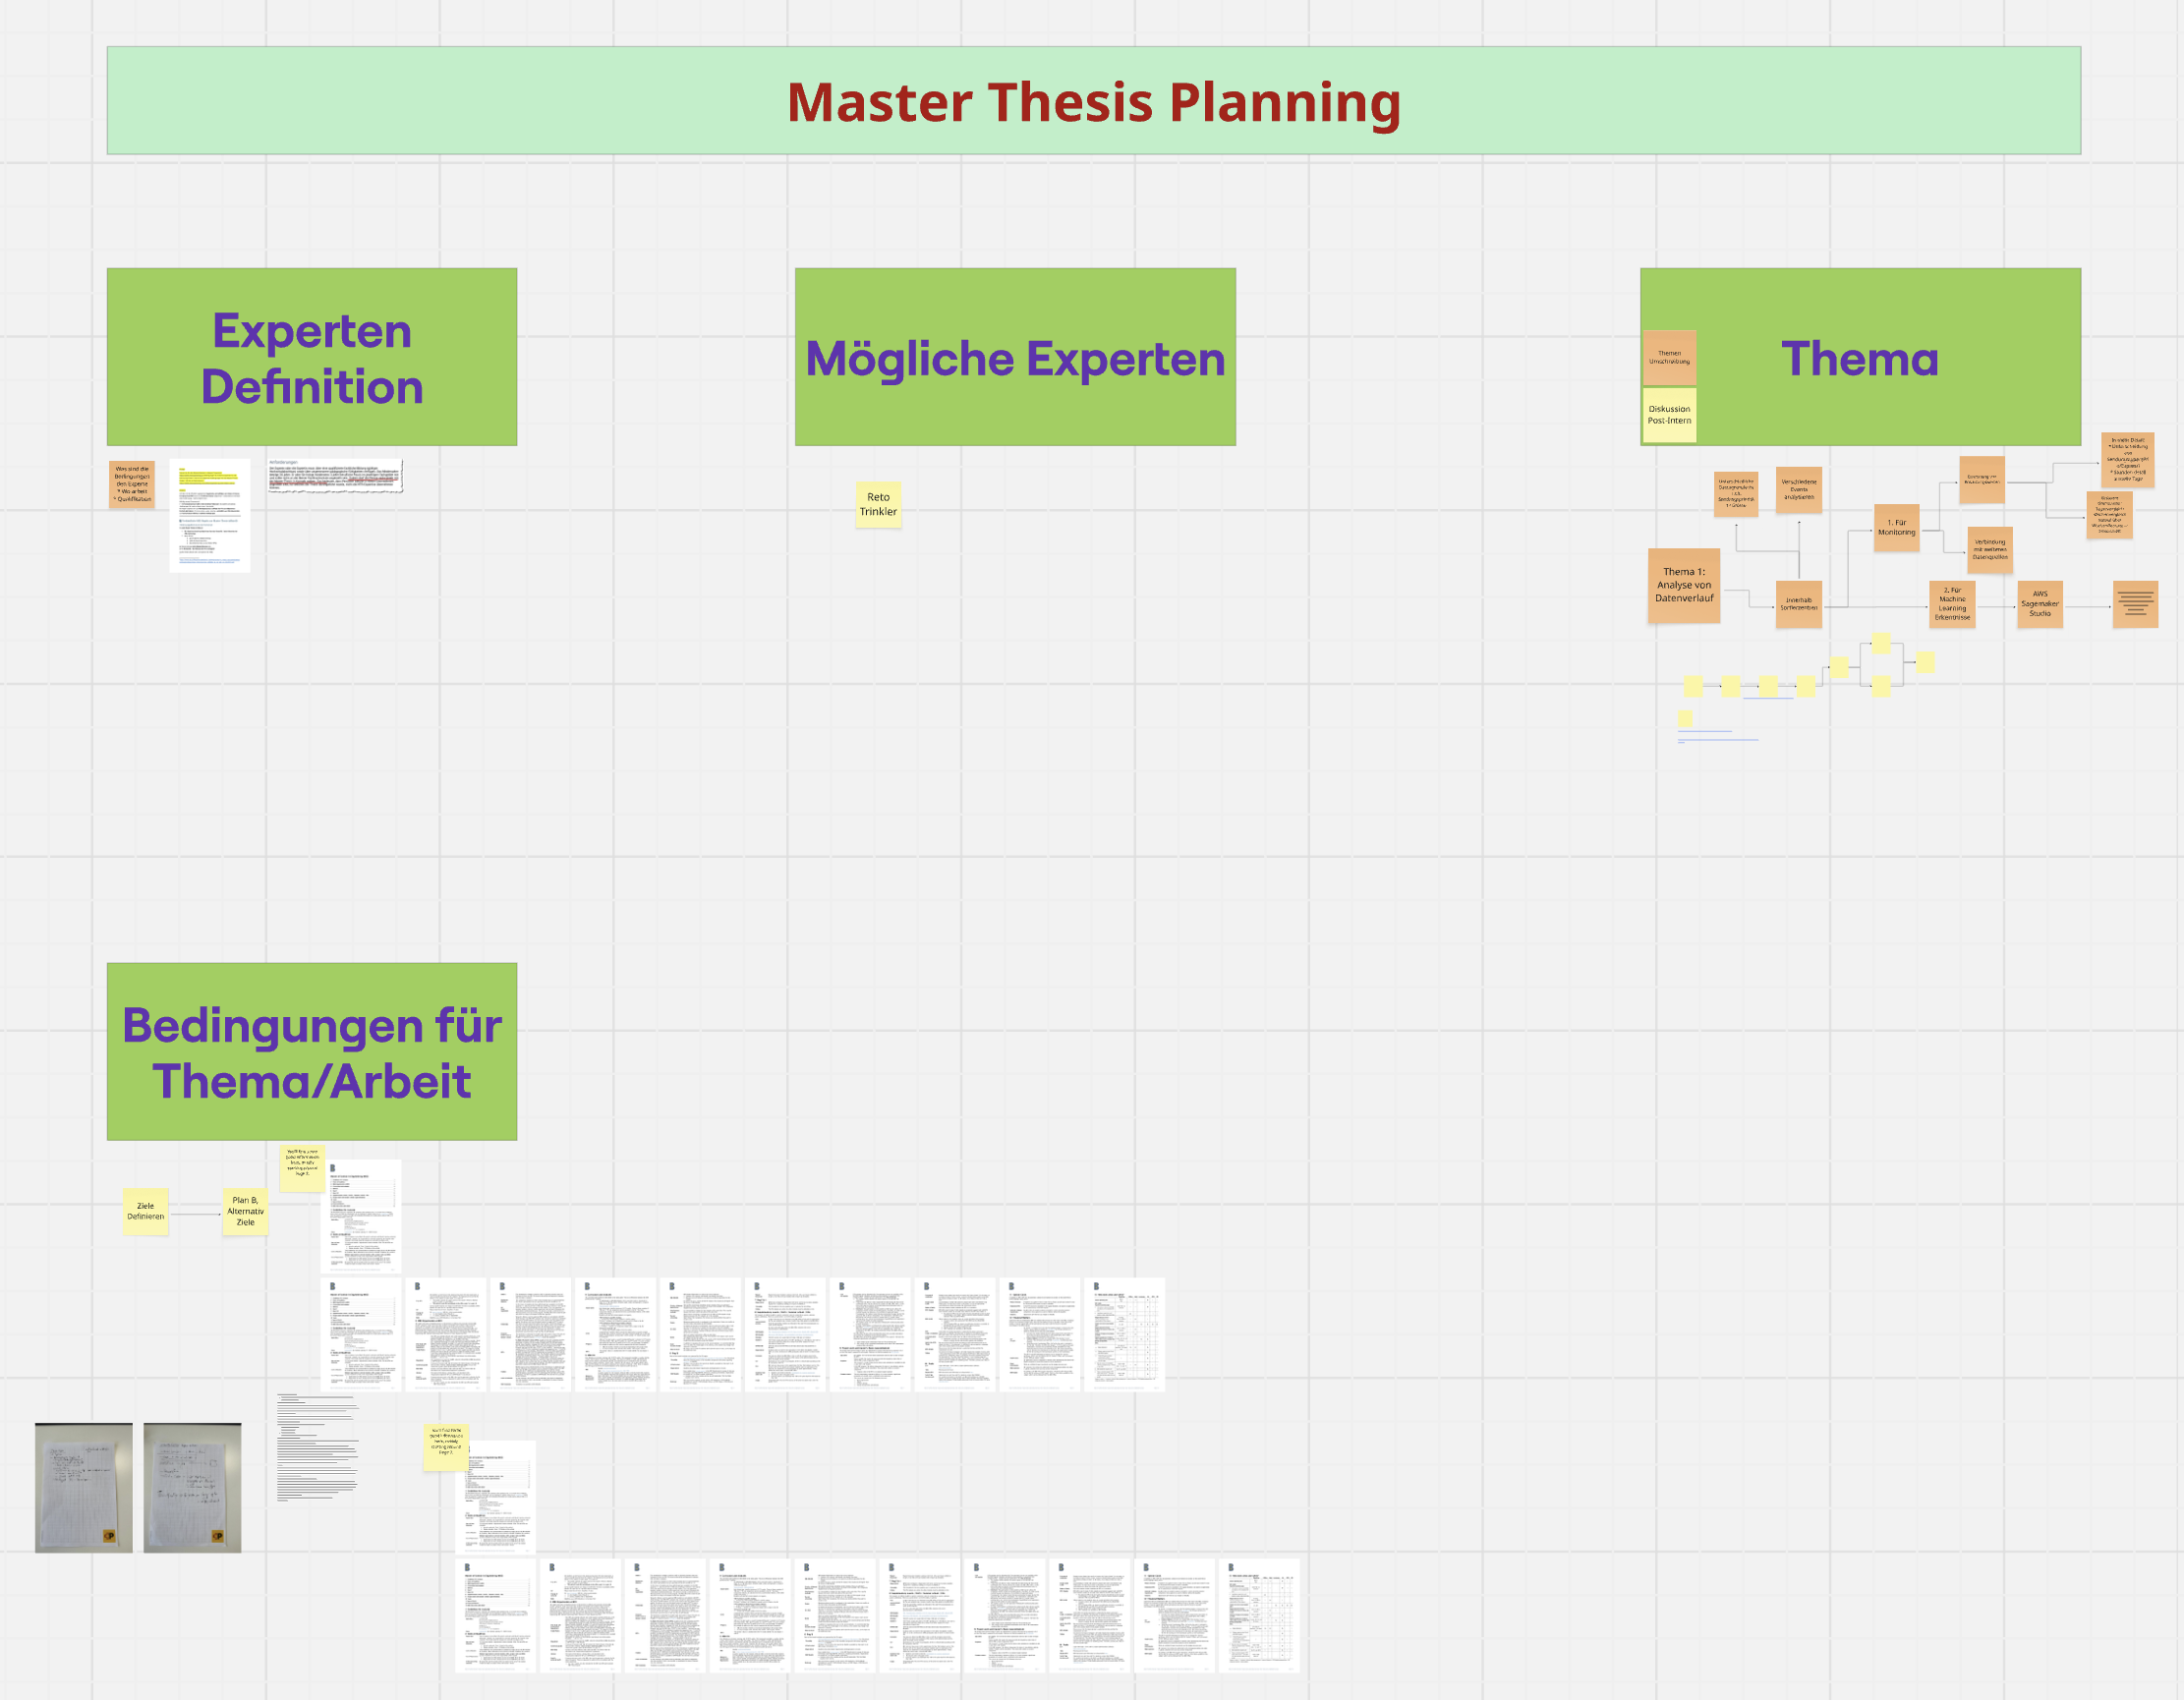
\includegraphics[width=\textwidth]{./content/img/MiroBoard_MasterThesis_Planning.png}
    \caption{Extract of the Miro board illustrating the planning of the subsequent master's thesis. The section documents initial ideas, work packages, dependencies and planning considerations that emerged during Project~2 and served as preparation for the continuation of the research.}
    \label{fig:annex_miro_masterthesis}
\end{figure}
\chapter{Statement of Authorship}
The author hereby declares that this work is the result of their own independent effort and that no sources other than those listed in the bibliography and identified as references have been used.  
Glossary entries have been partially written by the author using public descriptions (e.g., product homepages), copied from Wikipedia, or generated by ChatGPT based on provided bullet points. Further details regarding the use of LLM is decribed within the project management chapter.

\listoffigures
\listoftables
\addcontentsline{toc}{chapter}{Glossary}
\printglossary[title={Glossary}]

\printbibliography


\appendix
\chapter{Amazon Athena Queries}

This appendix provides the Amazon Athena queries. They are stored here since putting them into the document would disrupt normal flow.

\section{Full DQM view query}
\label{fullDQMquery}
The full query which creates the view beeing main data source of the DQM report.

\begin{lstlisting}[style=sqlstyle]
CREATE OR REPLACE VIEW "sendungsverarbeitung_dqm_v" AS
WITH
key_to_plz AS (
    SELECT 'VET' AS locationKey, '196000' AS plz
    UNION ALL SELECT 'HRK', '462150'
    UNION ALL SELECT 'CAD', '659100'
    UNION ALL SELECT 'WAL', '830000'
    UNION ALL SELECT 'HAE', '462000'
    UNION ALL SELECT 'UTZ', '720000'
    UNION ALL SELECT 'PRA', '413400'
    UNION ALL SELECT 'FRA', '852000'
    UNION ALL SELECT 'DAI', '131000'
    UNION ALL SELECT 'URD', '892000'
    UNION ALL SELECT 'BCH', '503000'
    UNION ALL SELECT 'RUE', '815000'
    UNION ALL SELECT 'OMU', '307100'
),

plz_to_key AS (
    SELECT '196000' AS plz, 'VET' AS locationKey
    UNION ALL SELECT '462150', 'HRK'
    UNION ALL SELECT '659100', 'CAD'
    UNION ALL SELECT '830470', 'WAL'
    UNION ALL SELECT '830000', 'WAL'
    UNION ALL SELECT '462000', 'HAE'
    UNION ALL SELECT '720000', 'UTZ'
    UNION ALL SELECT '413400', 'PRA'
    UNION ALL SELECT '852000', 'FRA'
    UNION ALL SELECT '131000', 'DAI'
    UNION ALL SELECT '892000', 'URD'
    UNION ALL SELECT '503000', 'BCH'
    UNION ALL SELECT '815000', 'RUE'
    UNION ALL SELECT '307100', 'OMU'
),

mp_discharged_raw AS (
    SELECT
        CAST(
            DATE_ADD(
                'hour', -6,
                discharged.timestamp AT TIME ZONE 'Europe/Zurich'
            ) AS DATE
        ) AS Posttag,
        discharged.sortingunit.locationKey AS locationKey,
        discharged.sourceId AS sourceId
    FROM curated_lsops.mailpiece_discharged
),

mp_discharged AS (
    SELECT
        Posttag,
        locationKey,
        CASE
            WHEN locationKey IN ('CAD','HRK','PRA','UTZ','VET','WAL')
                 AND sourceId NOT LIKE 'w%'
                 AND sourceId NOT LIKE 'W%'
                 AND TRIM(sourceId) <> '' THEN 1
            WHEN locationKey IN ('BCH','RUE','OMU') THEN 1
            WHEN locationKey IN ('HAE','FRA','DAI','URD') THEN 1
            ELSE 0
        END AS relevant_discharged
    FROM mp_discharged_raw
),

discharged_agg AS (
    SELECT
        Posttag,
        locationKey,
        SUM(relevant_discharged) AS num_discharged
    FROM mp_discharged
    GROUP BY 1, 2
),

mp_submitted_raw AS (
    SELECT
        CAST(
            DATE_ADD(
                'hour', -6,
                submitted.timestamp AT TIME ZONE 'Europe/Zurich'
            ) AS DATE
        ) AS Posttag,
        submitted.sortingunit.locationKey AS locationKey,
        submitted.sortingProcess AS sortingProcess
    FROM curated_lsops.mailpiece_submitted
),

mp_submitted AS (
    SELECT
        Posttag,
        locationKey,
        CASE
            WHEN locationKey IN ('HRK','VET','CAD','WAL','UTZ','PRA')
                 AND sortingProcess = 'AUTOMATIC' THEN 1
            WHEN locationKey IN ('BCH','RUE','OMU') THEN 1
            WHEN locationKey IN ('HAE','FRA','DAI','URD') THEN 1
            ELSE 0
        END AS relevant_submitted
    FROM mp_submitted_raw
),

submitted_agg AS (
    SELECT
        Posttag,
        locationKey,
        SUM(relevant_submitted) AS num_submitted
    FROM mp_submitted
    GROUP BY 1, 2
),


mp_coded_raw AS (
    SELECT
        coded.sortingCycleId AS sortingCycleId,
        CAST(
            DATE_ADD(
                'hour', -6,
                coded.timestamp AT TIME ZONE 'Europe/Zurich'
            ) AS DATE
        ) AS Posttag,
        coded.sortingunit.locationKey AS locationKey,
        coded.sortingProcess AS sortingProcess
    FROM curated_lsops.mailpiece_coded
),

mp_coded AS (
    SELECT DISTINCT
        sortingCycleId,
        Posttag,
        locationKey,
        CASE
            WHEN locationKey IN ('HRK','VET','CAD','WAL','UTZ','PRA')
                 AND sortingProcess = 'AUTOMATIC' THEN 1
            WHEN locationKey IN ('BCH','RUE','OMU') THEN 1
            WHEN locationKey IN ('HAE','FRA','DAI','URD') THEN 1
            ELSE 0
        END AS relevant_coded
    FROM mp_coded_raw
),

coded_agg AS (
    SELECT
        Posttag,
        locationKey,
        SUM(relevant_coded) AS num_coded
    FROM mp_coded
    GROUP BY 1, 2
),

mp_destinationAssigned_raw AS (
    SELECT
        destinationAssigned.sortingCycleId AS sortingCycleId,
        CAST(
            DATE_ADD(
                'hour', -6,
                destinationAssigned.timestamp AT TIME ZONE 'Europe/Zurich'
            ) AS DATE
        ) AS Posttag,
        destinationAssigned.sortingunit.locationKey AS locationKey,
        destinationAssigned.sortingParameters.sortingProcess AS sortingProcess
    FROM curated_lsops.mailpiece_destinationassigned
),

mp_destinationAssigned AS (
    SELECT DISTINCT
        sortingCycleId,
        Posttag,
        locationKey,
        CASE
            WHEN locationKey IN ('HRK','VET','CAD','WAL','UTZ','PRA')
                 AND sortingProcess = 'AUTOMATIC' THEN 1
            WHEN locationKey IN ('BCH','RUE','OMU') THEN 1
            WHEN locationKey IN ('HAE','FRA','DAI','URD') THEN 1
            ELSE 0
        END AS relevant_destinationAssigned
    FROM mp_destinationAssigned_raw
),

destinationassigned_agg AS (
    SELECT
        Posttag,
        locationKey,
        SUM(relevant_destinationAssigned) AS num_destinationassigned
    FROM mp_destinationAssigned
    GROUP BY 1, 2
),

sendungsverarbeitung_raw AS (
    SELECT
        sva.datum_sort.datum AS Posttag,
        plz_to_key.locationKey AS locationKey,
        sva.sortierung.sortierprozess_typ AS sortierprozess_typ
    FROM infoblock_lsops.sendungsverarbeitung sva
    LEFT JOIN plz_to_key
        ON plz_to_key.plz = sva.zentrum.zentrum_plz
),

sendungsverarbeitung AS (
    SELECT
        Posttag,
        locationKey,
        CASE
            WHEN locationKey IN ('HRK','VET','CAD','WAL','UTZ','PRA')
                 AND sortierprozess_typ = 'AUTOMATIC' THEN 1
            WHEN locationKey IN ('BCH','RUE','OMU') THEN 1
            WHEN locationKey IN ('HAE','FRA','DAI','URD') THEN 1
            ELSE 0
        END AS relevant_sva
    FROM sendungsverarbeitung_raw
),

sva_agg AS (
    SELECT
        Posttag,
        locationKey,
        SUM(relevant_sva) AS num_sva
    FROM sendungsverarbeitung
    GROUP BY 1, 2
),

device_stats AS (
    SELECT
        Posttag,
        sorting_unit_location_key AS locationKey,
        SUM(content_value) AS amount
    FROM "reporting_lsops"."anlagestatistik_curated_v"
    WHERE model = 'BEUMER'
      AND content_type = 'INDUCTION'
      AND content_value_index = 1
    GROUP BY 1, 2
)

SELECT
    submitted.Posttag,
    submitted.locationKey,
    key_to_plz.plz,
    discharged.num_discharged,
    submitted.num_submitted,
    coded.num_coded,
    destinationassigned.num_destinationassigned,
    sva.num_sva,
    dvs.amount AS num_stats
FROM submitted_agg submitted
INNER JOIN key_to_plz
    ON submitted.locationKey = key_to_plz.locationKey
INNER JOIN discharged_agg discharged
    ON submitted.Posttag = discharged.Posttag
   AND submitted.locationKey = discharged.locationKey
INNER JOIN coded_agg coded
    ON submitted.Posttag = coded.Posttag
   AND submitted.locationKey = coded.locationKey
INNER JOIN destinationassigned_agg destinationassigned
    ON submitted.Posttag = destinationassigned.Posttag
   AND submitted.locationKey = destinationassigned.locationKey
INNER JOIN sva_agg sva
    ON submitted.Posttag = sva.Posttag
   AND submitted.locationKey = sva.locationKey
LEFT JOIN device_stats dvs
    ON submitted.Posttag = dvs.Posttag
   AND submitted.locationKey = dvs.locationKey
WHERE submitted.locationKey IN (
    'HRK','VET','HAE','CAD','WAL','UTZ',
    'PRA','FRA','DAI','URD','BCH','RUE','OMU'
);
\end{lstlisting}

\section{Compact DQM view query}
\label{shortDQMquery}
The query after removing the parts which are not needed for the MVP.

\begin{lstlisting}[style=sqlstyle]
WITH
key_to_plz AS (
    SELECT 'VET' AS locationKey, '196000' AS plz
    UNION ALL SELECT 'HRK', '462150'
    UNION ALL SELECT 'CAD', '659100'
    UNION ALL SELECT 'WAL', '830000'
    UNION ALL SELECT 'HAE', '462000'
    UNION ALL SELECT 'UTZ', '720000'
    UNION ALL SELECT 'PRA', '413400'
    UNION ALL SELECT 'FRA', '852000'
    UNION ALL SELECT 'DAI', '131000'
    UNION ALL SELECT 'URD', '892000'
    UNION ALL SELECT 'BCH', '503000'
    UNION ALL SELECT 'RUE', '815000'
    UNION ALL SELECT 'OMU', '307100'
),

plz_to_key AS (
    SELECT '196000' AS plz, 'VET' AS locationKey
    UNION ALL SELECT '462150', 'HRK'
    UNION ALL SELECT '659100', 'CAD'
    UNION ALL SELECT '830470', 'WAL'
    UNION ALL SELECT '830000', 'WAL'
    UNION ALL SELECT '462000', 'HAE'
    UNION ALL SELECT '720000', 'UTZ'
    UNION ALL SELECT '413400', 'PRA'
    UNION ALL SELECT '852000', 'FRA'
    UNION ALL SELECT '131000', 'DAI'
    UNION ALL SELECT '892000', 'URD'
    UNION ALL SELECT '503000', 'BCH'
    UNION ALL SELECT '815000', 'RUE'
    UNION ALL SELECT '307100', 'OMU'
),

mp_discharged_raw AS (
    SELECT
        CAST(
            DATE_ADD(
                'hour', -6,
                discharged.timestamp AT TIME ZONE 'Europe/Zurich'
            ) AS DATE
        ) AS Posttag,
        discharged.sortingunit.locationKey AS locationKey,
        discharged.sourceId AS sourceId
    FROM curated_lsops.mailpiece_discharged
),

mp_discharged AS (
    SELECT
        Posttag,
        locationKey,
        CASE
            WHEN locationKey IN ('CAD','HRK','PRA','UTZ','VET','WAL')
                 AND sourceId NOT LIKE 'w%'
                 AND sourceId NOT LIKE 'W%'
                 AND TRIM(sourceId) <> '' THEN 1
            WHEN locationKey IN ('BCH','RUE','OMU') THEN 1
            WHEN locationKey IN ('HAE','FRA','DAI','URD') THEN 1
            ELSE 0
        END AS relevant_discharged
    FROM mp_discharged_raw
),

discharged_agg AS (
    SELECT
        Posttag,
        locationKey,
        SUM(relevant_discharged) AS num_discharged
    FROM mp_discharged
    GROUP BY 1, 2
),

mp_submitted_raw AS (
    SELECT
        CAST(
            DATE_ADD(
                'hour', -6,
                submitted.timestamp AT TIME ZONE 'Europe/Zurich'
            ) AS DATE
        ) AS Posttag,
        submitted.sortingunit.locationKey AS locationKey,
        submitted.sortingProcess AS sortingProcess
    FROM curated_lsops.mailpiece_submitted
),

mp_submitted AS (
    SELECT
        Posttag,
        locationKey,
        CASE
            WHEN locationKey IN ('HRK','VET','CAD','WAL','UTZ','PRA')
                 AND sortingProcess = 'AUTOMATIC' THEN 1
            WHEN locationKey IN ('BCH','RUE','OMU') THEN 1
            WHEN locationKey IN ('HAE','FRA','DAI','URD') THEN 1
            ELSE 0
        END AS relevant_submitted
    FROM mp_submitted_raw
),

submitted_agg AS (
    SELECT
        Posttag,
        locationKey,
        SUM(relevant_submitted) AS num_submitted
    FROM mp_submitted
    GROUP BY 1, 2
)

SELECT
    submitted.Posttag,
    submitted.locationKey,
    key_to_plz.plz,
    discharged.num_discharged,
    submitted.num_submitted
FROM submitted_agg submitted
INNER JOIN key_to_plz
    ON submitted.locationKey = key_to_plz.locationKey
INNER JOIN discharged_agg discharged
    ON submitted.Posttag = discharged.Posttag
   AND submitted.locationKey = discharged.locationKey
WHERE submitted.locationKey IN (
    'HRK','VET','HAE','CAD','WAL','UTZ',
    'PRA','FRA','DAI','URD','BCH','RUE','OMU'
);
\end{lstlisting}

\chapter{Amazon Athena Queries}

This appendix provides the different teraform codes used during the project.

\section{Full monitoring teraform}
\label{FullTestingTeraformMonitoringCode}
\begin{lstlisting}[caption={Excerpt of the Terraform configuration defining scheduled data quality monitoring queries},label={lst:terraform_dqm}]
locals {
  reporting_lsops = {
    schedule_expression = "cron(0/15 * * * ? *)"

    queries = [
      {
        "table" : "sendungsverarbeitung_dqm_starschema_no_aggregation_small_v",
        "where_clause" : [
          {
            "column" : "locationKey",
            "operation" : "=",
            "value" : "HRK"
          },
          {
            "column" : "relevant_submitted",
            "operation" : "=",
            "value" : 1
          }
        ]
      },
      {
        "table" : "curated_lsops_submitted_dqm"
      }
    ]
  }
}
\end{lstlisting}


\chapter{Miro Usage}
\label{apendixMiroUsage}

As a reference, three screenshots of the Miro board at different stages of this project are provided. They show the increase in information as well as the restructuring of information blocks. Three observations can be made. First, the zoom level required to display the entire board on one screen had to be increased multiple times due to the growing number of meetings, Kanban cards, and other elements. Second, the implementation and document writing section in the bottom right grew considerably compared to the first screenshot. Third, new information was added continuously, which can be seen mainly in the bottom right. Finally, after these reference screenshots, some sections are highlighted to show readable parts of the work carried out on the board.


\begin{figure}[H]
    \centering
    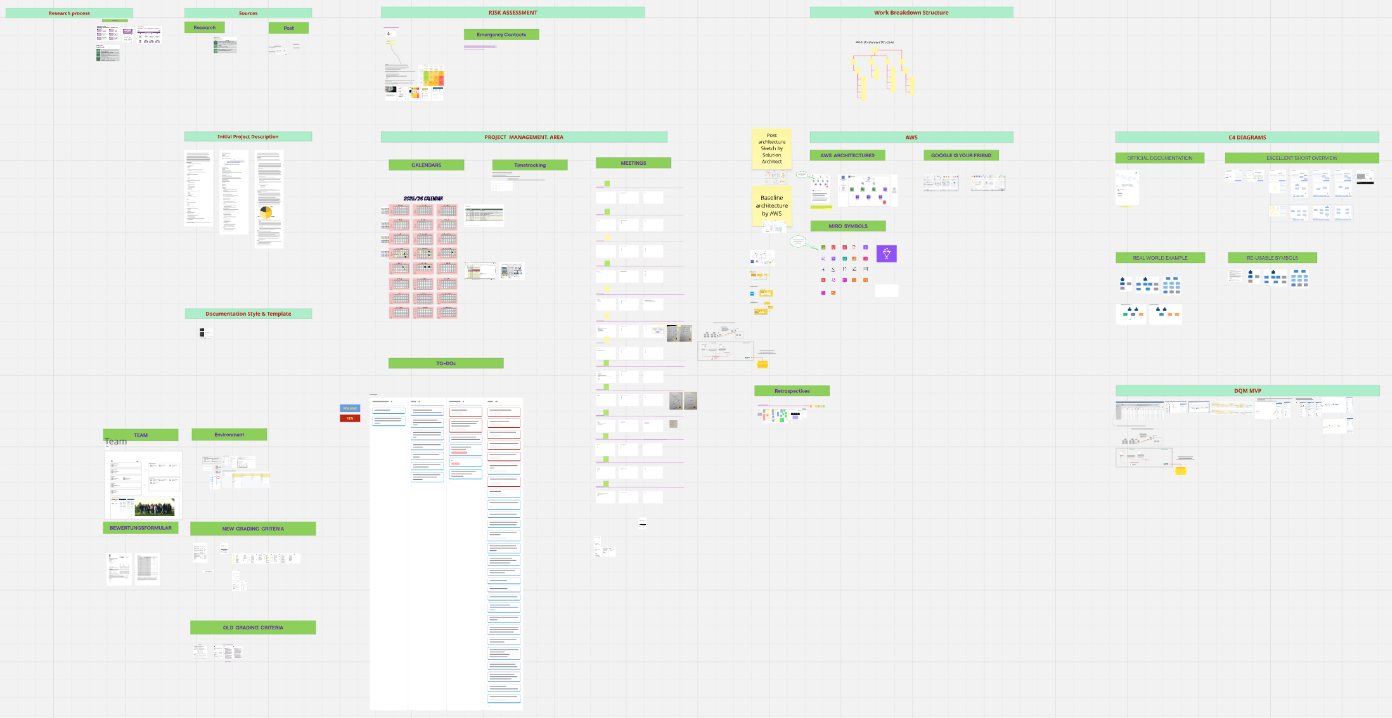
\includegraphics[width=0.8\textwidth]{./content/img/MiroBoard__Old_10-11-2025.png}
    \caption{Miro board documentation, view of 10.11.2025}
    \label{fig:miro_board_tenth_november}
\end{figure}

\begin{figure}[H]
    \centering
    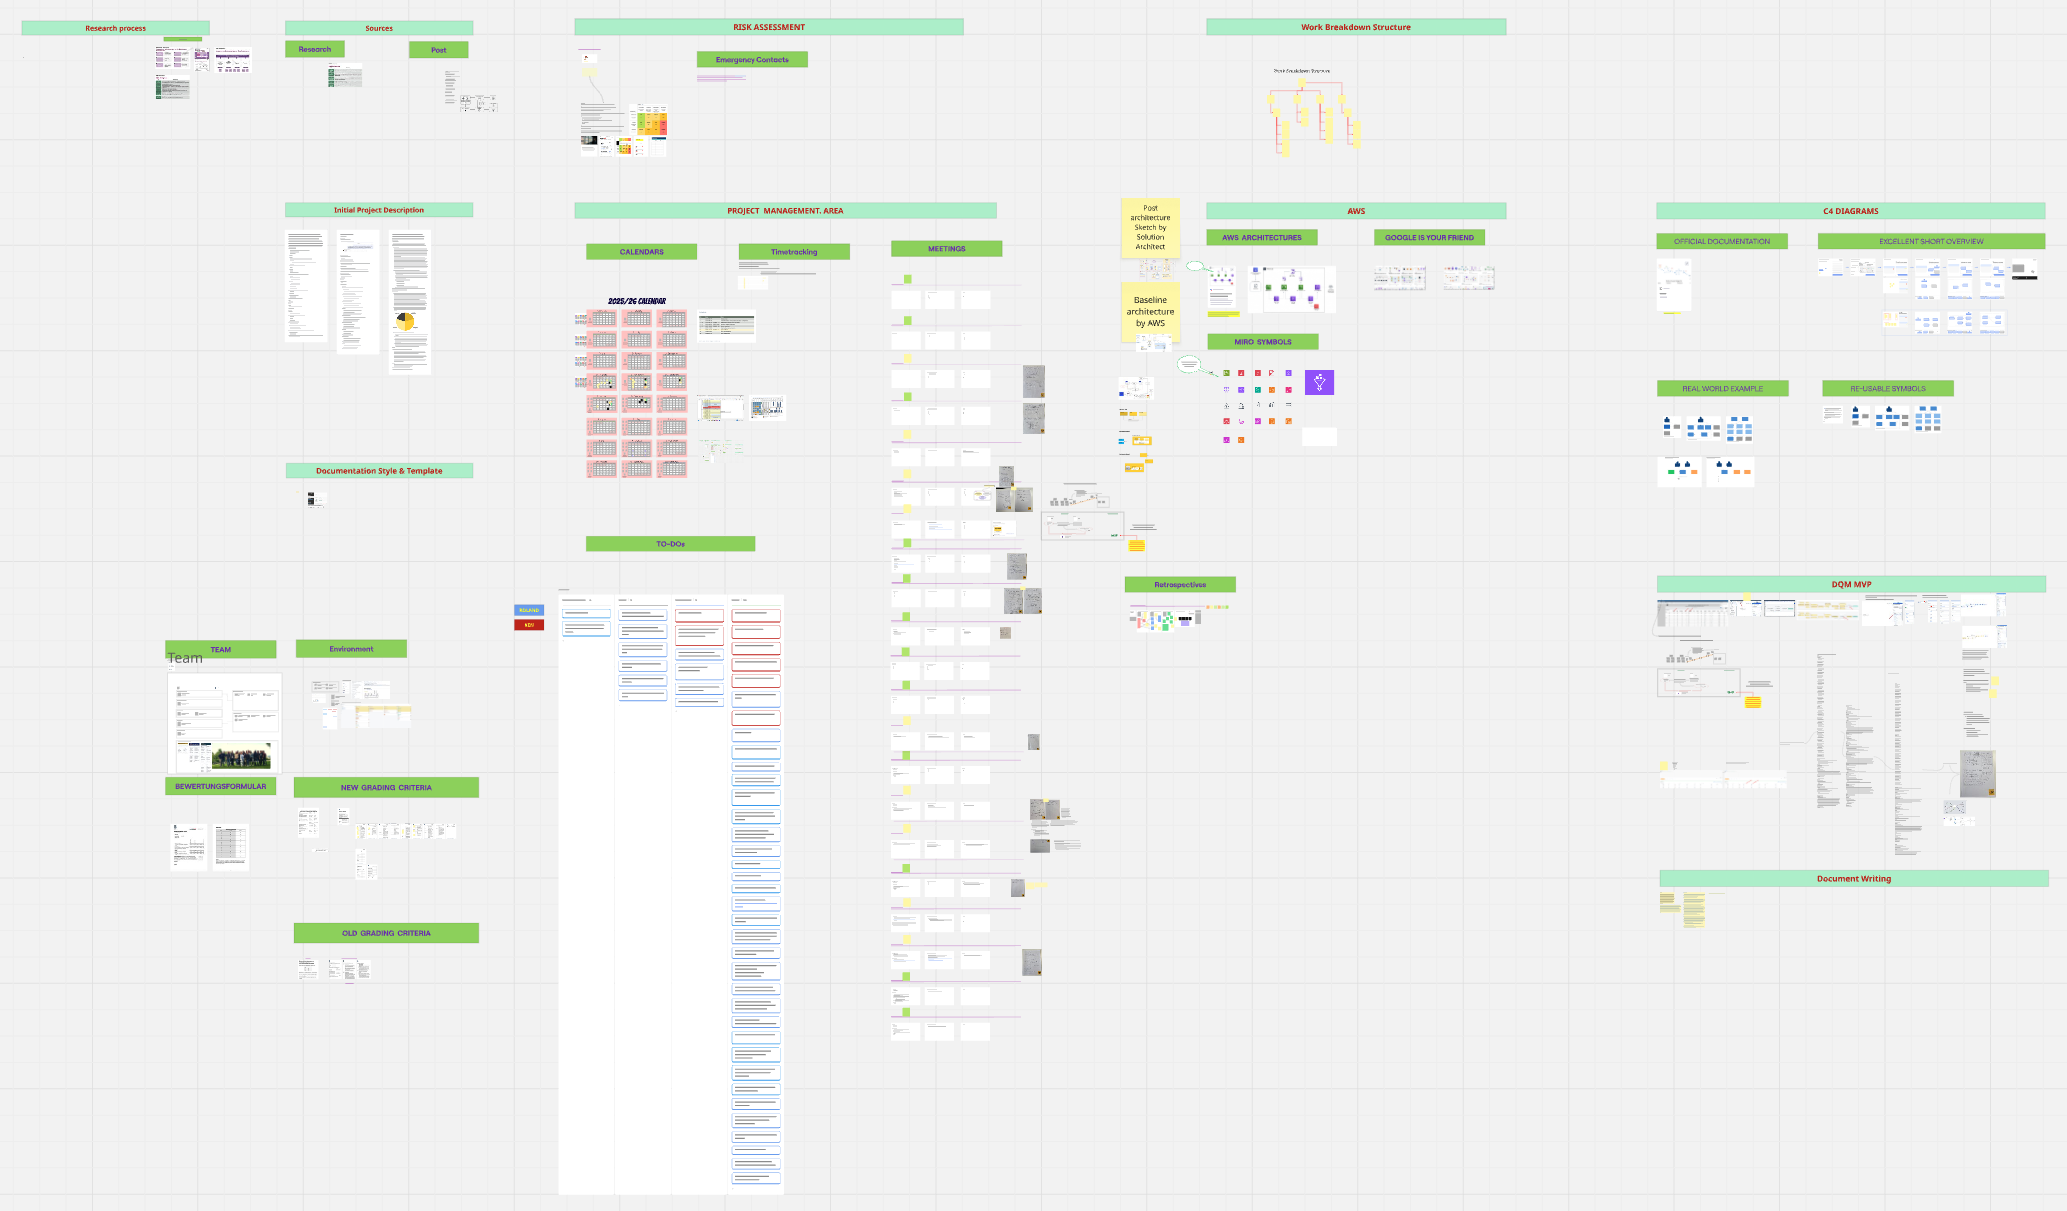
\includegraphics[width=0.8\textwidth]{./content/img/MiroBoard_25-11-2025_15-36-28.png}
    \caption{Miro board documentation, view of 25.11.2025}
    \label{fig:miro_board_twentyfifth_november}
\end{figure}

\begin{figure}[H]
    \centering
    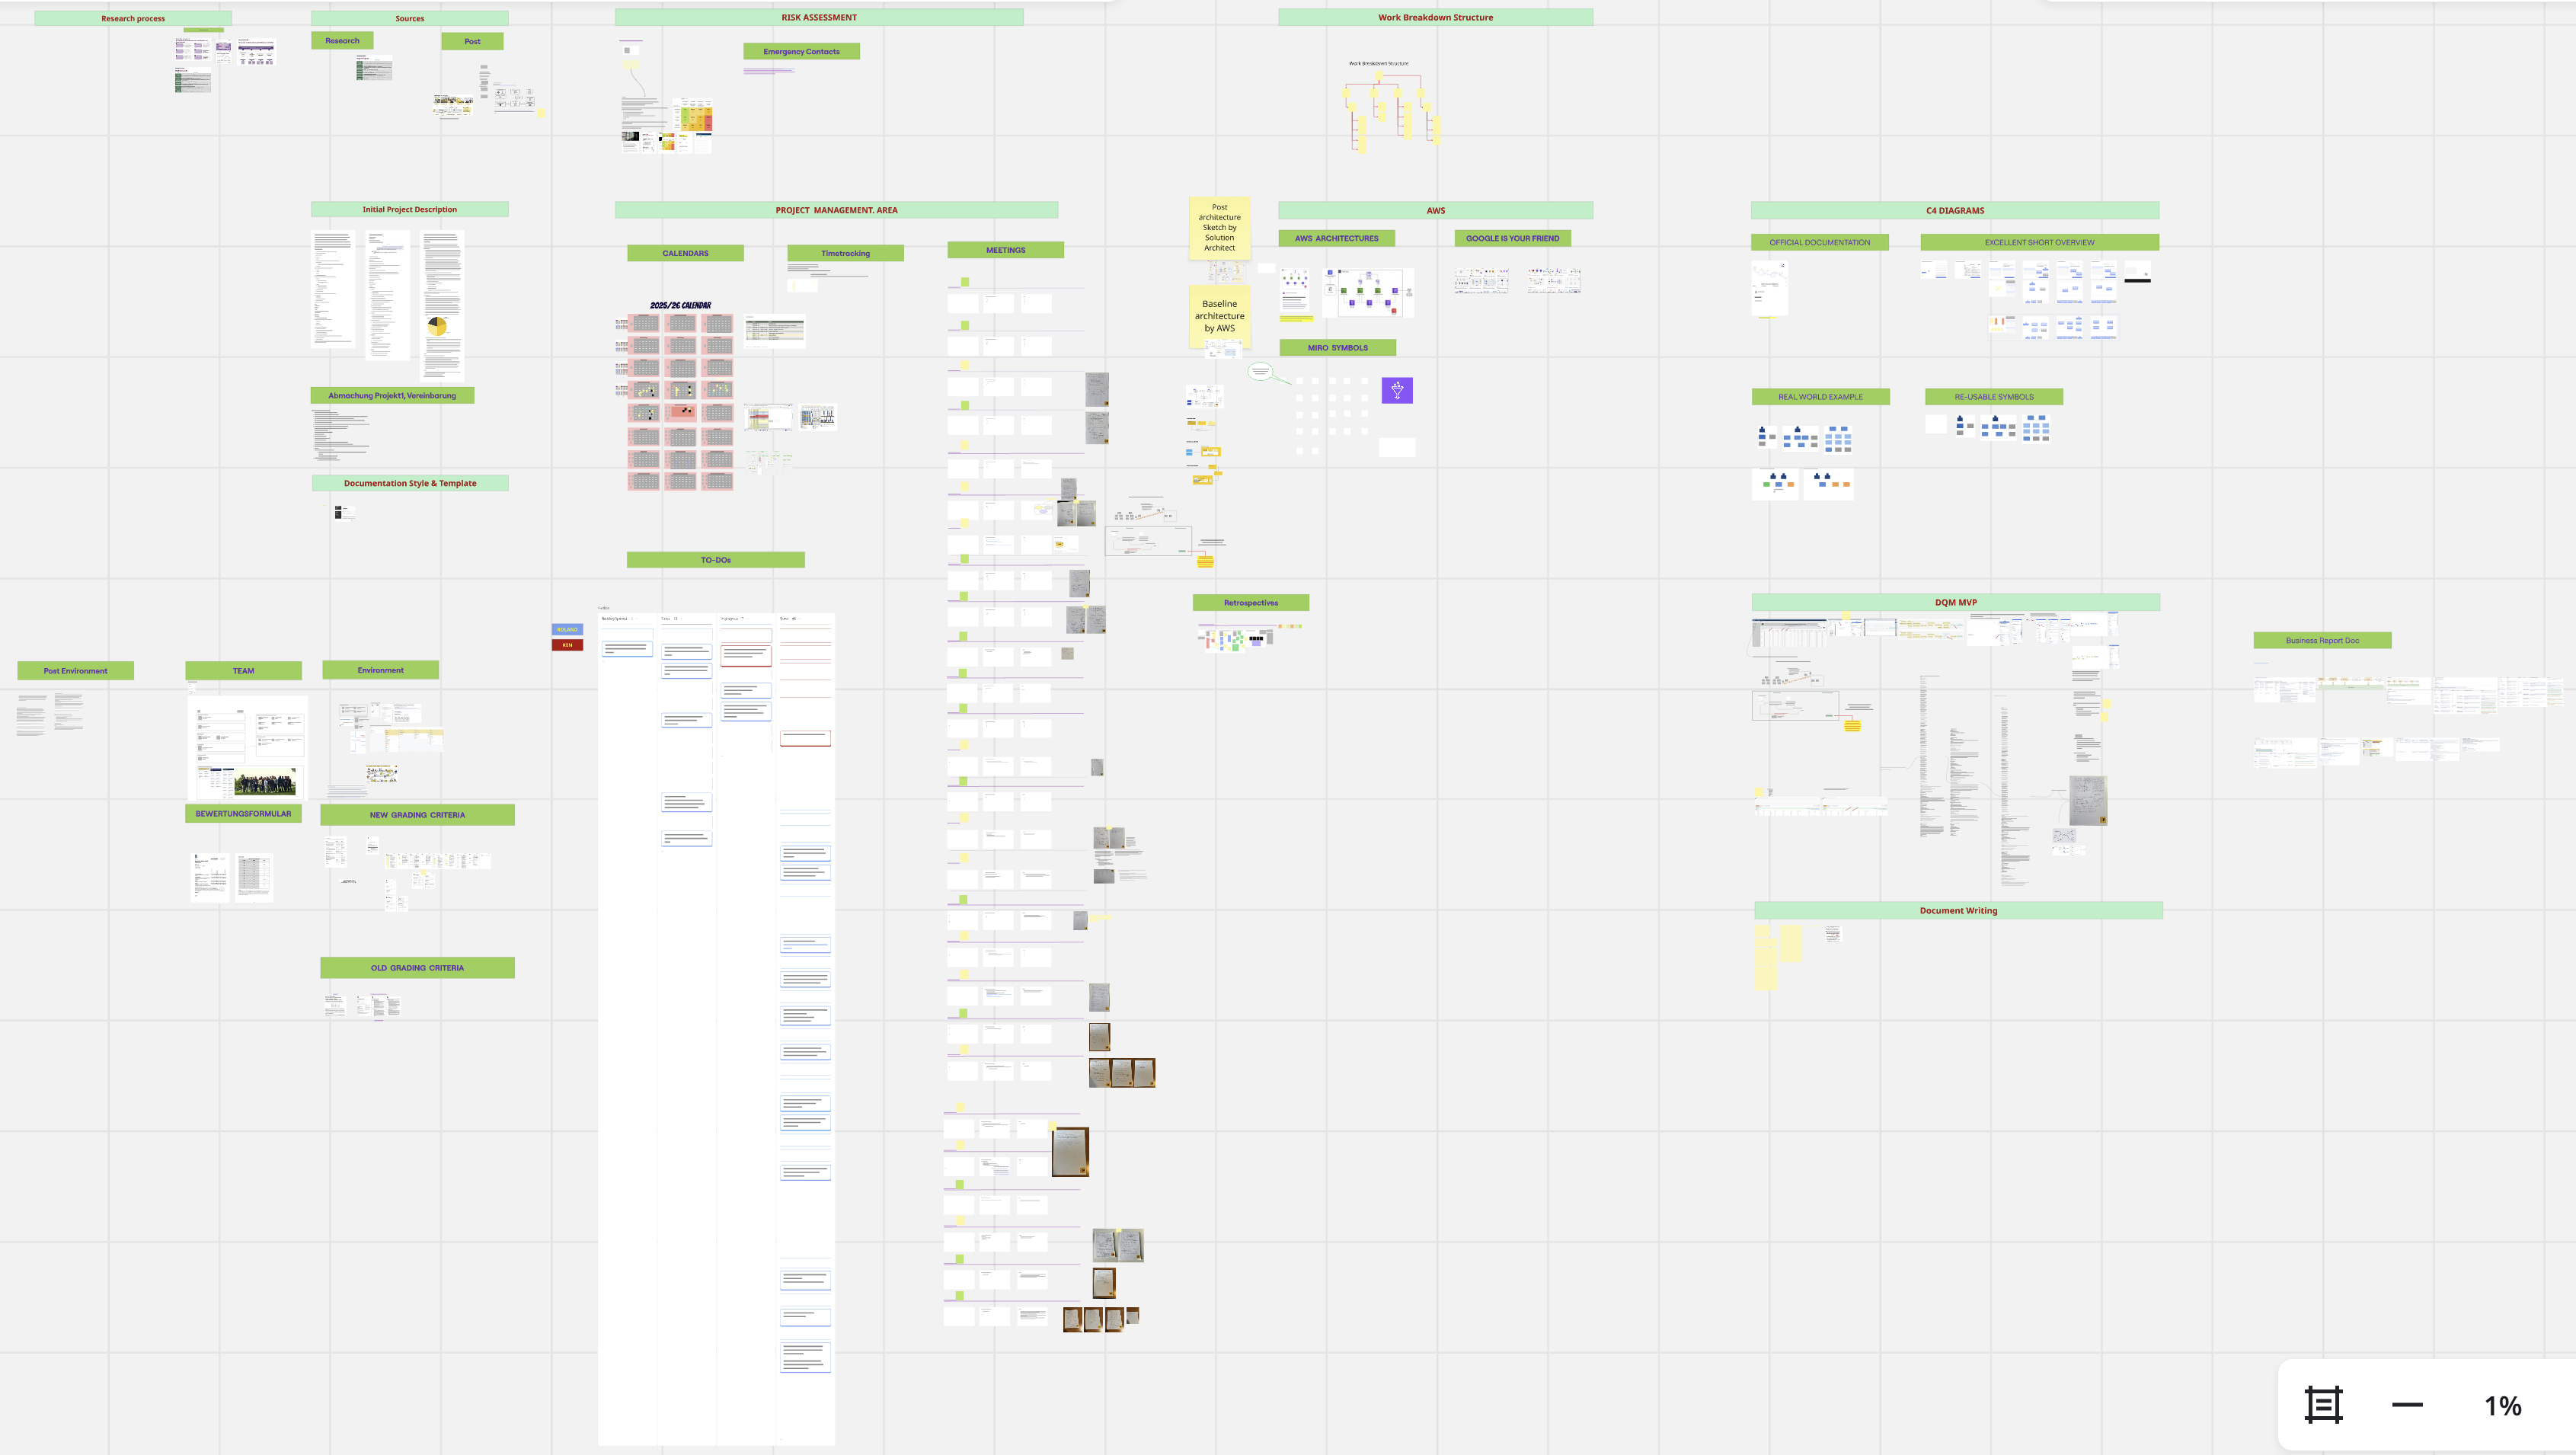
\includegraphics[width=0.8\textwidth]{./content/img/MiroBoard_23-12-2025.png}
    \caption{Miro board documentation, view of 23.12.2025}
    \label{fig:miro_board_twentythird_december}
\end{figure}

\begin{figure}[H]
    \centering
    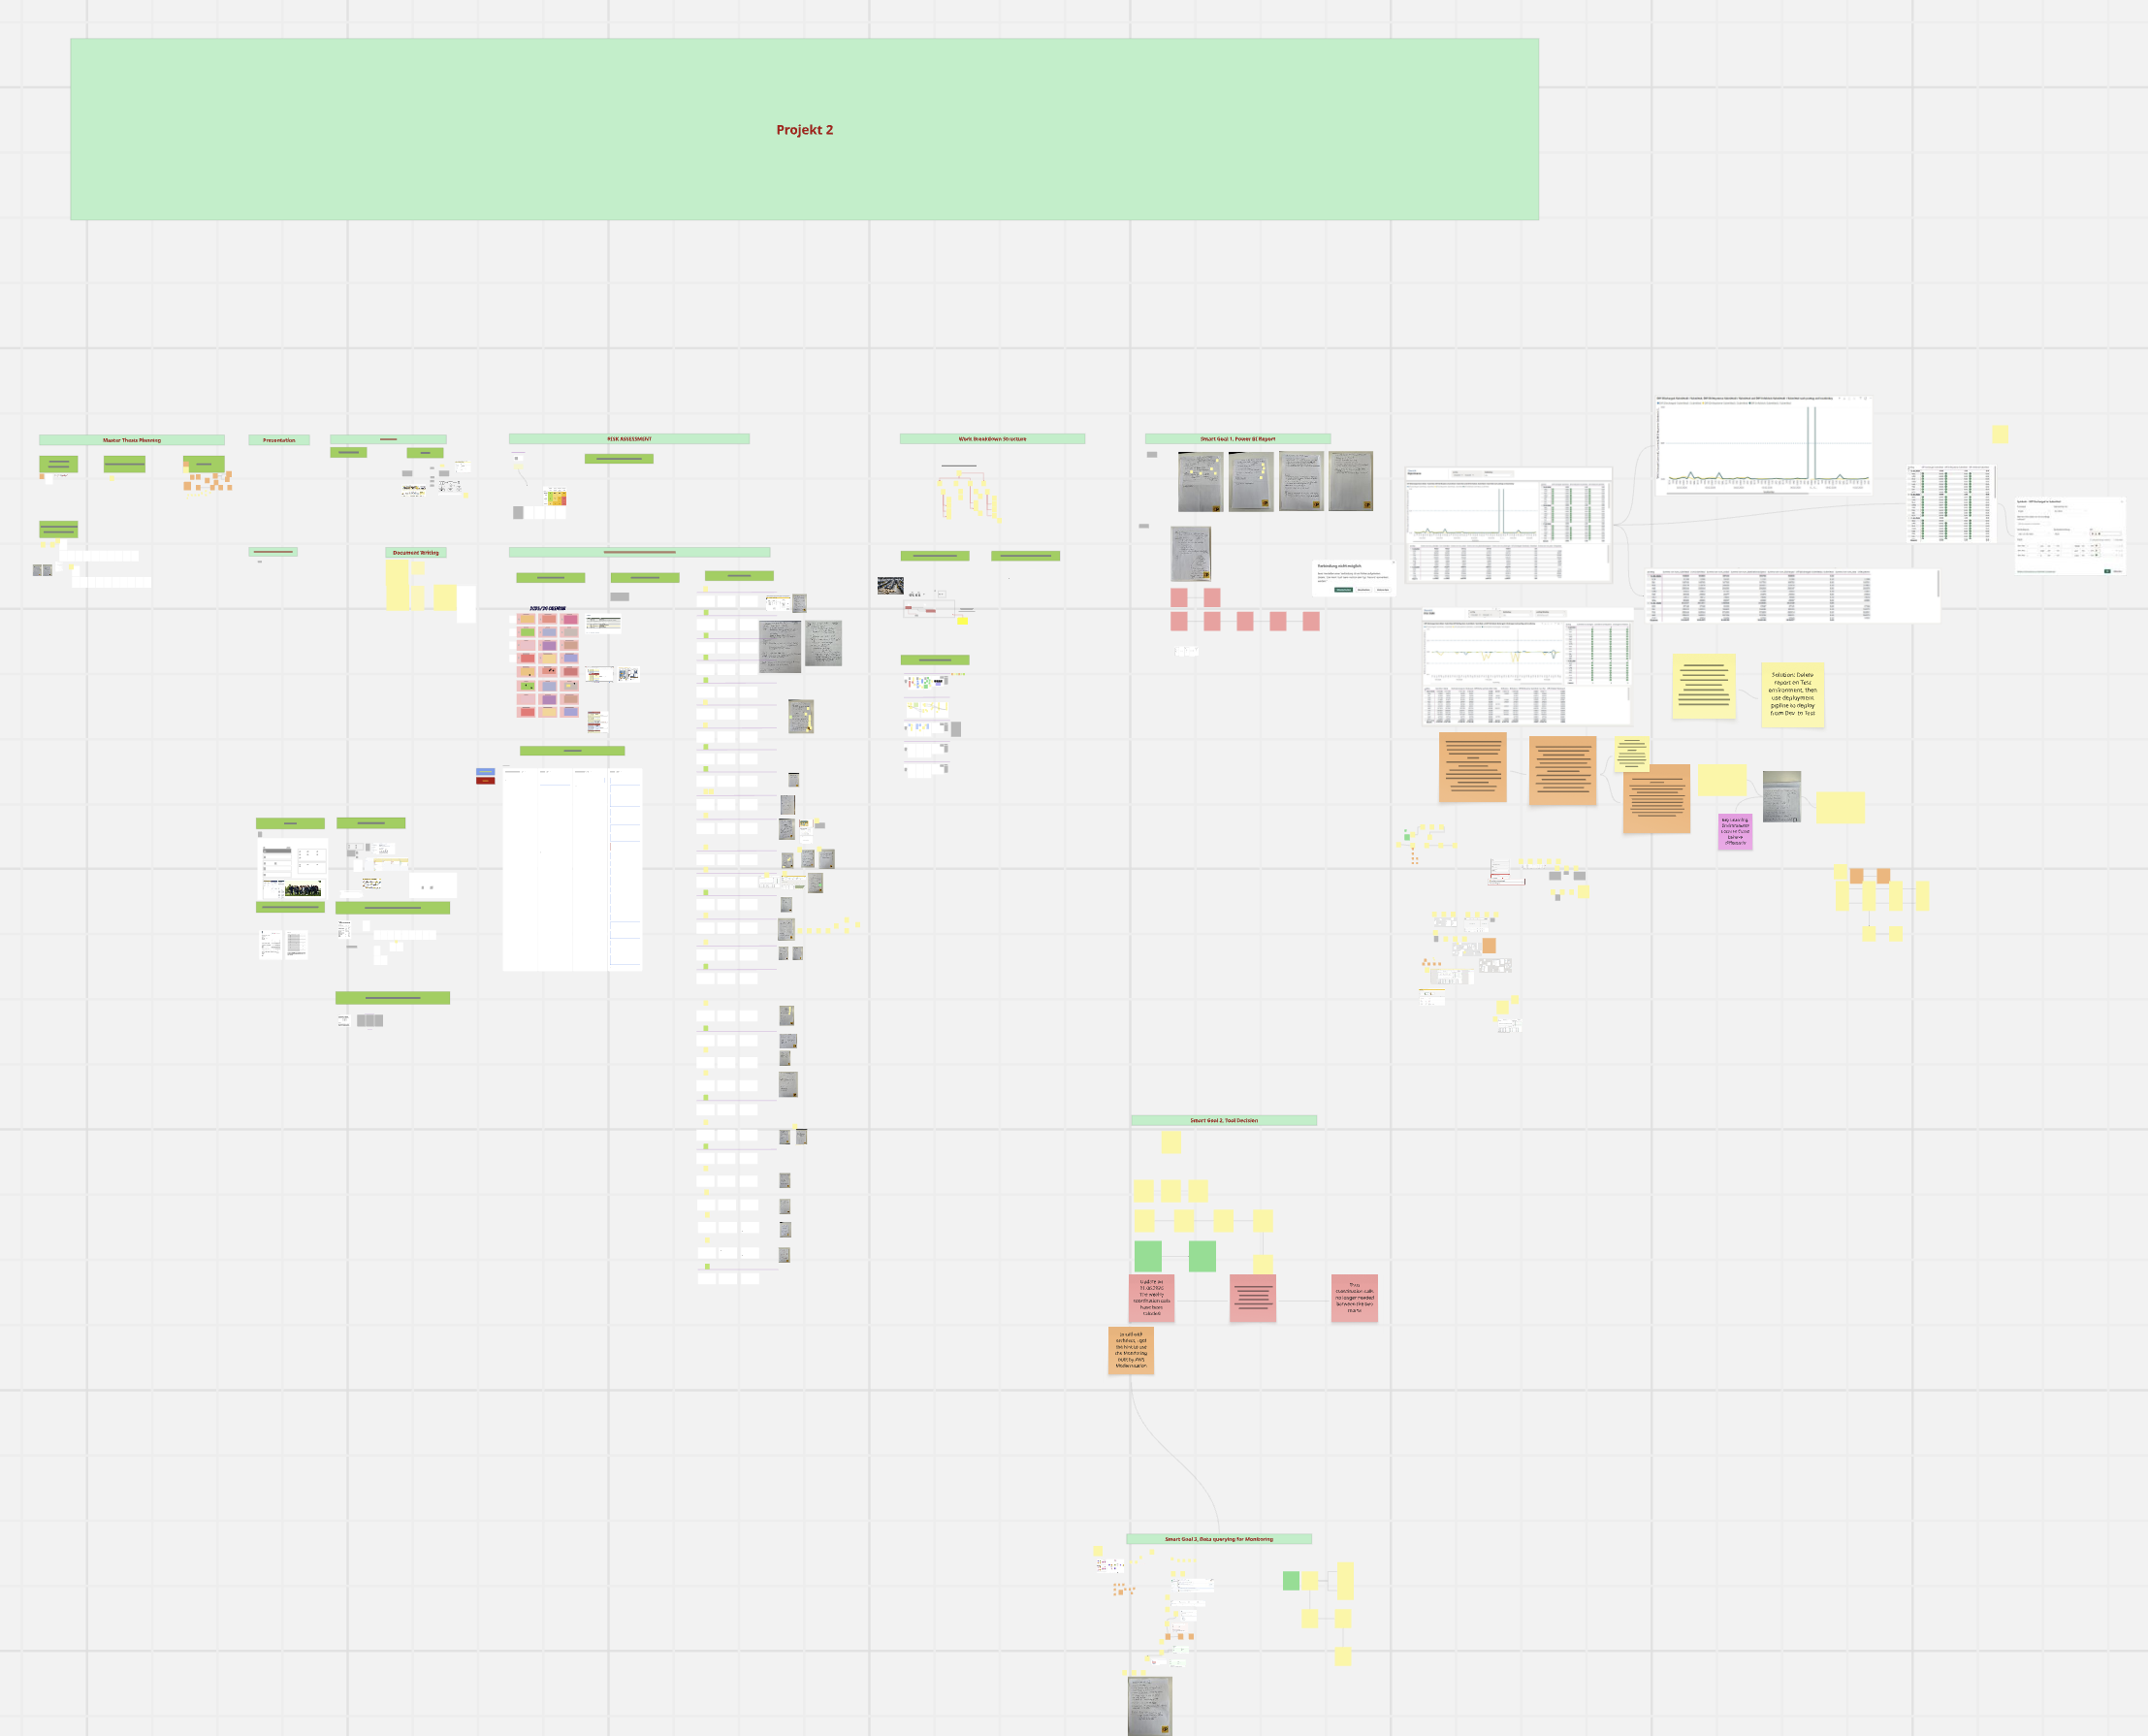
\includegraphics[width=\textwidth]{./content/img/MiroBoard_24_07_2026png.png}
    \caption{Complete Miro board documenting the evolution of the project. The board contains the complete collection of notes, diagrams, screenshots, milestones, implementation artefacts and planning information accumulated during the project. Screenshot taken on 24 July 2026.}
    \label{fig:annex_miro_complete}
\end{figure}


\section{Miro Details of SMART Goals}

The following screenshots provide a high-level overview of the work carried out for the individual SMART Goals. These screenshots are intended only as a reference and are not meant to be readable in detail, but rather to provide a brief overview of the methods used.



\begin{figure}[H]
    \centering
    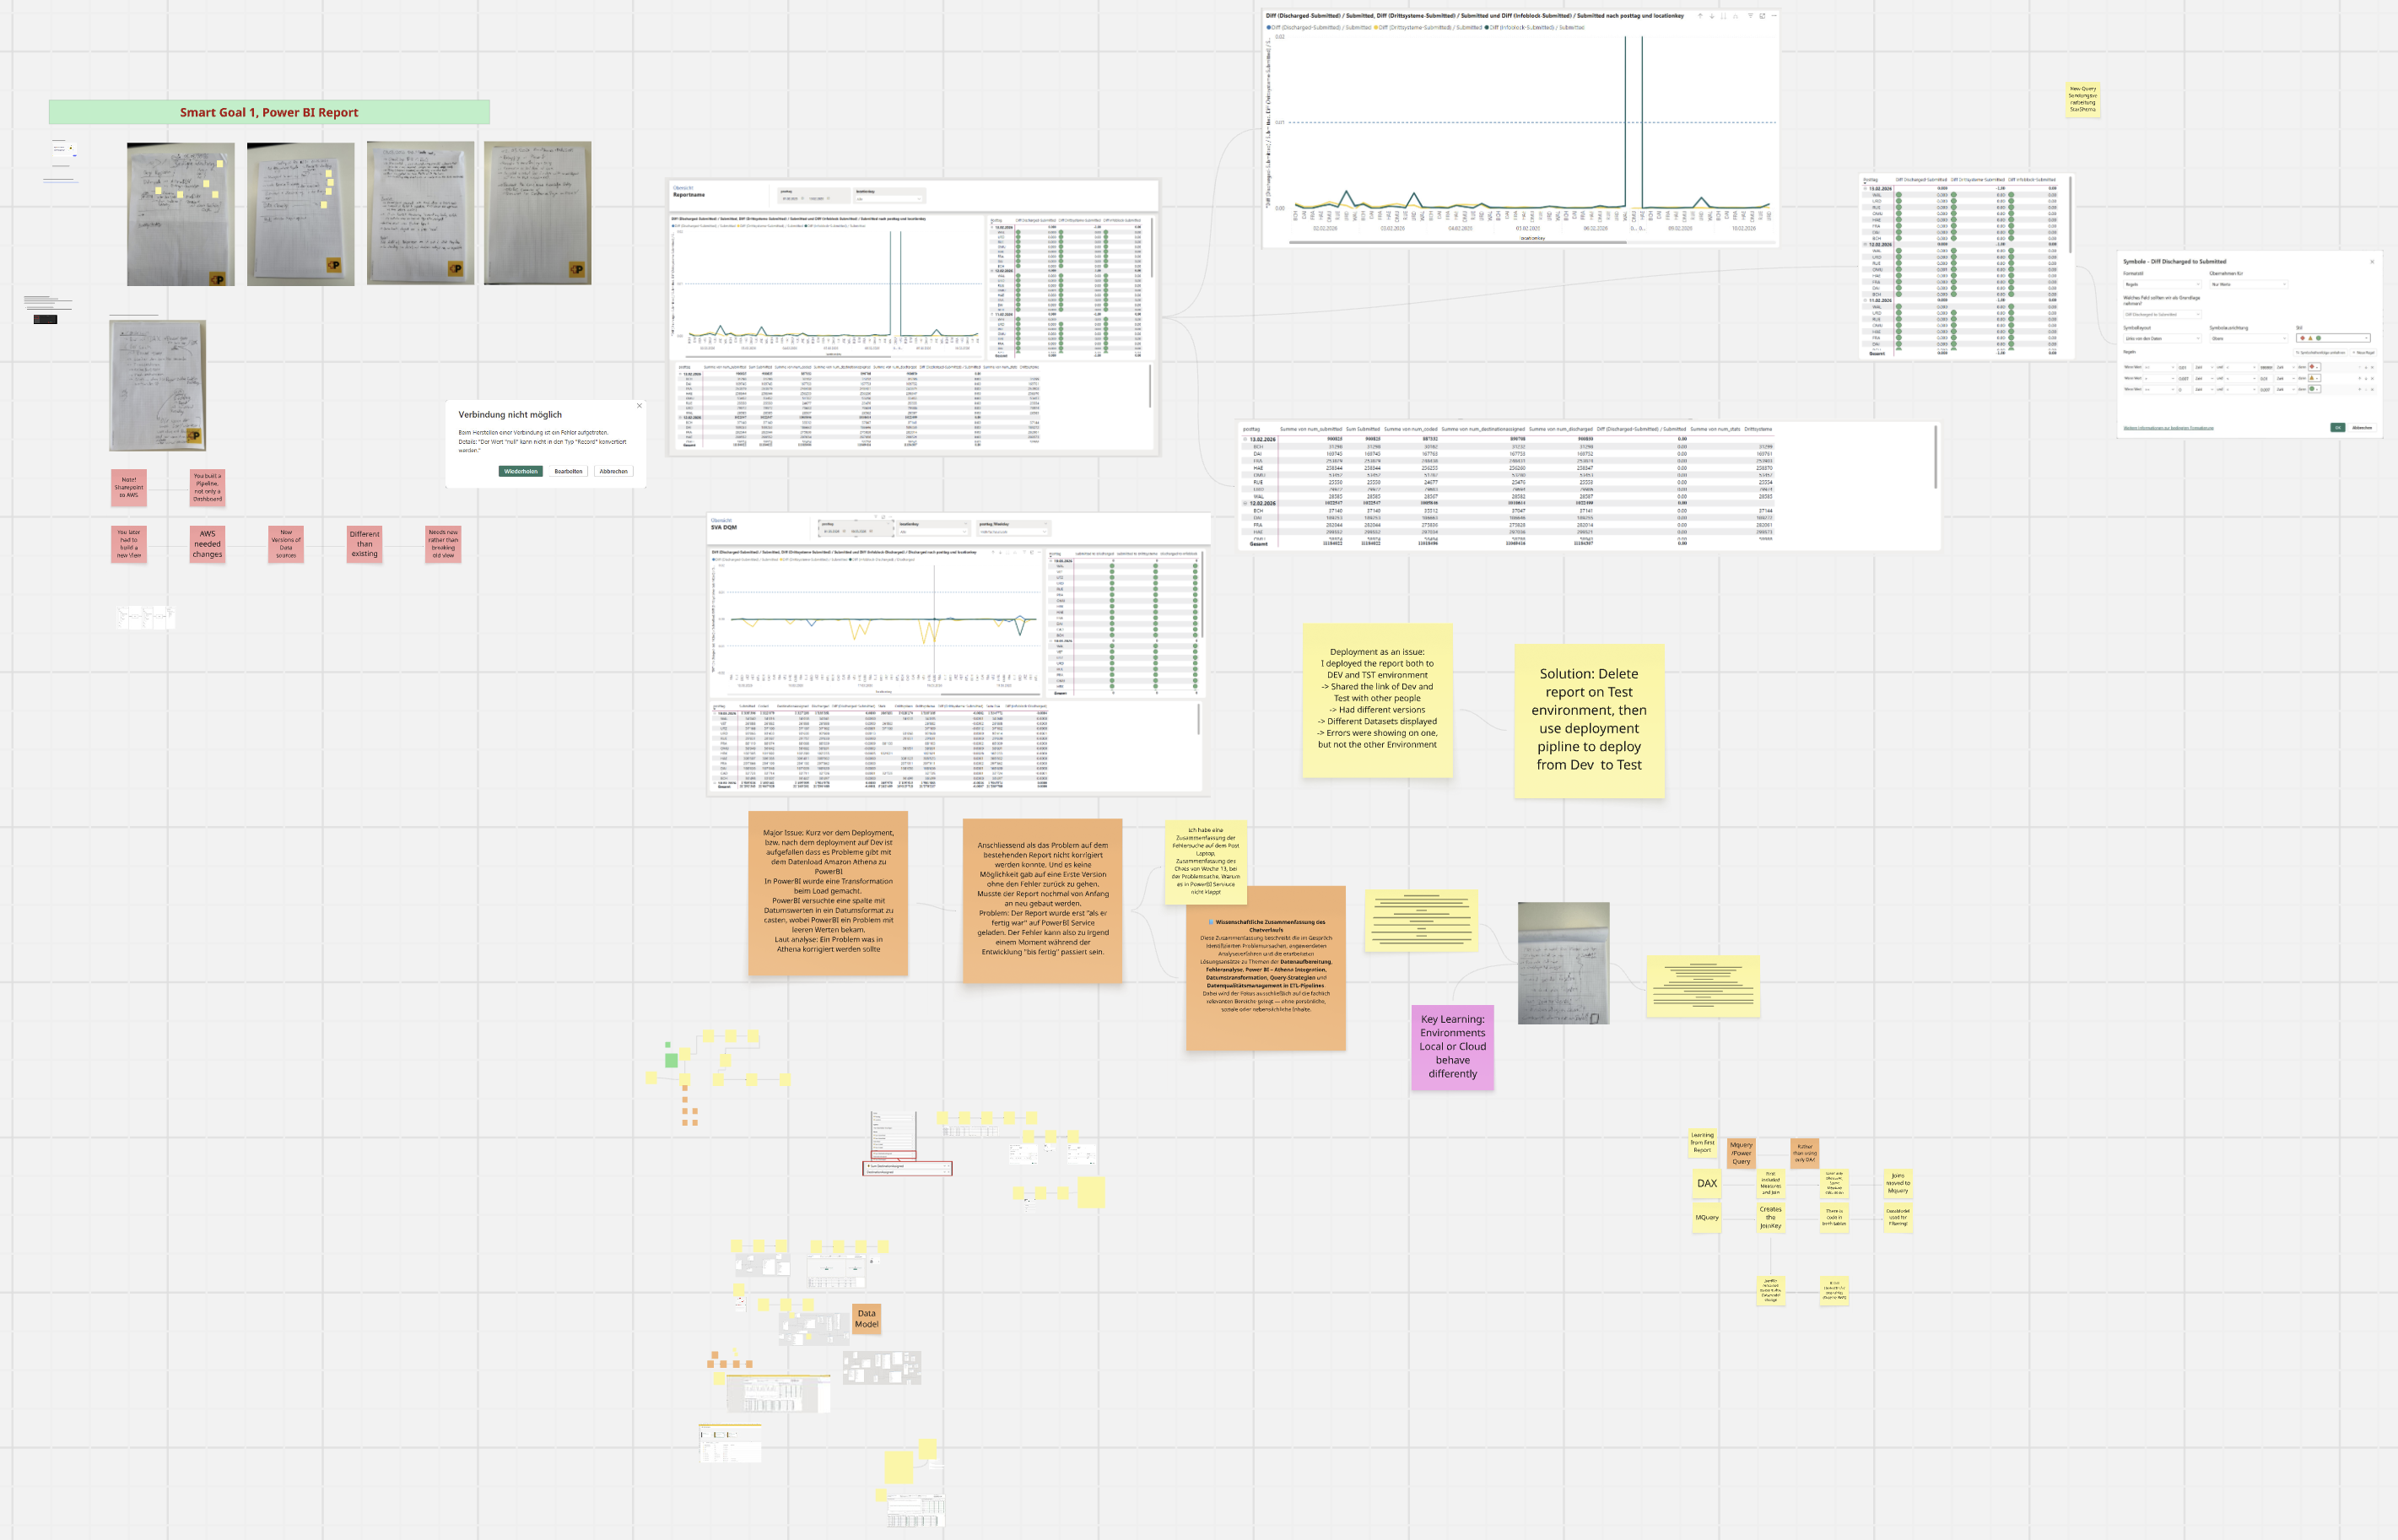
\includegraphics[width=\textwidth]{./content/img/MiroBoard_SmartGoal1.png}
    \caption{Extract of the Miro board related to Smart Goal 1. The board illustrates the planning and documentation of the reporting solution, including design concepts, implementation notes and supporting artefacts collected throughout the project.}
    \label{fig:annex_miro_smartgoal1}
\end{figure}

\begin{figure}[H]
    \centering
    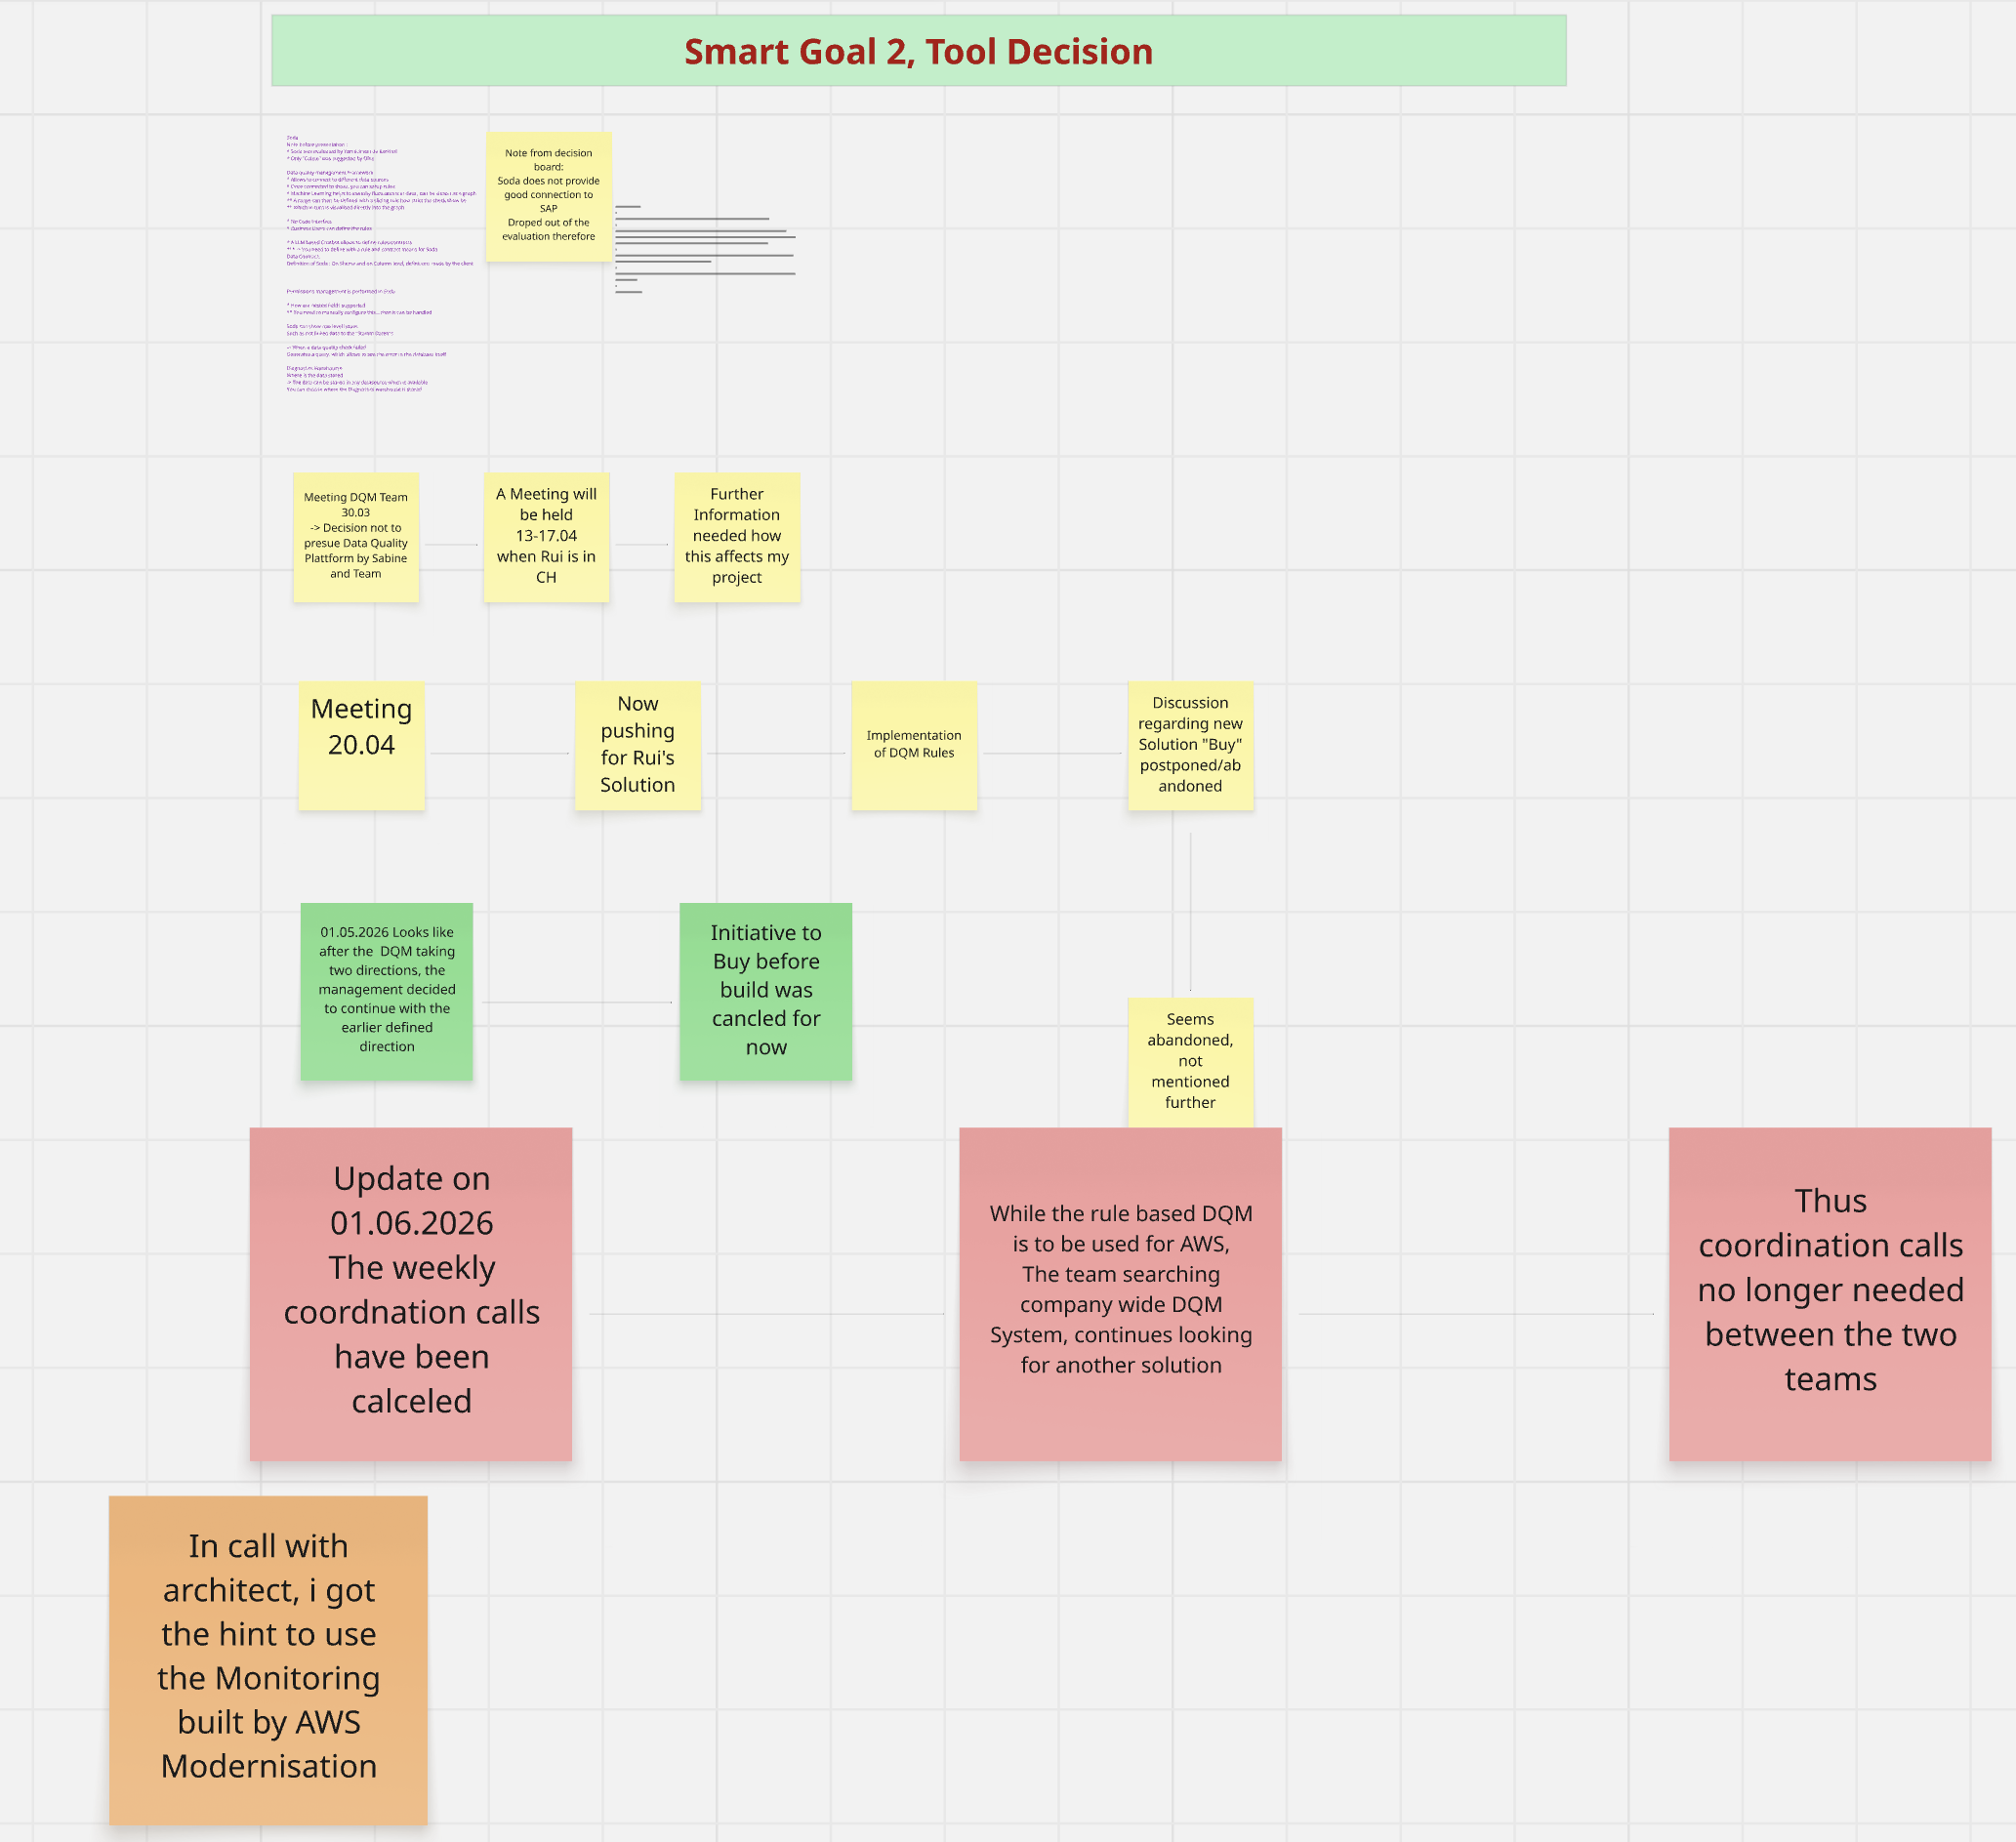
\includegraphics[width=\textwidth]{./content/img/MiroBoard_SmartGoal2.png}
    \caption{Extract of the Miro board related to Smart Goal 2. The material summarises the evaluation activities, comparisons, vendor discussions and supporting documentation used during the assessment of data quality management solutions.}
    \label{fig:annex_miro_smartgoal2}
\end{figure}

\begin{figure}[H]
    \centering
    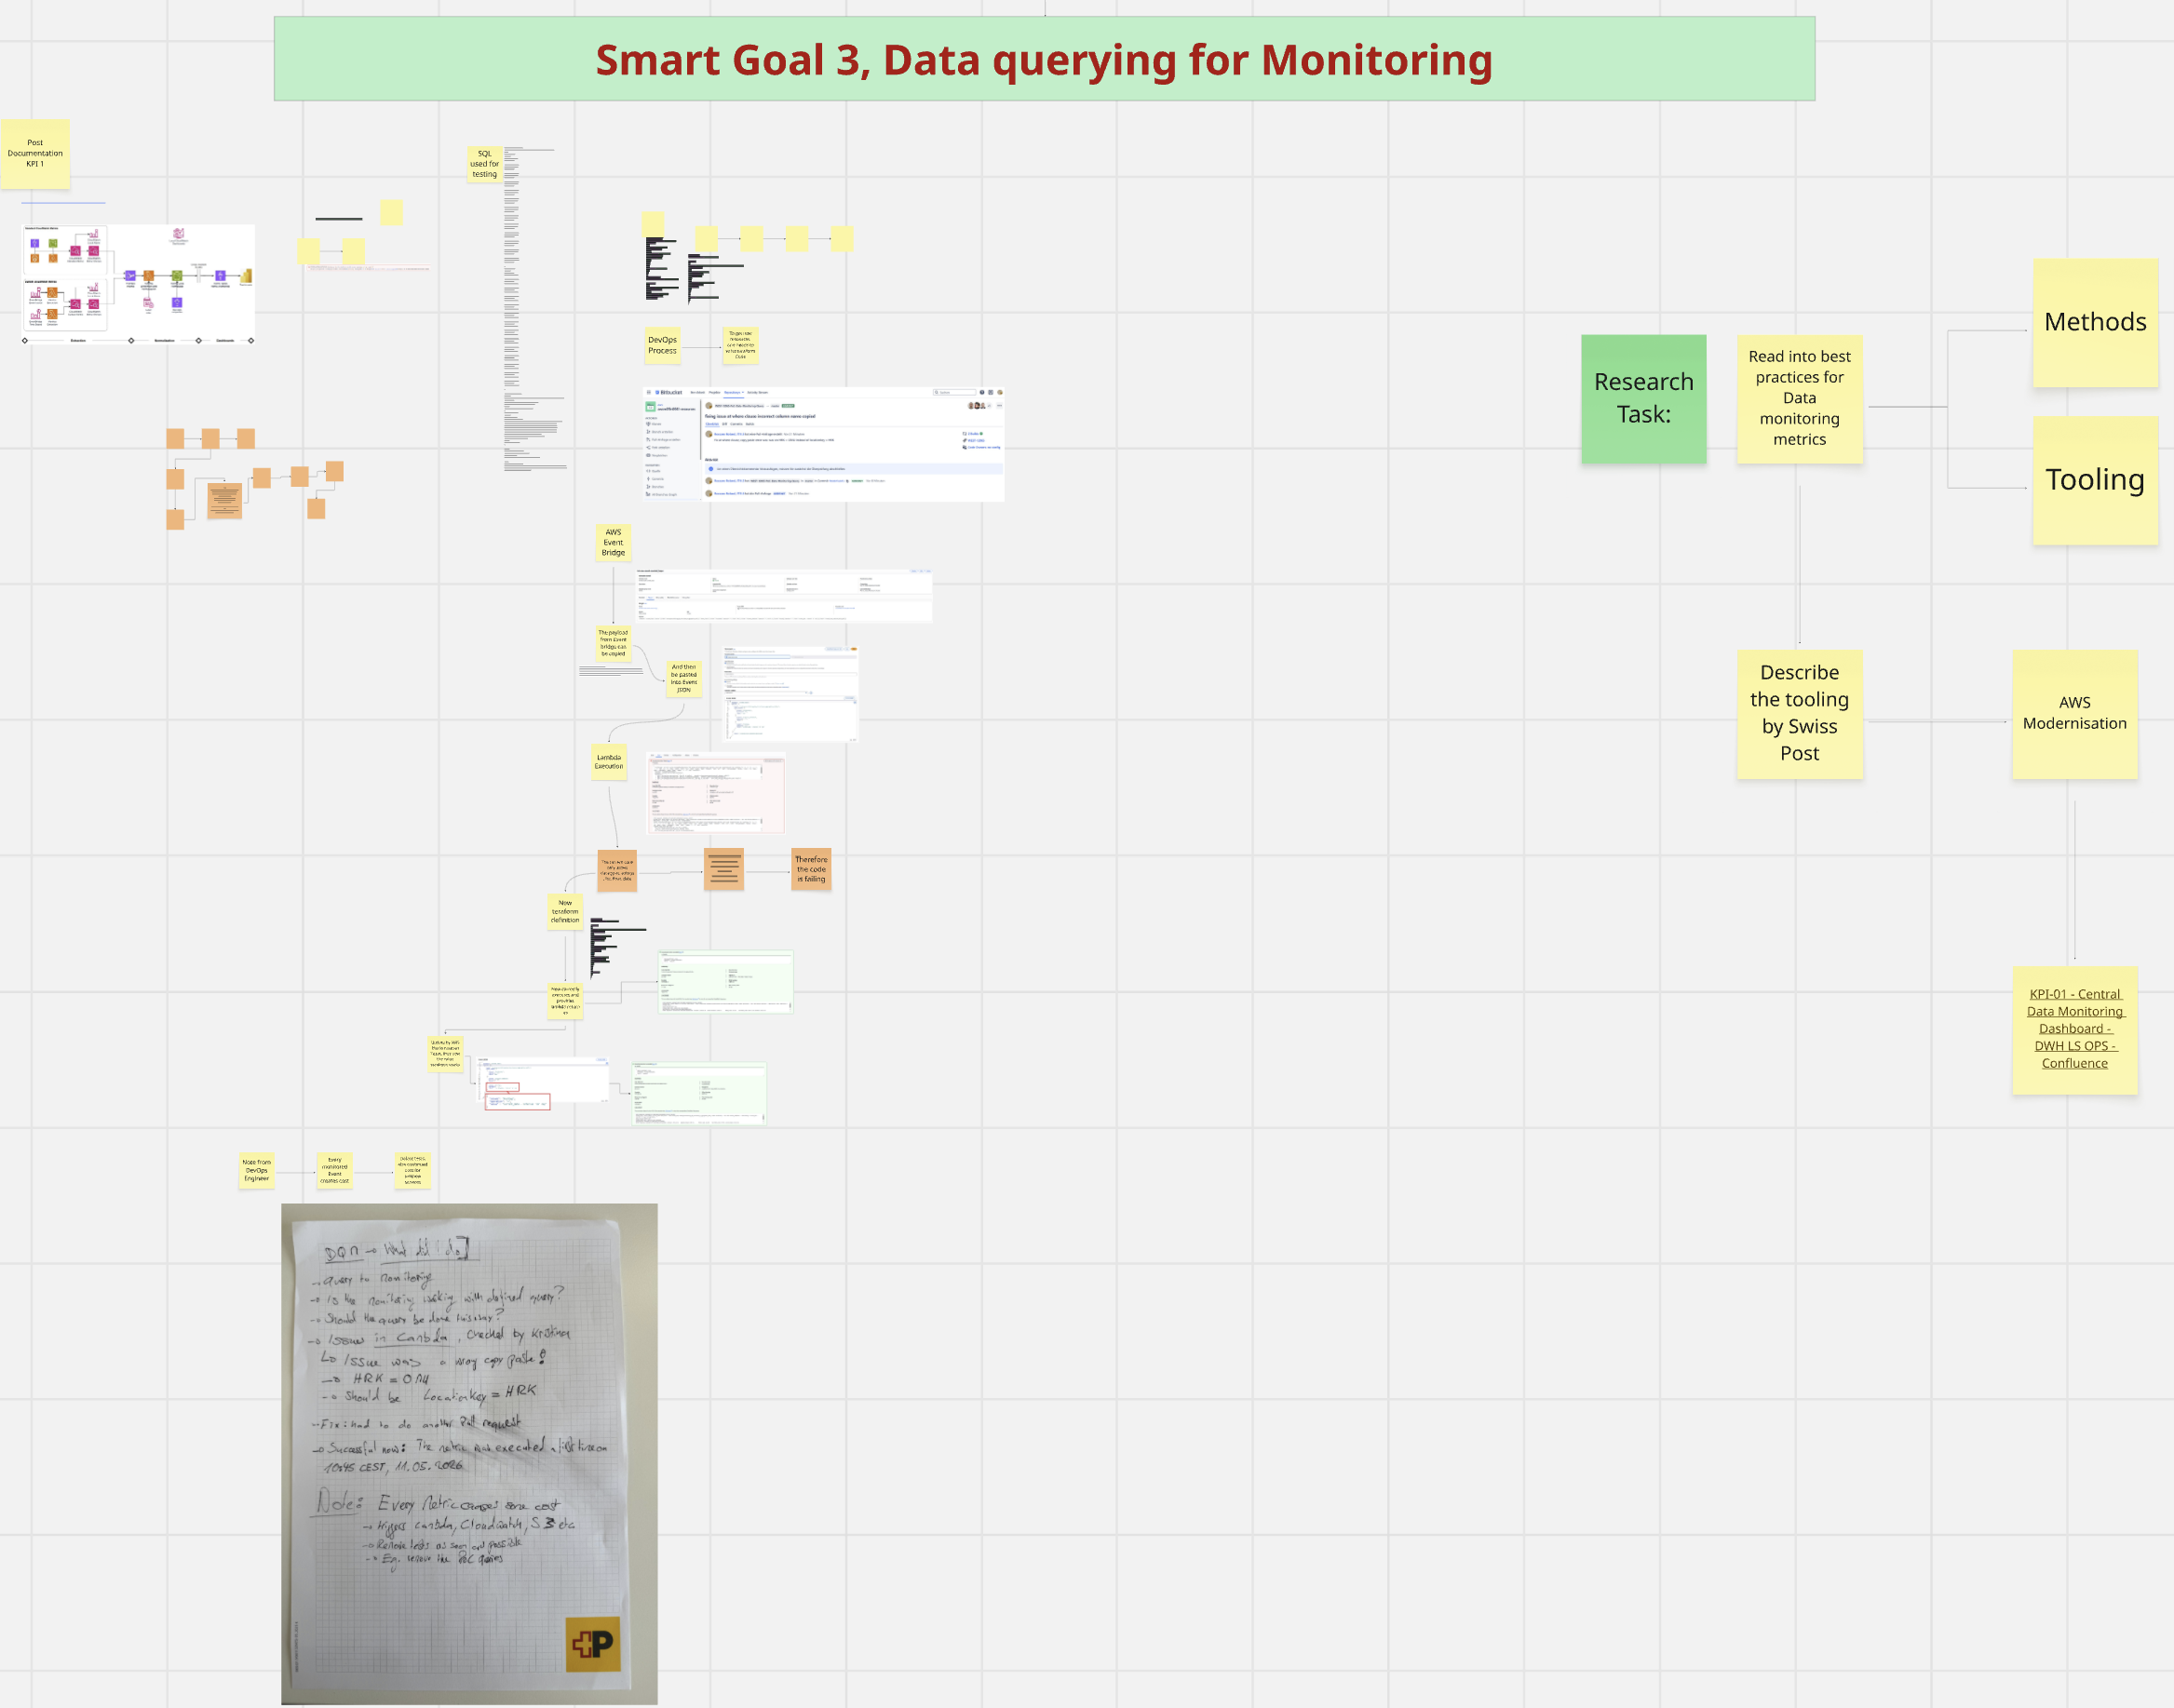
\includegraphics[width=\textwidth]{./content/img/MiroBoard_SmartGoal3.png}
    \caption{Extract of the Miro board related to Smart Goal 3. The board documents the collection of implementation notes, design ideas, intermediate results and decisions supporting the validation of the selected proof-of-concept.}
    \label{fig:annex_miro_smartgoal3}
\end{figure}
\begin{landscape}
\chapter{Risk Monitoring}
\label{RiskMonitoring}
The risk Monitoring files are linked in the following tables.

\subsection*{July 2026 }
A final monitoring performed on 24.07.2026, concluded the writing phase on project 2.



\begin{longtable}{|c|p{4cm}|c|p{3cm}|p{3cm}|p{3cm}|c|}
\hline
\textbf{Number} & \textbf{Risk} & \textbf{Occured} & \textbf{Detail} & \textbf{Why} & \textbf{Measures taken} & \textbf{Measure date} \\ \hline
\endfirsthead

\hline
\textbf{Number} & \textbf{Risk} & \textbf{Occured} & \textbf{Detail} & \textbf{Why} & \textbf{Measures taken} & \textbf{Measure date} \\ \hline
\endhead

1  & Unclear question & No &  &  & Measures taken &  \\ \hline
2  & Unclear goals & No &  & Team Members, PO in team &  &  \\ \hline
3  & Insufficient expertise & Yes & Latex usage to change document structure & Some parts of the used BFH template had to be changed due to amendments with tables and additional content & Used ChatGPT for review and changes & 24.07.2026 \\ \hline
4  & Underestimated time/effort & Yes & Efforts for writing were not committable before holiday & Took too much time in relation to needed cool down times & Moved writing partially to holiday & 24.07.2026 \\ \hline
5  & Other study projects & Yes & No time invested & Focus on this project &  & 24.07.2026 \\ \hline
6  & Work projects & No & In December much more work on the project was possible, no incidents & Full focus on new topics &  &  \\ \hline
7  & Procrastination & No &  & Now time to finish & Working hard during beach holiday & 24.07.2026 \\ \hline
8  & Unavailability of main project staff (e.g., illness) & No &  &  &  &  \\ \hline
9  & Unavailability of advisor (e.g., illness, accident) & No &  &  &  &  \\ \hline
10 & Software Version / Library / Dependency & No &  &  &  &  \\ \hline
11 & Hardware is damaged & No &  &  &  &  \\ \hline
12 & Data related & No &  &  &  &  \\ \hline
13 & Not reproducible work & No &  &  &  &  \\ \hline
14 & Plagiarism or wrong citation & No &  &  &  &  \\ \hline
15 & Copyright & No &  &  &  &  \\ \hline
16 & Bad communication with stakeholder or advisor & No &  &  &  &  \\ \hline
17 & Insufficient exchange with external partners & No &  &  &  &  \\ \hline
18 & Unforeseen familiar crisis & No &  &  &  &  \\ \hline
19 & General force majeure & No &  &  &  &  \\ \hline
20 & Unknown process & Yes & Finally after a lot of back and forth the invoice was handled through sending it via post mail & BFH could not sign the new Terms of Swiss Post & Next invoice to be sent by mail directly & 01.07.2026 \\ \hline

\end{longtable}
\end{landscape}

\clearpage
\chapter{Time Tracking}
\label{AnnexTimeTracking}
Todo
Compare planned chapter / Milestone efforts

This annex section contains the time tracking performed during the course of the project. The content is provided in a raw form without further refinement. This section serves the purpose of transparency. Totals at 11.01.2026 when handing in the project document are: 155.35h at work and 201.28h Off work 201.28h. Total of 356.64h

\section{Efforts at work}
This listing documents efforts during work hours, describing the dates and times when work on the project was carried out, including a short description. Efforts are tracked in the time-tracking and MIAR systems, in which worked hours are allocated to projects. These records reflect the efforts undertaken as part of the professional engagement with Swiss Post.



\section{Efforts outside work}
This section provides the same type of listing as for work efforts, but for efforts carried out outside of working hours. These represent additional efforts performed beyond the engagement during office hours.



  

\end{document}
